\documentclass[SE,lsstdraft,authoryear,toc]{lsstdoc}
% GENERATED FILE -- edit this in the Makefile
\newcommand{\lsstDocType}{SITCOMTN}
\newcommand{\lsstDocNum}{148}
\newcommand{\vcsRevision}{80cc9c9-dirty}
\newcommand{\vcsDate}{2025-01-16}

\usepackage{array}
\usepackage{subcaption}
\usepackage{longtable,booktabs,array}
\usepackage{pgfgantt}
\usepackage{pdflscape}
\usepackage{makecell}  %for multi-line cells in tables

% local declarations
\def\jinst{Journal of Instrumentation}            % JINST
\usepackage{anyfontsize} 

% compile error mitigations
\setlength{\headheight}{61.9707pt}
\setmonofont{Inconsolata}

%\hypersetup{
%  pdftitle={LSSkT Camera Electro-Optical Test Results},
%  hidelinksk,
%  pdfcreator={LaTeX via pandoc}}

\providecommand{\tightlist}{%
  \setlength{\itemsep}{0pt}\setlength{\parskip}{0pt}}

%If you want glossaries
%\input{aglossary.tex}
%\makeglossaries

\title{LSST Camera Electro-Optical Test (Run~7) Results}

% Optional subtitle
% \setDocSubtitle{A subtitle}

\author{% ordered in alphabetical (last name)
The LSST Camera group:
Pierre Antilogus,
Pierre Astier,
John Banovetz,
James Chiang,
Seth Digel,
Kevin Fanning,
Yassine Faris,
Thibault Guillemin,
Tony Johnson,
Claire Juramy,
Craig Lage,
Shuang Liang,
Sean MacBride,
Stuart Marshall,
Homer Neal,
Daniel Polin,
Andrew Rasmussen,
Aaron Roodman,
Eli Rykoff,
Brian Stalder,
Gregg Thayer,
Tony Tyson,
HyeYun Park,
Yousuke Utsumi,
Zhuoqi Zhang
}

\setDocRef{SITCOMTN-148}
\setDocUpstreamLocation{\url{https://github.com/lsst-sitcom/sitcomtn-148}}

\date{\vcsDate}

% Optional: name of the document's curator
% \setDocCurator{The Curator of this Document}

\setDocAbstract{%
This note collects results from the LSST Camera electro-optical testing
prior to installation on the TMA. We describe the focal plane
characterization, optimization, and the resulting default settings. Results from eo-\phantomsection\label{pipe}{pipe} are shown for standard runs such as B-protocols, Dense and SuperDense PTCs, gain stability, OpSim runs of
Darks, and Darks with variable delays. We also describe features such as
e2v Persistence, ITL phosphorescence in coffee stains, remnant charge
near Serial register following saturated images, vampire pixels, ITL
dips, and other sensor features.
}

% Change history defined here.
% Order: oldest first.
% Fields: VERSION, DATE, DESCRIPTION, OWNER NAME.
% See LPM-51 for version number policy.
\setDocChangeRecord{%
  \addtohist{1}{YYYY-MM-DD}{Unreleased.}{}
}


\begin{document}


% Create the title page.
\maketitle
% Frequently for a technote we do not want a title page  uncomment this to remove the title page and changelog.
% use \mkshorttitle to remove the extra pages
%\mkshorttitle

\textbf{Introduction} \\
The LSST Camera was constructed at the SLAC National Accelerator Laboratory in California, US. Its functionality and performance were evaluated through various integration phases, leading to the identification and mitigation of non-ideal features.
%\textbf{Transportation and Installation} \\
In May 2024, LSST Camera was transported from Menlo Park to Cerro Pachón, Chile, where the Vera C. Rubin Observatory is being constructed. The Camera was installed in the clean room (White Room) on Level 3 of the observatory. After connecting power and cooling lines and verifying the vacuum performance, the Camera underwent the seventh series of electro-optical (EO) testing (Run 7) from September 2024 to December 2024, collecting 56,066 exposures. This report describes the results from Run 7.

\textbf{Key Testing Points} \\
\begin{itemize}
    \item \textit{Testing Setup Differences}: The EO test setup in the White Room differed from previous setups, primarily using the CCOB Wide Beam projector with a new diffuser system.
    \item \textit{Performance Verification Post-Transportation}: The Camera's performance was reverified after transportation to ensure it matched the pre-transportation checks.
    \item \textit{Optimization of Features}: Previous EO testings identified issues such as persistence and bias instability, which were optimized during Run 7.
    \item \textit{Camera Performance Post-Optimization}: The Camera's performance was evaluated after implementing optimizations.
    \item \textit{Investigation of Other Features}: Additional sensor features were investigated.
    \item \textit{Summary of Run 7 Operations and Issues}: Overall operations and issues encountered during Run 7 were summarized.
\end{itemize}

\textbf{Electro-Optical Setup} \\
\begin{itemize}
    \item \textit{Run 7 Optical Modifications}: The EO test setup in the White Room included a cone attached to the L1 cover and a shroud to create a dark environment. A diffuser was installed to reduce weather patterns and uniformly illuminate the focal plane.
    \item \textit{Projector Spots}: A 4K projector was used for EO testing, illuminating all 3206 amplifiers. The projector's background illumination posed challenges, but adjustments were made to improve contrast.
    \item \textit{Dark Current and Light Leaks}: Initial measurements identified light leaks, which were mitigated by covering gaps and using a blackout fabric shroud.
\end{itemize}

\textbf{Reverification} \\
\begin{itemize}
    \item \textit{Background}: EO camera test data was processed to extract key metrics. The primary concern was maintaining performance characteristics between Run 6 and Run 7.
    \item \textit{Stability Flat Metrics}: Charge transfer inefficiency (CTI) measurements showed consistent performance between runs.
    \item \textit{Dark Metrics}: Dark current measurements indicated improved performance, likely due to better shrouding.
    \item \textit{Bright Defects}: Bright defects were evaluated, showing a small increase in Run 7.
    \item \textit{Flat Pair Metrics}: Linearity and PTC turnoff metrics were consistent, with minor differences in e2v sensors due to voltage changes.
\end{itemize}

\textbf{Camera Optimization} \\
\begin{itemize}
    \item \textit{Persistence Optimization}: Persistence issues were addressed by adjusting operating voltages, significantly reducing residual signals.
    \item \textit{Impact on Full-Well}: Reducing the parallel swing voltage decreased the full-well capacity by 22\%.
    \item \textit{Impact on Brighter-Fatter Effect}: The brighter-fatter effect increased slightly but remained within acceptable levels.
    \item \textit{Sequencer Optimization}: Several sequencer configurations were tested to improve performance, including changes to the clear method and toggling the RG bit during parallel transfer.
\end{itemize}

\textbf{Characterization \& Performance Stability} \\
\begin{itemize}
    \item \textit{Final Characterization}: Key metrics from initial and final Run 7 configurations were compared, showing high consistency.
    \item \textit{Stability Flat Metrics}: Serial and parallel CTI measurements remained stable.
    \item \textit{Dark Metrics}: Dark current and bright defect measurements were consistent, with improvements in some rafts.
    \item \textit{Flat Pair Metrics}: Linearity and PTC turnoff metrics showed minor changes, primarily in e2v sensors.
    \item \textit{PTC Gain}: PTC gain measurements were consistent, with a slight increase in e2v sensors.
    \item \textit{Read Noise}: Read noise remained stable across runs.
    \item \textit{PTC Noise}: PTC noise measurements showed no significant deviations.
    \item \textit{Brighter-Fatter Coefficients}: The brighter-fatter effect increased slightly in e2v sensors.
    \item \textit{Row-Means Variance}: Row-means variance showed a slight decrease in e2v sensors.
    \item \textit{Divisadero Tearing}: Divisadero tearing was significantly reduced in e2v sensors.
    \item \textit{Dark Defects}: Dark defect counts remained consistent.
    \item \textit{Persistence}: Persistence was minimized in e2v sensors, with sub-ADU levels across the LSST bandpass.
\end{itemize}

\textbf{Sensor Features} \\
\begin{itemize}
    \item \textit{Tree Rings}: Tree rings are concentric variations in silicon doping concentration observed in flat images. The centers of the tree rings were measured for all 189 LSST Camera science sensors, showing consistent positions around the average center for each direction.
    \item \textit{ITL Dips}: ITL dips were investigated using spot and rectangle projections. No evidence of ITL dips was found in the lab data, but further investigation is needed for on-sky data.
    \item \textit{Vampire Pixels}: Vampire pixels are characterized by a group of pixels with high photo-response surrounded by pixels with low photo-response. These features were identified on ITL sensors and correlated with phosphorescence.
    \item \textit{Phosphorescence}: Phosphorescence was observed in some ITL sensors, showing a transient signal after exposure. The effect was dependent on the HV Bias state and varied with wavelength and signal level.
\end{itemize}

\textbf{Operations and issues} \\
\begin{itemize}
    \item \textit{Camera Control Network Performance}: Network issues were addressed by simplifying the network configuration and upgrading the control system.
    \item \textit{REB PS Power Trip}: Power trips were mitigated by grounding the Utility Trunk door and implementing ESD controls.
    \item \textit{FES Latch Sensor Failure}: A faulty cable was replaced, resolving the issue.
    \item \textit{PCS Degradation}: Performance degradation was managed through various mitigation strategies, with further analysis required.
    \item \textit{R24/Reb0 and UT Leak Fault}: Low temperature issues were resolved by adjusting the Dynalene temperature and adding a load resistor to the DC-DC converter.
    \item \textit{Data Corruption}: Data corruption issues were resolved by restarting Data store RCEs.
    \item \textit{Guider High Gain Issue}: The guider issue was resolved by power cycling and resetting the RCE.
\end{itemize}

Run 7 successfully demonstrated the LSST Camera's readiness for installation on the Telescope Mount Assembly (TMA). The optimizations and mitigations are implemented balancing both the required specification and the real scientific needs, with robust performance across various metrics. The tests highlighted a few potential issues that need to be addressed. 

\clearpage

\section{Introduction}
The LSST Camera was constructed at the SLAC National Accelerator Laboratory in California, US.
The functionality and performance of the Camera had been studied in various integration phases from two rafts testing (Run 1; March 2019--April 2019 and Run 2; June 2019), nine rafts testing (Run 3; Oct 2019--Nov 2019), the full focal plane testing (Run4; Aug 2020--Nov 2020 and Jan 2020--Feb 2021), the full focal plane with the utility trunk (Run 5; Nov 2021--Jan 2022), and the full Camera testing (Run 6a; June 2023 and Run 6b; Oct 2023--Oct 2024). These testings verified the Camera functionality and led to discoveries of non-ideal features and means of mitigating many of them \citep{2024SPIE13096E..1SR}.

In May 2024,  LSST Camera was loaded into a Boeing 747 in San Francisco, flown by air, and transported by trucks from Santiago to Cerro Pachón at 2700\,m in Chile, where the Vera C. Rubin Observatory is being constructed. LSST Camera was transferred from the truck to a support structure which was then rolled into the clean room, known as the White Room, on Level 3 of the Vera C. Rubin Observatory. After connecting lines for power and cooling and verifying the integrity of the vacuum, cool down began in late August. Following this, the seventh series of electro-optical (EO) testing, Run 7, prior to installation on the Telescope Mount Assembly (TMA), was conducted from the end of September 2024 to the beginning of December 2024 to reverify its performance and undertake further optimization. We collected 56,066 exposures during this testing campaign.

This document details initial interim testing results, with a focus on several points:
\begin{itemize}
    \item What is the difference of testing setup? (Section~\ref{sec:electro-optical-setup})
    \item Does the Camera after the transportation still perform as we checked out in California? (Section \ref{sec:reverification})
    \item Optimizations to the features that we found during previous EO testings such as persistence and bias instability. (Section \ref{sec:camera-optimization})
    \item How does the Camera perform after implementing those optimizations? (Section \ref{characterization-camera-stability})
    \item Investigating other features (Section \ref{sensor-features})
    \item Summarize the overall operations and issues during Run 7 (Section \ref{sec:issues})
\end{itemize}
All the results presented here are subject to future changes.

Figure \ref{fig:focal-plane-layout} shows the layout of the focal plane. The LSST focal plane consists of 21 Science Rafts and 4 Corner Rafts (cyan). Science Rafts have two varieties: whether the sensors are ITL (green) or e2v (yellow). Each sensor has 4k$\times$4k pixels, segmented by 16 channels to make the fastest readout being 2 seconds. Corner Rafts have two different kinds of sensors: guider sensors and a wavefront sensor. Guider sensors are ITL sensors as are some of the other science sensors, while the wavefront sensor is split in the middle and packaged into one sensor with an offset by $\pm2$mm with respect to the other science sensors to provide off-focus point source images to measure ``donuts" -- an image of the pupil.
\begin{figure}
    \centering
    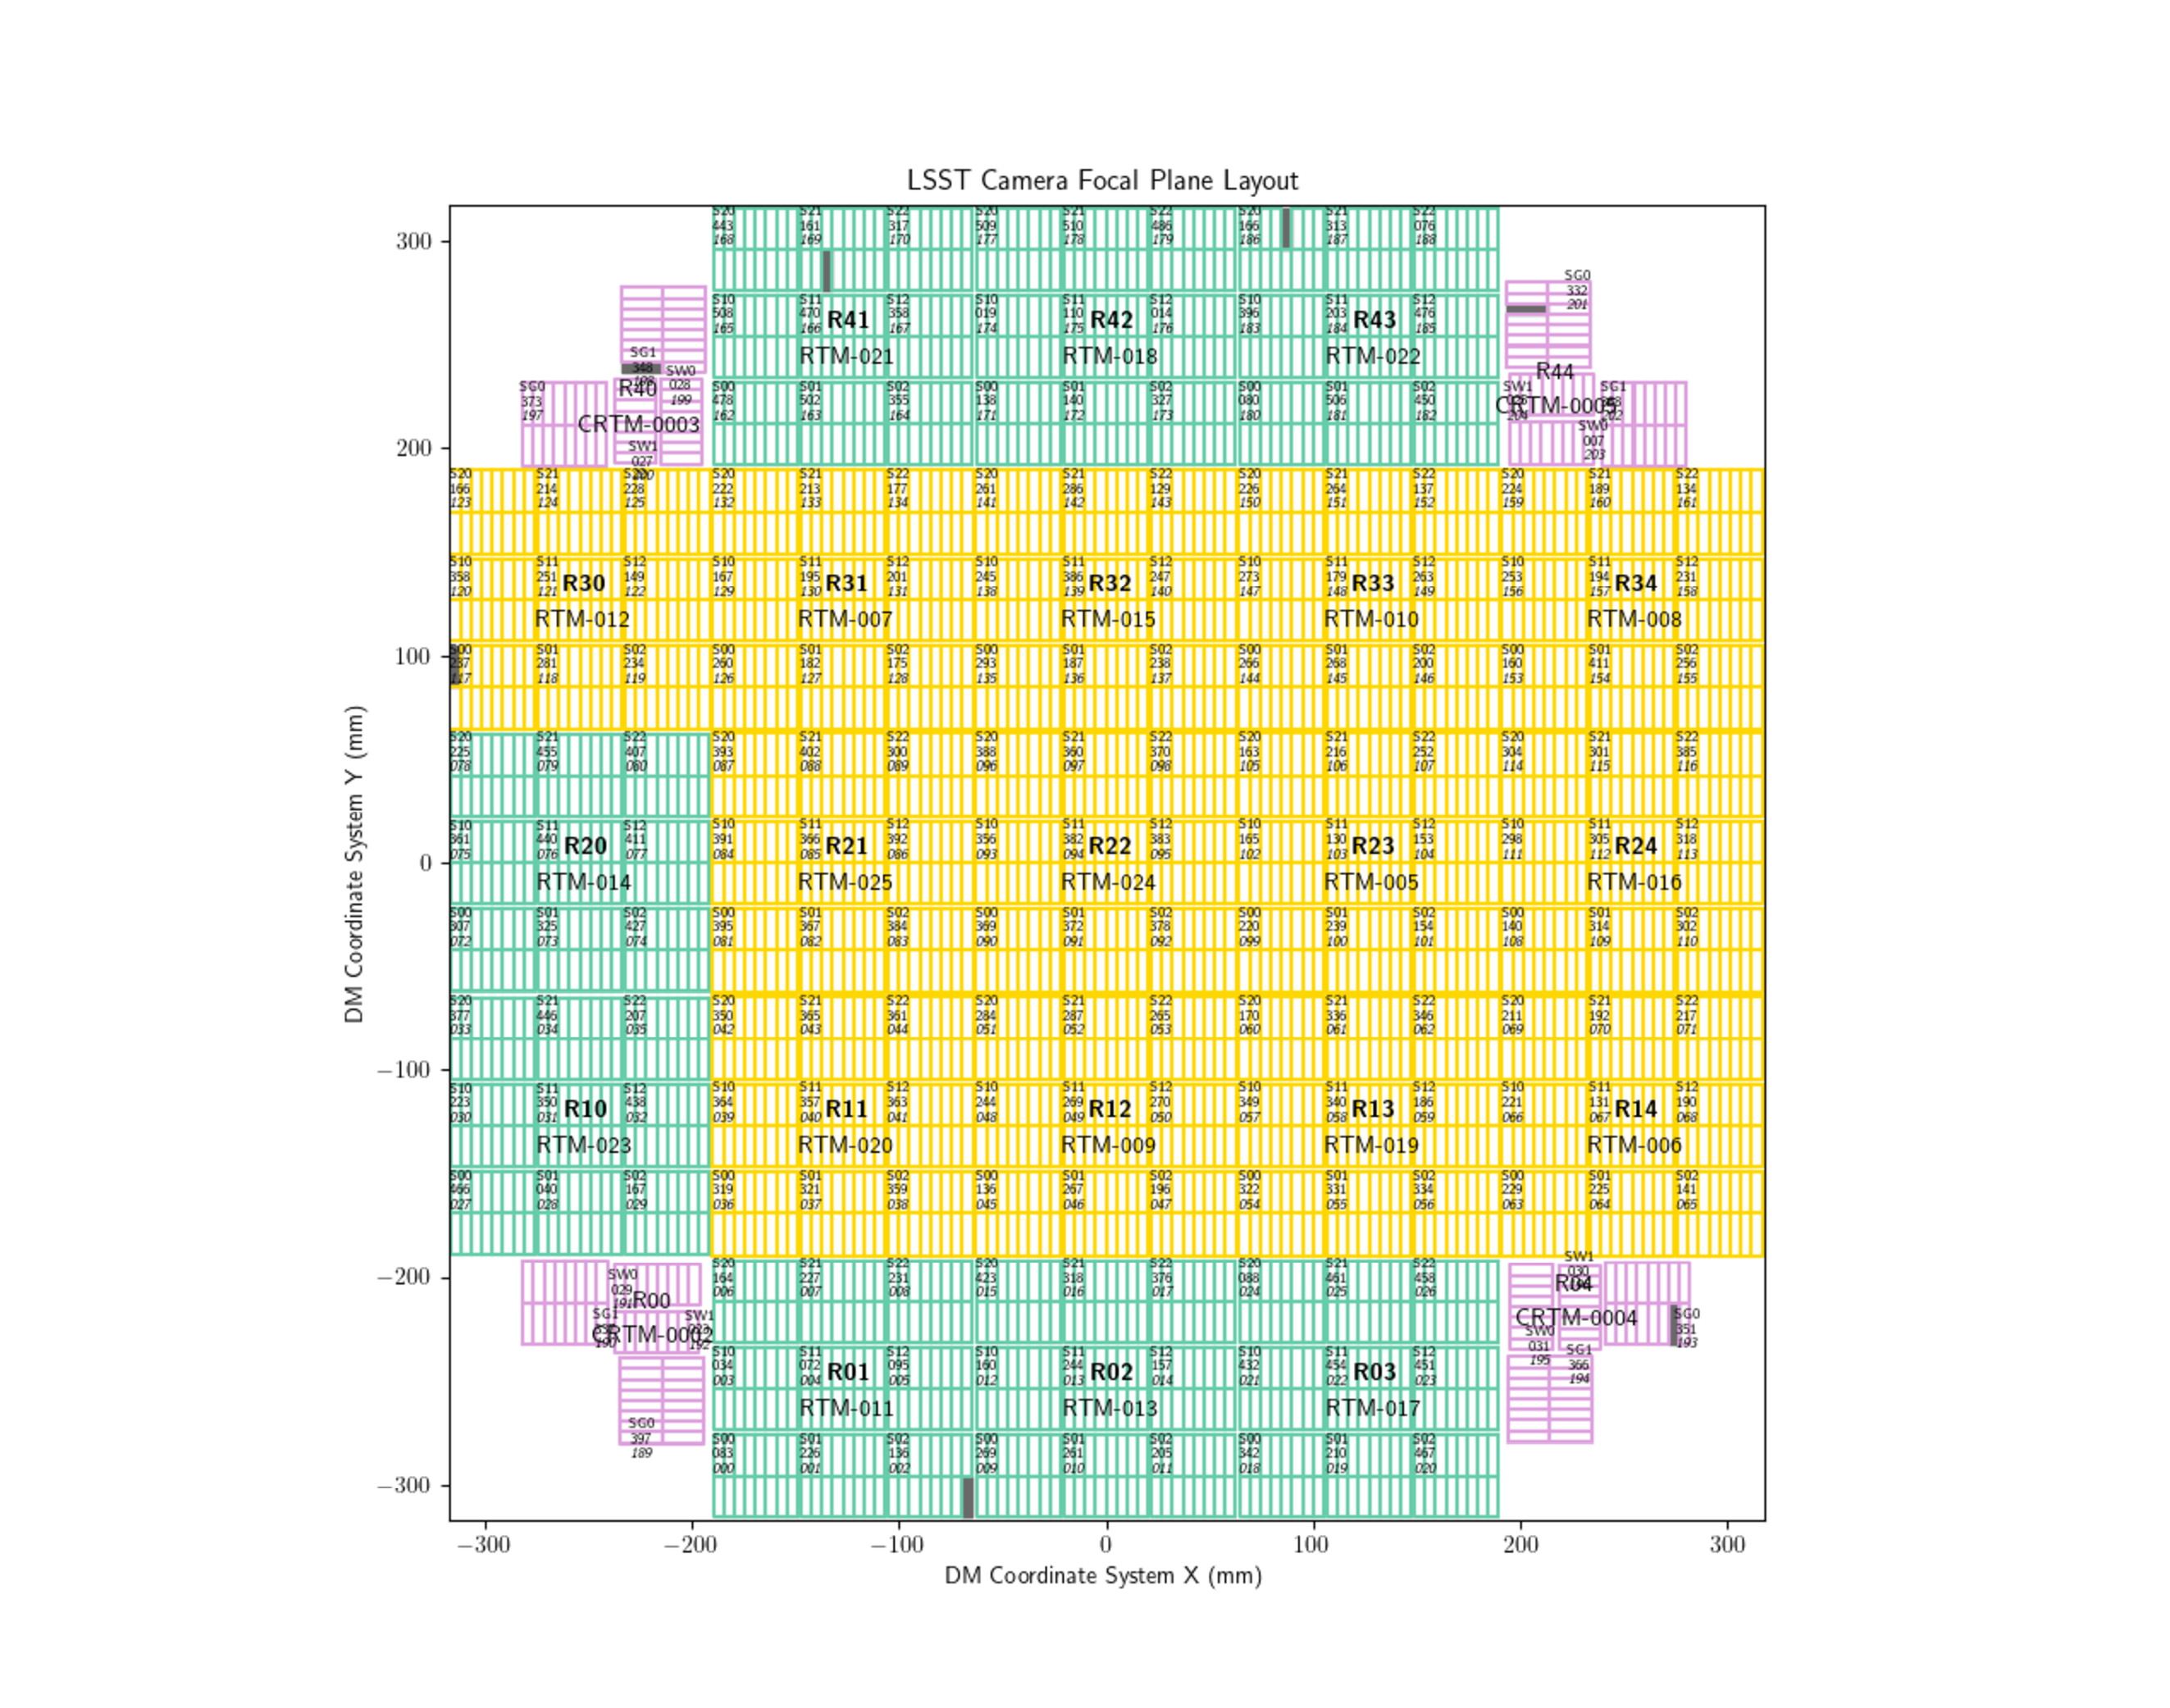
\includegraphics[width=1.0\linewidth]{figures/introduction/LSSTCam_fp_layout_Oct2024.pdf}
    \caption{The focal plane layout}
    \label{fig:focal-plane-layout}
\end{figure}


\subsection{Run 7 optical modifications}\label{run-7-optical-modifications}

For Run 7 in the white room on Level 3 our EO test setup had a few differences from the Run 6 setup in IR2 at SLAC. One difference was that we were not able to use the CCOB Narrow/Thin beam because we did not have the resources to configure it. As
such, the majority of the testing was done with the CCOB Wide Beam
projector\citep{2024SPIE13103E..0WU}. We did obtain an additional projector, the 4K projector, partway through Run 7 that will be discussed later. With the CCOB Wide Beam,
we used a cone attached to the L1 cover as well as a shroud to create a
dark environment (Fig.~\ref{fig:LSSTCam_config}).

\begin{figure}[htbp]
\centering
    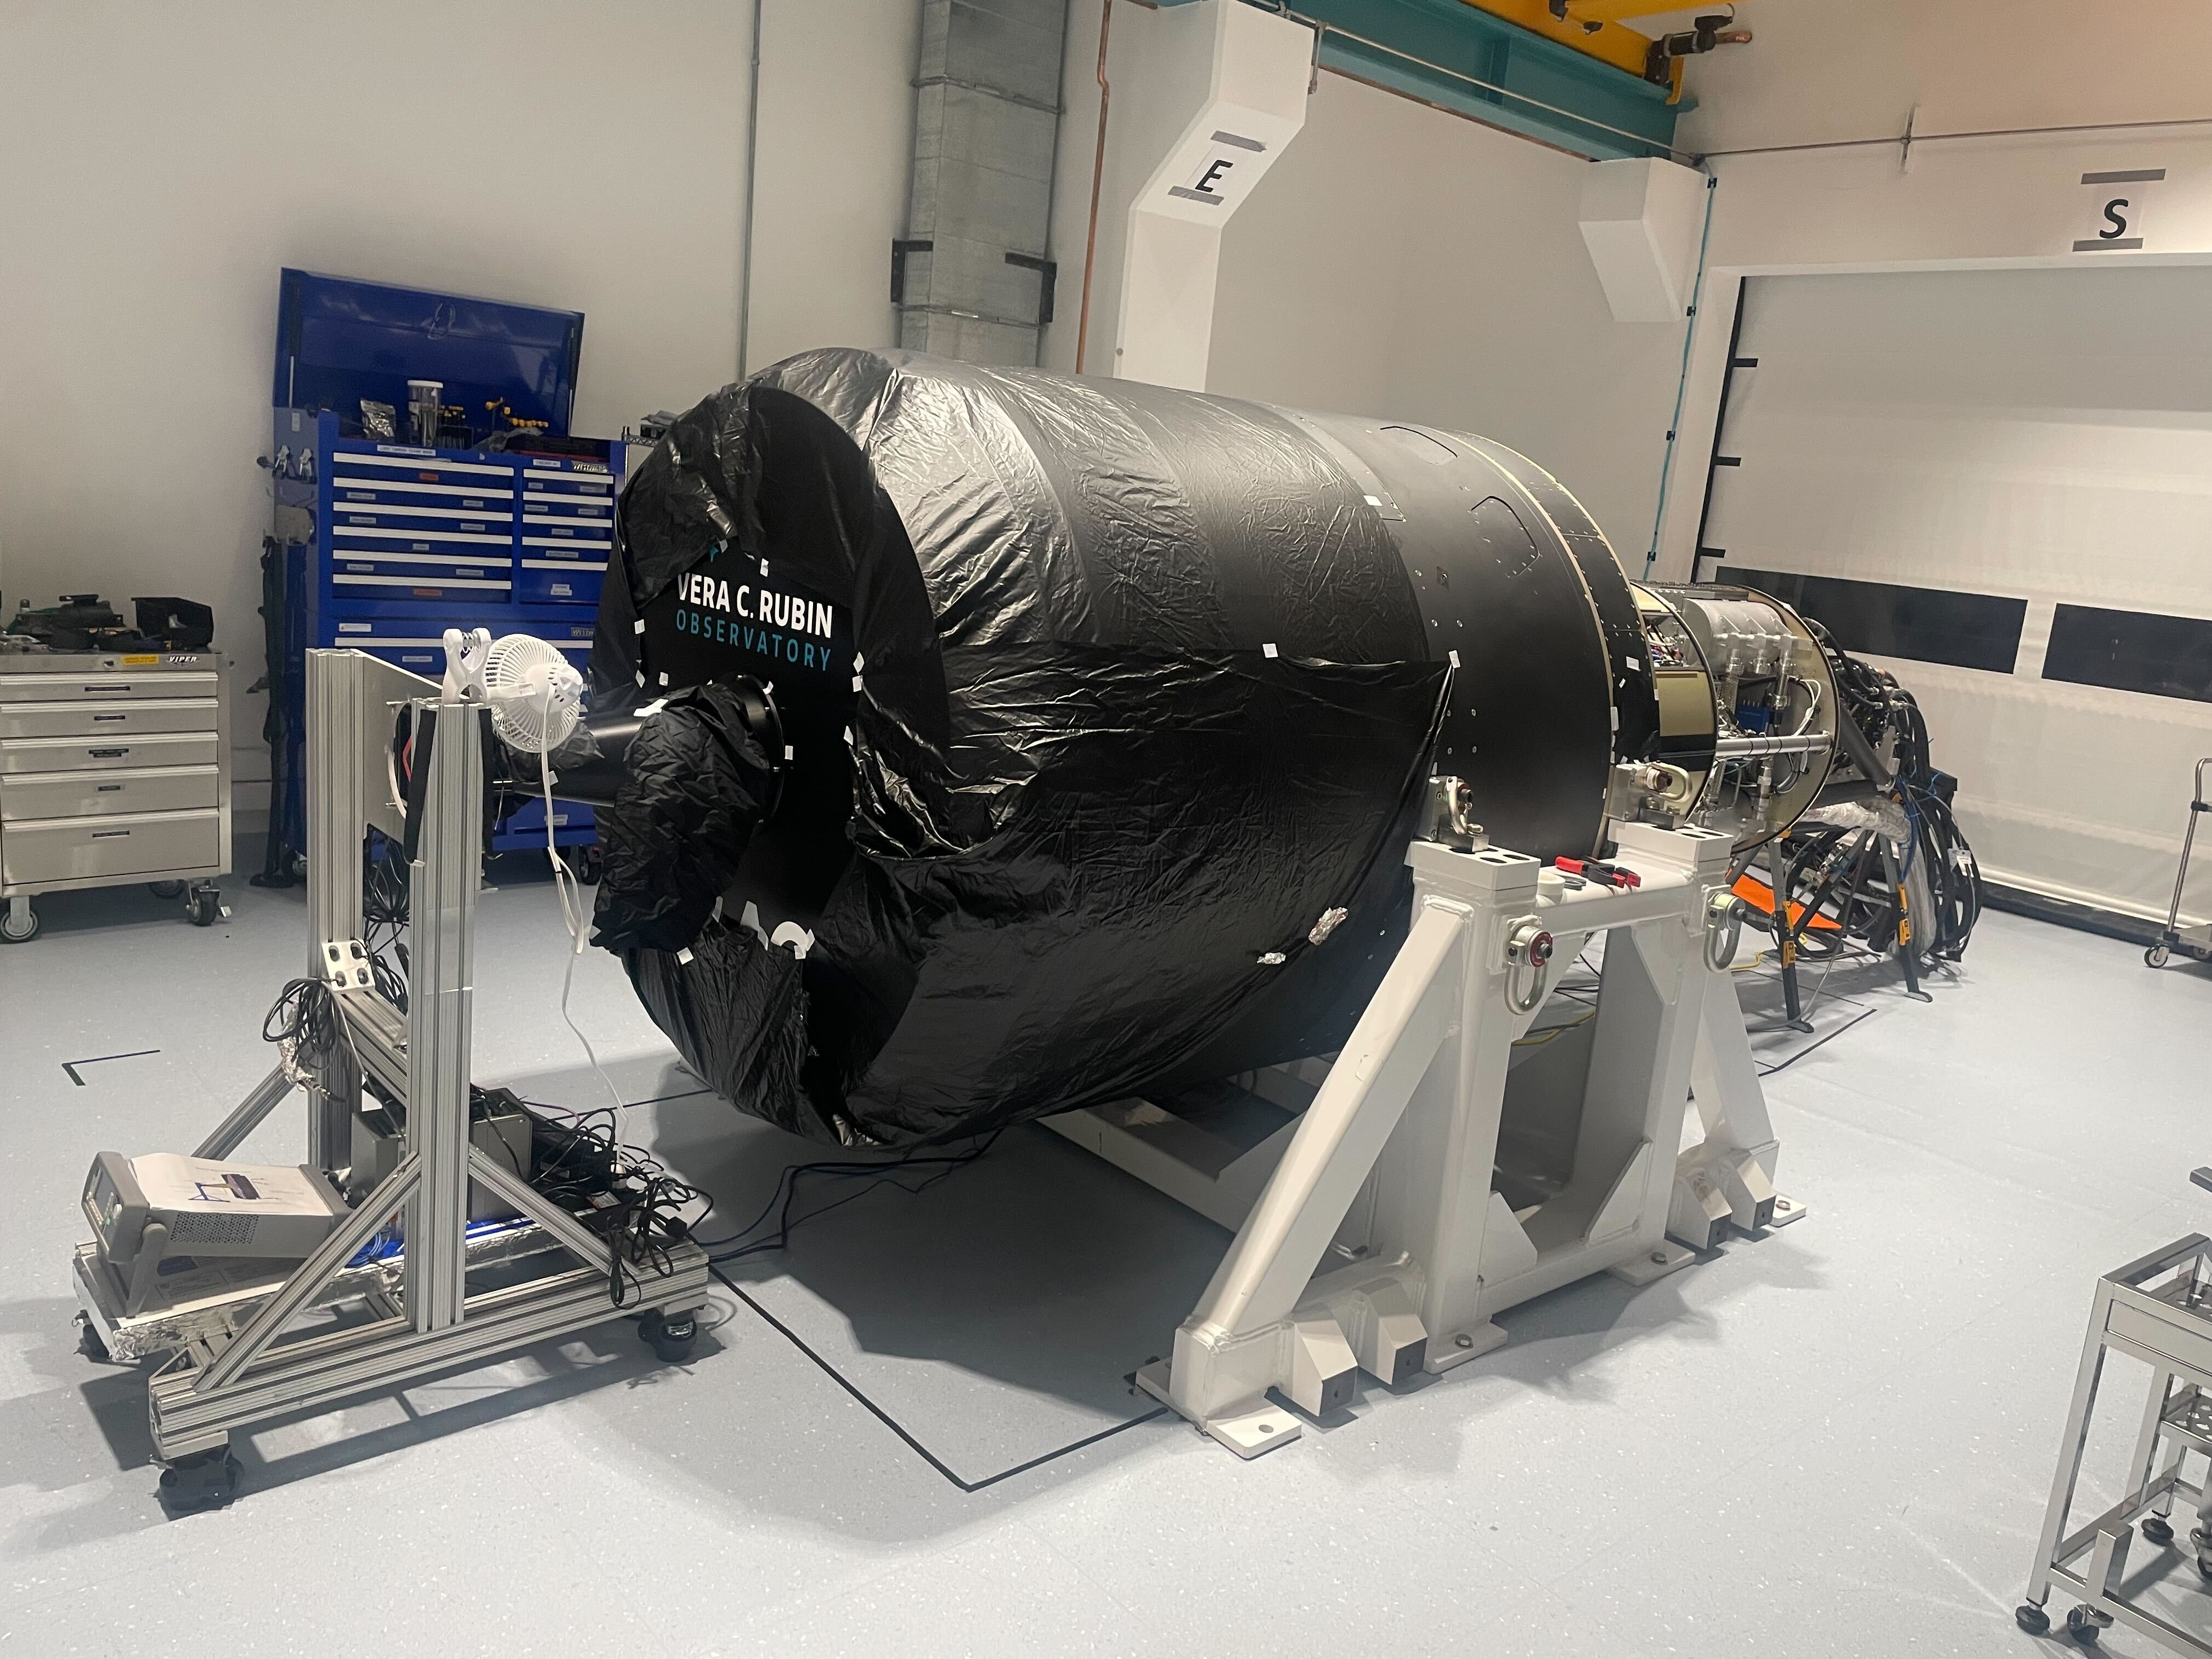
\includegraphics[width=0.6\textwidth]{figures/Camera_Shroud.jpg} 
    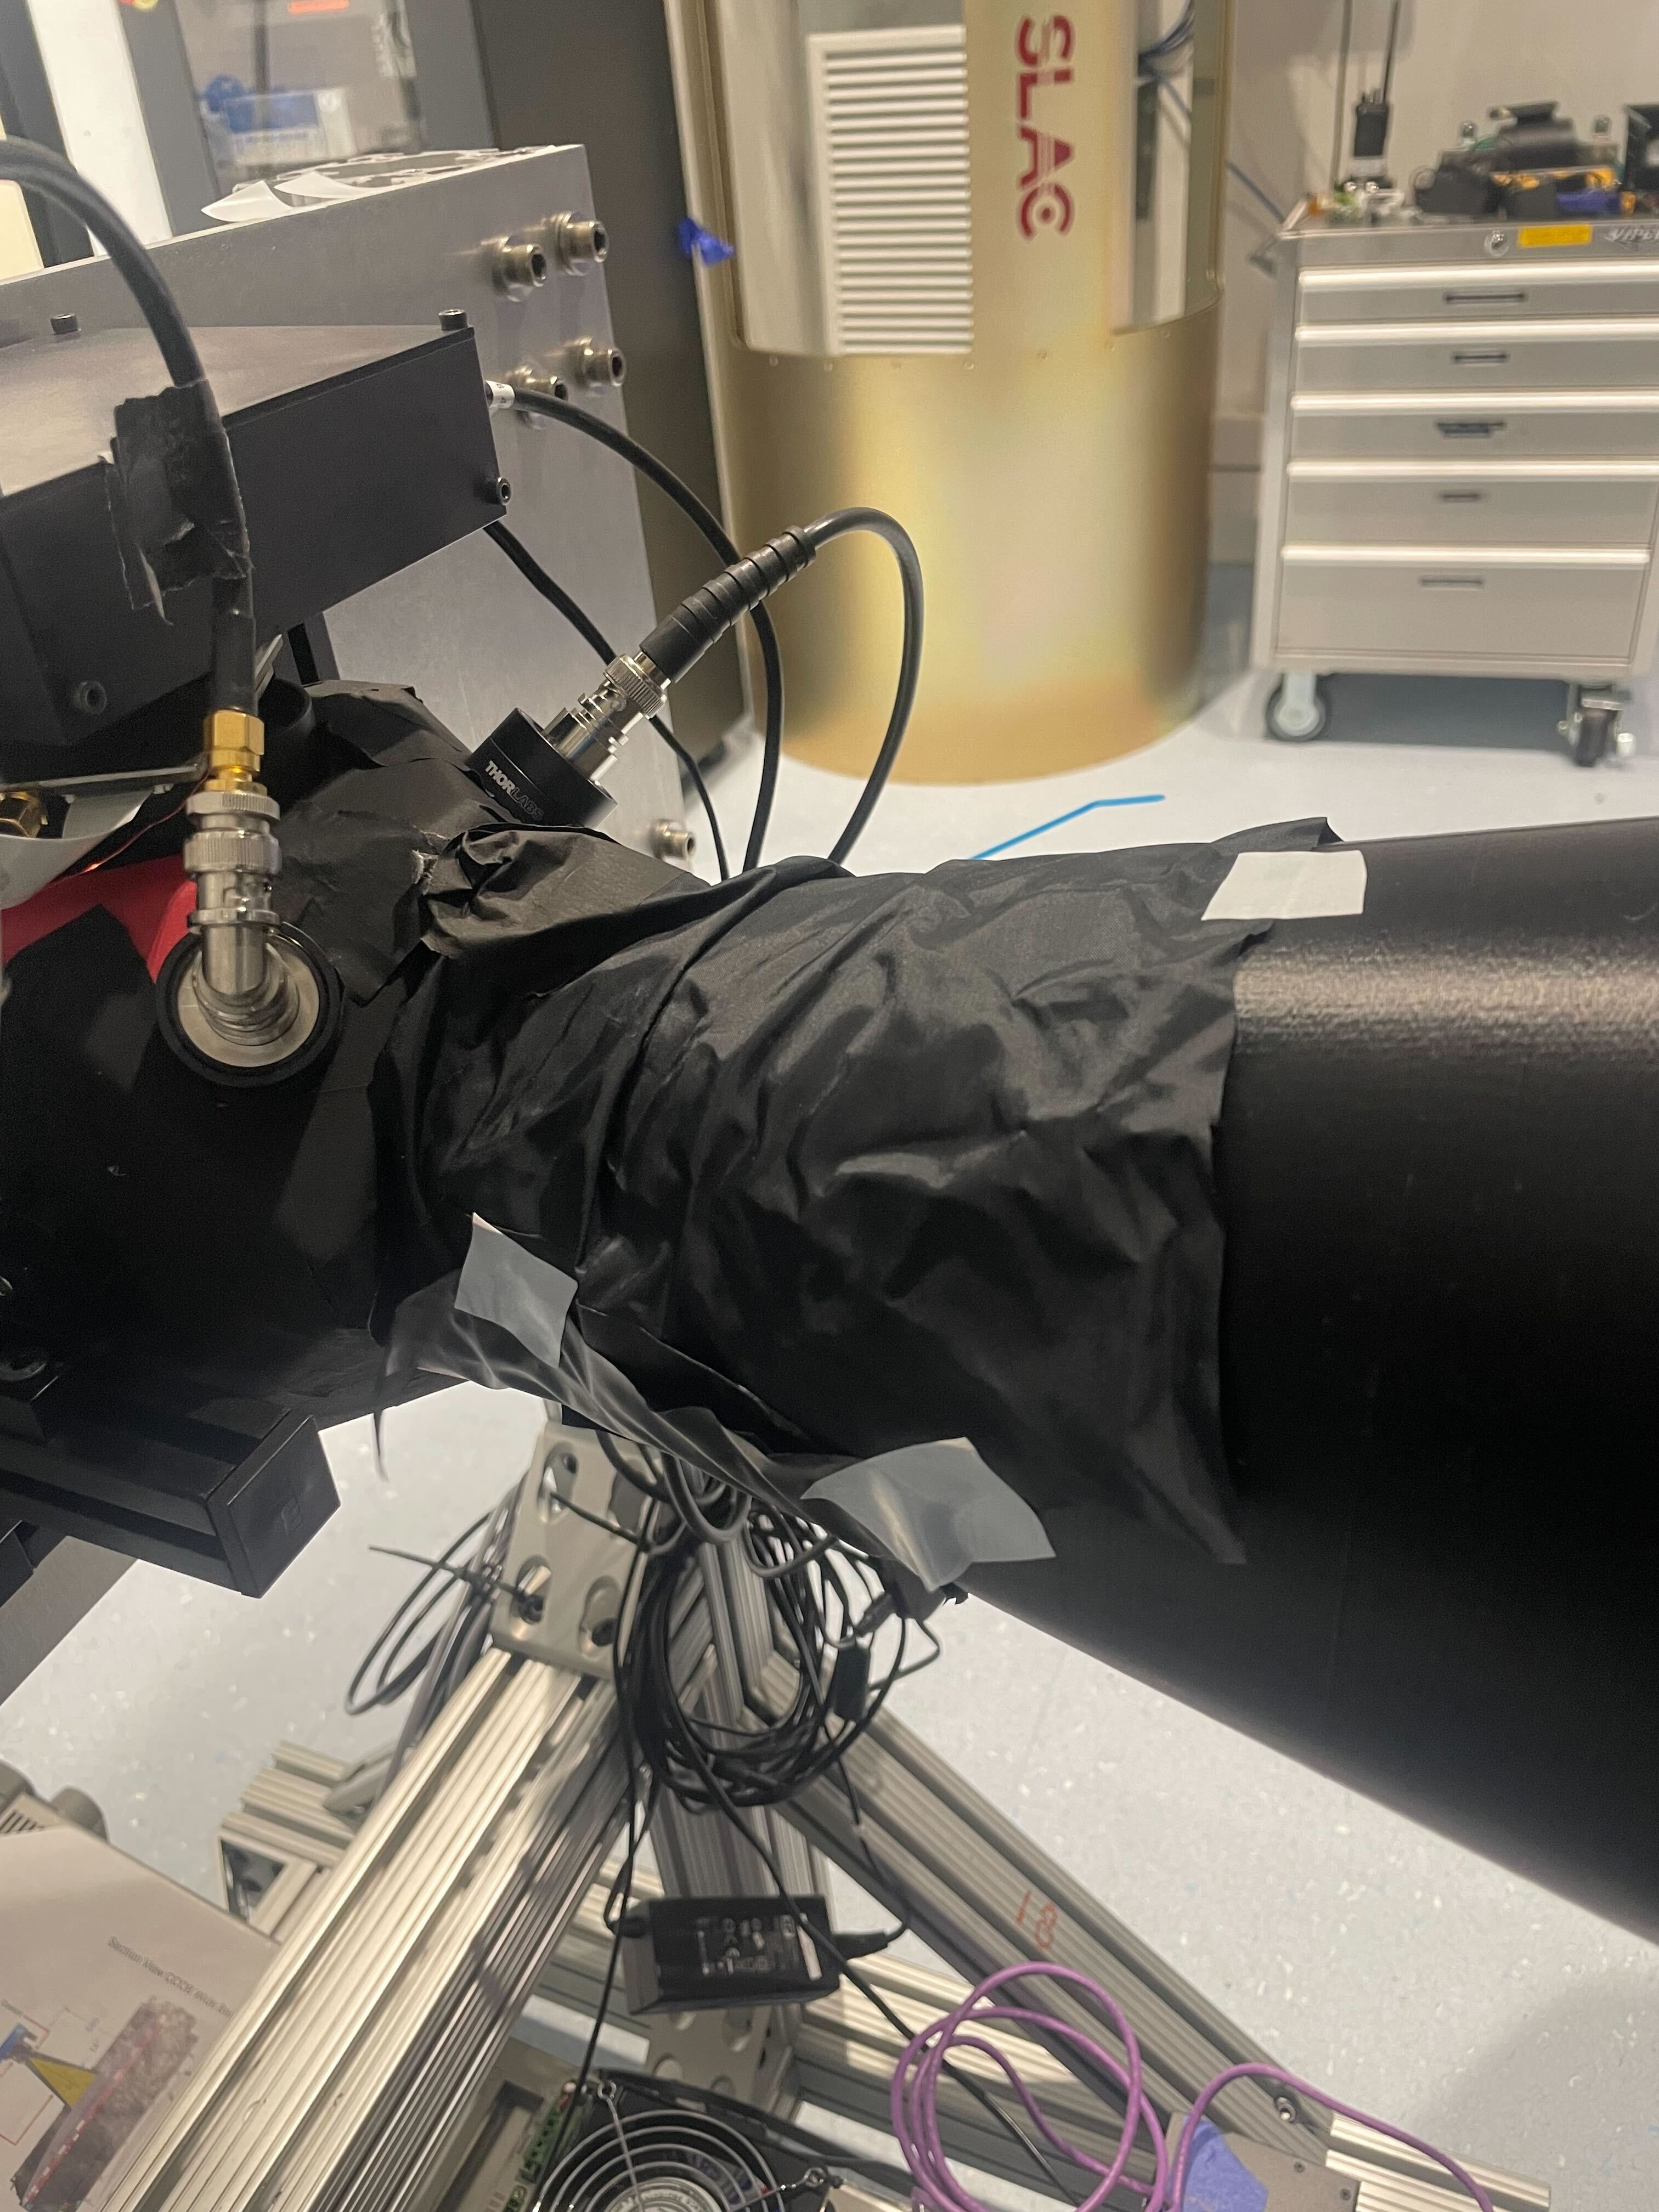
\includegraphics[width=0.35\textwidth]{figures/CCOB_Wide_Shroud.jpg} \\
\caption{(left) Final shroud configuration of LSST Camera in Level 3 to reduce light leaks. (right) CCOB Wide Beam attached to the cone and shrouded.}
\label{fig:LSSTCam_config}
\end{figure}

This allowed us to operate on Level 3 with a dark current of \textless0.1 ADU/sec with the shutter open. The initial setup of the CCOB Wide Beam projector was the same as for Run 6, with a minimal ND filter (10\%) attached to a C-mount lens. One difference was that the f/stop of the lens was changed from 2.6 to 1.6 (fully open). This was done to try to reduce the effect of the `weather' and the `CMB pattern' two effects that we found in Run 6 and were found to be due to our projection setup (see \citet{2024arXiv241113386B}). While changing  the f/stop  did reduce the weather pattern, it also caused a much steeper illumination roll-off across the focal plane (see Figures \ref{fig:roll-off} and \ref{fig:Rolloff_FP}). We evaluated the weather pattern and illumination roll-off relative to Run 6.


To both reduce the effects of the `weather' and `CMB' but retain uniform illumination across the focal plane, we installed a diffuser in the cone attached to L1. Figure~\ref{fig:diffuser} shows the placement of the diffuser within the cone.  The diffuser used is a $60^o$ diffusing angle unmounted sheet from Edmunds Optics.

\begin{figure}[ht]
\centering
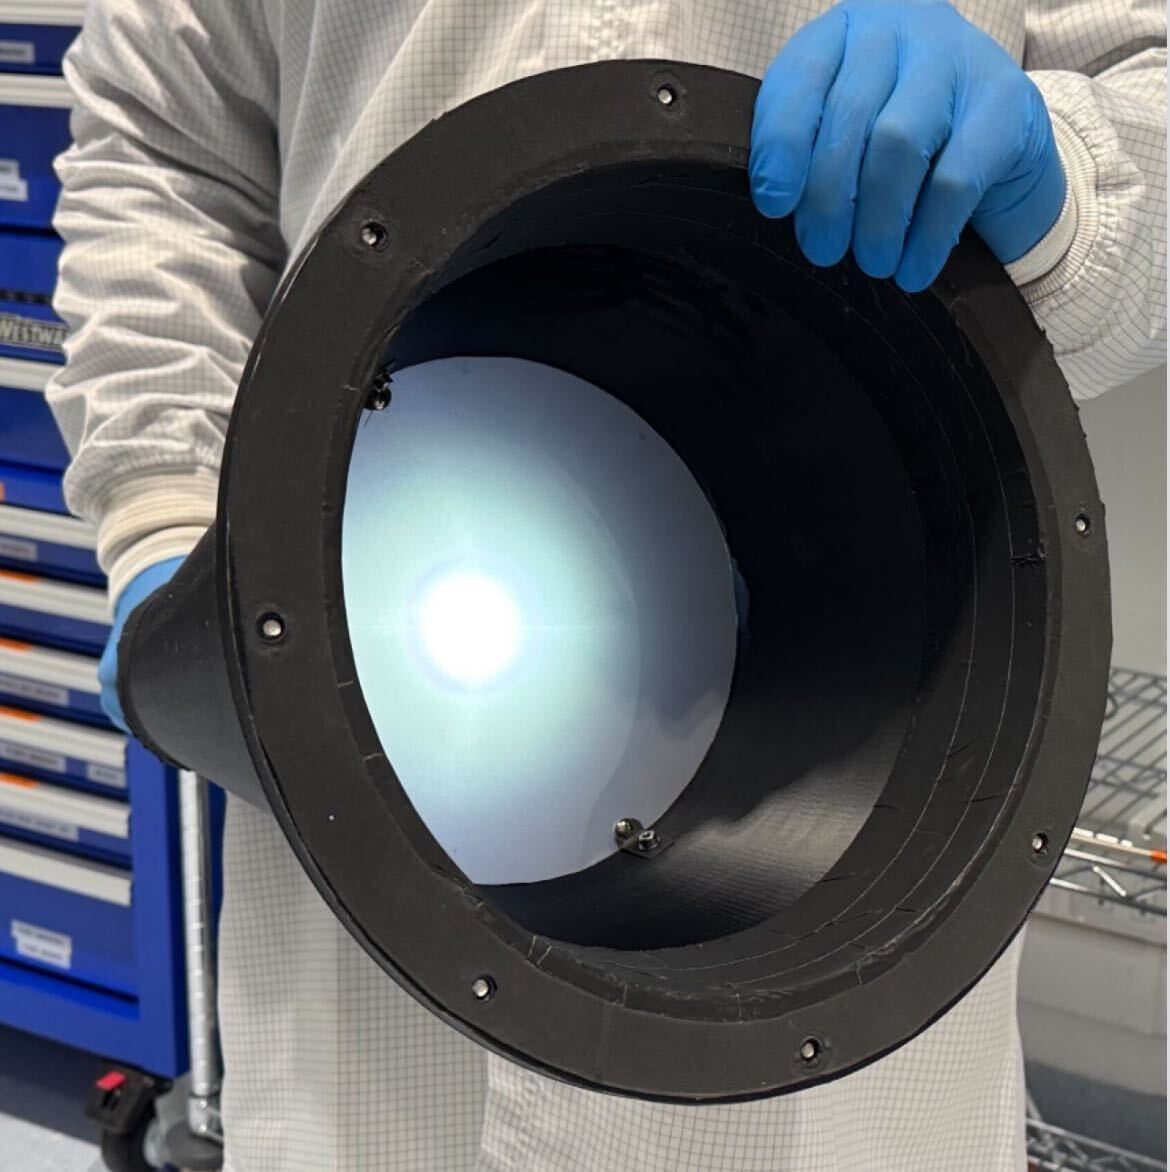
\includegraphics[width=0.6\textwidth]{figures/Diffuser.jpg}
\caption{Diffuser installed into the light cone.}
\label{fig:diffuser}
\end{figure}

We found that the diffuser greatly reduced the `weather' (Fig.~\ref{fig:weather}) and eliminated the CMB pattern and more uniformly illuminated the focal plane (Fig.~\ref{fig:roll-off}), and removed the extreme roll-off (Fig. \ref{fig:roll-off} and Fig. \ref{fig:Rolloff_FP}) with a penalty of decreasing the overall illumination by roughly 35\% even though we fully opened the f-stop.


\begin{figure}[htbp]
\centering
\begin{minipage}{0.45\textwidth}
    \centering
    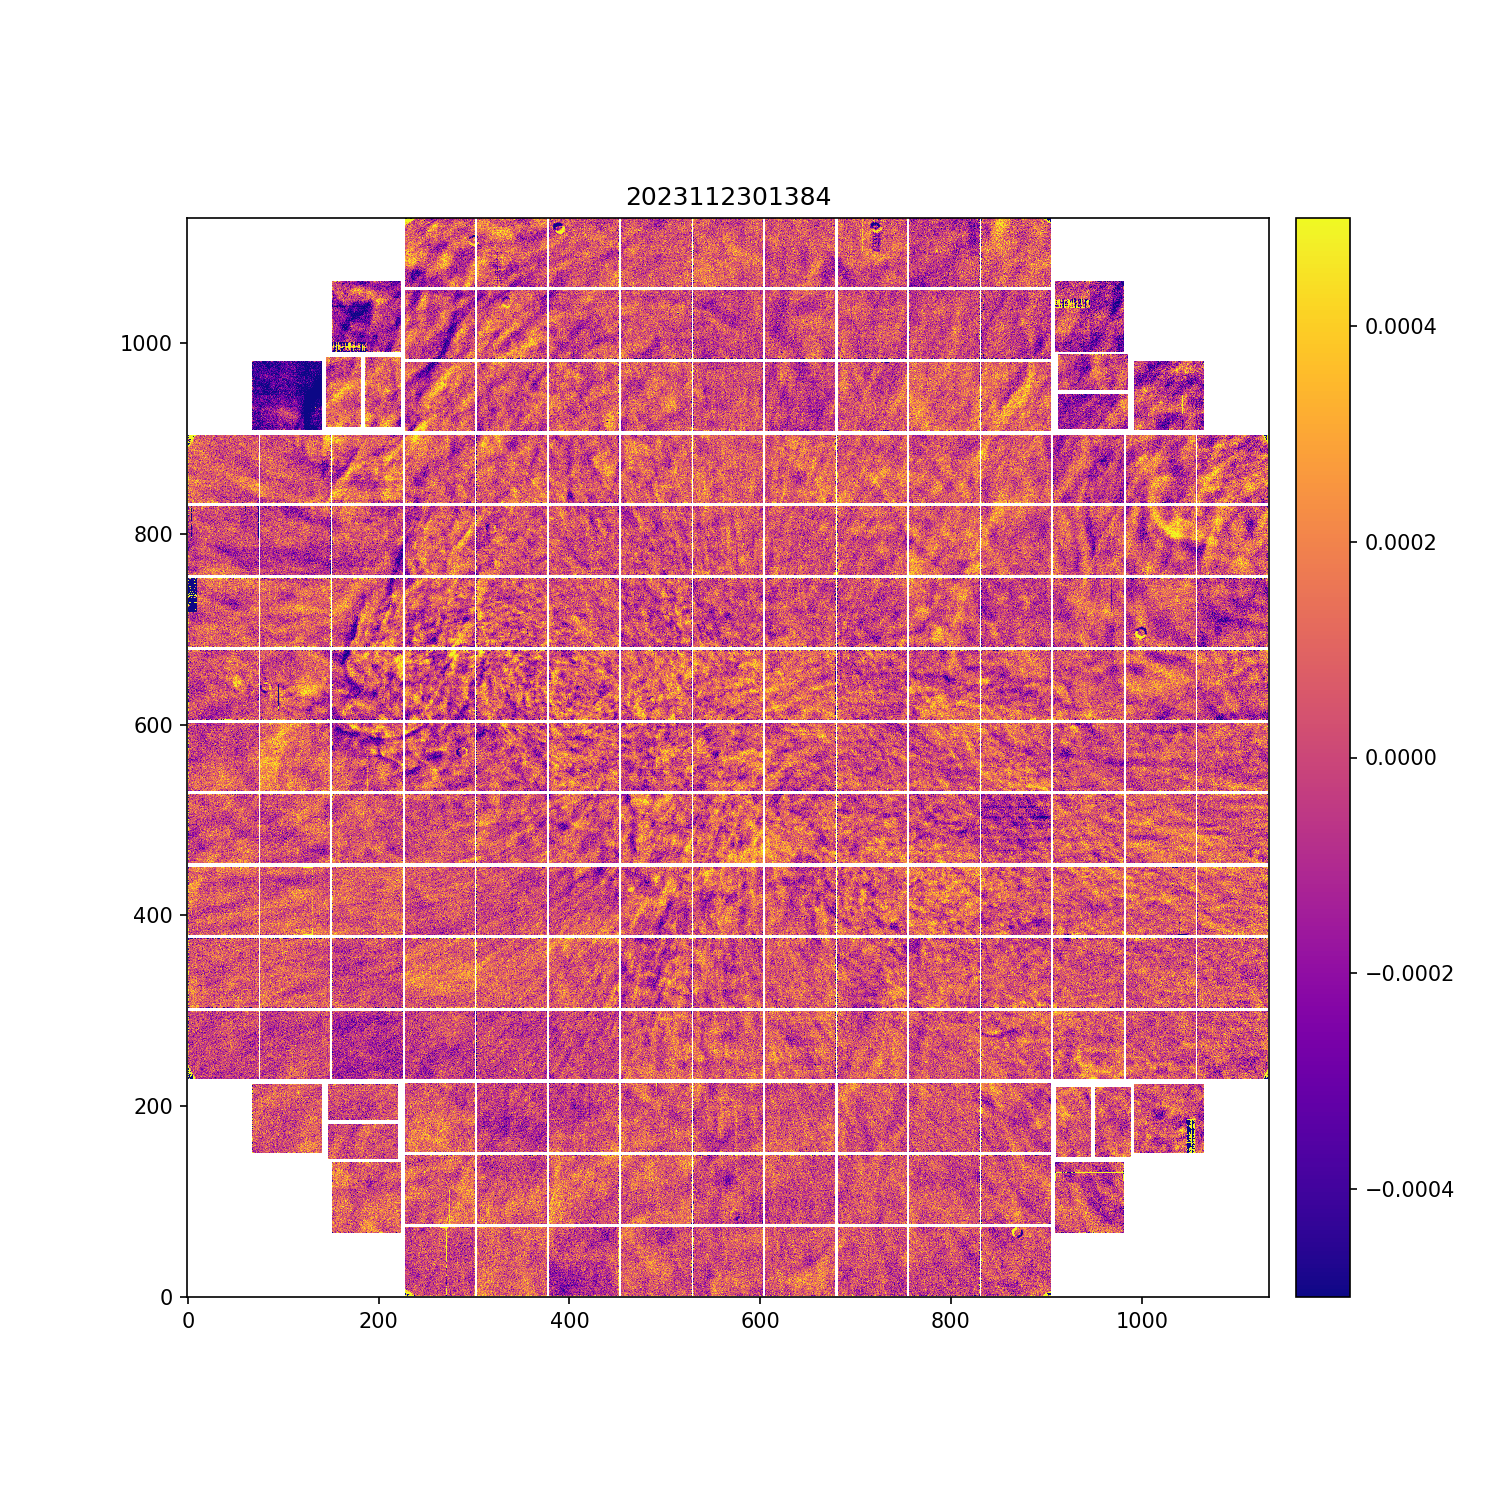
\includegraphics[width=\linewidth]{figures/Run6_Weather.png}
%    \caption{Full focal plane image showing the fractional difference in Run 6.}
\end{minipage}
%\hfill
\begin{minipage}{0.5\textwidth}
    \centering
    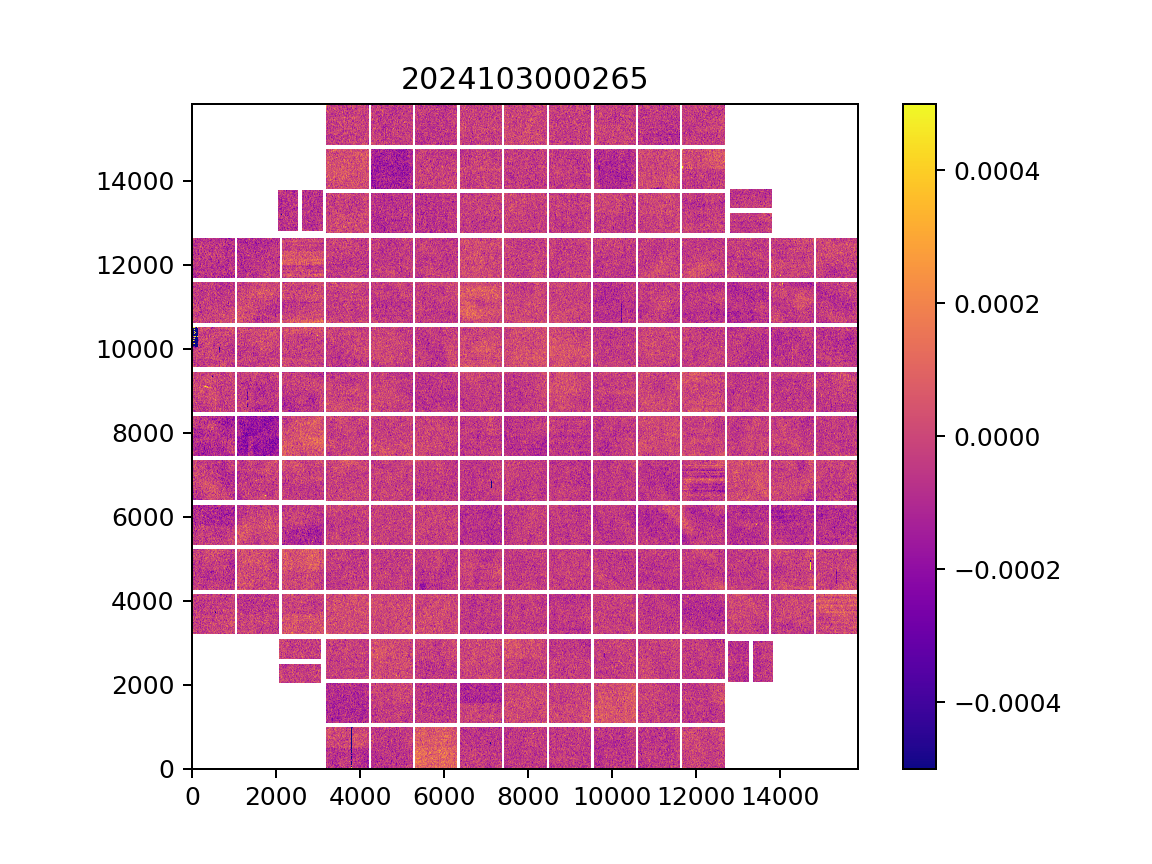
\includegraphics[width=\linewidth]{figures/Run7_WeatherDiffuser.png}
\end{minipage}    
    \caption{Full focal plane fractional difference of images for Run 6 (left) and Run 7 (right).}

\label{fig:weather}
\end{figure}

\begin{figure}[htbp]
\centering
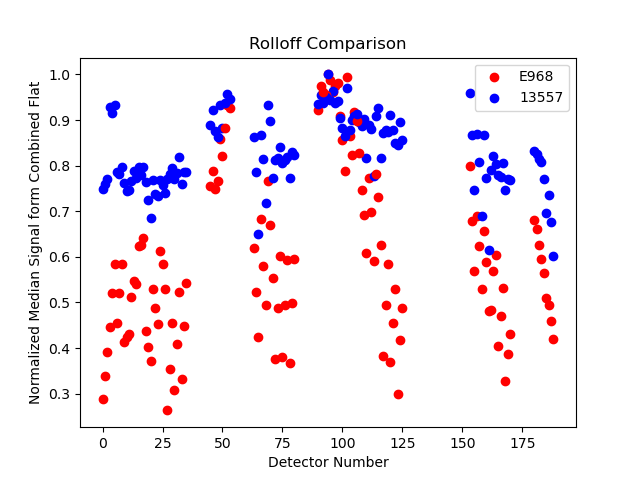
\includegraphics[width=0.48\textwidth]{figures/Run7_Illumination.png}
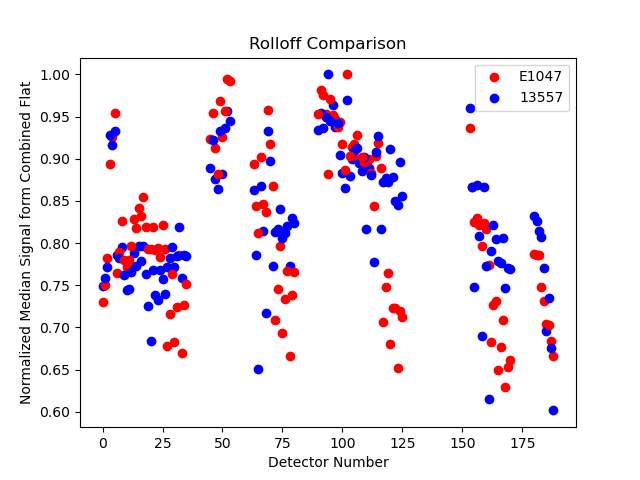
\includegraphics[width=0.48\textwidth]{figures/Run7_DiffuserIllumination.png}
\caption{(left) Illumination across the focal plane from Run 7 without the diffuser (E968) as compared to Run 6. (right) Illumination across the focal plane from Run 7 with the diffuser (E1047) as compared to Run 6.}
\label{fig:roll-off}
\end{figure}

\begin{figure}[ht]
    \centering
    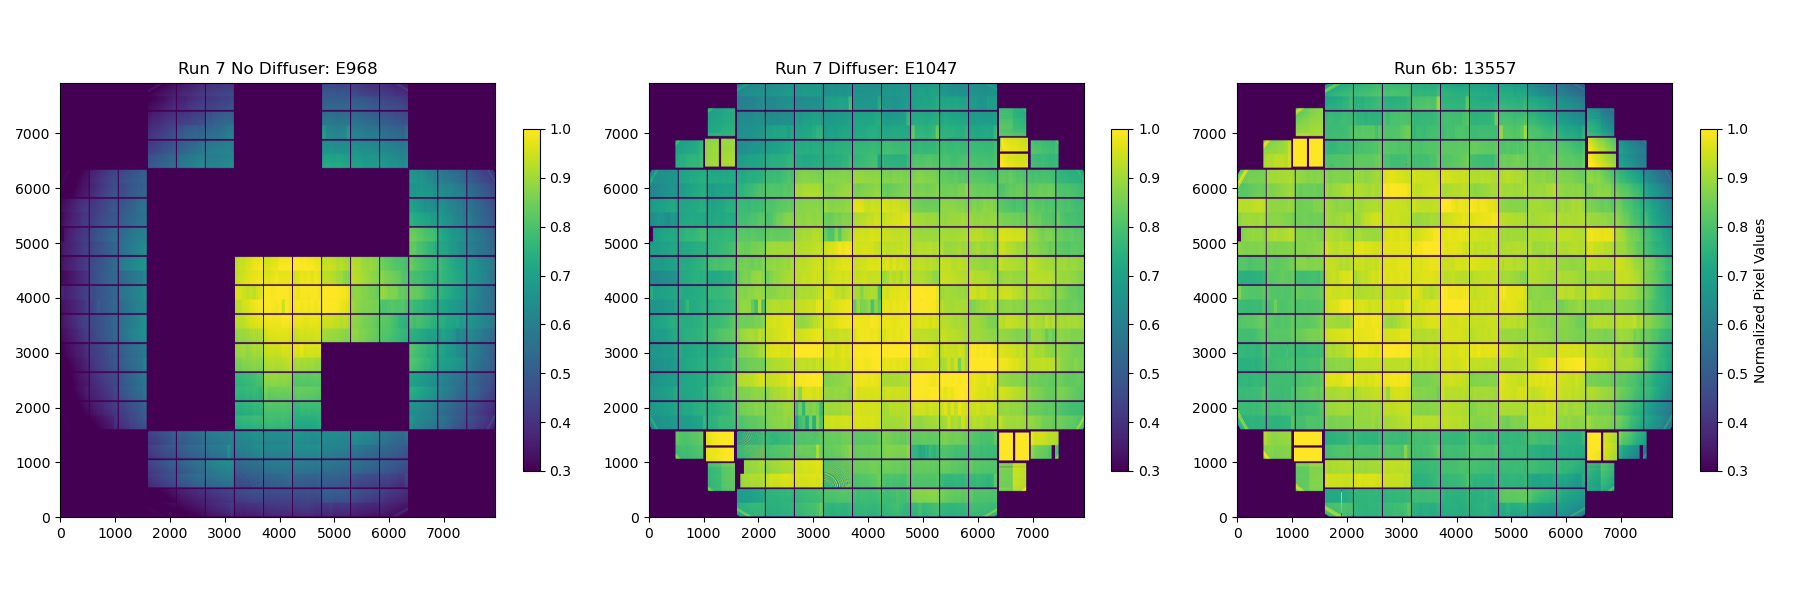
\includegraphics[width=0.95\linewidth]{figures/Rolloff_FP.png}
    \caption{Combined flat images from three different runs that show the roll-off of the CCOB Wide Beam with Run 7 data without the diffuser and with the projector aperture open (left), Run 7 data with the diffuser and projector aperture closed (middle), and Run 6 without the diffuser but the projector aperture closed (right). The pixels are normalized and the left figure is missing detectors as we were still in the process turning them off when doing this test.}
    \label{fig:Rolloff_FP}
\end{figure}


The diffuser was installed for all B protocol and PTC runs (see Sec. \ref{sec:reverification}) moving forward, being taken out only for pinhole projection runs and when using the 4K projector.

\subsection{Projector spots}\label{projector-spots}
The addition to the projectors used for EO testing was a 4K projector (Epson LS11000 LCD), similar to those used in conference rooms. This projector was first tested at SLAC and arrived at the observatory about halfway through Run 7. It was used primarily as a spot projector, as the pinhole filter was not available at that time because of the Filter Exchange System was temporarily inoperable. The projector has an advantage, instead, as it could illuminate all 3206 amplifiers instead of just the 21 illuminated by the
pinhole projector. Figure \ref{fig:SpotProjector_L3_FP} shows both the setup of the projector on Level 3 and an example of a spot image and the spots across the focal plane. Since the projector does not have fast illumination control, we primarily used the LSST camera main shutter instead of any flashing of the light source (e.g., as we did with the LEDs of the CCOB Wide Beam). One downside that was found was that the projector illuminated the entire focal plane at some background level, not just the spot regions. The background illumination also had structure that changed with time and could not be easily subtracted. Figure \ref{fig:SpotProjector_Spots} shows an example of a spot image of just one detector as well as a zoomed in image of a single spot which highlights the background structure. The resulting contrast between the spot and the background was only about a factor of 6. Changing the spot shape to large rectangles for crosstalk
measurements increased the contrast ratio to 30. Examples of the rectangles can be seen in Figure \ref{fig:SpotProjector_Rect}. Though the contrast was much improved, there was still a background structure as can be seen in the saturated image of the figure.

\begin{figure}[htbp]
\centering
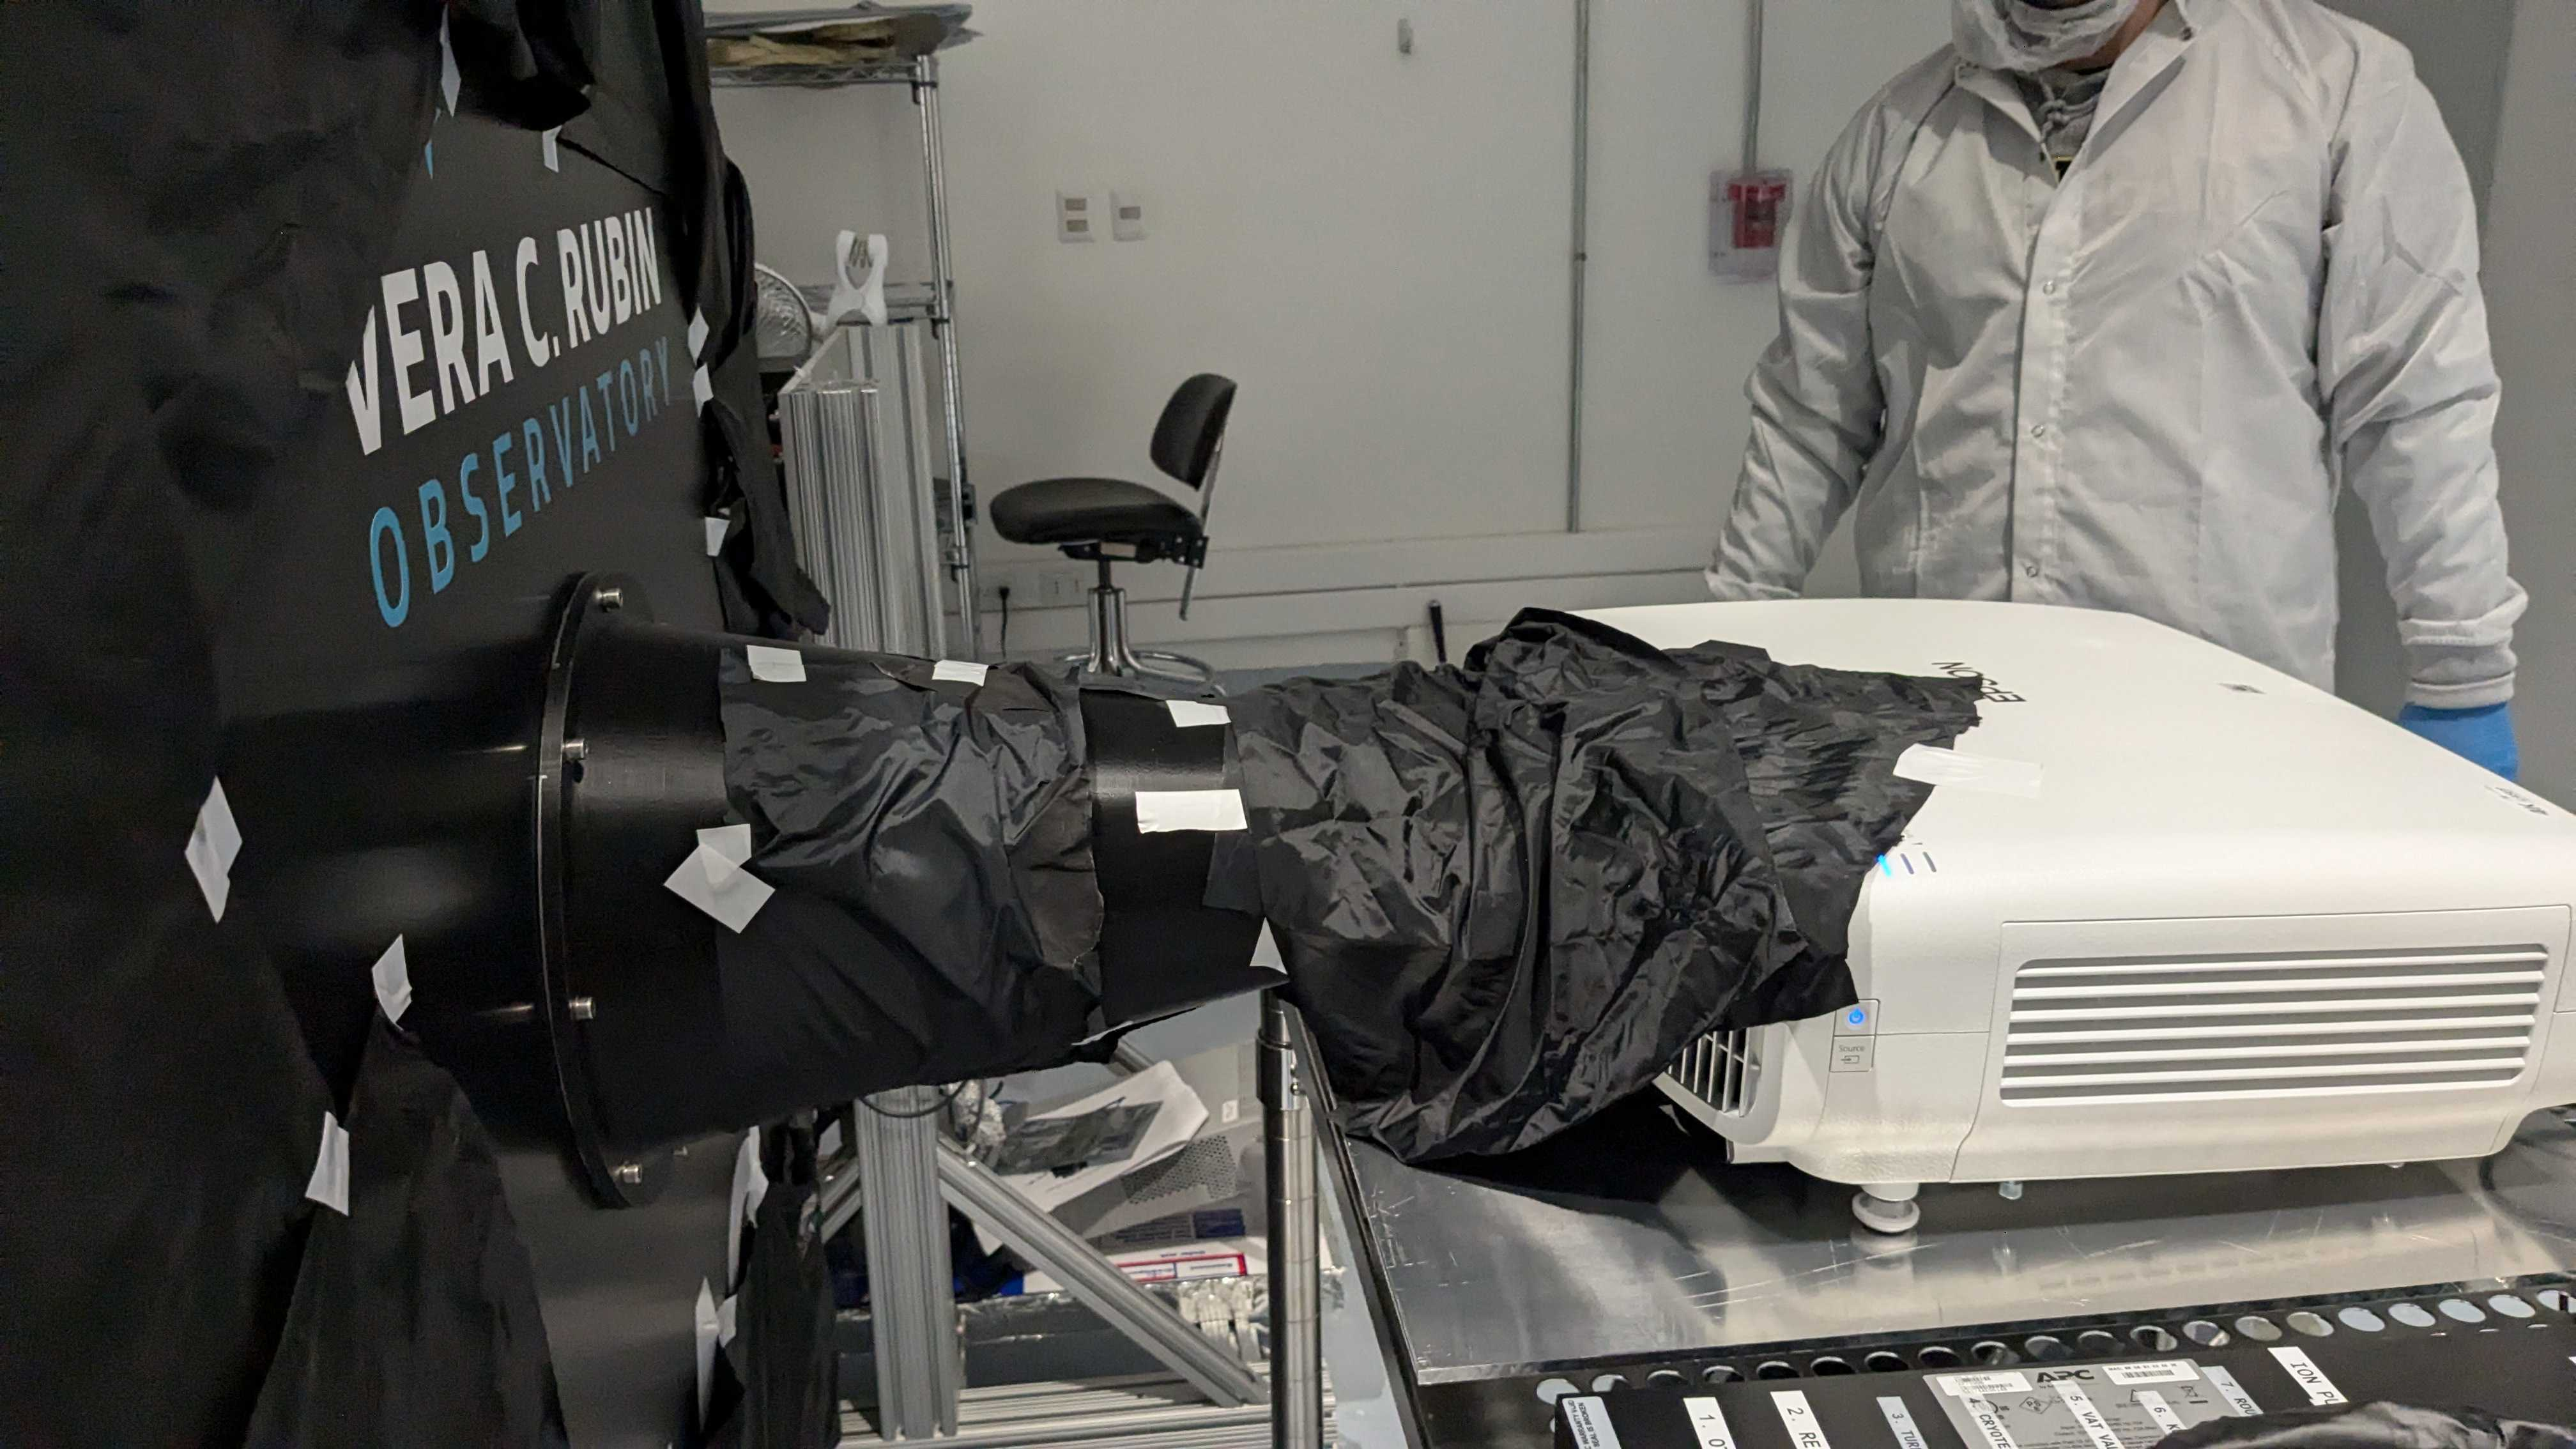
\includegraphics[width=0.48\textwidth]{figures/SpotProjector_Level3.jpg}
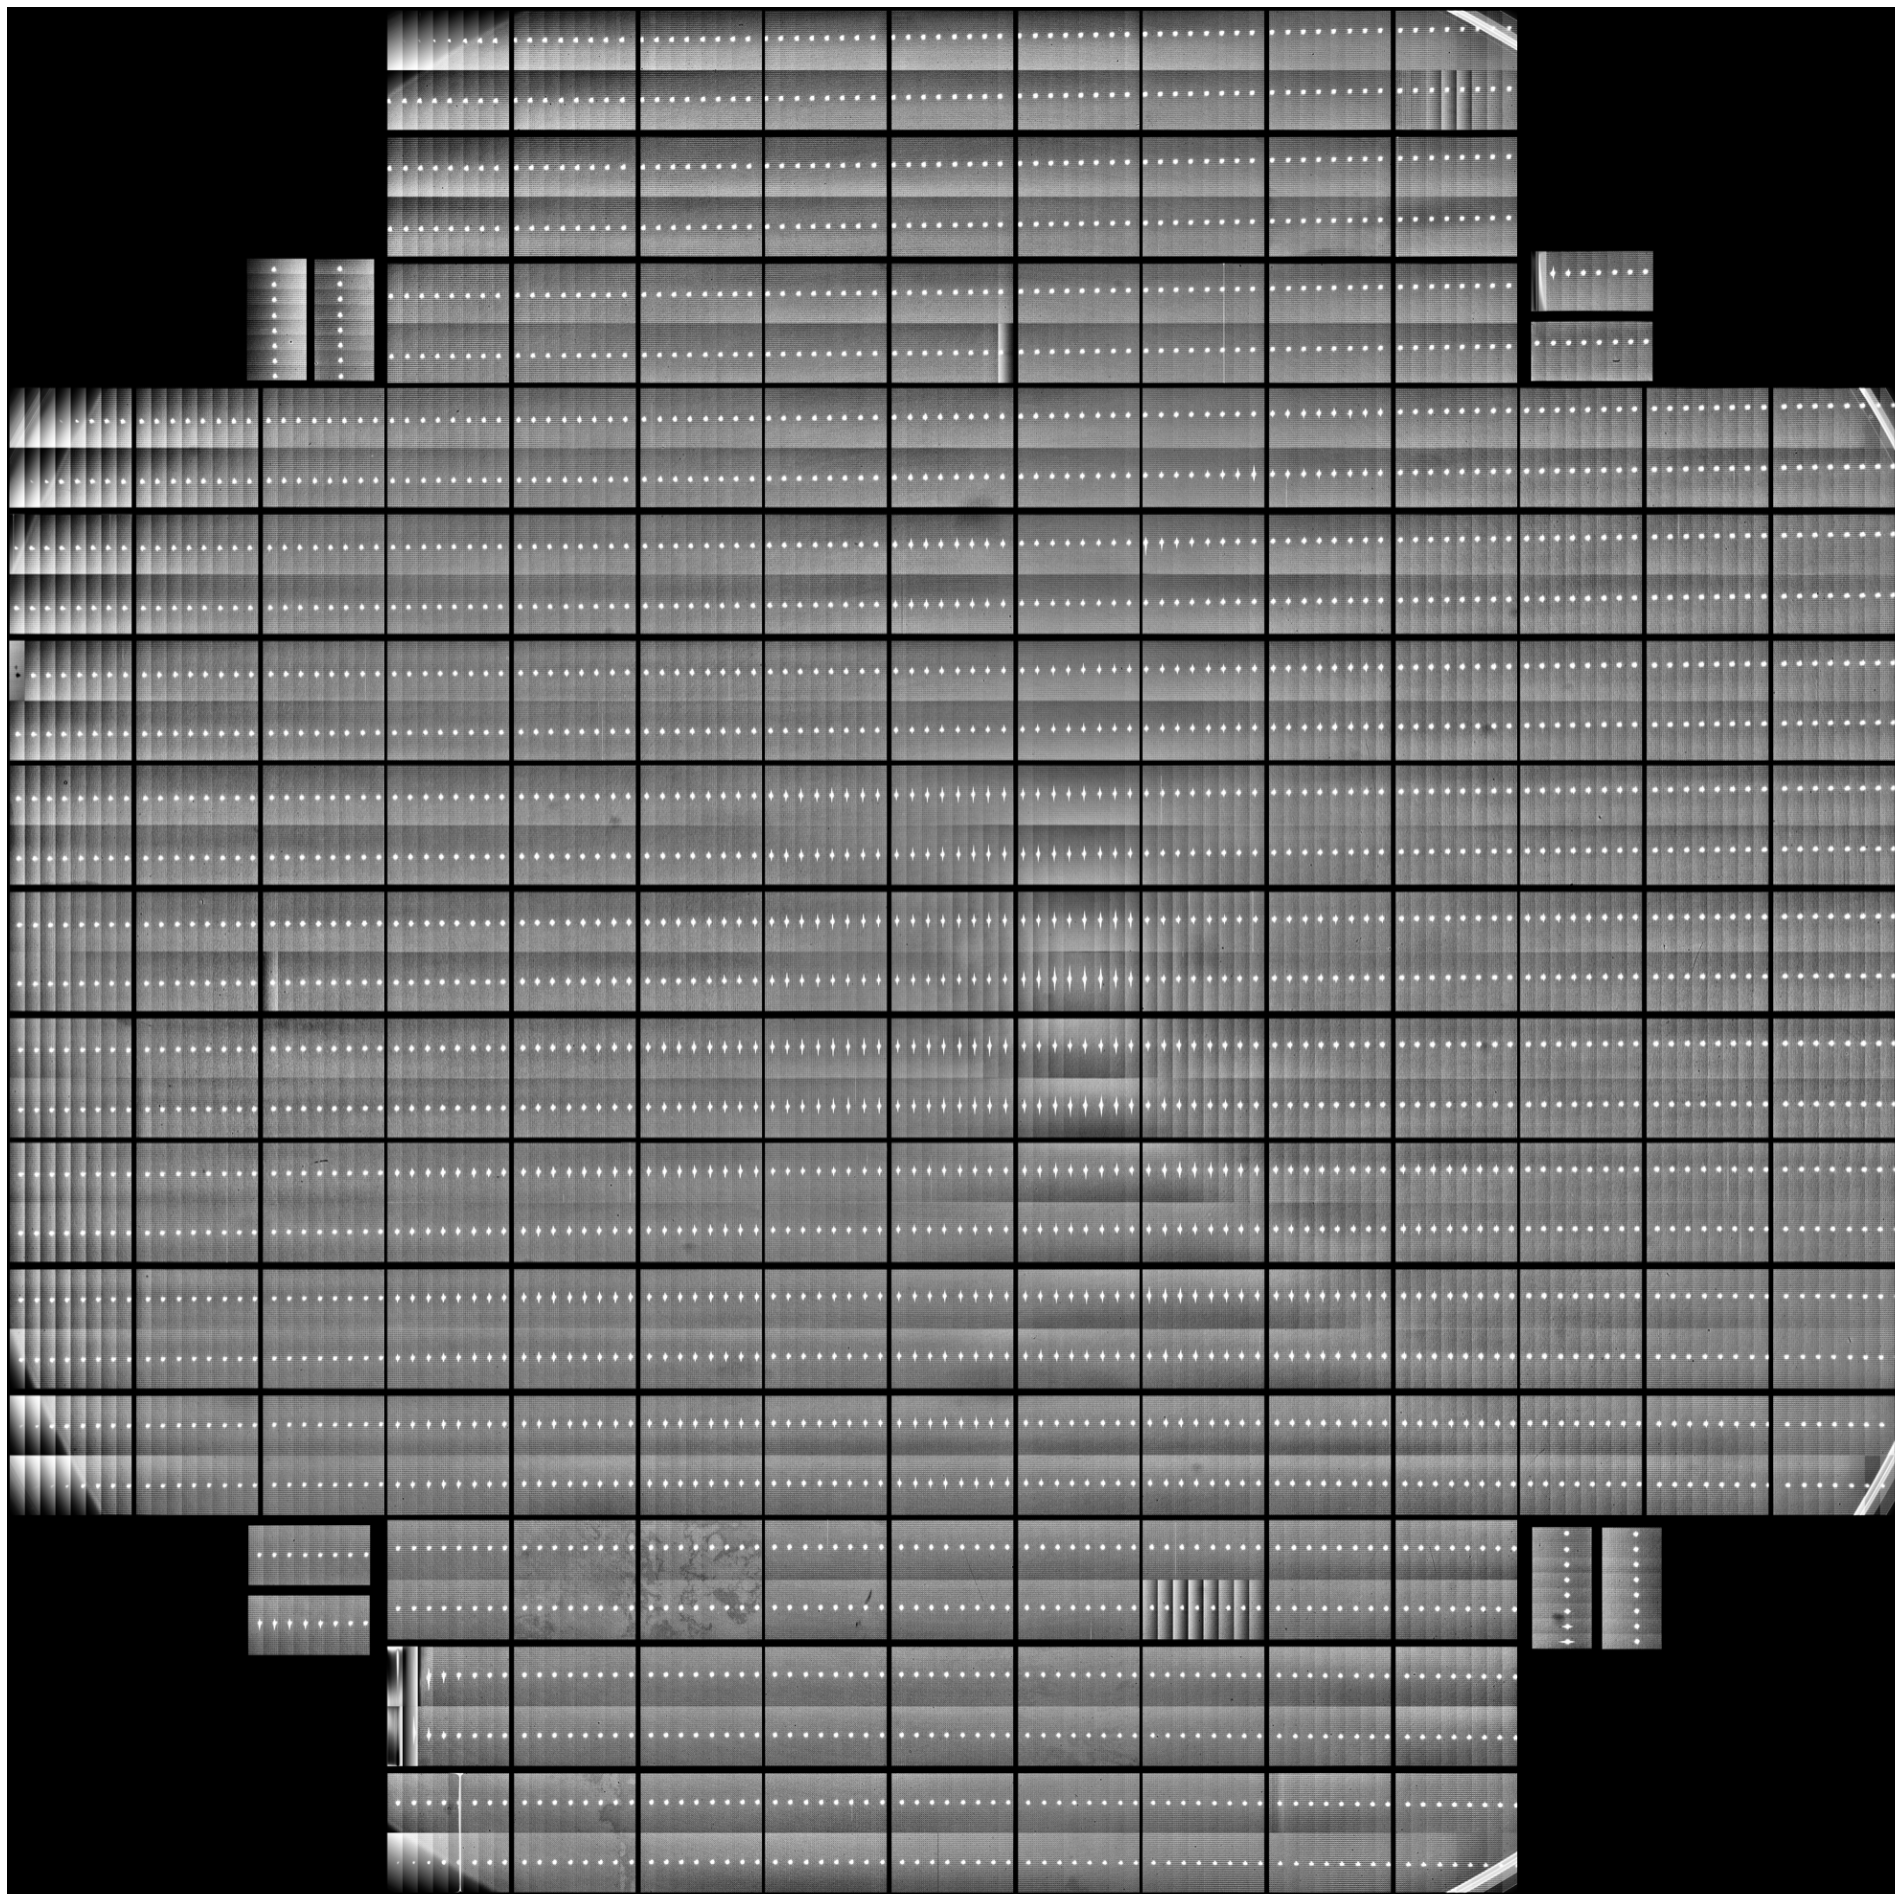
\includegraphics[width=0.48\textwidth]{figures/SpotProjector_FP.png}
\caption{(left) The spot projector set up on Level 3. (right) An example of an image taken with the spot projector with all the amplifiers containing a spot.}
\label{fig:SpotProjector_L3_FP}
\end{figure}

\begin{figure}[htbp]
\centering
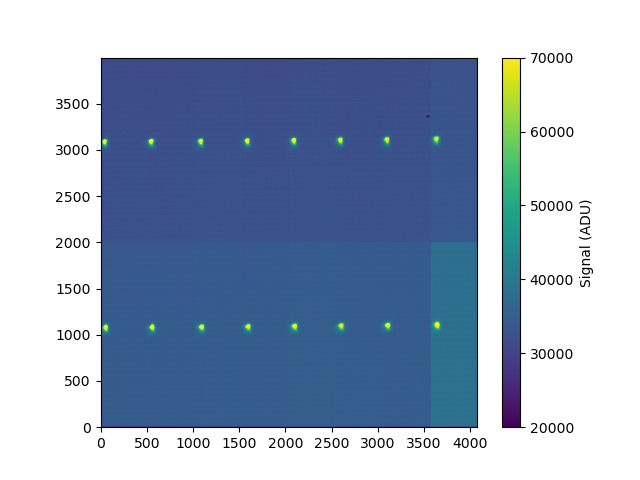
\includegraphics[width=0.48\textwidth]{figures/Spot_Detector_Ex.png}
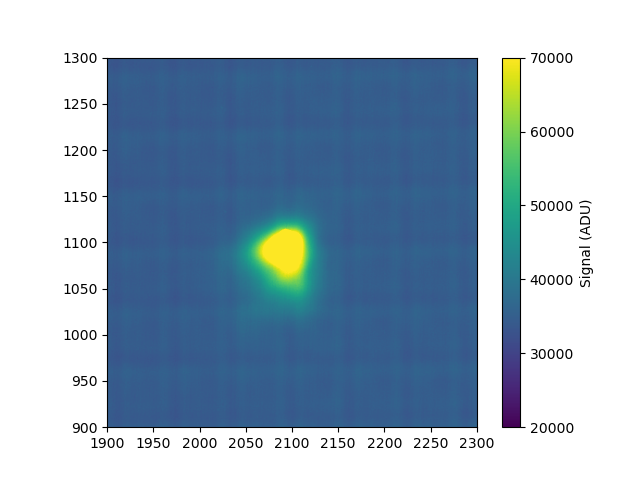
\includegraphics[width=0.48\textwidth]{figures/Spot_Spot_Ex.png}
\caption{(left) Example of a spot image zooming into a single detector. (right) Example of a spot image zooming further into a single spot. In both the images, there is a clear background structure caused by the projector.}
\label{fig:SpotProjector_Spots}
\end{figure}

\begin{figure}[htbp]
\centering
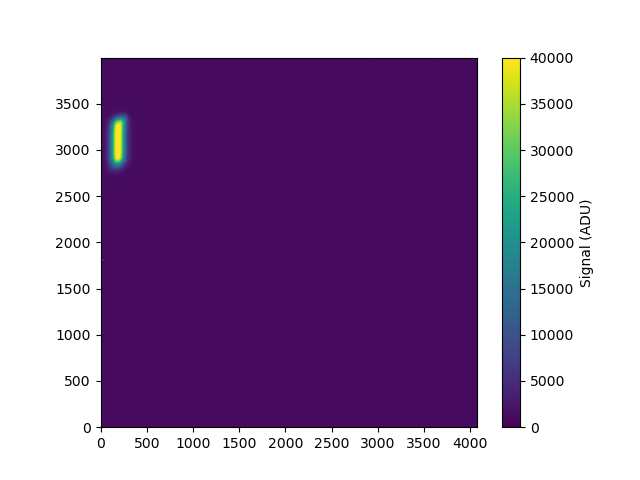
\includegraphics[width=0.32\textwidth]{figures/Rectange_Detector_Ex.png}
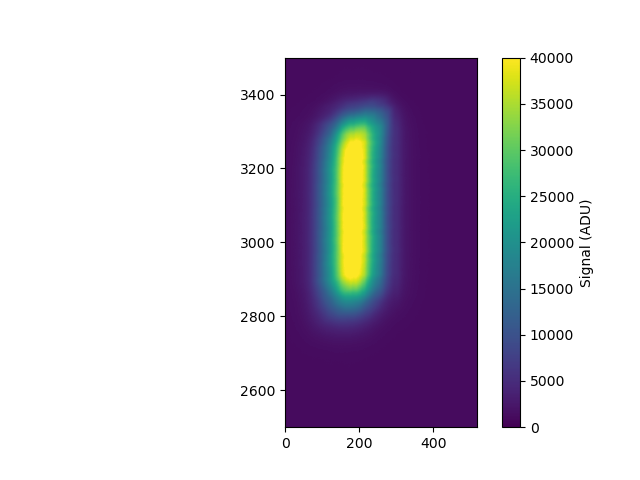
\includegraphics[width=0.32\textwidth]{figures/Rectange_Spot_Ex.png}
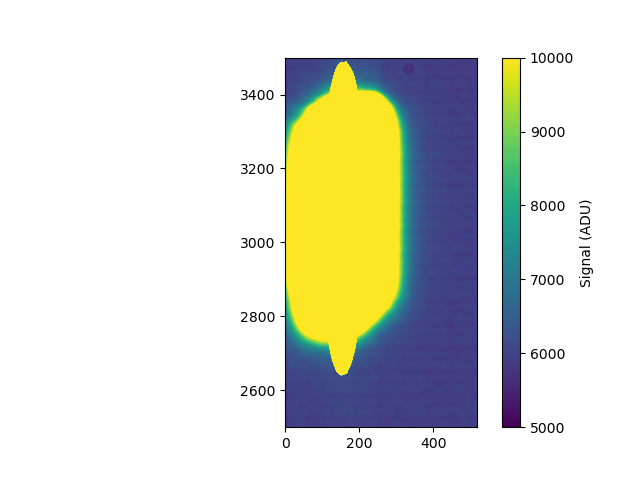
\includegraphics[width=0.32\textwidth]{figures/Rectange_Spot_Sat.png}
\caption{(left) Example of a spot image that utilized the rectangle shape, zoomed into a single detector (left), zoomed into the spot (middle) and zoomed into the spot with a saturated image to highlight the background pattern caused by the projector (right).}
\label{fig:SpotProjector_Rect}
\end{figure}

This section describes the spots and rectangle patterns used for tests with the 4K
projector.

\begin{itemize}
\tightlist
\item  Projector background
\item  Spots on many amps
\item  Spots on one amp
\item  Optical setup
\end{itemize}

\subsection{Dark current and light
leaks}\label{dark-current-and-light-leaks}

%This section describes dark current and light leaks in Run 7 testing.

\subsubsection{Light leak mitigation with shrouding the camera
body}\label{light-leak-mitigation-with-shrouding-the-camera-body}

One of the first tests we attempted with LSST Camera was measuring dark
current and sources of light leaks in the camera body. Before beginning we covered gaps between the L1 cover and the gaskets with tape, in accessible locations . Figure \ref{fig:L1_Gaps} shows the gaps that we could see between L1 and its cover. The inaccessible locations were later covered with shroud.

\begin{figure}[htbp]
\centering
\includegraphics[width=0.48\textwidth]{figures/L1_Gap1.png}
\includegraphics[width=0.48\textwidth]{figures/L1_Gap2.png}
% 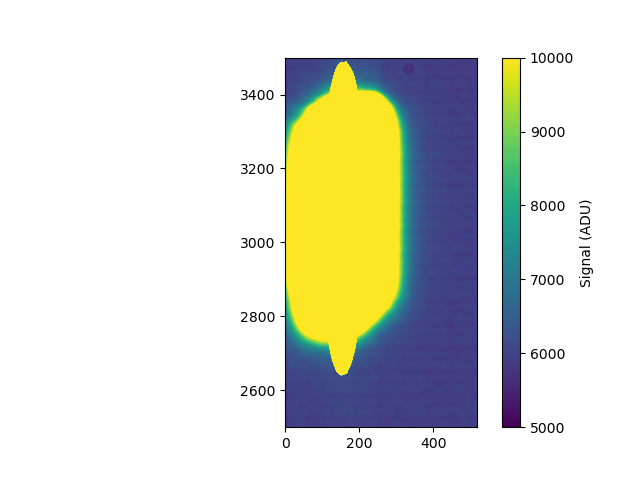
\includegraphics[width=0.32\textwidth]{figures/Rectange_Spot_Sat.png}
\caption{Example photos of the L1 cover gaps. These were covered by tape where we could safely apply it and by the black shroud.}
\label{fig:L1_Gaps}
\end{figure}

Once these were sealed, we took some initial measurements and then
started to cover the LSST Camera body with a Thorlabs blackout fabric shroud (BK5). Figure~\ref{fig:LSSTCam_config} shows the final configuration of the shroud covering the
camera.
We also found light leaks where the light cone attached to L1 was housed, and from the Utility Trunk, which were covered with shroud. Table~\ref{tab:leak_chasing} includes the observations, the corresponding measured dark currents, and comments on what changed during the chasing of the leaks.

{\small
\begin{longtable}[ht]{|l|c|l|l|l|}
\caption{Summary of the 15\,s dark exposures, the different conditions, and the resulting dark current.
Exposure ID is preceded by ``MC\_C202409".  The shroud was in place for each of these measurements.  (``Initial Covering" was just the CCOB cone and around the L1 cover.) \label{tab:leak_chasing}} \\
\hline
\textbf{Exposure} & \textbf{Dark Current} (ADU/s) & \textbf{Room Lights} &\textbf{Shutter} & \textbf{Comments} \\

\hline
\endfirsthead
\hline
%\textbf{Exposure ID} & \textbf{Dark Current (e$^-$/s)} & \textbf{Room Lights} & \textbf{Shutter} & \textbf{Comments} \\
\hline
\endhead
\hline
\endfoot
\hline
09\_000012 & 0.16 & Off & Closed & \\
09\_000018 & 0.16 & On & Closed & \\
09\_000038 & 2.94 & On & Open & Initial Covering  \\
09\_000054 & 1.34 & On & Open &  + Blanket over the FCS \\
09\_000072 & 0.41 & On & Open &  + Blanket over AND under the FCS \\
09\_000078 & 0.18 & Off & Open & + Blanket over AND under the FCS \\
10\_000031 & 0.03 & On & Open &  + Blanket over AND under the FCS + UT \\

\end{longtable}
}


\subsubsection{Filter Exchange System Autochanger light leak
masking}\label{successful-autochanger-light-leaks-masking}

A dedicated light leak study of the Filter Exchange System (FES) Autochanger (AC) was performed during Run 6 at SLAC
in summer 2023 and a localized faint light source of up to
\textasciitilde{}0.04 e$^-$/s/pix was found to be associated with the 24\,V Clean of
the AC.

In the AC this voltage is used to power some probes and all
controllers. In February 2024, as AC-1 was extracted from LSST Camera for
global maintenance, a direct investigation to localize the light
source was performed unsuccessfully. A light source in the AC
was not expected, as in the AC all controllers' LEDs have
been removed, and most electronics are in ``black boxes". Still, two small
probes, which had LEDs that could not be removed, were initially masked
by a black epoxy. As we had doubts about the quality of this masking at
IR wavelengths, we applied extra masking (aluminum black tape) on them during
the Feb 2024 maintenance (on AC 1 and 2).

At the start of Run 7 a new study of the light leak based on 900\,s
dark exposures with the shutter open and the empty frame filter in
place, showed that the AC light leaks were still present (see left-hand image of Fig.~\ref{fig:ac-light-leak}). Following this finding, a full review of all the AC hardware powered
by the 24 V dirty was performed, and a candidate was found: the encoders
of the five main motors of the AC had only partial documentation from the
vendor that did not mention the presence of LEDs. After interaction with the
vendor, the encoders were understood to contain \textasciitilde700\,nm LEDs. The hypothesis of \textasciitilde700\,nm LED sources has been
found compatible with the observation as no AC light leaks were detected
using various filters (g, r, and y ; all opaque at 700 nm ) in LSST Camera at the start of Run 7 (g, r, and y
filters). A dedicated test in Paris using an AC spare encoder and a
precision photometric set-up allowed identification of the leak in the masking of
those LEDs in the vendor packaging (see Figure \ref{fig:CoderLight}). A complementary masking method based
on a 3D printed part + tape + cable tie was qualified in Paris.  It was
found to mask the light leak and to be safe (all parts correctly secured, see Figure \ref{fig:CoderLight})).

In November 2024, we masked all the lights in the back of the Level 3 white
room (not the part containing LSST Camera) to set up a high-quality dark room
allowing a direct observation with a CMOS camera of the light leak on
the AC2 motor encoders. The level of darkness reached allowed us to
validate the quality of the light masking of the AC encoders. Notice that the
FES-prototype in Paris does not have encoders on the Online
Clamps, so we had to tune/qualify the masking of those encoders directly on the AC 2 at the summit.

For both AC 1 and 2, the encoders of the five motors with the vendor issue on
their LED masking have been successfully enveloped in a light-tight
mask (see Figure \ref{fig:CoderLight}).

We note that the AC was turned off starting on 27 September 2024 at 21:15 UTC in the
first part of Run 7. For the second part of Run 7 (i.e., after
mid-November) the AC was back on: as the AC 1 was back in LSST Camera with
the new light masks in place on the motor encorders, we were able to take a new series of
900\,s darks with the AC turned on and off, confirming that the light leak
associated with the FES was eliminated (see right-hand image of Fig.~\ref{fig:ac-light-leak}).
\begin{figure}[ht]
\centering
\begin{subfigure}{0.32\textwidth}
  \centering
  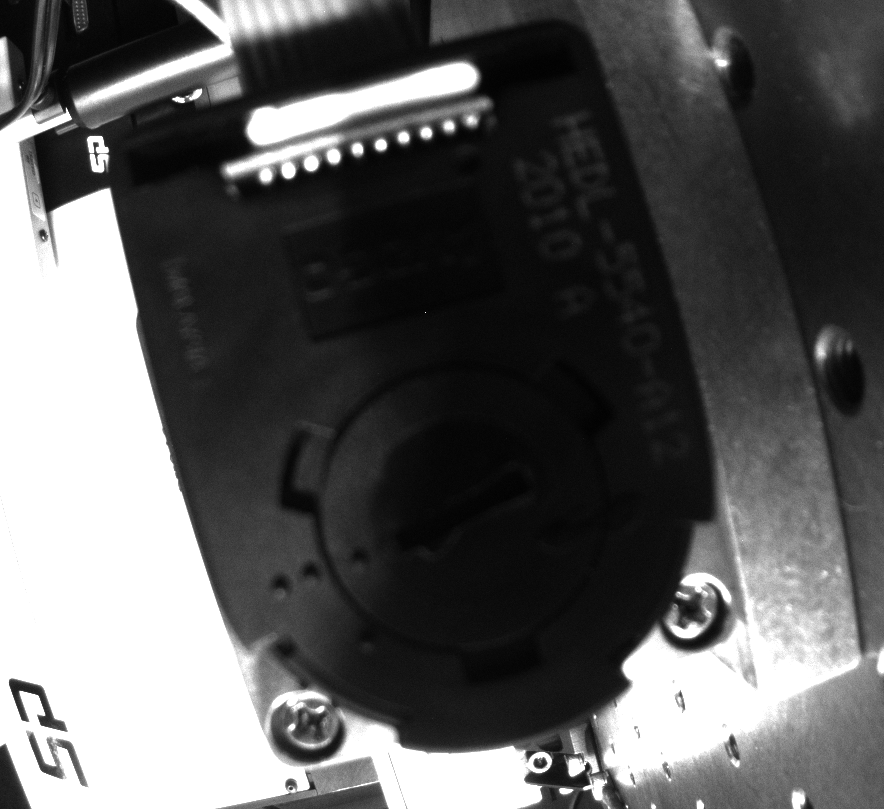
\includegraphics[width=1.0\textwidth]{figures/Codershape.png}
\end{subfigure}%
\begin{subfigure}{0.32\textwidth}
  \centering
  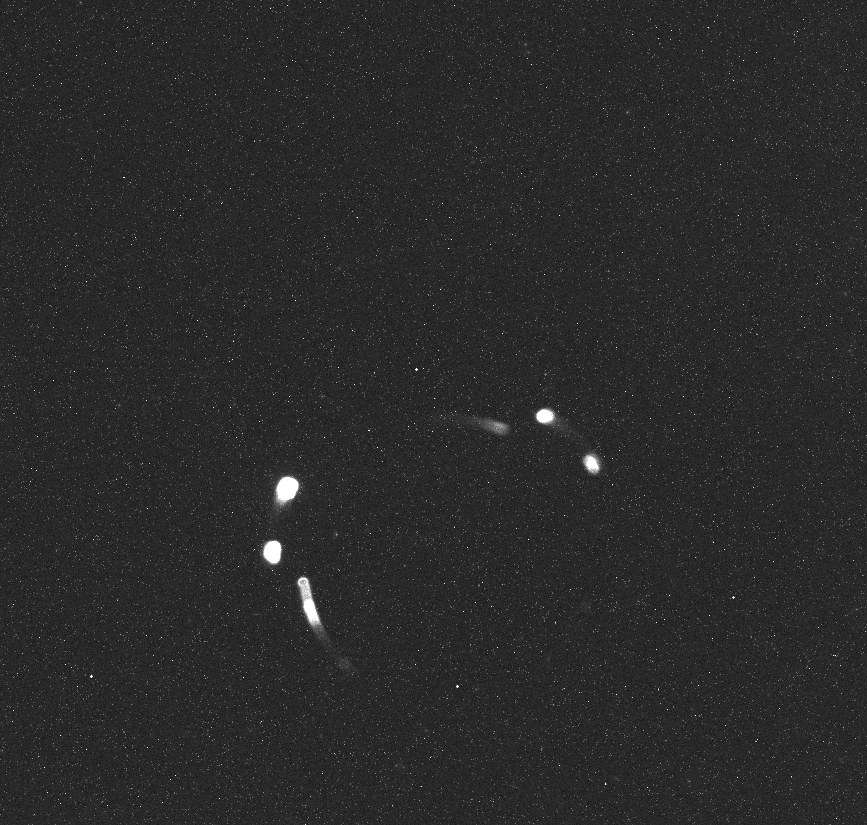
\includegraphics[width=1\textwidth]{figures/Coderligth.png}
\end{subfigure}
\begin{subfigure}{0.32\textwidth}
  \centering
  \includegraphics[width=1\textwidth]{figures/X-OnlineCoder.png}
\end{subfigure}
\caption{On the left a picture of one AC coder . In the center a 60\,s exposure , with the same coder On , light in the room off : light leak is obvious , mainly associated to holes on the top of the coder cover . On the left , the X- Online coder after masking .}
\label{fig:CoderLight}
\end{figure}

\begin{figure}[ht]
\begin{centering}
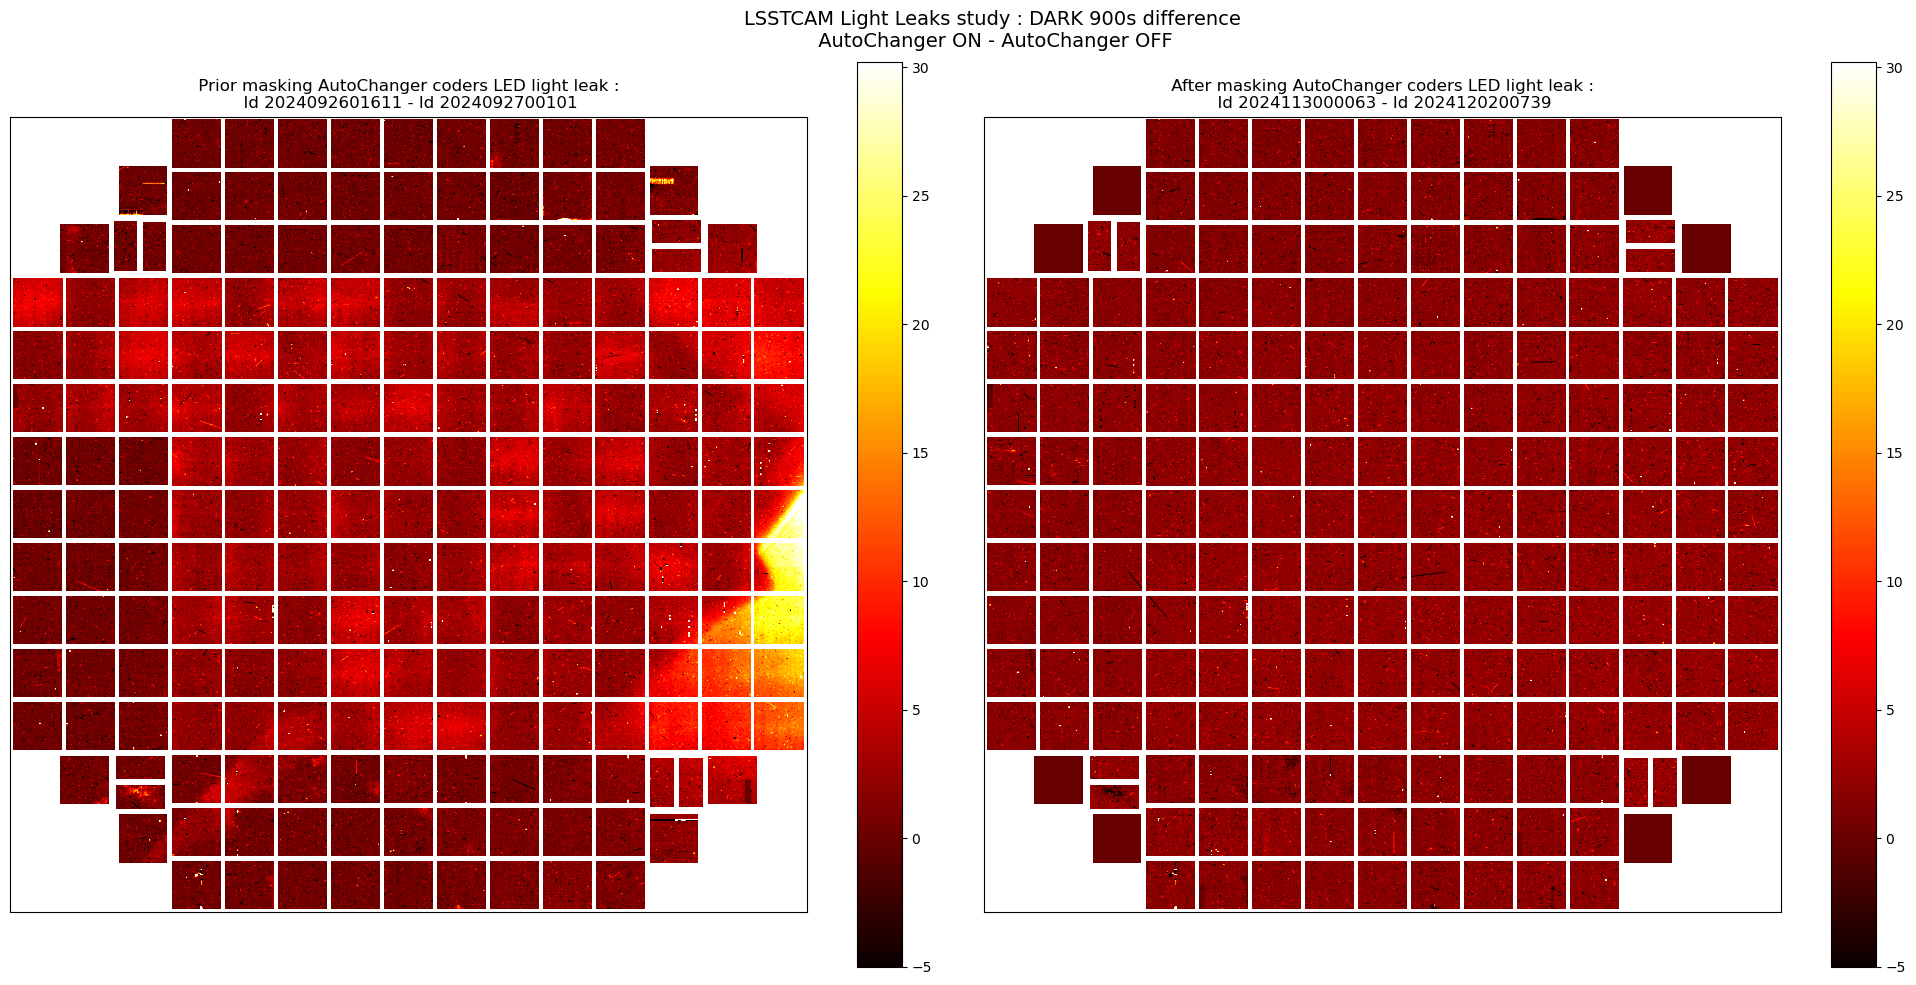
\includegraphics[width=0.8\textwidth]{figures/AC_LightLeak_study.png}
\caption{ (left) The original impact of the AC light leak on a 900\,s dark difference image (AC on minus AC off), we observe in particular a ``bright triangle" on the right of this focal plane image. We also note the presence of the persistence of \textasciitilde 10 ADU for a few sensors, the same e2v sensors than the one visible in the left figure \ref{fig:persistence-reduction}. We did not collect the exactly same condition image, a dark without the AC leak mitigation with the persistence mitigation voltages (see Sect. \ref{persistence-optimization-1}). (right) The result after masking the LEDs of the motor encoders in the AC.  No light associated with the FES is present in 900\,s dark difference image.  \label{fig:ac-light-leak}}
\end{centering}
\end{figure}

\subsection{Shutter condition impact on
darks}\label{shutter-condition-impact-on-darks}

Two runs, E1075 and E1076, were dedicated to determining the effect of the shutter on darks by keeping the shutter closed and open respectively. Figure \ref{fig:shutter-darkcurrent} shows example images of the focal plane from both of these runs. 
Figure \ref{fig:DarkCurrent_ShutterOpenvClosed} shows the difference between the shutter open and closed and how this condition affects the dark current.
No easily visible difference can be seen between the two images. This is most likely due to the shrouding of the camera (see Section \ref{light-leak-mitigation-with-shrouding-the-camera-body}) as well as the pinhole filter being in place for these runs.

\begin{figure}[ht]
\begin{centering}
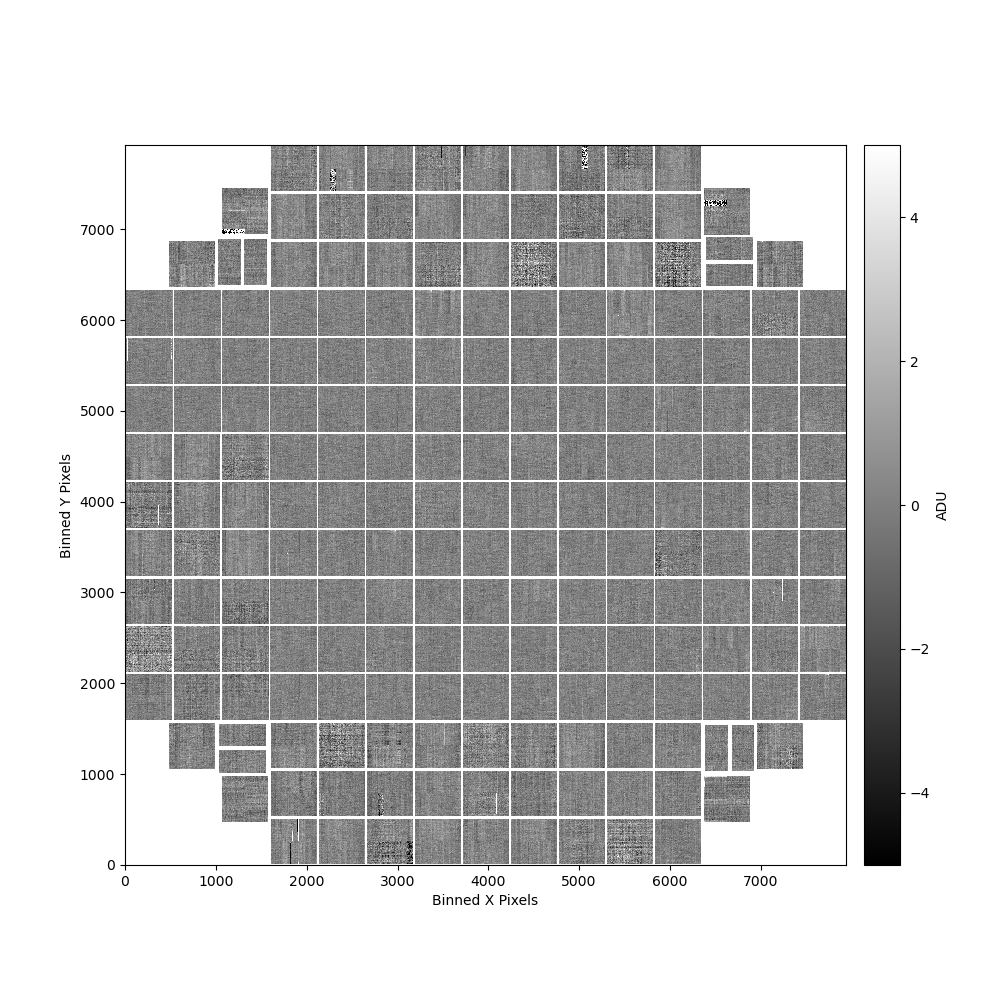
\includegraphics[width=0.48\textwidth]{figures/E1075_ShutterClosed.png}
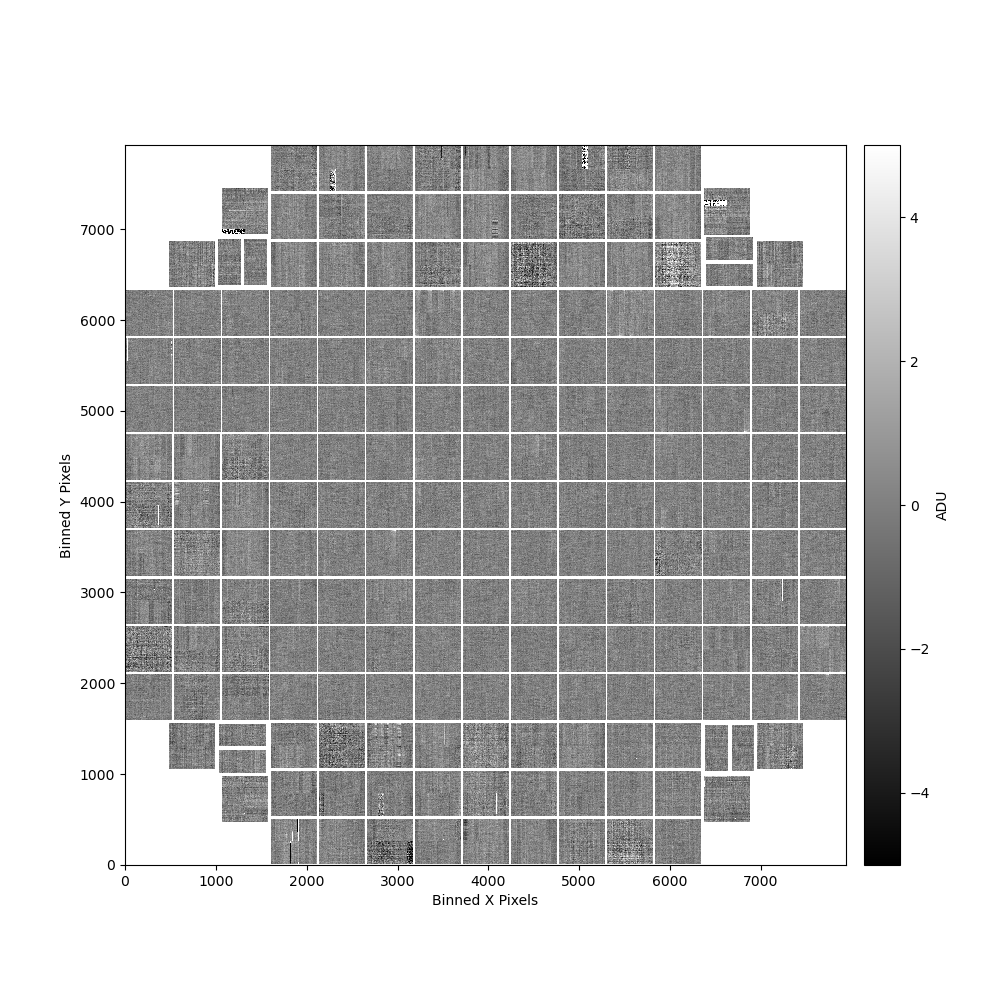
\includegraphics[width=0.48\textwidth]{figures/E1076_ShutterOpen.png}
\caption{ (left) An example image of run E1075 (shutter closed). (right) An example image of run E1076 (shutter open). If there was a light leak, we would expect to see the 21 spots of the pinhole filter. However, there is no noticeable difference between the images, confirming that our shrouding described in Section \ref{light-leak-mitigation-with-shrouding-the-camera-body} is good and that the shutter being open and closed does not affect the dark current. \label{fig:shutter-darkcurrent}}
\end{centering}
\end{figure}

\begin{figure}[ht]
    \centering
    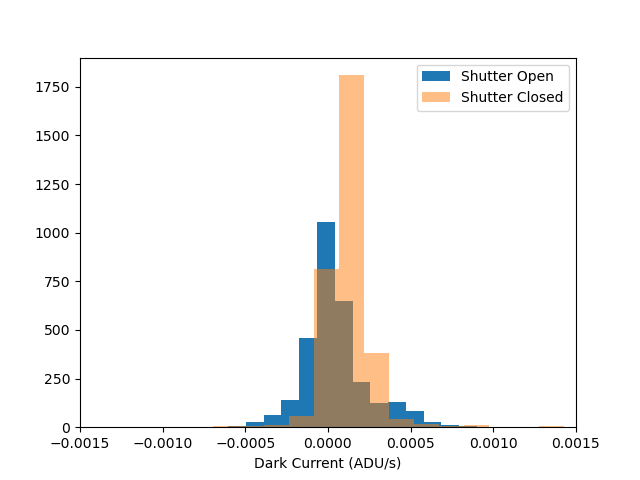
\includegraphics[width=0.5\linewidth]{figures/DarkCurrent_ShutterOpenvClosed.png}
    \caption{Histogram comparison between the dark current between the shutter being open versus closed.}
    \label{fig:DarkCurrent_ShutterOpenvClosed}
\end{figure}

\subsection{Impact of filters on dark images}\label{filter-condition-impact-on-darks}

To investigate how the filter affects the dark measurement, we took 900\,s darks with the available filters in the filter wheel: E1114 (empty filter), E1115 ($g$), E1116 ($y$), and E1117 ($r$). The heat maps of the dark currents from {\tt eo\_pipe} can be found in Figure~\ref{fig:filter-darkcurrent}. The major effect of including the filters was reducing the glow the AC (see Figure \ref{fig:ac-light-leak}). The global average of the median amplifier dark currents decrease from $26 \times 10^{-3}$ e-/s with the empty filter to $3.5 \times 10^{-3}$ e-/s for $r$, $1.1 \times 10^{-3}$ e-/s for $y$, and $0.63 \times 10^{-3}$ e-/s for $g$. The discrepancy between the filters could arise if the AC light shines more brightly in the redder wavelengths and even the IR. Unfortunately, we were not able to obtain data with the other three filters to confirm this.

\begin{figure}[ht]
\begin{centering}
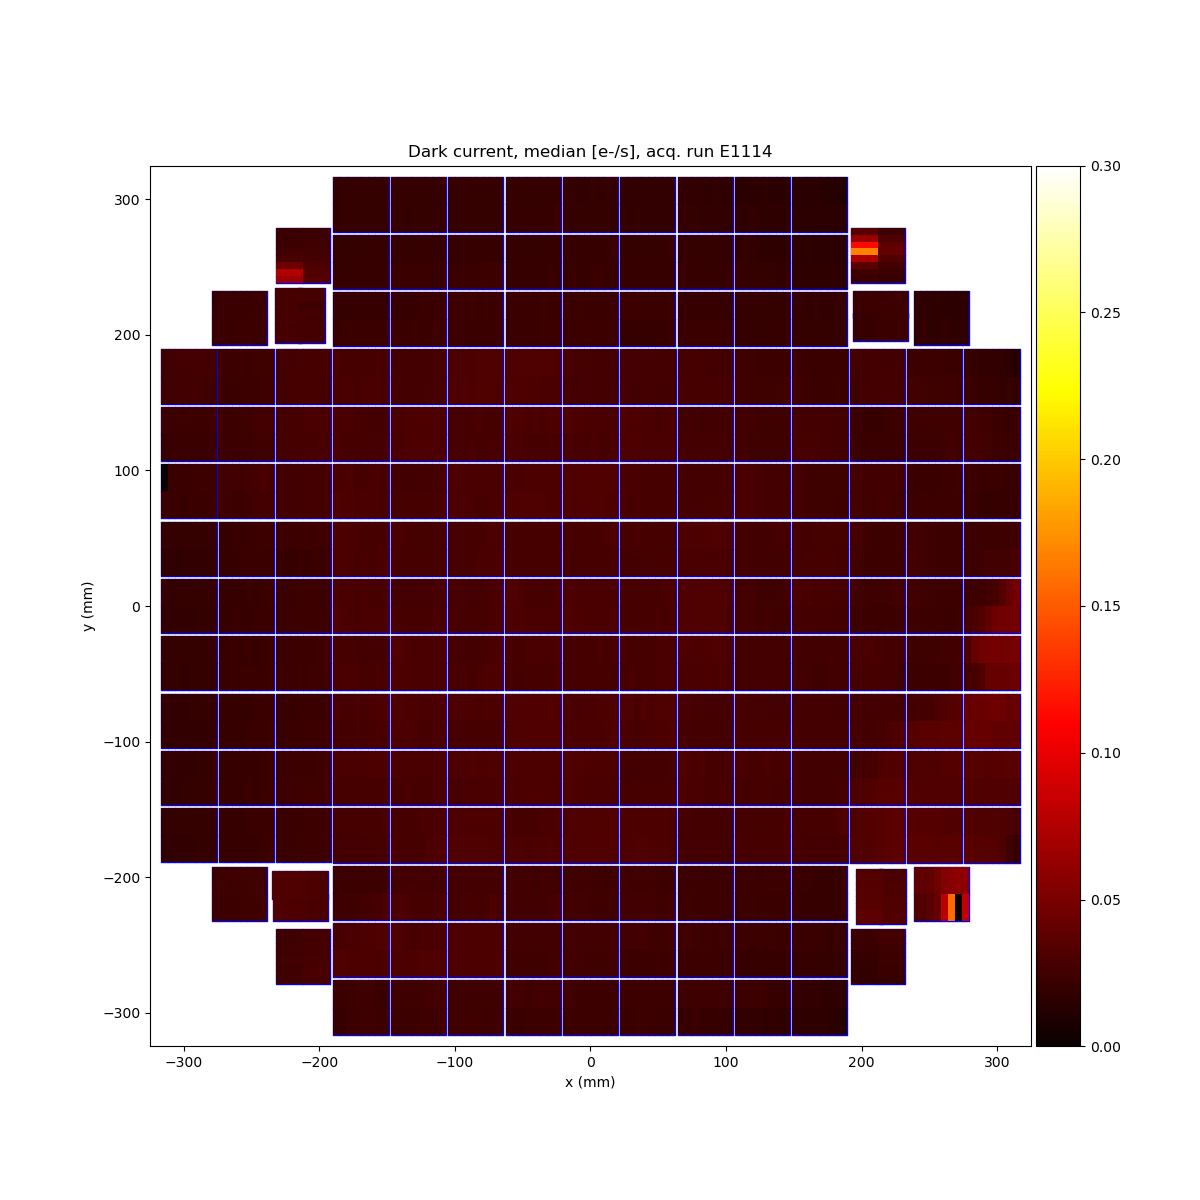
\includegraphics[width=0.48\textwidth]{figures/E1114_Empty_DarkCurrent.png}
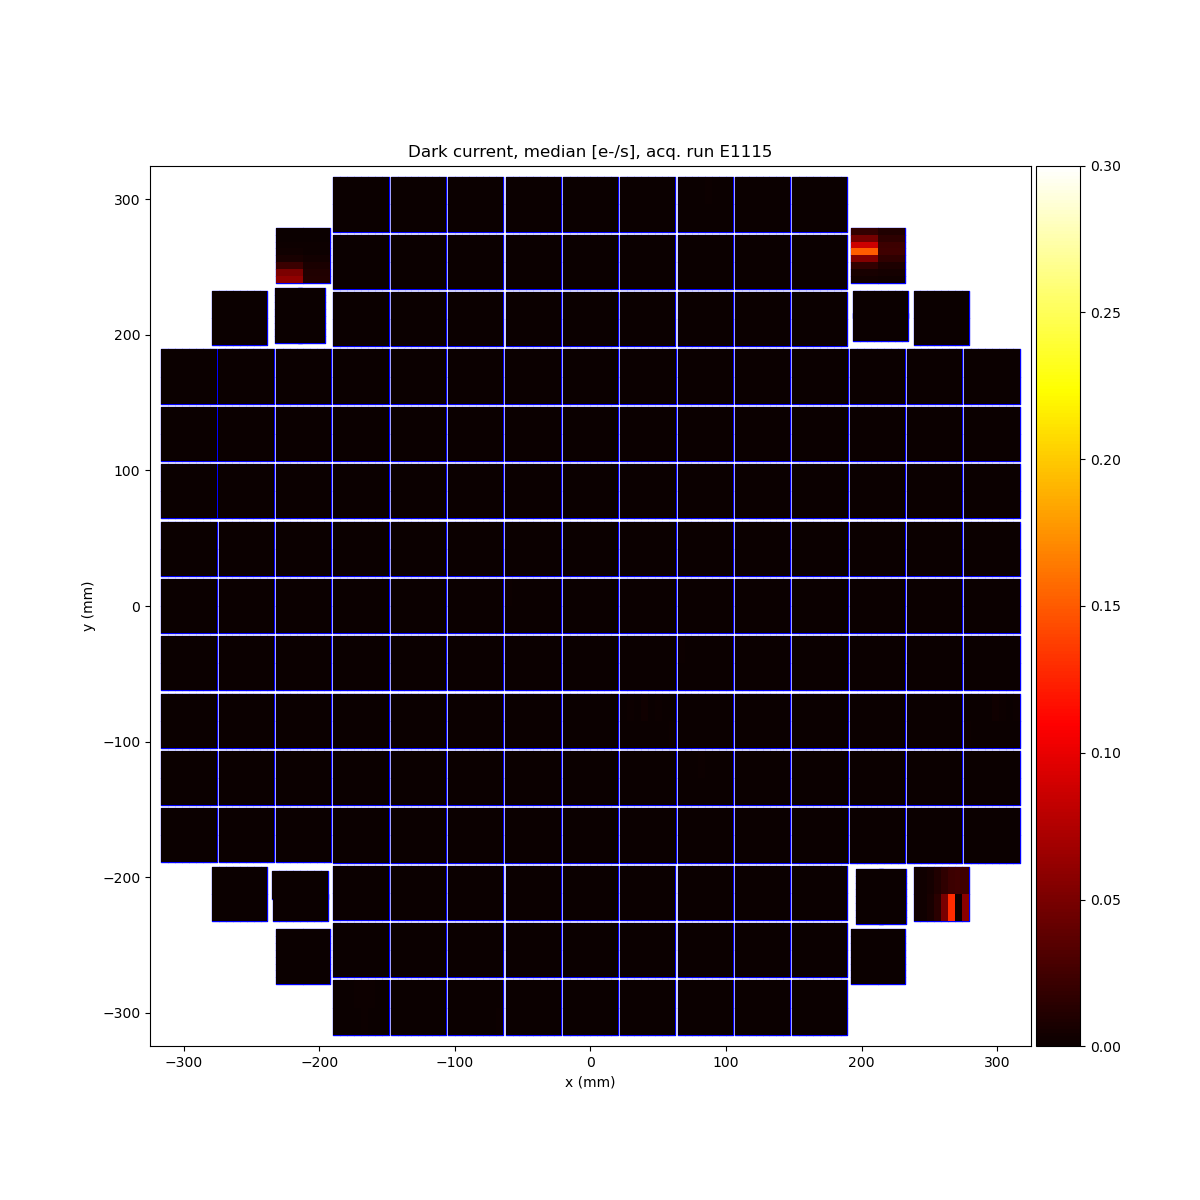
\includegraphics[width=0.48\textwidth]{figures/E1115_g_DarkCurrent.png} \\
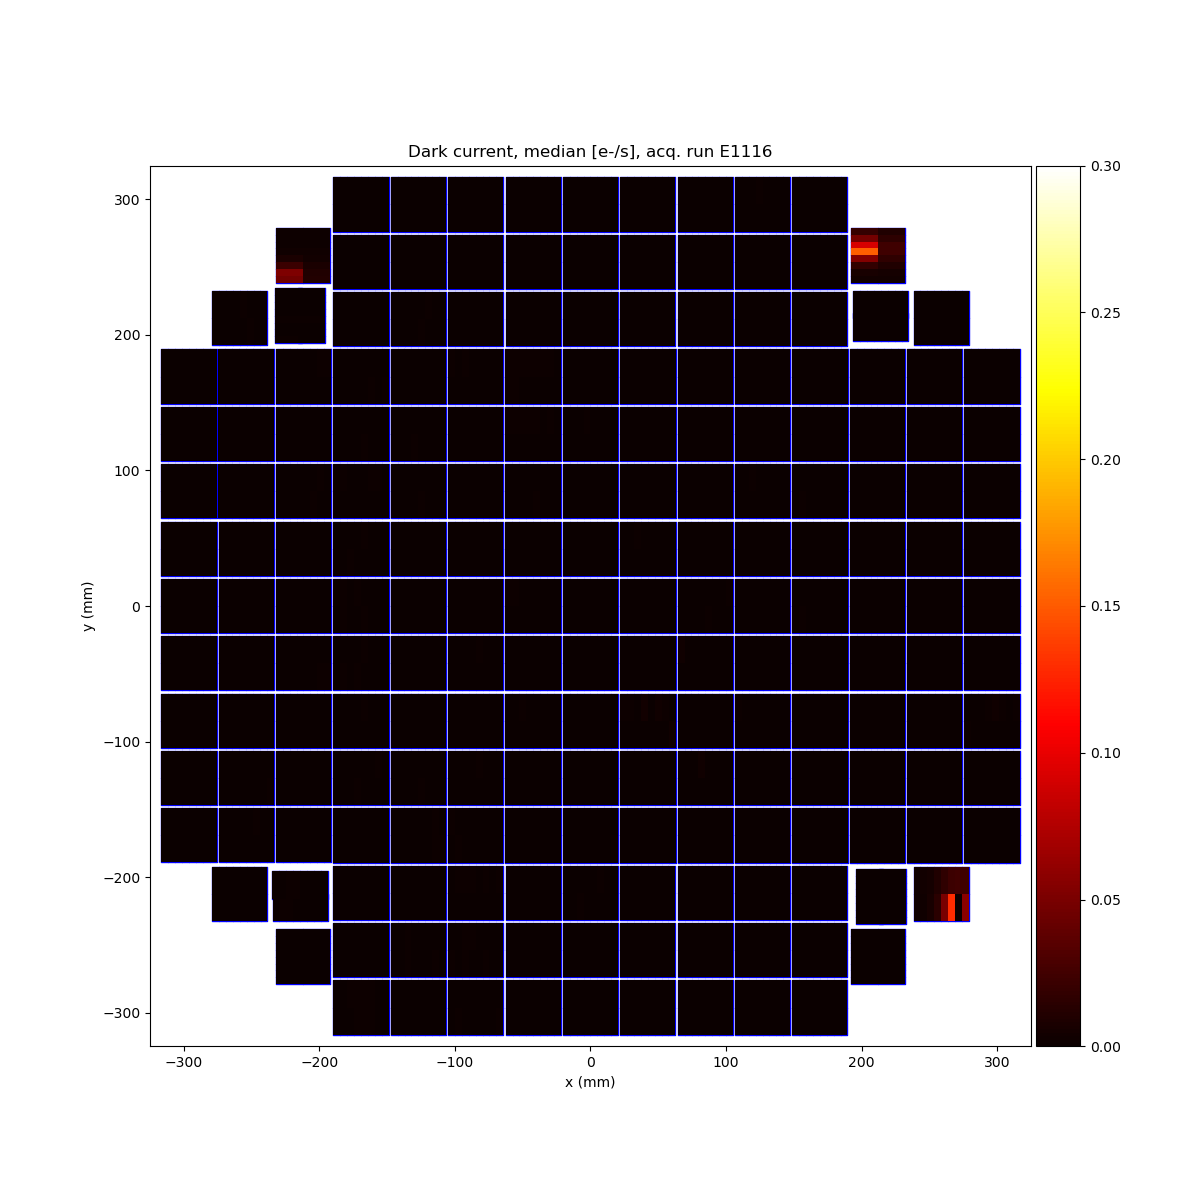
\includegraphics[width=0.48\textwidth]{figures/E1116_y_DarkCurrent.png}
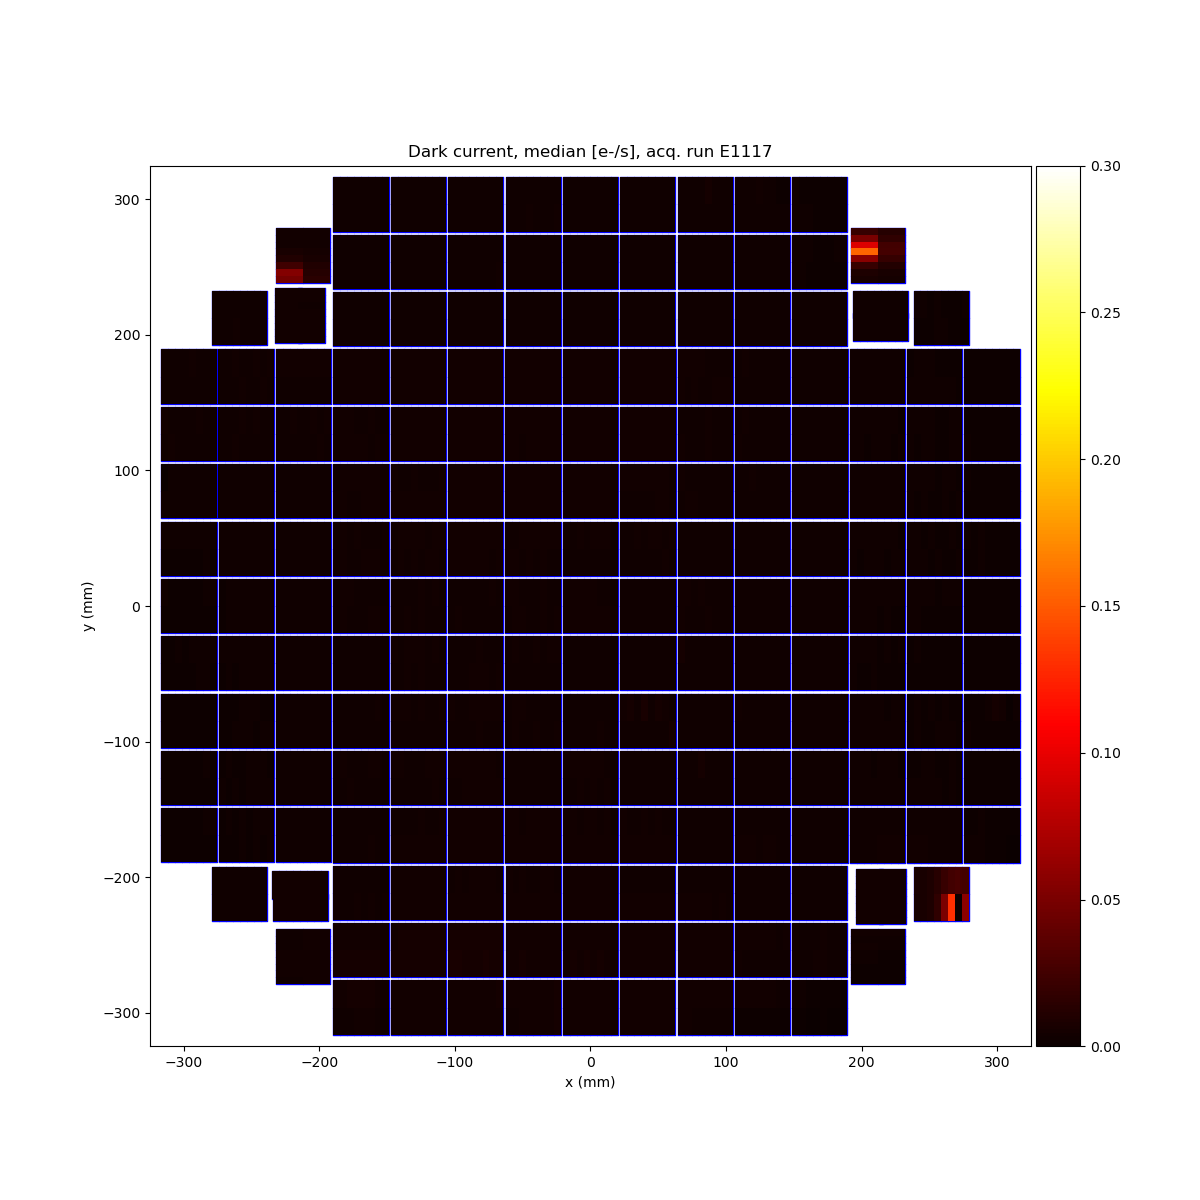
\includegraphics[width=0.48\textwidth]{figures/E1117_r_DarkCurrent.png}
\caption{ The heat map of the dark current with the empty filter installed (E1114; top left), the $g$ filter installed (E1115; top right), the $y$ filter installed (E1116; bottom left), and the $r$ filter installed (E1117; bottom right)  \label{fig:filter-darkcurrent}}
\end{centering}
\end{figure}

%\subsubsection{Final measurements of dark current}\label{final-measurements-of-dark-current}
% we don't need this since it will be compared in the following sections.

\clearpage

\clearpage

\section{Reverification}\label{sec:reverification}

All EO camera test data is processed through the
\underline{\href{https://github.com/lsst/cp_pipe/tree/main}{calibration products}} and
\underline{\href{https://github.com/lsst-camera-dh/eo_pipe/tree/main}{electro-optical}}
pipelines to extract key metrics from the data run. The key LSST Camera
metrics from Run 7, and their comparison to previous runs are discussed
below.




Among the motivations for these measurements, the primary concern is whether LSST Camera has
maintained its performance characteristics between Run 6 and Run 7, since LSST Camera was transported from SLAC to Cerro Pachon.
The testing condition is supposed to be identical; however as described in Section \ref{brighter-fatter-a00-coefficient}, two rafts have slightly different voltages between two runs.

\subsection{Background}\label{background}

Initial characterization studies performed on LSST Camera during Run 7 primarily used two
image acquisition sequences.

\begin{itemize}
\tightlist
\item
  B protocols: this acquisition sequence consists of the minimal set of
  camera acquisitions for EO testing, including

  \begin{itemize}
  \tightlist
  \item
    Bias images
  \item
    Dark images
  \item
    Flat pairs - flat illumination images (flats) taken at varying flux levels
  \item
    Stability flats - flats taken at constant flux levels
  \item
    Wavelength flats - flats taken with different LEDs
  \item
    A persistence dataset - a saturated flat, followed by several darks
  \end{itemize}
\item
  PTCs (photon transfer curves): this acquisition sequence consists of a
  sequence of flat pairs taken at different flux levels. The flat
  acquisition sequence samples different flux levels at a higher density
  than the B protocol flat sequence, enabling more precise estimates of
  flat pair metrics including pixel covariances (see Fig.~\ref{fig:PTC_BProtocol_Comparison}).
\end{itemize}

\begin{figure}[ht]
\begin{centering}
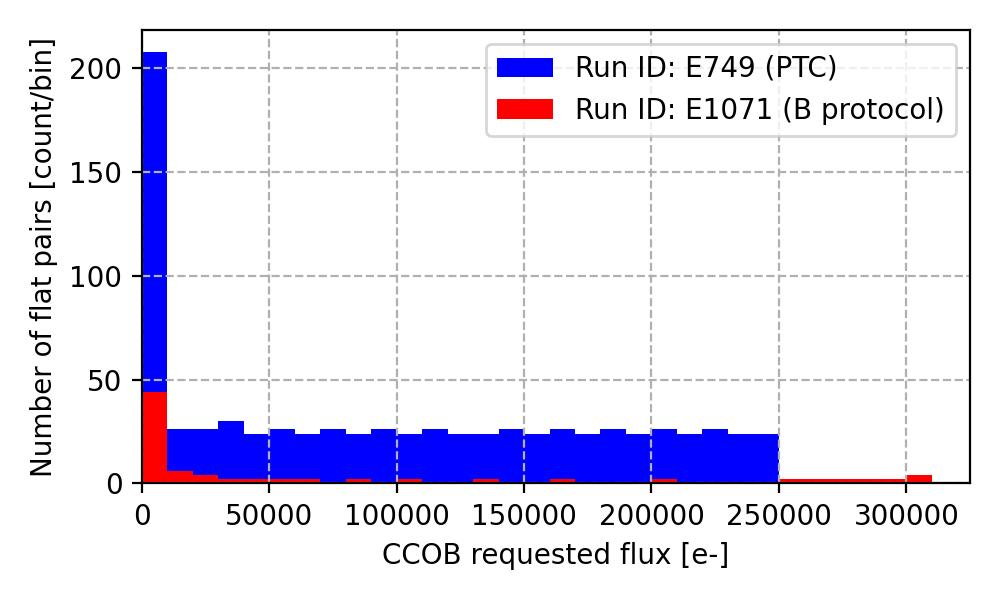
\includegraphics[width=0.7\textwidth]{figures/baselineCharacterization/PTC_BProtocol_Comparison.jpg}
	\caption{Flat-pair comparison between PTC and B protocol
\label{fig:PTC_BProtocol_Comparison}}
\end{centering}
\end{figure}

For comparisons between Cerro Pachon EO runs and the final SLAC IR2 equivalents, the following runs are used (see Table~\ref{runTable-b-ptc}).

\begin{table}[ht]
\centering
\caption{Reference runs for Run 6 and Run 7 comparisons} \label{runTable-b-ptc}
\begin{tabular}{lll}
\toprule
Run Type & Run 6 & Run 7 \\
\midrule
B Protocol & 13550 & E1071 \\
PTC        & 13591 & E749 \\
\bottomrule
\end{tabular}
\end{table}

The naming of the EO runs was established during initial LSST Camera
integration and testing. The final SLAC IR2 run from November 2023 was
named ``Run 6", while the data acquisitions from Cerro Pachon from September through December 2024 are considered ``Run 7". Additionally, individual EO acquisitions are tagged with a run identifier. This is commonly referred to as a Run ID. For all SLAC runs, the run identifier was a five digit numeric code, while the Cerro Pachon runs were ``E-numbers" that started with a capital E followed by a numeric code.


\subsection{Stability flat metrics}\label{stability-flat-metrics}

\subsubsection{Charge transfer
inefficiency}\label{charge-transfer-inefficiency}

CTI, or charge transfer inefficiency, measures the fraction of charge that fails to transfer from row to row during readout, and appears as trailing charge in the image area. Consequences of high CTI include loss of charge, distorted signals in the direction of parallel transfer, and reduced sensitivity in low light imaging. CTI measurements are made using the EPER method \citep{2021JATIS...7d8002S}, for which the ratio of the residual charge in the overscan pixels to the total signal charge in the imaging region is evaluated. In the context of LSST Camera, we measure CTI along both the serial and parallel directions.

\paragraph{Serial CTI}\label{serial-cti}

\begin{figure}[ht]
\begin{centering}
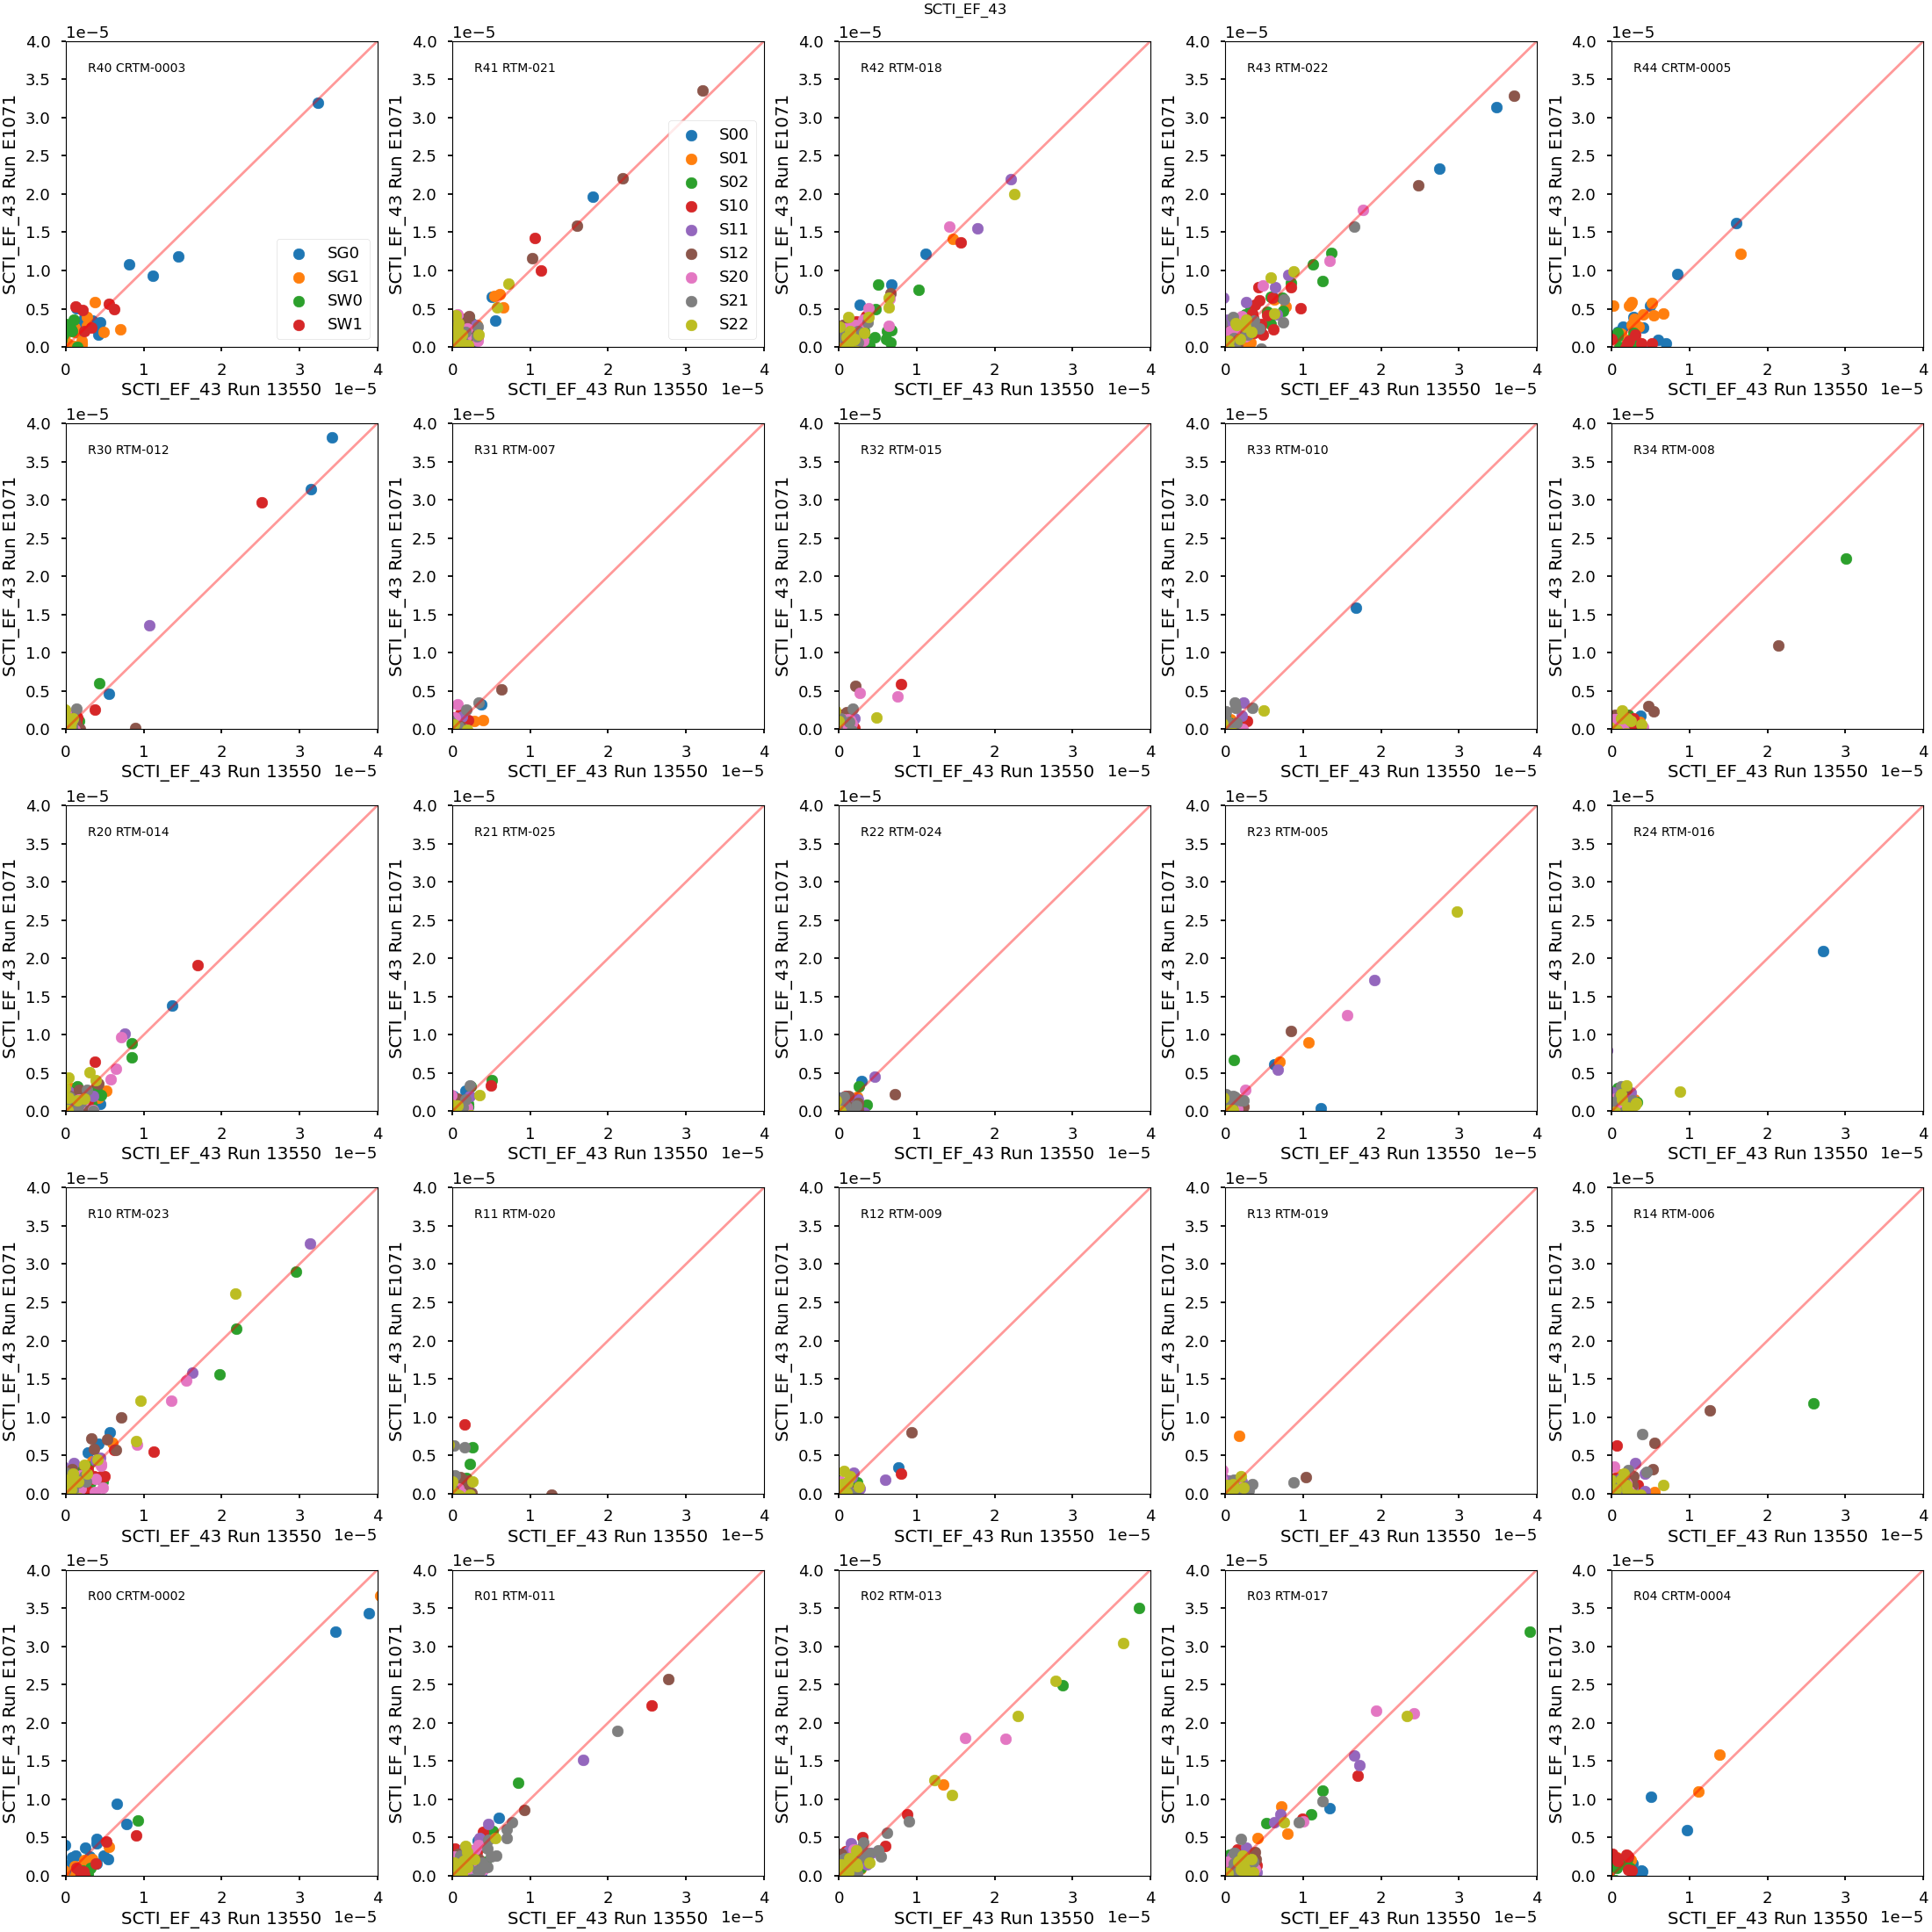
\includegraphics[width=0.7\textwidth]{figures/baselineCharacterization/13550_E1071_SCTI_EF_43_inset.png}
	\caption{Serial CTI amplifier measurements separated by raft for Run 7 (E1071) and Run 6 (13550)\label{fig:serial-cti}}
\end{centering}
\end{figure}

The CTI along the serial registers of the amplifier segments of the LSST Camera CCDs is consistent between Run 6 and
Run 7 (Fig.~\ref{fig:serial-cti}). Both sensor types show low CTI,
span a range  of \textasciitilde$2 \times 10^{-5}$ \% for e2v sensors, and
by \textasciitilde$4 \times 10^{-6}$  \% for ITL sensors (Fig.~\ref{fig:serial-cti-dist}). 

\begin{figure}[ht]
\begin{centering}
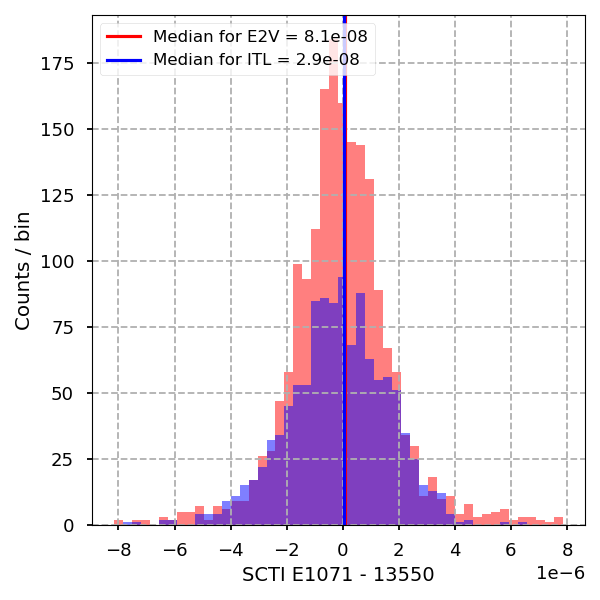
\includegraphics[width=0.7\textwidth]{figures/baselineCharacterization/SCTI_13550_E1071_diff.png}
\caption{Distributions of differences in serial charge transfer inefficiencies between Run 7 (E1071) and Run 6 (13550), grouped by CCD type.}
\label{fig:serial-cti-dist}
\end{centering}
\end{figure}

\clearpage
\paragraph{Parallel CTI}\label{parallel-cti}

The CTI along the parallel direction is consistent between Run 6 and
Run 7 (Fig.~\ref{fig:parallel-cti}). Both sensor types are found to have extremely low CTI on the order of $10^{-5}$ \%,
and span a range of \textasciitilde$1 \times 10^{-5}$ \% for e2v sensors, and
by \textasciitilde$7 \times 10^{-4}$ \% for ITL sensors (Fig.~\ref{fig:parallel-cti-dist}). Both of these measurements pass the CTI requirements (see table \ref{tab:initRever:Table}).

\begin{figure}[ht]
\begin{centering}
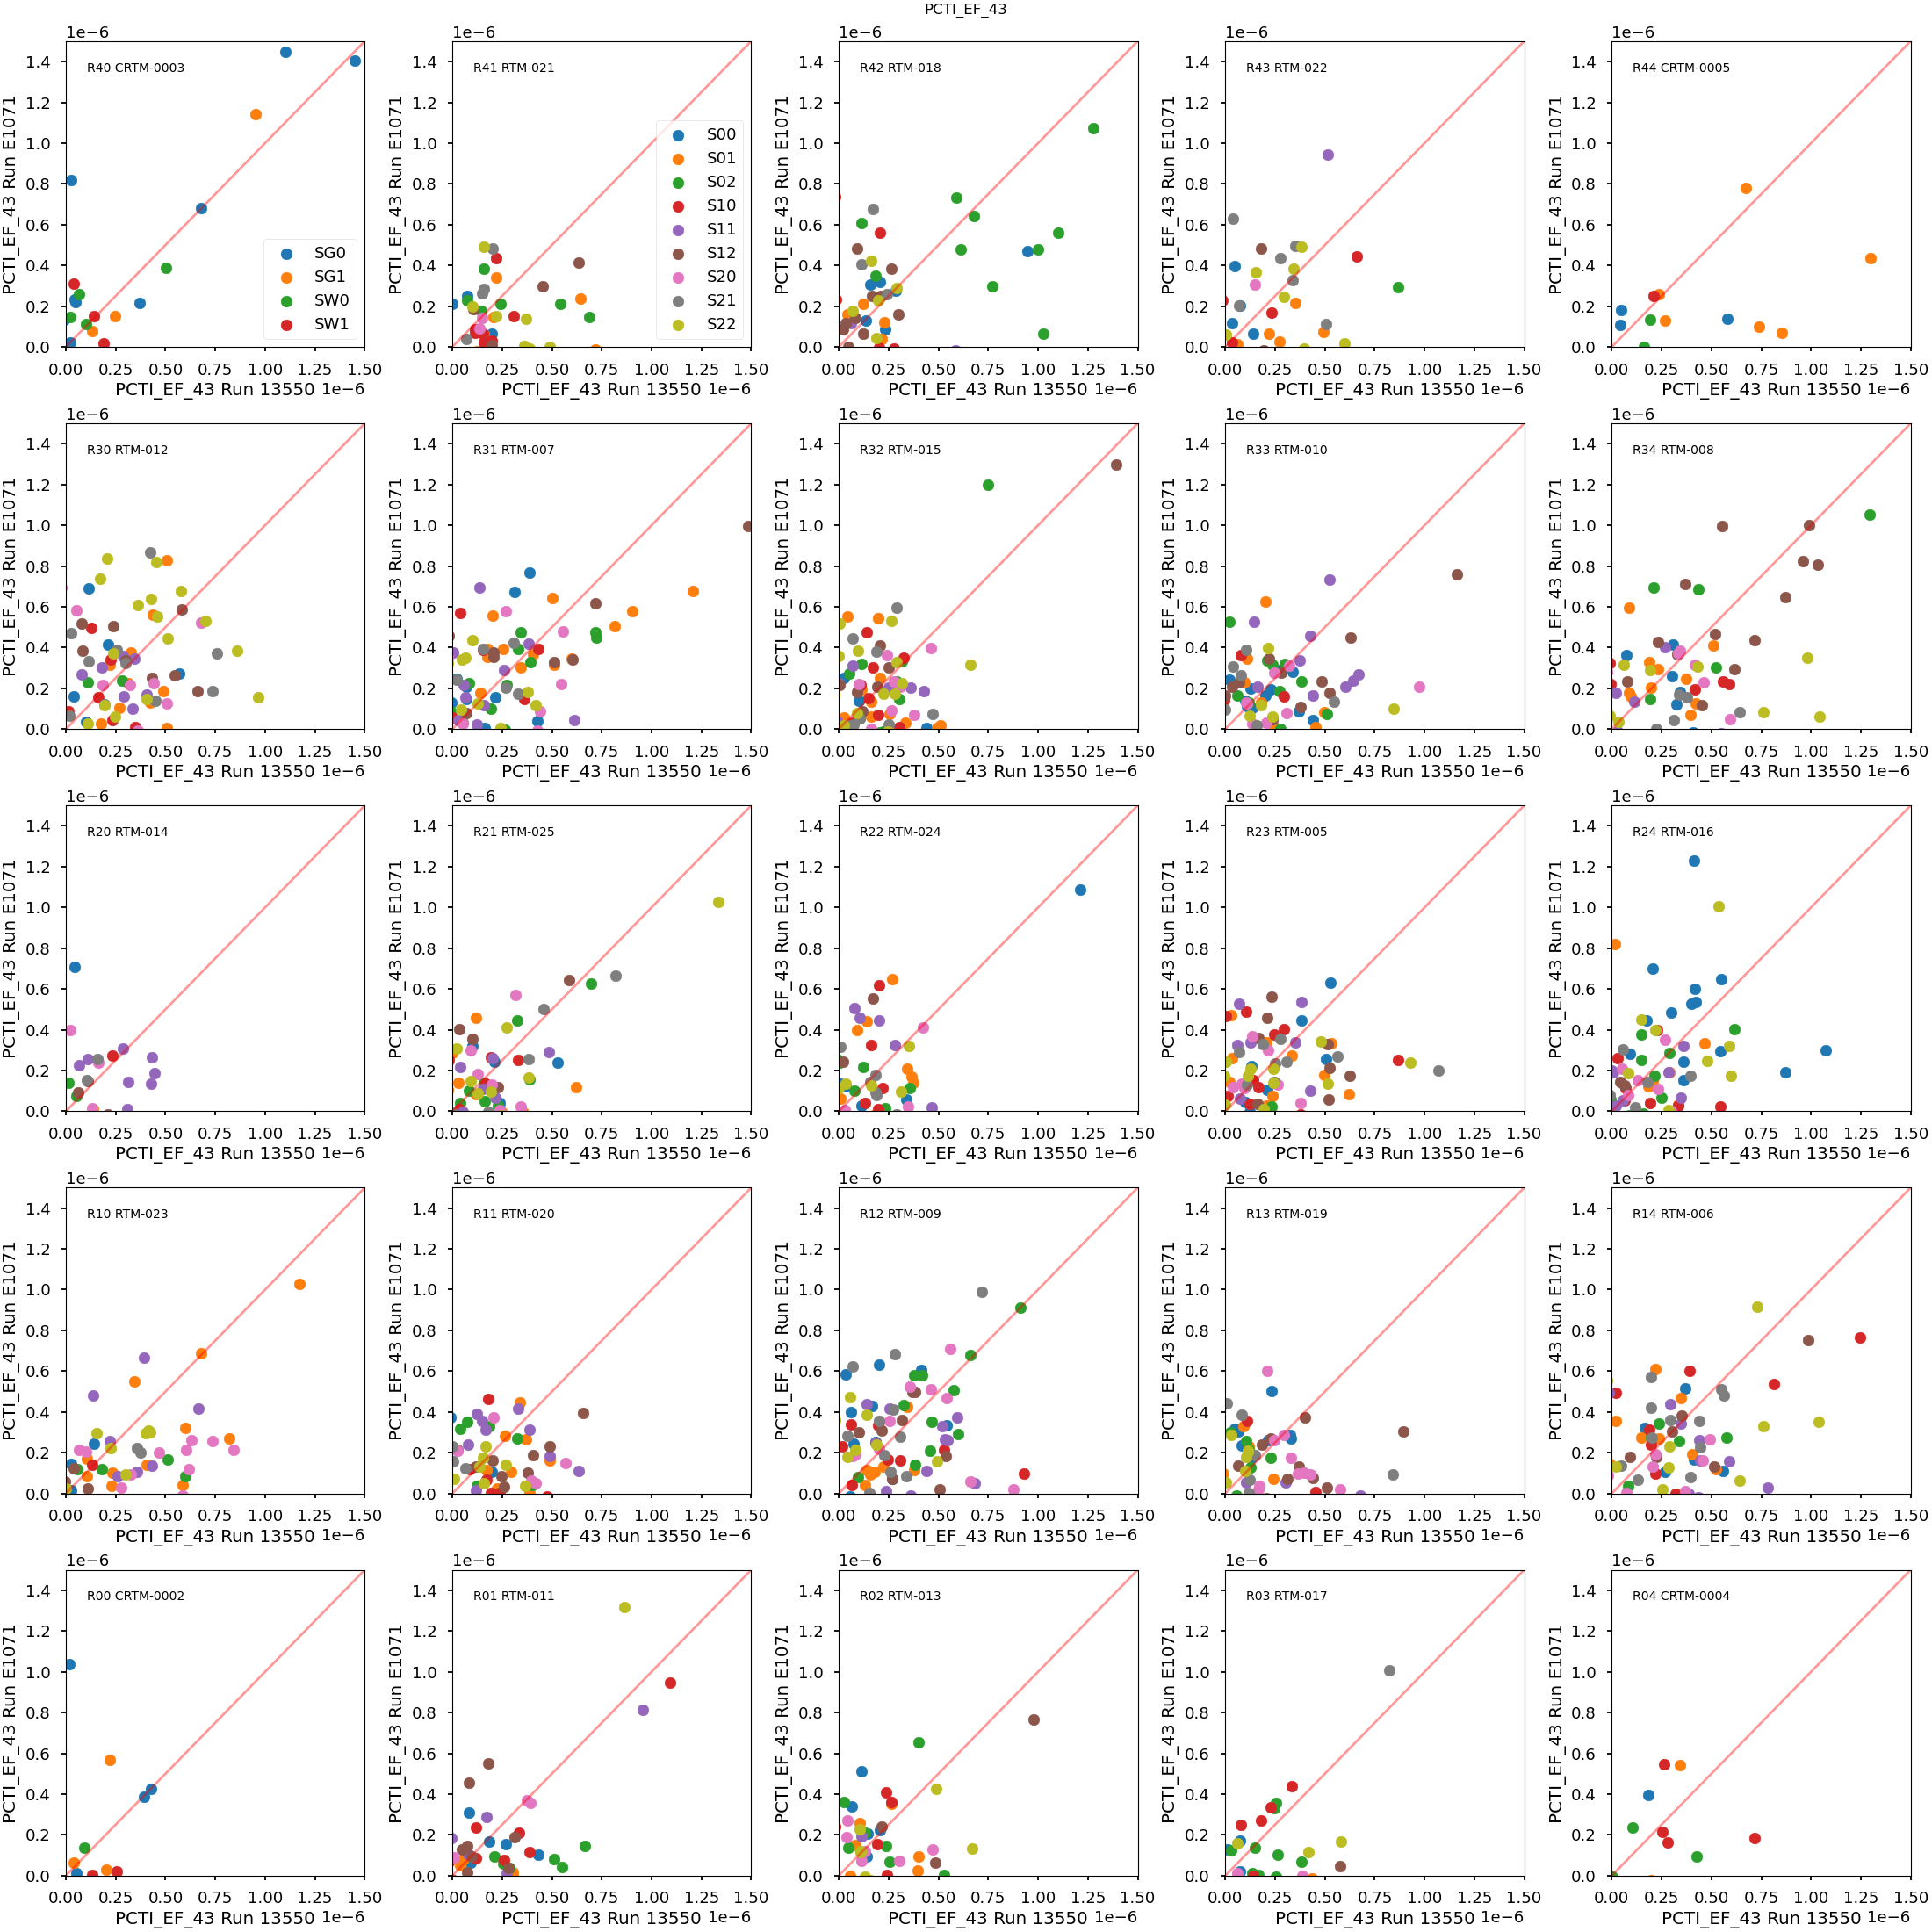
\includegraphics[width=0.7\textwidth]{figures/baselineCharacterization/13550_E1071_PCTI_EF_43_inset.png}
\caption{Parallel CTI comparison by raft for Run 7 (E1017) and Run 6 (13550).}
\label{fig:parallel-cti}
\end{centering}
\end{figure}

\begin{figure}[ht]
\begin{centering}
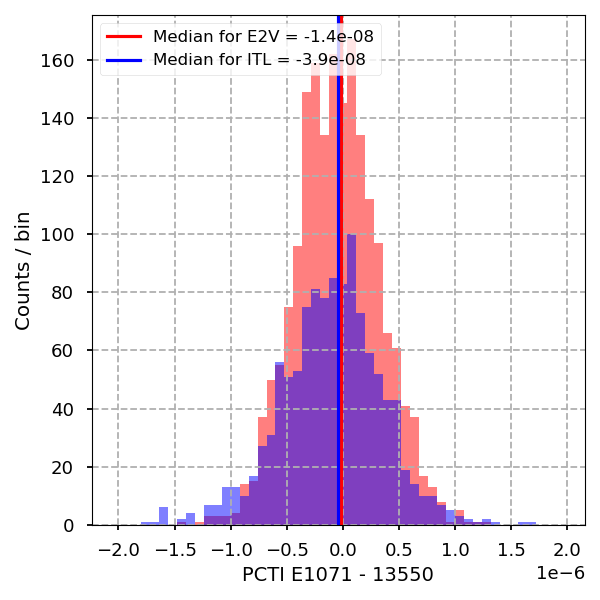
\includegraphics[width=0.7\textwidth]{figures/baselineCharacterization/PCTI_13550_E1071_diff.png}
\caption{Distributions of differences in parallel charge transfer inefficiencies between Run 7 (E1071) and Run 6 (13550), grouped by CCD type.}
\label{fig:parallel-cti-dist}
\end{centering}
\end{figure}

\clearpage
\subsection{Dark metrics}\label{dark-metrics}

\subsubsection{Dark current}\label{dark-current}

Dark current is the small amount of electrical charge generated in the
absence of light due to thermal activity within the semiconductor
material of a CCD. This effect occurs when electron/hole pairs are thermally released
into the conduction band in the CCD, mimicking the signal that light would
produce. Dark current increases with temperature, so cooling the CCD is
a common method to reduce it in sensitive imaging applications. Dark
current introduces noise into an image, particularly in low-sky background conditions in long exposures.
The measurement of dark includes the dark current and stray light, making them impossible to distinguish each other since they both linearly evolve with time.
In the context
of LSST Camera, we measure dark current from the combined dark images across
all amplifiers as the upper limit.

\begin{figure}[ht]
\begin{centering}
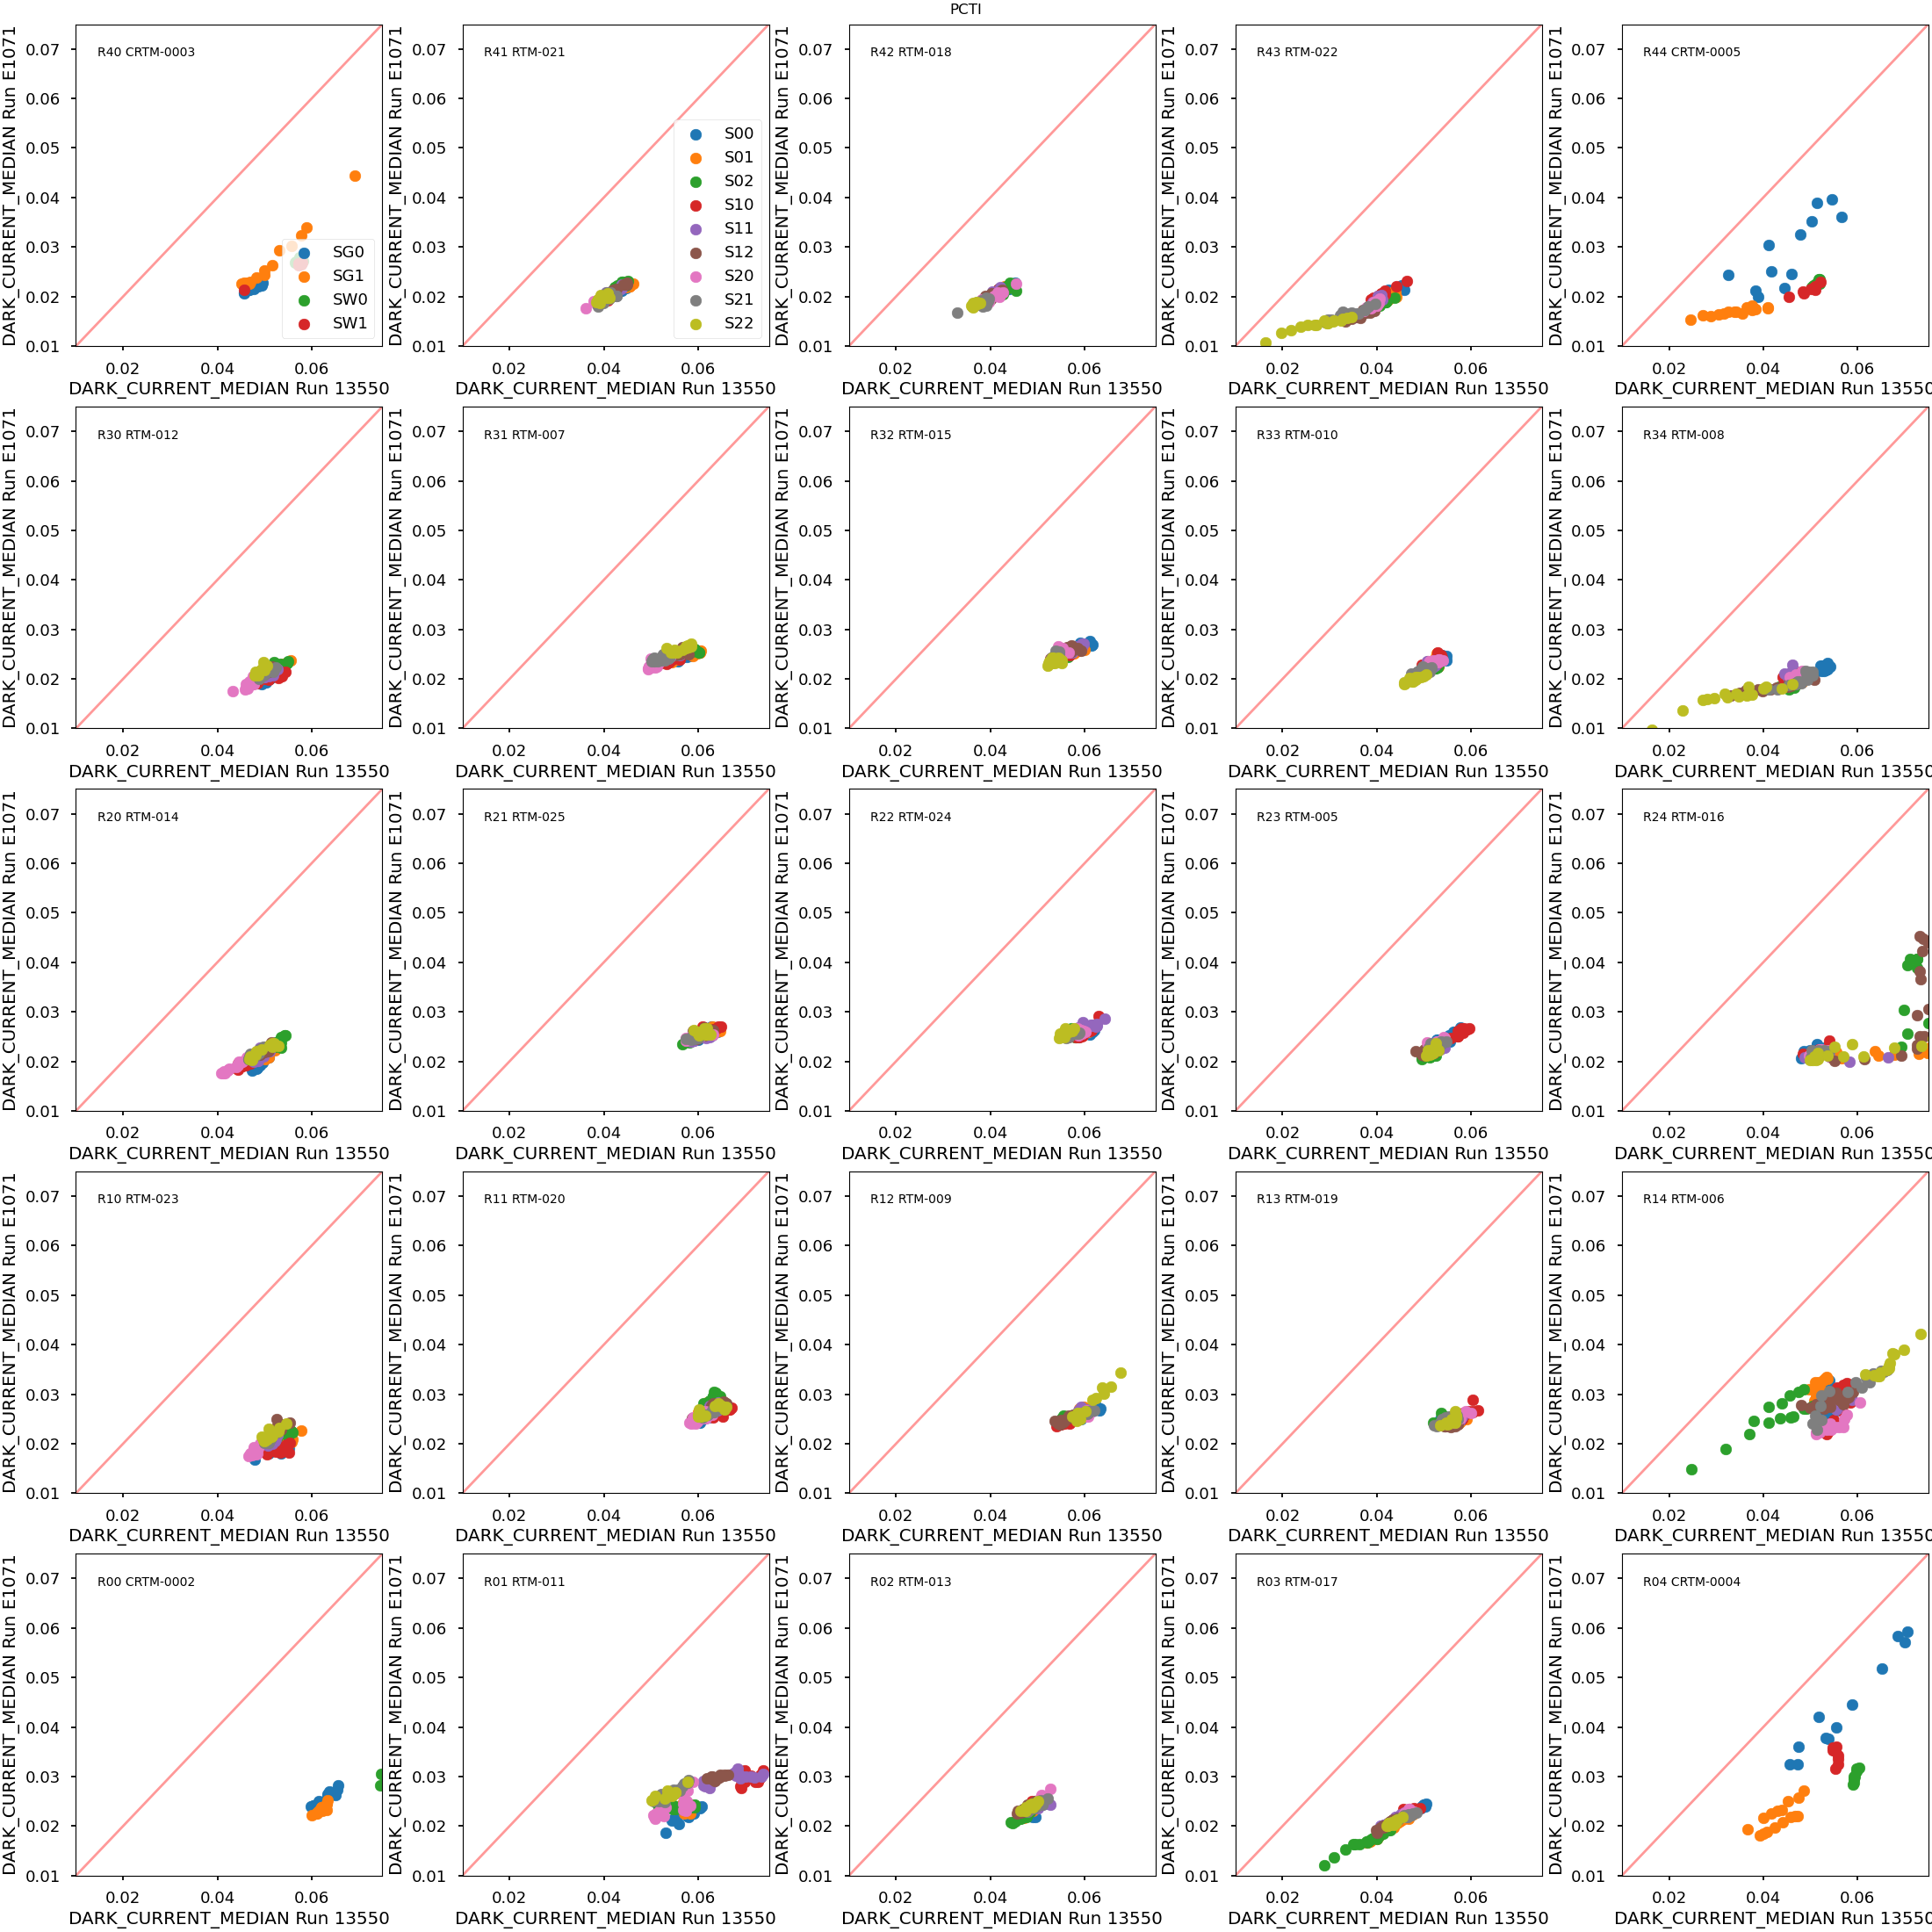
\includegraphics[width=0.7\textwidth]{figures/baselineCharacterization/13550_E1071_DARK_CURRENT_MEDIAN_inset.png}
\caption{Dark current comparison by raft for Run 7 (E1071) and Run 6 (13550).}
\label{fig:dark}
\end{centering}
\end{figure}

Unexpectedly, the dark current was significantly less in Run 7 than
Run 6 (Fig.~\ref{fig:dark}). We do not attach particular significance to the finding because this could be the result of improved shrouding on the camera in the Level 3 white room relative to the IR2 clean room SLAC.

\clearpage
\subsubsection{Bright defects}\label{bright-defects}

Bright defects are localized regions or individual pixels that produce abnormally high signal levels, even in the absence of light. These defects are typically caused by imperfections in the semiconductor material or manufacturing process of the CCD. Bright defects can manifest as ``hot pixels" with consistently high dark current, small clusters of pixels with elevated dark current, or as ``hot columns" (pixels along the same column that have high dark current). 

In the context of LSST Camera, we identify and exclude bright pixels from the dark current measurement, with the threshold for a bright defect set at 5 e$^-$/pix/s, above which the pixel/cluster/column is registered as a bright defect. In addition to the bright pixel metric, eo-pipe also computes a bright column metric, which is any region of bright pixels that is contiguous over 50 pixels or more.

\begin{figure}[ht]
\begin{centering}
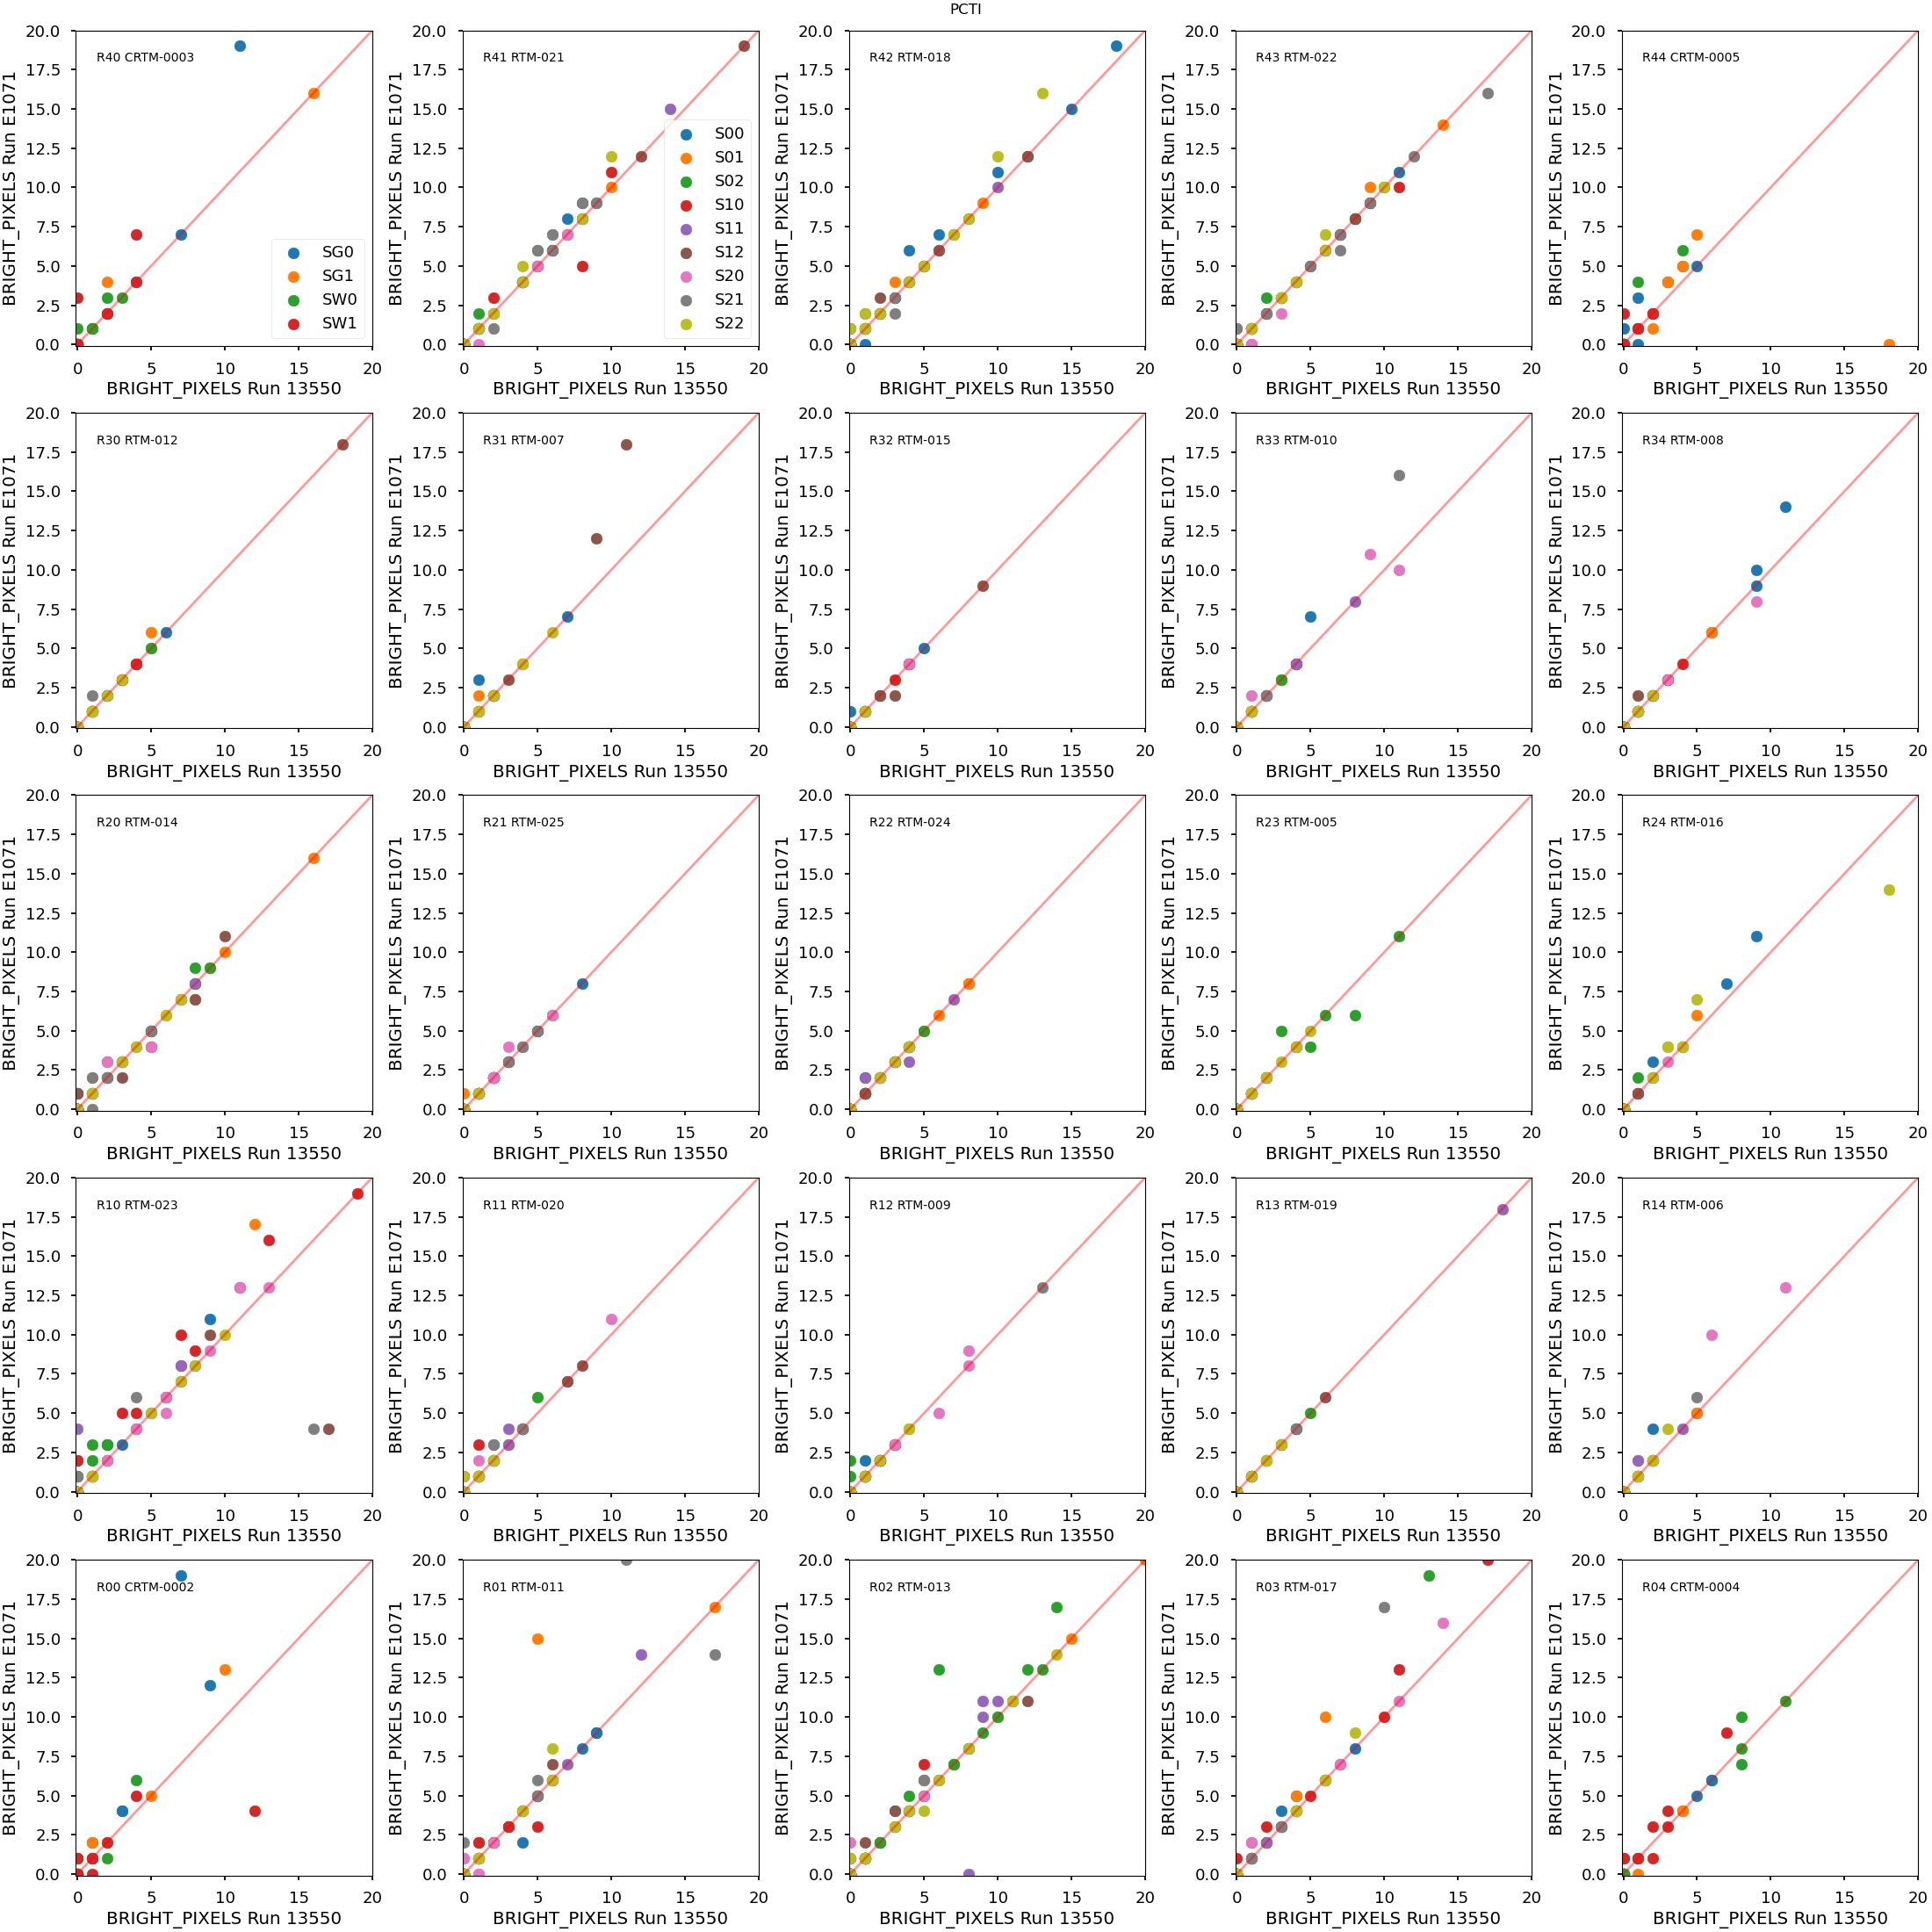
\includegraphics[width=0.7\textwidth]{figures/baselineCharacterization/13550_E1071_BRIGHT_PIXELS_inset.png}
\caption{Bright pixel comparison by raft for Run 7 (E1071) and Run 6 (13550)}
\label{fig:bright}
\end{centering}
\end{figure}

Evaluating the change in defect counts on each amplifier segment between Run 6 and Run 7, and aggregating the amplifiers by the detector manufacturer shows a small increase of bright defects in Run 7 (Fig.~\ref{fig:bright}). Figure~\ref{fig:dark-dist}) displays differences of the measurements. The median values agree well, while there are signs of the positive tail. For ITL sensors, we find that 12\% of the amplifiers have more bright pixels than in Run 6. For e2v sensors, we find 4\% of the amplifiers that have more bright pixels. Despite this, the number of bright defects between runs does not increase for most sensors.

The reason is not totally clear, but the difference in the illumination pattern as described in Section \ref{run-7-optical-modifications} might play a role, which implies that a small number of defects could be created in the CCOB optical path.

\begin{figure}[ht]
\begin{centering}
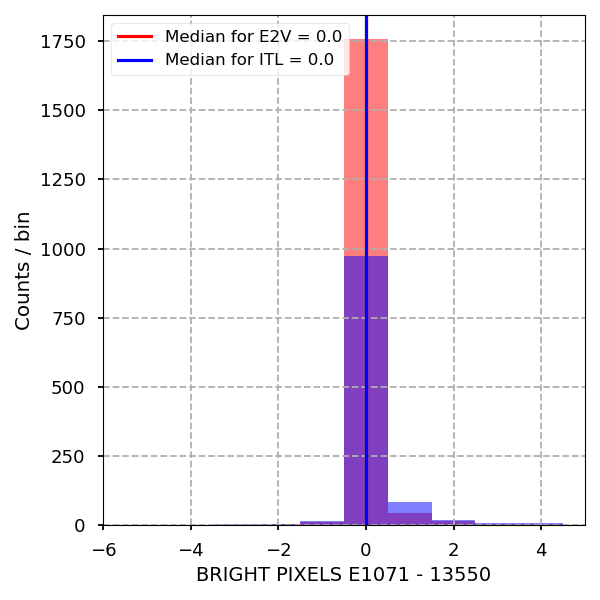
\includegraphics[width=0.7\textwidth]{figures/baselineCharacterization/BRIGHT_PIXELS_13550_E1071_diff.png}
\caption{Distributions of differences in bright pixel count per amplifier between Run 7 (E1071) and Run 6 (13550), grouped by CCD type.}
\label{fig:dark-dist}
\end{centering}
\end{figure}

\clearpage
\subsection{Flat pair metrics}\label{flat-pair-metrics}

\begin{figure}[ht]
\begin{centering}
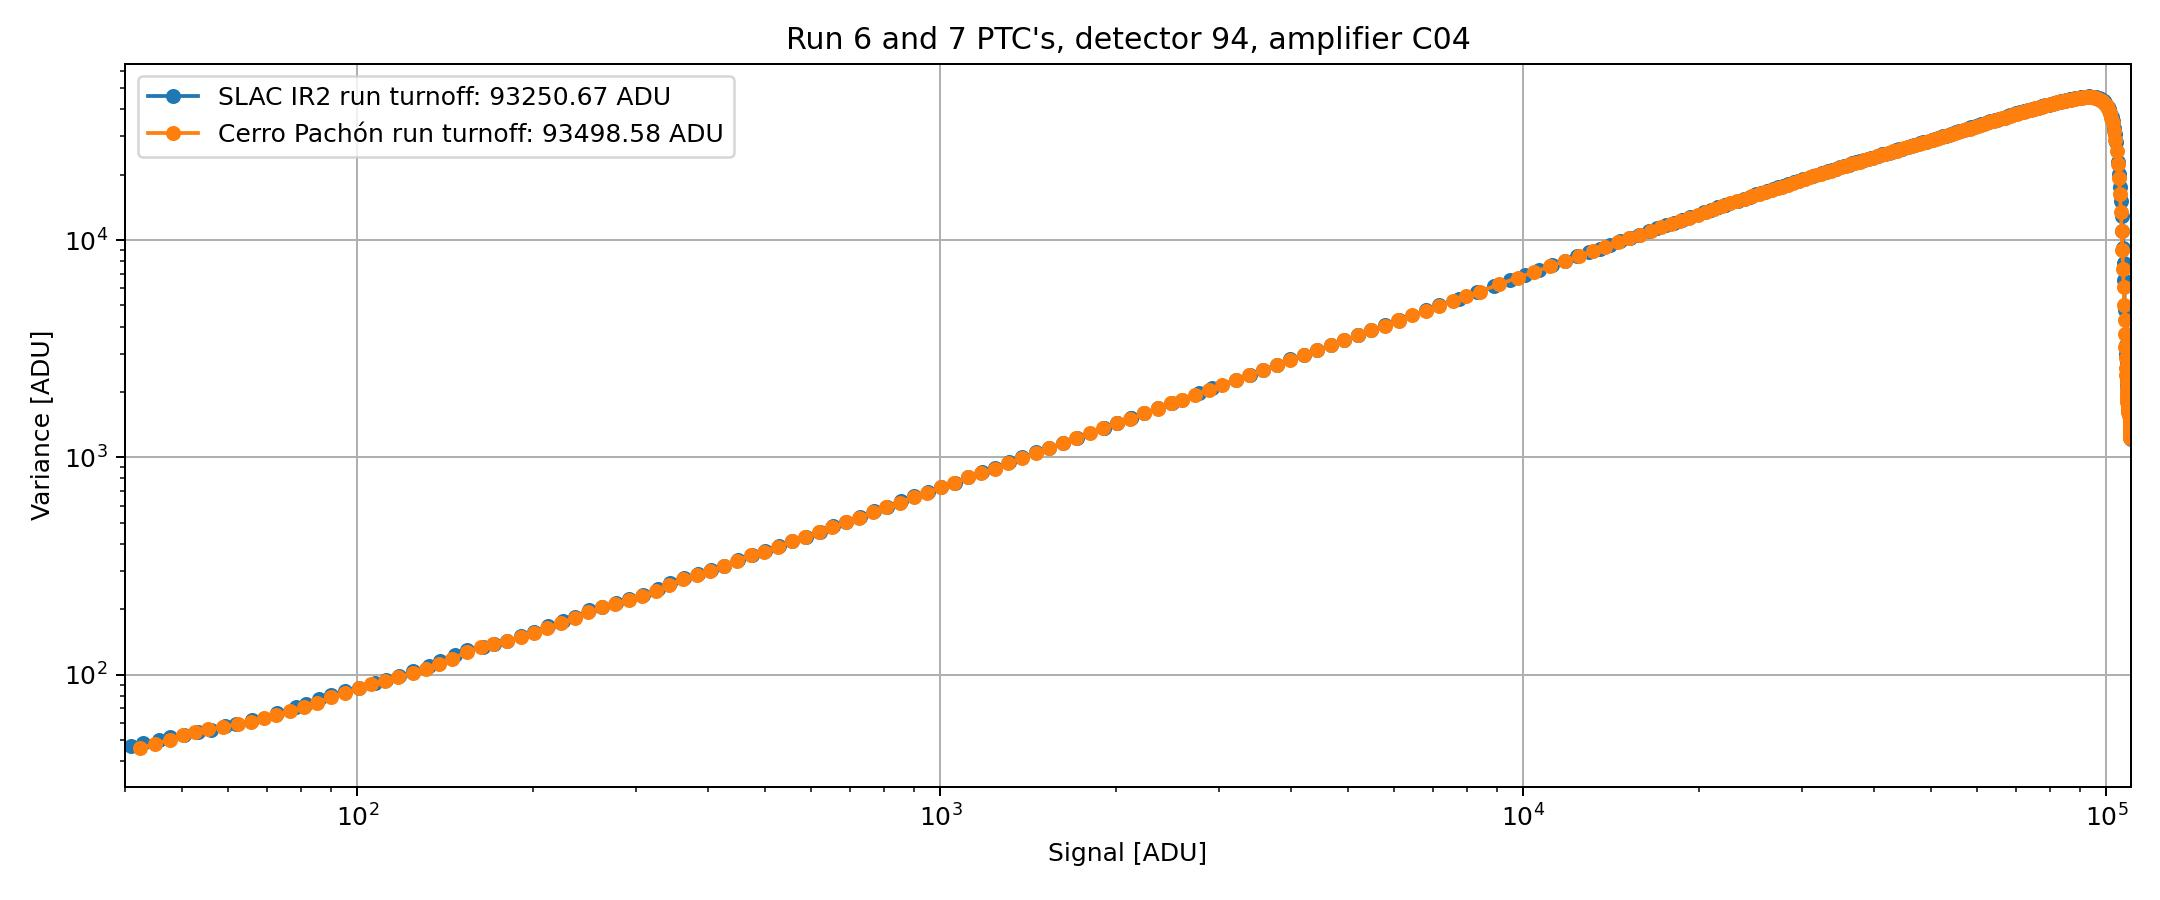
\includegraphics[width=0.95\textwidth]{figures/baselineCharacterization/run7PTCsToDate.jpg}
\caption{A comparison of Run 6 and Run 7 PTCs for a central amplifier.}
\label{fig:initRever:PTC_Comparison}
\end{centering}
\end{figure}

\clearpage
\subsubsection{Linearity and PTC turnoff}\label{linearity-and-ptc-turnoff}

Linearity turnoff and PTC turnoff are two closely related metrics used
to characterize the upper limit of the usable signal range for accurate shape measurements and photometry. Linearity turnoff is the signal level above which the PTC curve deviates from
linearity and is measured for each amplifier segment of each CCD. We have defined the deviation threshold as 2\%.
PTC turnoff refers to the high-signal region of the PTC above which the PTC
variance decreases with increasing signal. This is due to saturation within the pixel wells of the CCDs. While slightly different, both metrics
provide important information about the upper limits of the dynamic
range in our sensors. Linearity turnoff is measured in units of e$^-$,
while PTC turnoff is measured in ADU.

\begin{figure}[ht]
\begin{centering}
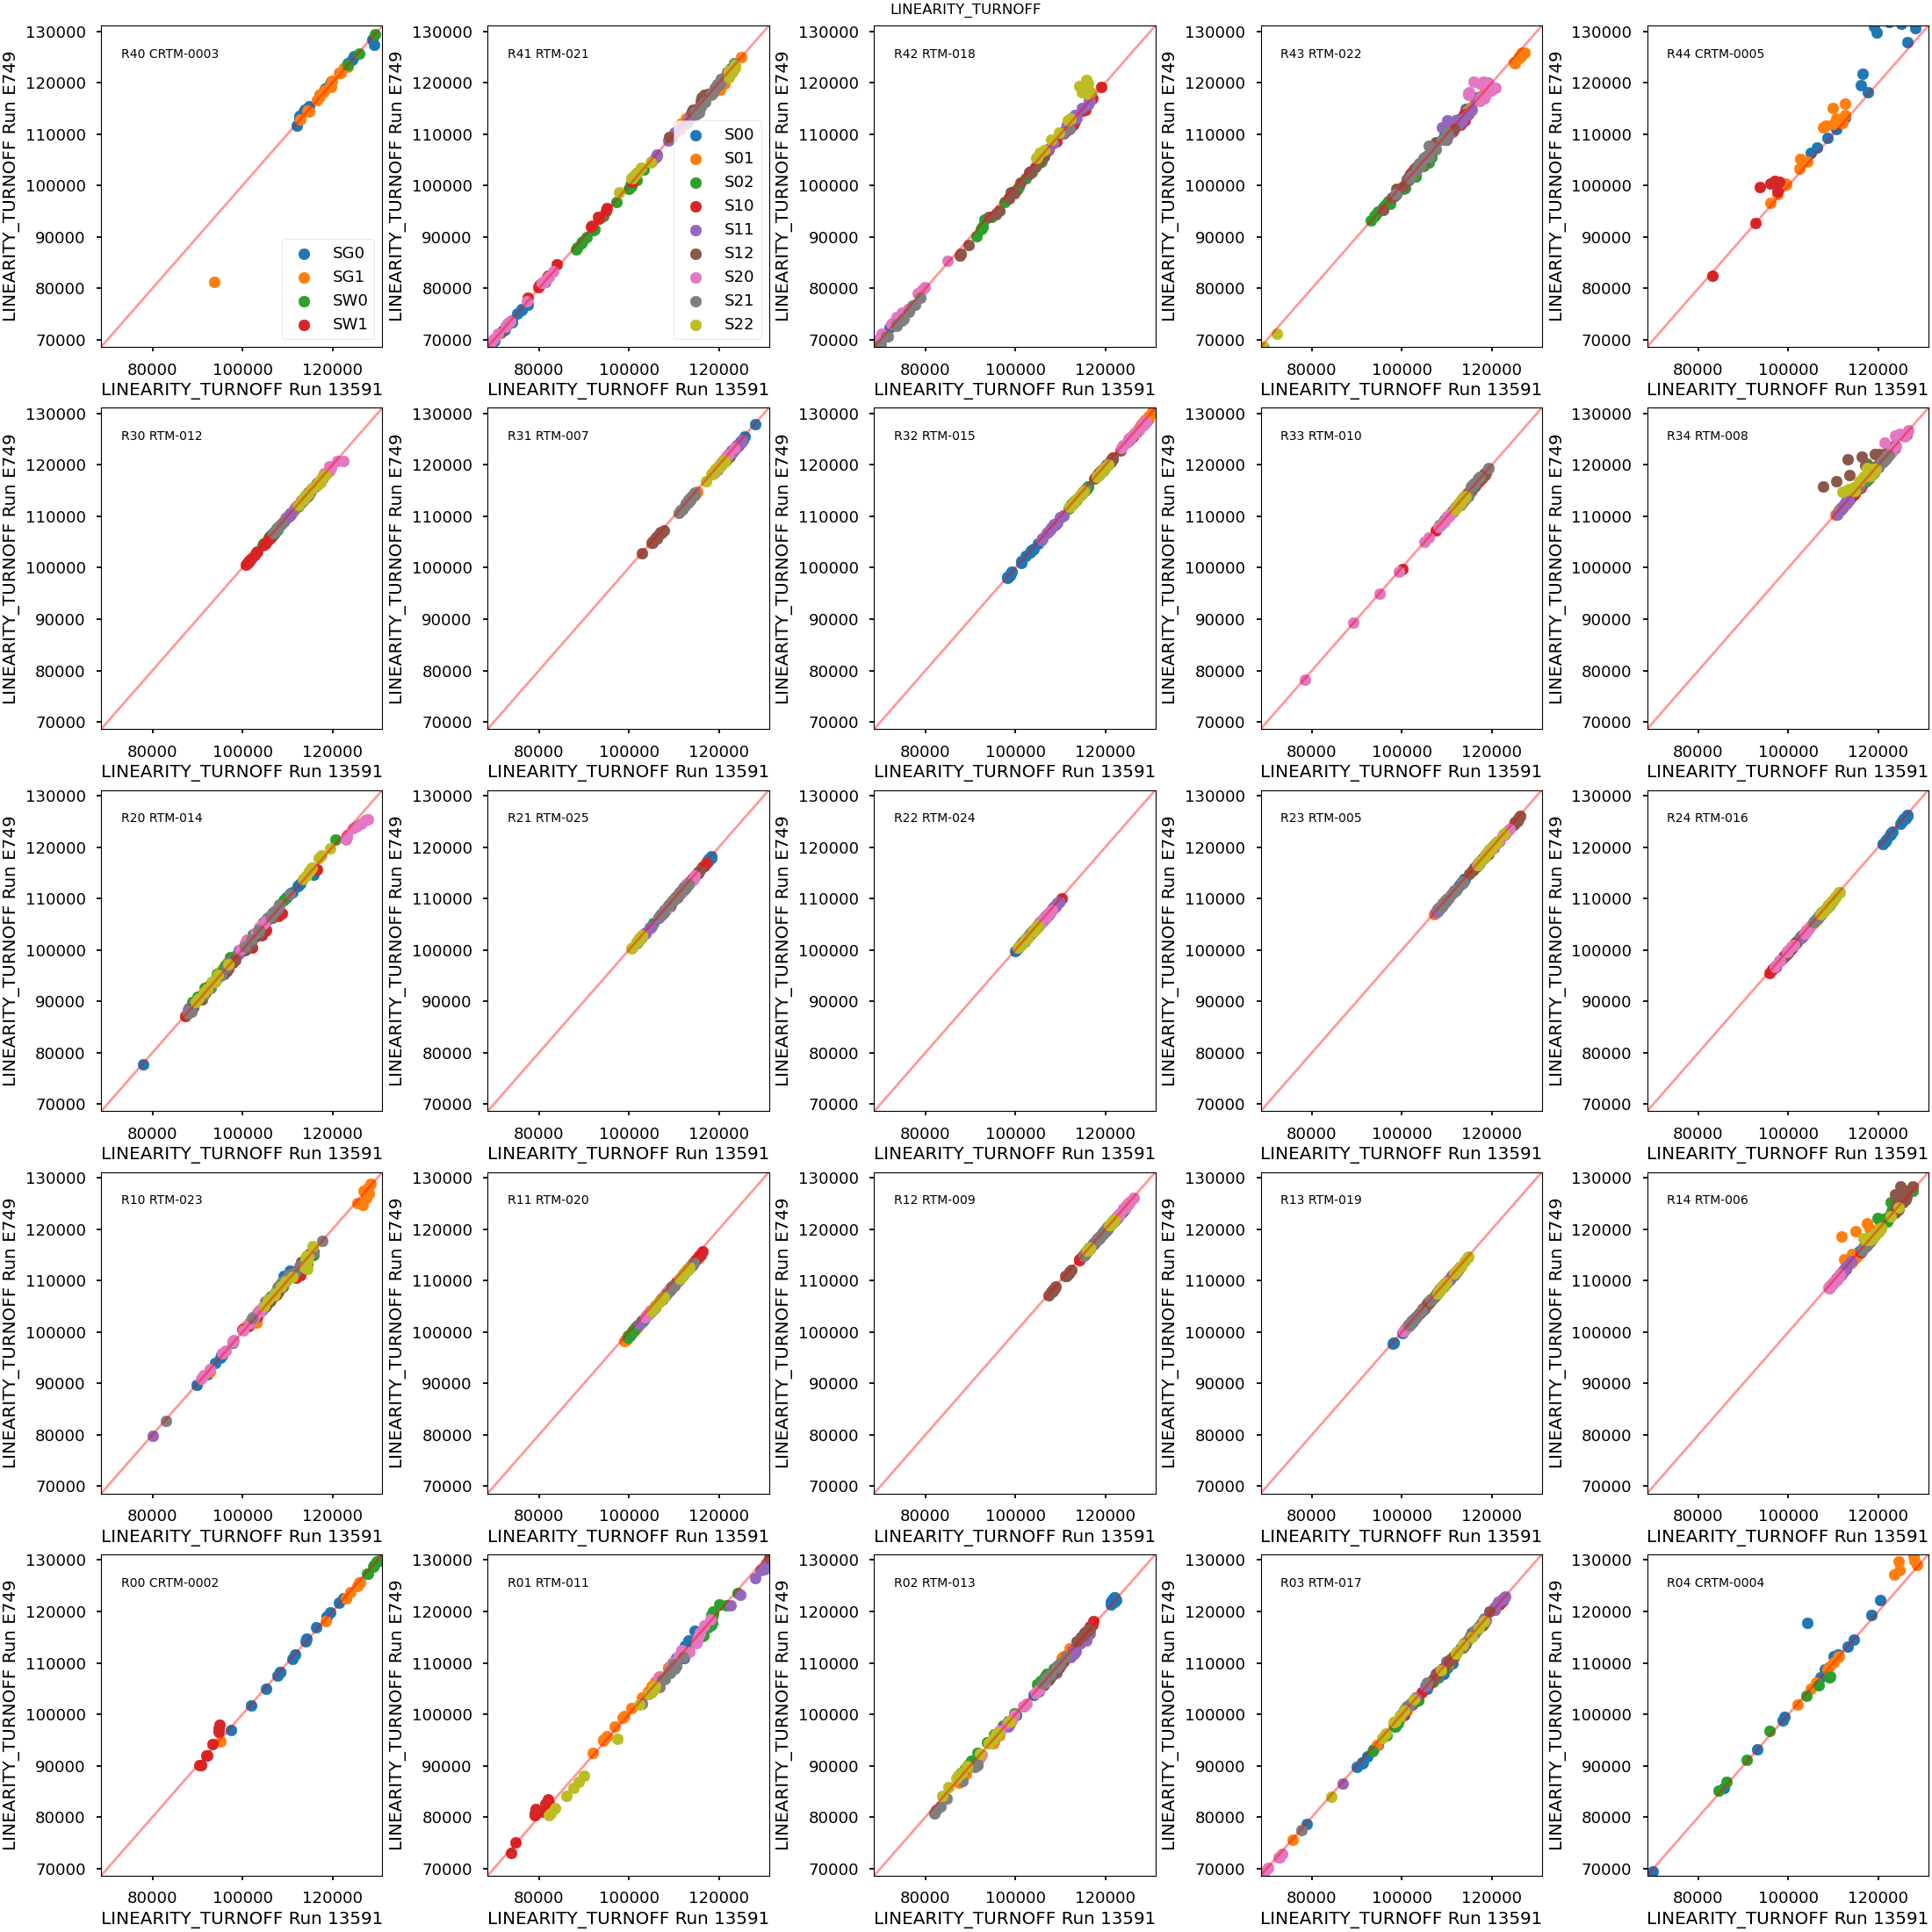
\includegraphics[width=0.7\textwidth]{figures/baselineCharacterization/13591_E749_LINEARITY_TURNOFF.png}
\caption{A comparison of Run 7 amplifier measurements of linearity turnoff, separated by sensor type. For both sensor types, measurements agree across both runs.}
\end{centering}
\end{figure}

In our linearity turnoff measurements, we find close agreement between
our Run 7 and Run 6 measurements for both ITL and e2v sensors.

\begin{figure}[ht]
\begin{centering}
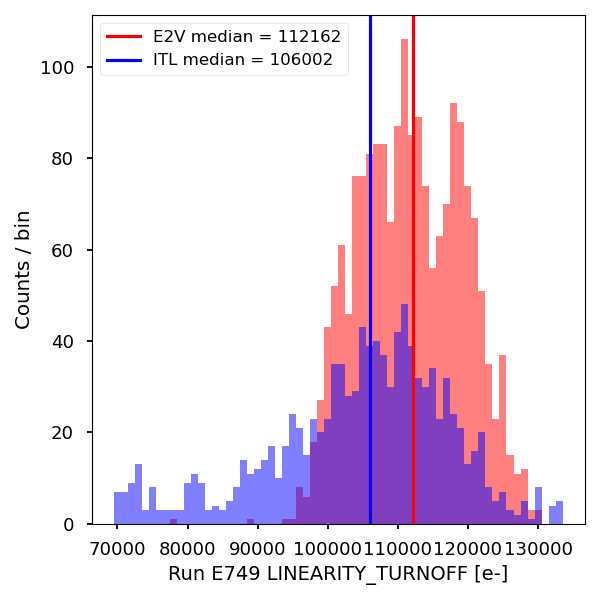
\includegraphics[width=0.7\textwidth]{figures/baselineCharacterization/LINEARITY_TURNOFF_E749_sensorType.png}
\caption{A comparison of Run 7 amplifier measurements of linearity turnoff, separated by sensor type. For both sensor types, linearity turnoff is above the 90k e- specification for a majority of amplifiers. A subset of ITL amplifiers are below the 90k e- threshold, while two e2v amplifiers are below that specification.}
\end{centering}
\end{figure}

Run 7 PTC turnoff measurements agree closely between Run 6 and Run 7, differing by $\leq$ 200 $e^-$ for both ITL and e2v sensors. Notably, they are lower on average for both detector types.

\begin{figure}[ht]
\begin{centering}
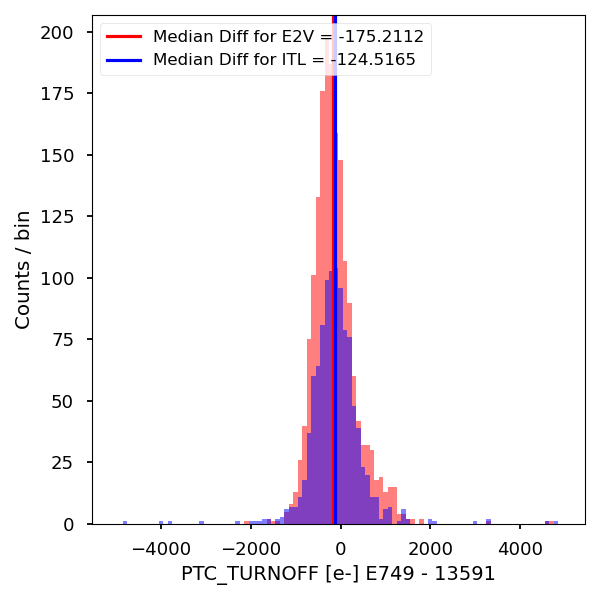
\includegraphics[width=0.7\textwidth]{figures/baselineCharacterization/PTC_TURNOFF_13591_E749_diff.png}
\caption{A comparison of Run 6 and Run 7 amplifier differences in PTC turnoff, separated by sensor type. For both sensor types, PTC turnoff is very consistent.}
\end{centering}
\end{figure}

\clearpage
\subsubsection{PTC gain}\label{ptc-gain}

PTC gain is the conversion factor between digital output signal and the the number of electrons generated in the pixels of the CCD. It is one of the key parameters derived from the Photon Transfer
Curve, as it is the slope above the flux range at which the variance is dominated by shot noise, and below the PTC turnoff. Gain is expressed in e$^-$/ADU, and scales the digitized analog signals from the ASPICs (Application Specific Photonic Integrated Circuits) to units of e$^{-1}$.

\begin{figure}[ht]
\begin{centering}
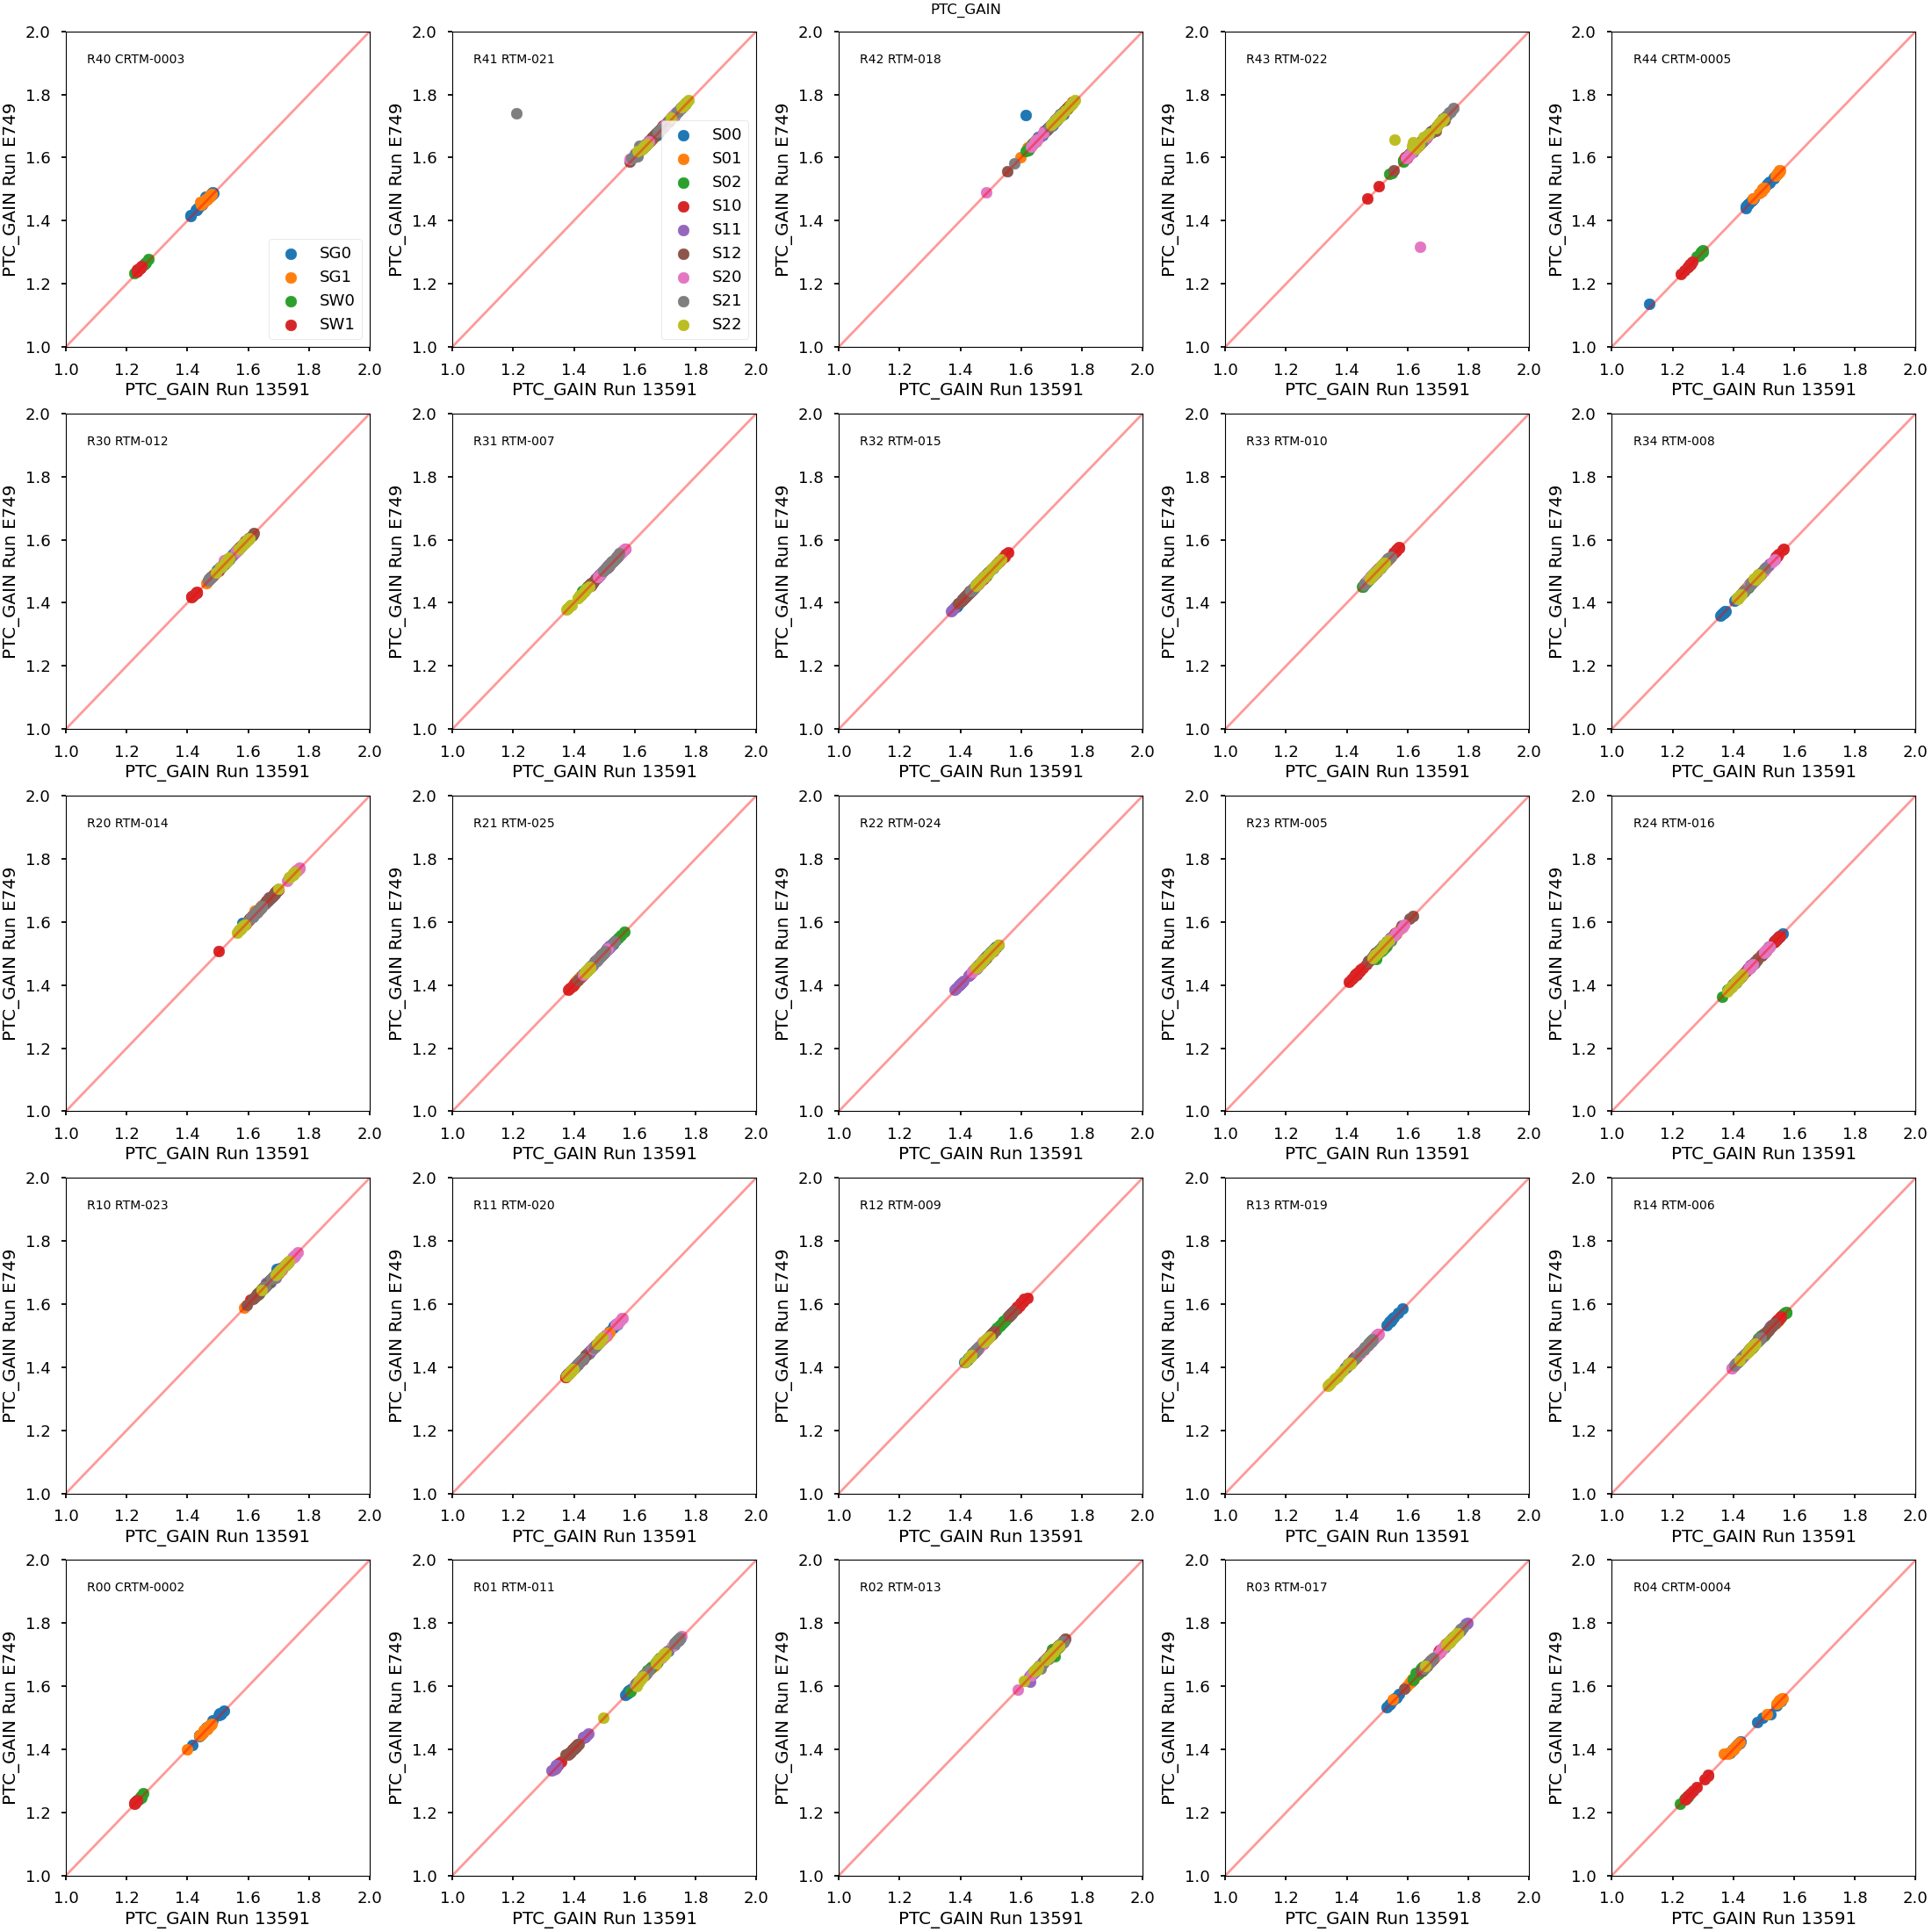
\includegraphics[width=0.7\textwidth]{figures/baselineCharacterization/13591_E749_PTC_GAIN.png}
\caption{A comparison of Run 6 and Run 7 amplifier measurements in gain, separated by sensor type. For both sensor types, gain is very consistent.}
\end{centering}
\end{figure}

PTC gain measurements agree extremely closely across all sensors in the
focal plane.

\clearpage

\subsubsection{Read Noise}\label{sec:initialRever:ReadNoise}

Read noise is induced charge during the readout process of the LSST Camera sensors. Common causes of read noise include thermal noise in the electronics or imperfect charge transfer. Read noise is measured in electrons, and is calculated by taking the standard deviation of the overscan region.

\begin{figure}[ht]
\begin{centering}
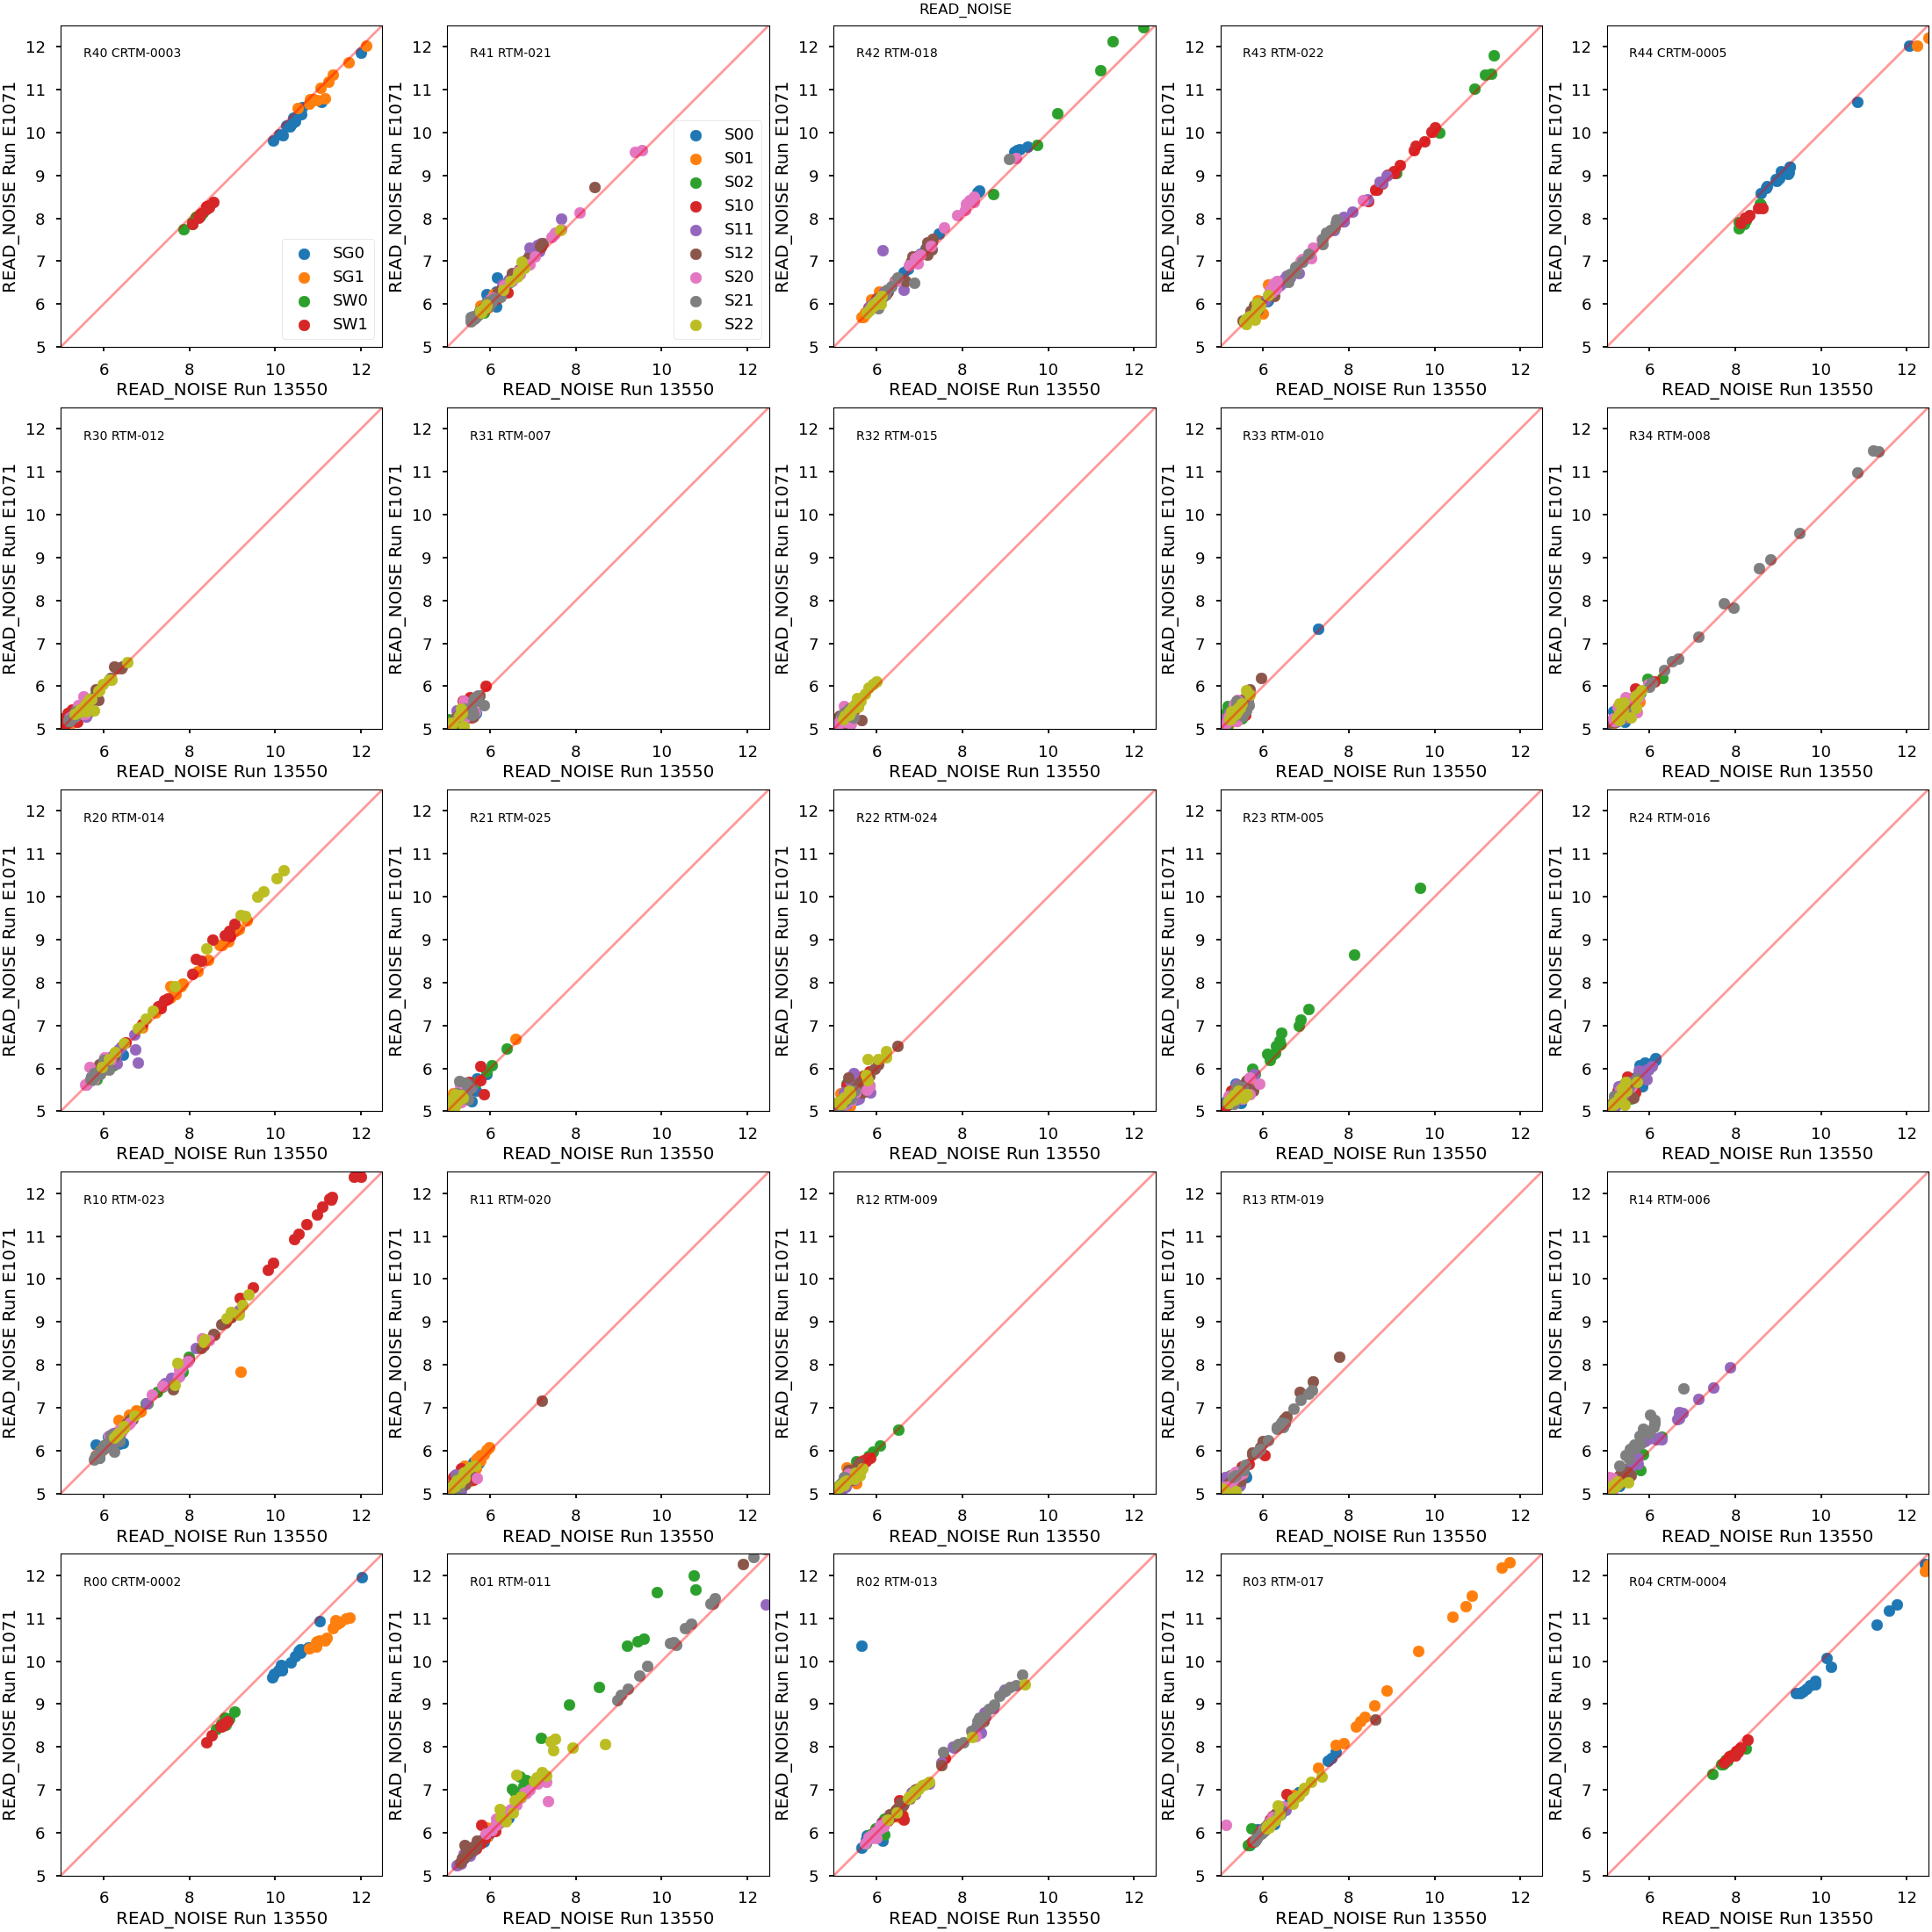
\includegraphics[width=0.7\textwidth]{figures/baselineCharacterization/13550_E1071_READ_NOISE_inset.png}
\caption{A comparison of Run 6 and Run 7 amplifier measurements for read noise, separated by sensor type. For both sensor types, read noise is higher in Run 7.}
\end{centering}
\end{figure}

The read noise is higher in Run 7 than Run 6 for both sensor types. The difference is on the order of 0.05 e-.

\begin{figure}[ht]
\begin{centering}
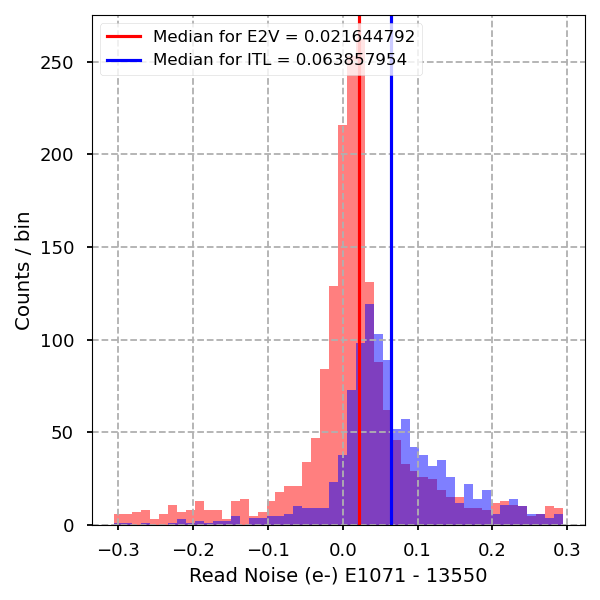
\includegraphics[width=0.7\textwidth]{figures/baselineCharacterization/ReadNoisee-_13550_E1071_diff.png}
\caption{A comparison of Run 6 and Run 7 amplifier measurements for read noise, separated by sensor type. For both sensor types, read noise is higher in Run 7.}
\end{centering}
\end{figure}

\subsubsection{PTC Noise}\label{sec:initialRever:PTCNoise}

PTC noise is a fitted parameter in the PTC model, and is the foundation of the PTC model. In the shot noise regime, where the PTC slope is 1/2 in log-log space (from 500 - 10k ADU in figure \ref{fig:initRever:PTC_Comparison}), the data can be fitted to a line. The intercept of that line is the PTC noise, measured in ADU.

\begin{figure}[ht]
    \centering
    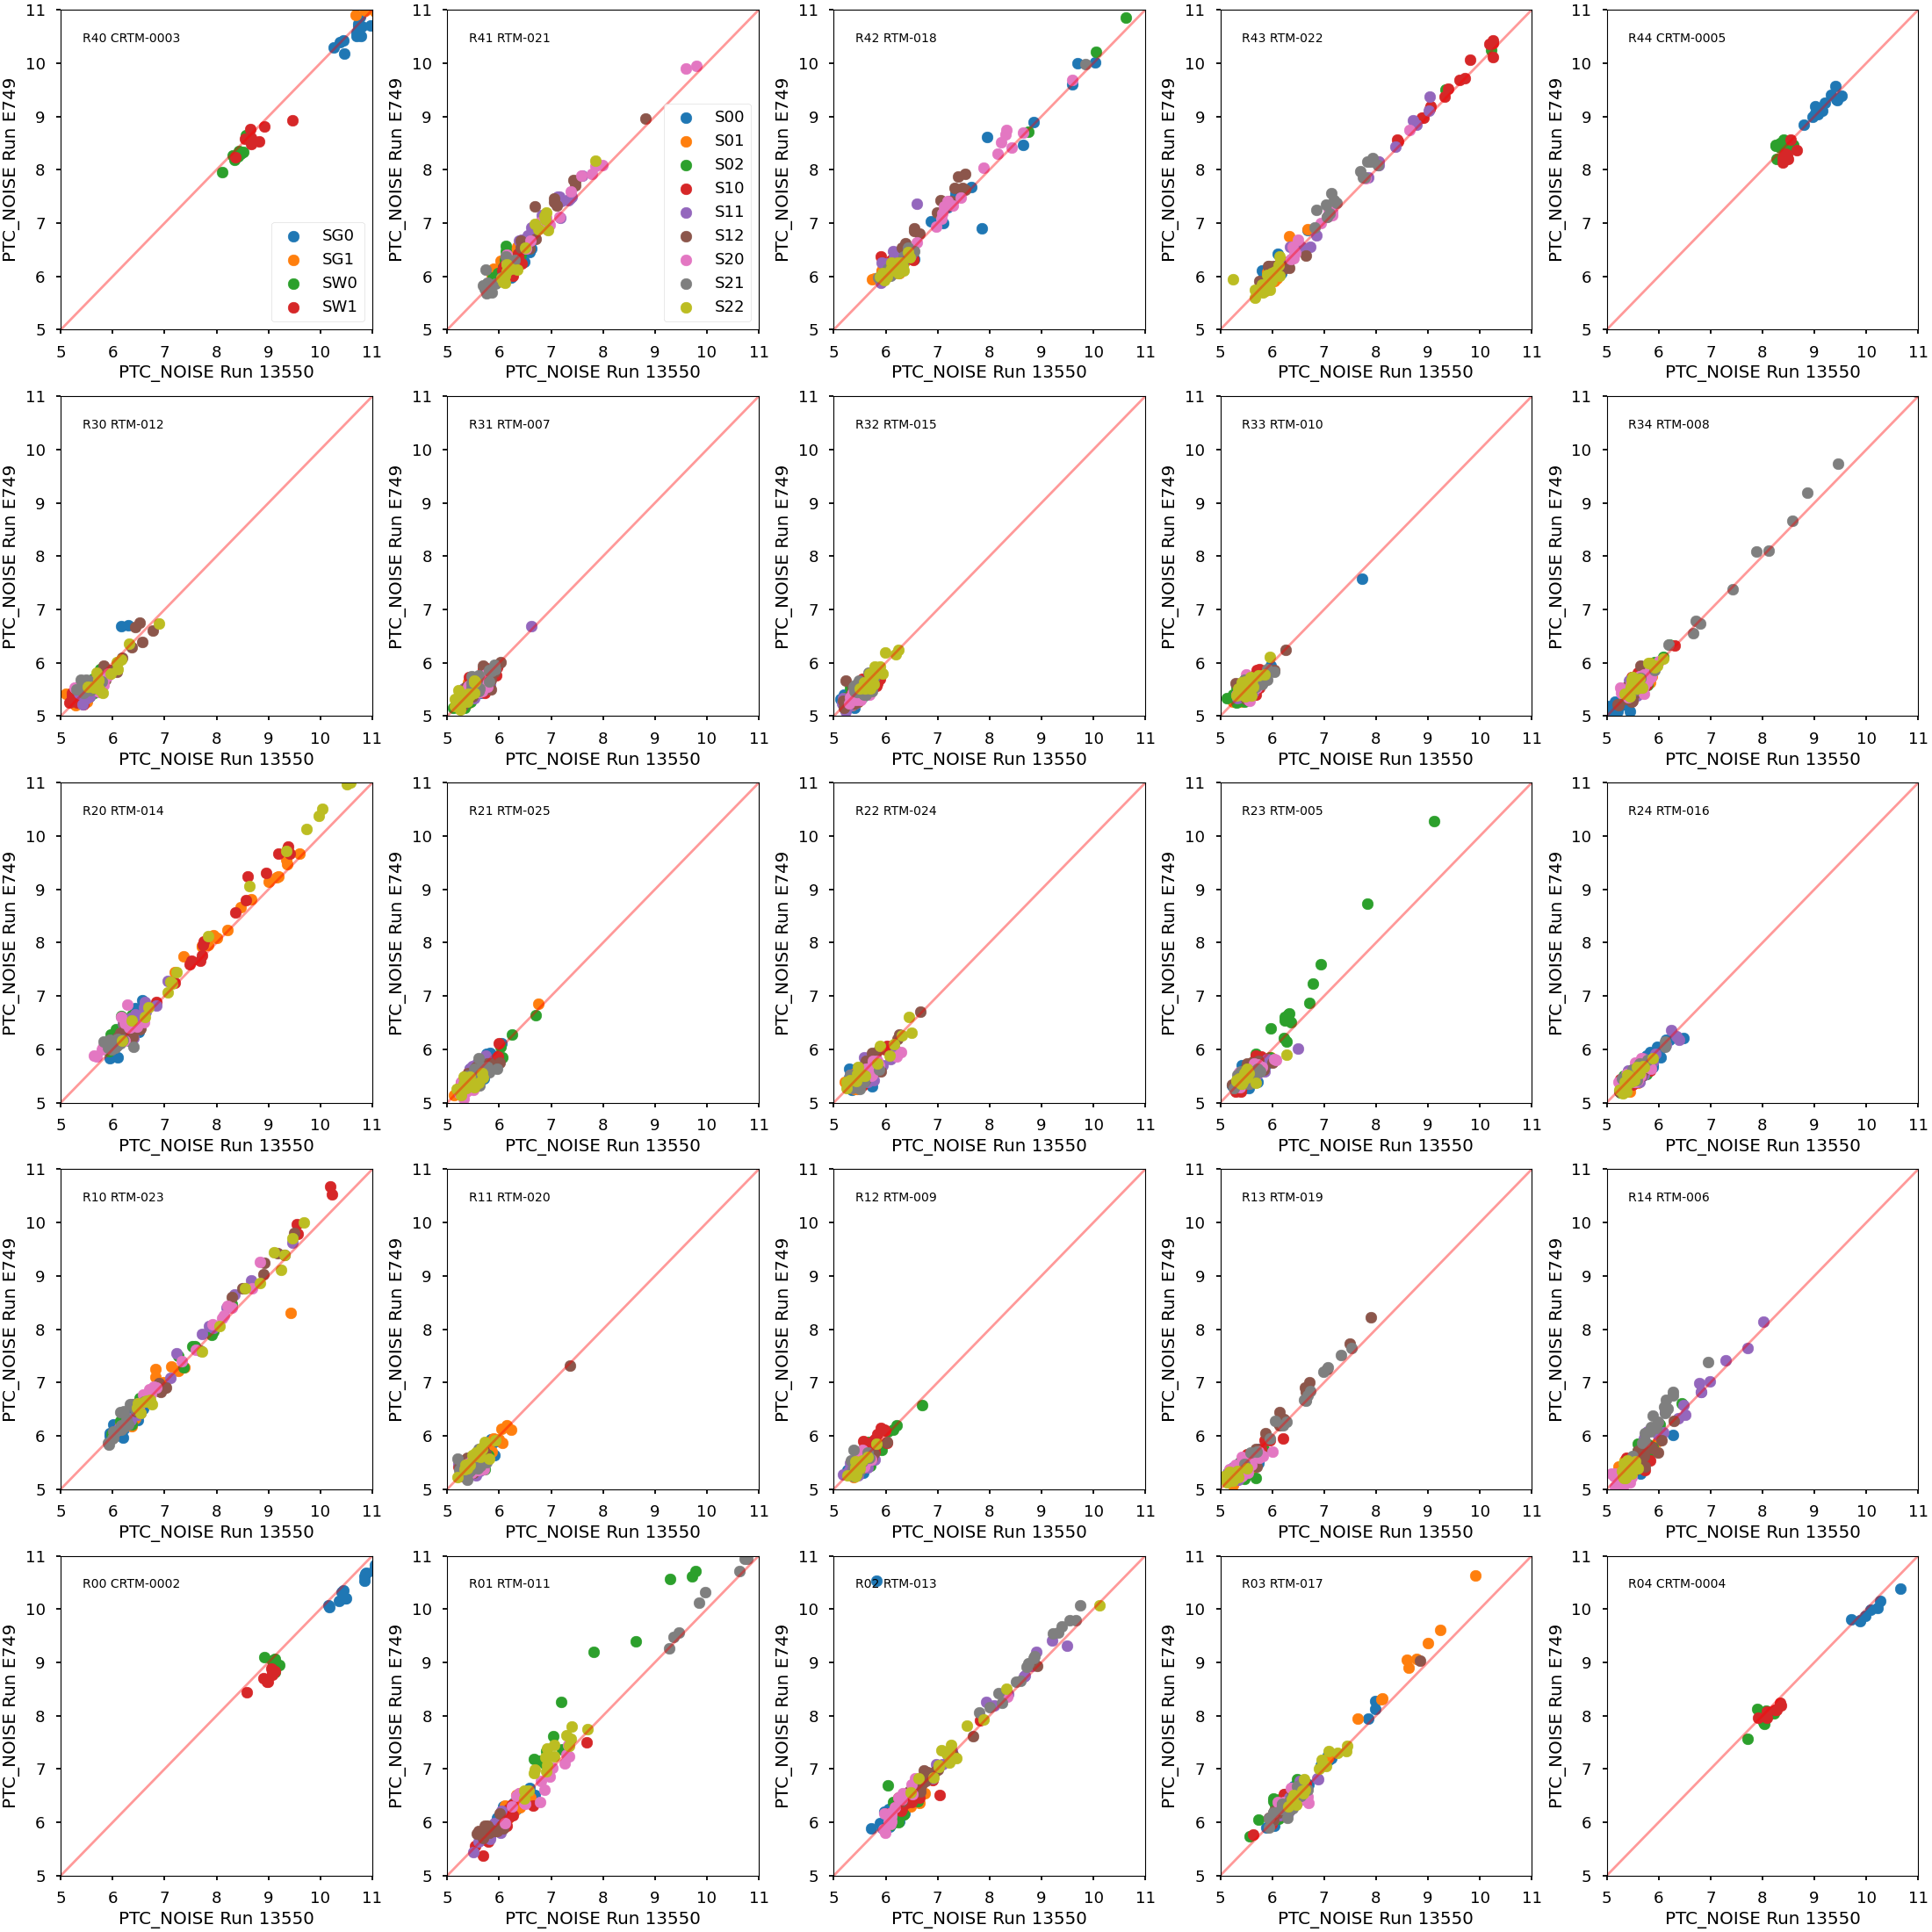
\includegraphics[width=0.7\linewidth]{figures/baselineCharacterization/13550_E749_PTC_NOISE.png}
    \caption{Comparison of amplifier measurements of PTC noise for initial and final Run 7 conditions.}
    \label{fig:initRever-PTC_NOISE_5x5}
\end{figure}

PTC noise differs by $\lesssim$ 0.1 e- on average for science sensors. Notably, e2v sensors measure a PTC noise 0.02 e- lower in Run 7, while ITL sensors measure a PTC noise 0.08 e- higher in Run 7 (see figure \ref{fig:initRever:PTCNoise_hist_diff}).

\begin{figure}[ht]
    \centering
    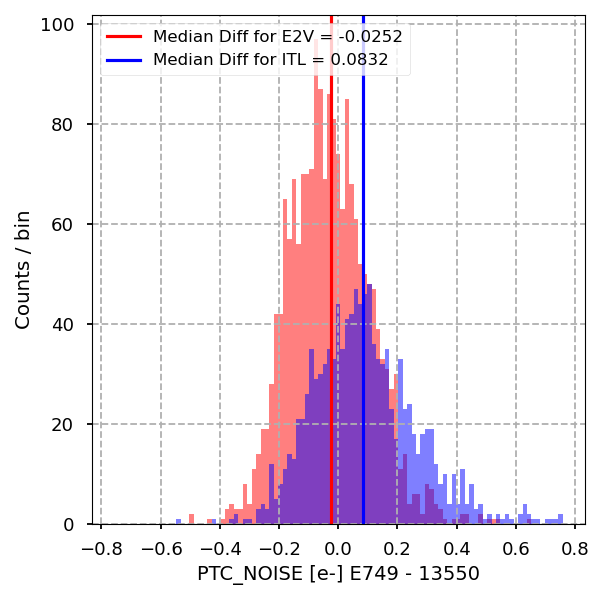
\includegraphics[width=0.7\linewidth]{figures/baselineCharacterization/PTC_NOISE_13550_E749_diff.png}
    \caption{Comparison of the PTC noise measurements in different sensors and run types.}
    \label{fig:initRever:PTCNoise_hist_diff}
\end{figure}


\subsubsection{Brighter-fatter coefficients}\label{brighter-fatter-a00-coefficient}


The brighter-fatter effect in CCDs refers to the phenomenon where brighter sources appear larger (or ``fatter" than dimmer ones). This occurs due to electrostatic interactions within the pixel wells of the CCDs, when a pixel accumulates a high charge from incoming photons and creates an electric field that slightly repels incoming charge carriers into neighboring pixels. The brighter-fatter effect can be modeled as the most dominant source of pixel-pixel correlations. Following the PTC model from  
\citet{2019A&A...629A..36A}, $a_{00}$ describes the change of a pixel area due to its own charge content, or the relative strength of the brighter-fatter effect. Since same-charge carriers repel each other, the pixel area decreases as charge accumulates inside the pixel well, which implies $a_{00}$ \textless{} 0. Similarly $a_{10}$ describes the area change cause by a pixel to its nearest serial neighbor, and $a_{01}$ to the parallel nearest neighbor. Figs. \ref{fig:hist_as_run6_7} and \ref{fig:ratio_bf_coeff_6_7} compare the measurement of these coefficients carried out at SLAC and at the summit. We see that the variations are modest (and could be explained by noise) except for two rafts: R10 and R11. The Run 6 data used for this comparison was acquired with a high voltage of 45V applied to these two rafts, rather than the usual 50\,V. The sensitivity of our measurements of the brighter-fatter coefficients is sufficient to detect the change of electrostatic conditions due to this change of drift field in the sensors. In {\tt eo\_pipe}, an absolute value is taken of the $a_{00}$ parameter, so the tabulated quantities are positive.

\begin{figure}[ht]
    \begin{centering}
  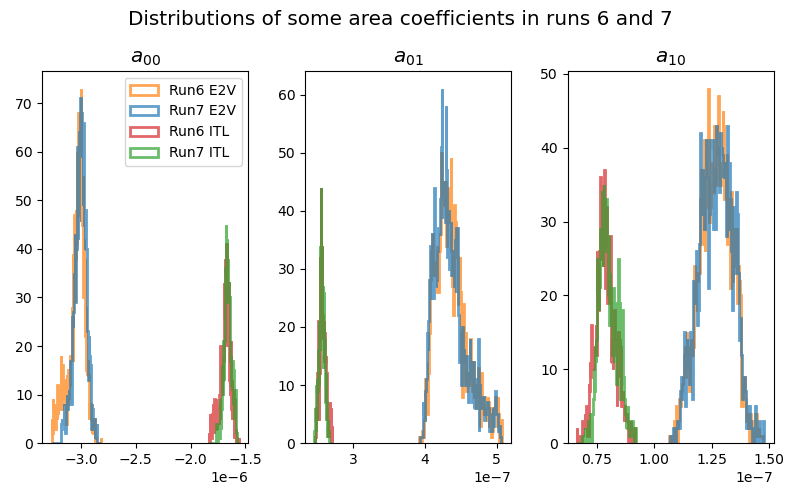
\includegraphics[width=0.7\linewidth]{figures/hist_as_run6_7.png}

  \caption{Distributions of $a_{00}$, $a_{01}$ and $a_{10}$ in Run 6 and Run 7. Those are very similar, except for two rafts, which had a lower drift electric field (45\,V vs. 50\,V) in Run 6. The ratios are displayed in Figure~\ref{fig:ratio_bf_coeff_6_7}.\label{fig:hist_as_run6_7}}
  \end{centering}
  \end{figure}

\begin{figure}[ht]
  \begin{centering}
   \minipage{0.32\textwidth}
  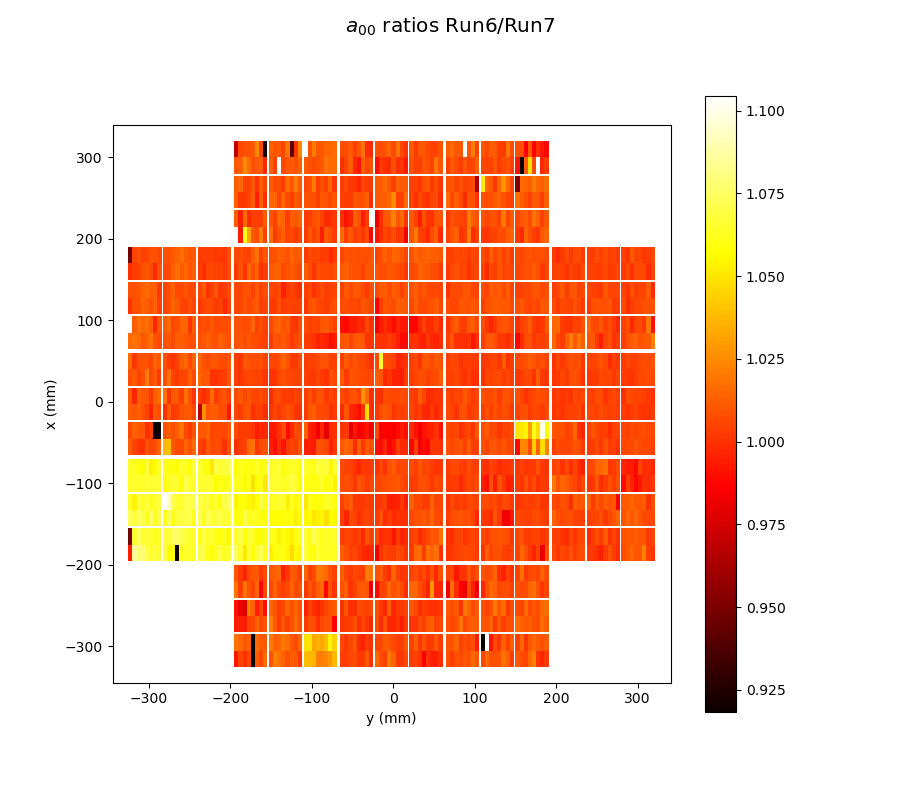
\includegraphics[width=\linewidth]{figures/baselineCharacterization/a00_ratios.png}
  \endminipage\hfill
   \minipage{0.32\textwidth}
  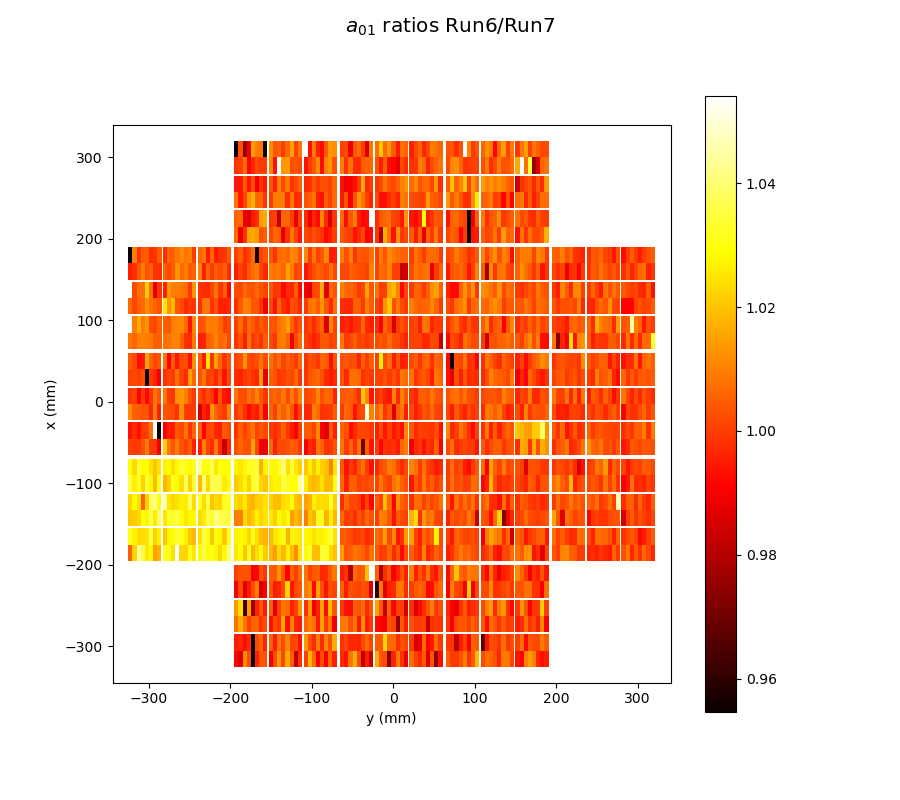
\includegraphics[width=\linewidth]{figures/baselineCharacterization/a01_ratios.png}
  \endminipage\hfill
   \minipage{0.32\textwidth}
  \includegraphics[width=\linewidth]{figures/baselineCharacterization/a10_ratios.png}
  \endminipage\hfill
  

\caption{Ratio of measurements of $a_{00}$, $a_{01}$ and $a_{10}$ coefficients (one per amplifier) for Run 6 and Run 7. They are very consistent, except for two rafts (R10 and R11) where the high voltage was changed between the two runs.\label{fig:ratio_bf_coeff_6_7}}
  \end{centering}
  \end{figure}

The distribution of the difference of $a_{00}$ measurements between the runs is displayed in Figures~\ref{fig:ptc_a00_diff_hist} and \ref{fig:ptc_a00_5x5}.

\begin{figure}[ht]
\begin{centering}
\includegraphics[width=0.7\textwidth]{figures/baselineCharacterization/13591_E749_PTC_A00.png}
\caption{Comparison of Run 6 and Run 7 amplifier differences in the $a_{00}$ coefficient, separated by amplifier across the focal plane. The amplifiers associated with R10 and R11 are noted outliers, as seen in figure \ref{fig:ratio_bf_coeff_6_7}.}
\label{fig:ptc_a00_5x5}
\end{centering}
\end{figure}

\begin{figure}[ht]
\begin{centering}
\includegraphics[width=0.7\textwidth]{figures/baselineCharacterization/PTC_A00_13591_E749_diff.png}
\caption{A comparison of Run 6 and Run 7 amplifier differences in the $a_{00}$ coefficient, separated by sensor type. For both sensor types, the $a_{00}$ coefficient is very consistent. The two peaks on the left represent the two outlier rafts visible on Figure \ref{fig:ratio_bf_coeff_6_7}. The $a_{00}$ values are of the order of 2 to 3 $10^{-6}\ e^{-1}$. \label{fig:ptc_a00_diff_hist}}
\end{centering}
\end{figure}

However, the differences in the brighter-fatter $a_{00}$ coefficient between Run 6 and Run 7 show that the magnitude of $a_{00}$ decreased for most of the outliers, which implies an improvement in imaging for those pixels.

\clearpage
\subsubsection{Row-means variance}\label{row-means-var}

Row-means variance is a metric that measures the mean row-to-row variance of differences between a pair of flats. By computing variance of means of differenced rows at each flux level, we can measure any changes in gain row-by-row and also changes in correlated noise along with row.

\begin{figure}[ht]
\begin{centering}
\includegraphics[width=0.7\textwidth]{figures/baselineCharacterization/13550_E1071_ROW_MEAN_VAR_SLOPE.png}
\caption{A comparison of Run 6 and Run 7 amplifier differences in row-mean-variance slope. For both sensor types, row-means-variance slope is weaker in Run 7. This is more pronounced for e2v sensors.}
\end{centering}
\end{figure}

Differences in row-means variance between runs are evident, and are distinctly different for different detector types. The difference between runs is more significant for ITL sensors, \textasciitilde9\% smaller on average in Run 7. For e2v sensors, the effect is \textasciitilde3\% smaller in Run 7. This indicates that either row-by-row correlated noise or row-by-row gain change is less in Run 6. Since we did not change the sequencer file, the most natural explanation is the row-by-row correlated noise. But further investigation is needed.

\begin{figure}[ht]
\begin{centering}
\includegraphics[width=0.7\textwidth]{figures/baselineCharacterization/ROW_MEAN_VAR_SLOPE_13550_E1071_diff.png}
\caption{A comparison of Run 6 and Run 7 amplifier differences in row-mean-variance slope, separated by sensor type. For both sensor types, row-means-variance slope is weaker in Run 7. This is more pronounced for e2v sensors.}
\end{centering}
\end{figure}

\clearpage
\subsubsection{Divisadero tearing}\label{sec:divisadero:init}

Divisadero tearing (or Rabbit ears) is manifested as signal variations near amplifier boundaries, connected features that are often jagged \cite{2020arXiv200209439J,2024SPIE13103E..0WU}. These variations are on the order of \textasciitilde1\% relative to the flat field signal. To quantify divisadero tearing in a given column, we measure the column signal, and compare it to the mean column signal from flat fields.

\begin{figure}[ht]
\begin{centering}
\includegraphics[width=0.7\textwidth]{figures/baselineCharacterization/13550_E1071_DIVISADERO_TEARING_inset.png}
\caption{A comparison of Run 6 and Run 7 amplifier differences in Divisadero tearing, separated by sensor type. For both sensor types, Divisadero tearing is weaker in Run 7. The difference is more pronounced for e2v sensors, which have larger Divisadero tearing in general.}
\end{centering}
\end{figure}

Divisadero tearing is broadly consistent between Run 6 and Run 7, with both sensor types demonstrating lower Divisadero tearing in Run 7. Taking amplifier differences, e2v sensors show a weaker Divisadero signal in Run 7 by 0.1\%, while ITL sensors demonstrate a weaker Divisadero signal in Run 7 by 0.05\% (see Fig.~\ref{fig:divisadero_diff_baseline}).

\begin{figure}[ht]
    \centering
    \includegraphics[width=0.7\linewidth]{figures/baselineCharacterization/DIVISIDERO_TEARING_13550_E1071_diff.png}
    \caption{A comparison of Run 6 and Run 7 amplifier differences in Divisadero tearing, separated by sensor type. For both sensor types, divisadero tearing is weaker in Run 7.}
    \label{fig:divisadero_diff_baseline}
\end{figure}

\clearpage
\subsubsection{Dark defects}\label{dark-defects}

Dark defects are localized regions or individual pixels that produce abnormally low signal levels, even in the presence of light. Similarly to bright pixels, dark pixels are also quantified in dark columns over 50 pixel contiguous regions. These
defects are caused by imperfections in the semiconductor
material, imperfections during the manufacturing process of a CCD. For our evaluation, we extract dark pixels from combined flats, with the threshold for a dark defect defined as a $-$20\% deficit from the average flat field flux measured in the image segment.

\begin{figure}[ht]
\begin{centering}
\includegraphics[width=0.7\textwidth]{figures/baselineCharacterization/detector_85.jpg}
\caption{Illustration of masked border pixels (yellow) for detector 85 (R21\_S11). The average defect mask size is 4 pixels along the serial (x-pixel) direction, and 5 pixels along the parallel direction. Additional dark defects exist in the sensor, but are difficult to quantify due to the overwhelming contribution from the picture frame response.}
\label{fig:fig-edge-mask}
\end{centering}
\end{figure}

%%
The eo-pipe configuration for evaluating dark defects considers a border pixel region that is masked differently from the dark pixels. The default size for this edge is zero pixels. With a zero pixel border mask, the average dark defect count is 1800 per amplifier, with \geq 95\% of the contribution coming from the picture frame. The `picture-frame response' (also called `edge roll-off') near the edges of the sensors is due to a decrease in the pixel active area. It is difficult to extract useful information about the dark defects in the focal plane without excluding the picture frame. The effects of the picture frame signal on dark defect masking is shown in figure~\ref{fig:fig-edge-mask}.


\begin{figure}[ht]
\begin{centering}
\includegraphics[width=0.7\textwidth]{figures/baselineCharacterization/13550_E1071_DARK_PIXELS_inset2.png}
\caption{Comparison of dark pixel counts in Run 7 (E1071) and Run 6 (13550), with separate plots for each raft.  Within each plot the color coding for all amplifier segments in a given CCD is the same.}
\label{fig:dark-pixels}
\end{centering}
\end{figure}

The default eo-pipe configuration has no border masking. The largest region permitted for the picture frame region is 9 pixels, determined by LCA-19363. Using a 9 pixel mask, the picture frame signal is removed, leaving true dark defects to be measured without contamination.

\begin{figure}[ht]
    \centering
    \includegraphics[width=0.5\linewidth]{figures/baselineCharacterization/darkDefects_comparison_initial.jpg}
    \caption{Comparison of dark pixel counts in Run 7 (E1071) and Run 6 (13550). Top: A histogram of amplifier measurements, separated by run number and sensor type. Bottom: A histogram of the amplifier dark pixel count differences, the difference is taken as the measurement from Run 6 and the measurement from Run 7.}
    \label{fig:initChar:DarkPixels:hists}
\end{figure}

In both instances, the contamination of dark pixels across the focal plane is \leq 10 pixels per amplifier on average. There is a measurable improvement in the dark pixel counts, decreasing by one pixel per amplifier between Run 6 and Run 7.

\clearpage
\subsection{Persistence}\label{sec:initPersistenceChar}

Persistence is a feature of CCDs and how they are operated involving charge trapped in the
surface layer after high-flux exposures \citep{dmtn-276,2024SPIE13103E..0WU}.
Persistence is described in detail in Section~\ref{sec:persistence-optimization}.
Here we consider the measurements taken as
part of a persistence measurement task in the typical B protocol. For
measuring persistence, a high-flux acquisition is taken, followed by a
sequence of dark images. The persistence signal has been observed to
decrease in subsequent dark images as the trapped charge is released (see Figure~\ref{fig:persistence-decay} for an example). As a metric for persistence,
we evaluate the difference between the residual ADU in the first dark
image and the average of the residual ADU in the final dark images. This residual signal is found to be \textasciitilde10 ADU.

\begin{figure}[ht]
\begin{centering}
\includegraphics[width=0.7\textwidth]{figures/baselineCharacterization/persistence_plot_LSSTCam_R22_S11_u_lsstccs_eo_persistence_E1110_w_2024_35_20240926T235141Z.png}
\caption{Persistence signal observed in R22\_S11 in Run 7 (E1110) as a function of time after the high-flux flat image.  The color coding indicates the individual amplifier segments.  The persistence metric is defined as the residual signal in the first dark image after the flat acquisition (red box).  Note that over time the signal does not decay entirely to zero. This may be more due to bias fluctuation or incomplete image reduction. It definitely should return to 0 on some timescale.}
\label{fig:persistence-decay}
\end{centering}
\end{figure}

In the initial Run 7 measurements, we had not changed any operating
parameters of LSST Camera, so we would expect persistence to still be
present images at the same level as in Run 6.

\begin{figure}[ht]
\begin{centering}
\includegraphics[width=0.7\textwidth]{figures/baselineCharacterization/13550_E1071_persist_inset.png}
\caption{Comparison of persistence metric between Run 7 (E1071) and Run 6 (13350), organized by raft.  The color coding indicates individual CCDs.  Several e2v CCDs have markedly greater persistence in Run 7.}
\label{fig:persistence-comp}
\end{centering}
\end{figure}

The persistence signal is generally consistent in e2v sensors between Run 6 and Run 7. Several e2v CCDs have greater persistence metric value in Run 7 (Fig.~\ref{fig:persistence-comp}). The outliers in
persistence measurements are due to higher initial residual ADU in a subset of rafts, resulting in an excess of \textasciitilde5 ADU when comparing Run 6 with Run 7 (see Fig.~\ref{fig:persistence-decay-comp}).


\begin{figure}[ht]
\centering
\begin{subfigure}{0.5\textwidth}
  \centering
  \includegraphics[width=1.0\textwidth]{figures/baselineCharacterization/persistence_plot_LSSTCam_R11_S12_u_lsstccs_eo_persistence_13550_w_2023_41_20231117T001459Z.png}
\end{subfigure}%
\begin{subfigure}{0.5\textwidth}
  \centering
  \includegraphics[width=1\textwidth]{figures/baselineCharacterization/persistence_plot_LSSTCam_R11_S12_u_lsstccs_eo_persistence_E1071_w_2024_35_20240925T180602Z.png}
\end{subfigure}
\caption{Comparison of persistence profiles for R12\_S21 between (left) Run 6 (13550) and (right) Run 7 (E1071).  The decay time constants are similar but the initial persistence level is greater in Run 7.  The asymptotic levels are also slightly different.}
\label{fig:persistence-decay-comp}
\end{figure}

\clearpage
\subsection{Differences between Run 6 and Run 7}\label{differences-from-previous-runs}

All camera performance metrics from the summit show close agreement with SLAC IR2 tests. PTC/full-well metrics were consistent, and no significant bright cosmetic defects developed. Dark cosmetic defects are difficult to quantify due to the edge sensor effects, though the consistency in CTI measurements would indicate that dark defects did not change from previous runs. Dark current and divisadero tearing show improved performance compared to Run 6, while the Persistence feature is still prominent in e2v sensors. 

\begin{table}[ht]
\centering
\resizebox{\textwidth}{!}{ % Resize the table to the page width
\begin{tabular}{|l|l|ll|ll|}
\hline
\multirow{2}{*}{Parameter [unit]} & \multirow{2}{*}{Specification} & \multicolumn{2}{l|}{e2v}                   & \multicolumn{2}{l|}{ITL}                    \\ \cline{3-6} 
                                   &                                & \multicolumn{1}{l|}{Run 6}     & Run 7     & \multicolumn{1}{l|}{Run 6}     & Run 7      \\ \hline
Serial CTI {[}\%{]}                & $5\times10^{-4}$               & \multicolumn{1}{l|}{3.7068E-5} & 1.1357E-5 & \multicolumn{1}{l|}{1.1488E-4} & 1.6478E-4  \\ \hline
Parallel CTI {[}\%{]}              & $3\times10^{-4}$               & \multicolumn{1}{l|}{1.2162E-5} & 1.1534E-5 & \multicolumn{1}{l|}{3.4067E-7} & -4.7849E-6 \\ \hline
Dark current {[}e-/pix/s{]}        & None               & \multicolumn{1}{l|}{5.5439E-2} & 2.4783E-2 & \multicolumn{1}{l|}{4.6424E-2} & 2.1217E-2  \\ \hline
Bright defects {[}count{]}         & None               & \multicolumn{1}{l|}{0}          & 0         & \multicolumn{1}{l|}{0}          & 0          \\ \hline
Linearity turnoff {[}e-{]}         & >90,000 e-               & \multicolumn{1}{l|}{156,339} & 167,797 & \multicolumn{1}{l|}{172,580} & 178,154  \\ \hline
PTC turnoff {[}e-{]}               & >90,000 e-               & \multicolumn{1}{l|}{126,002}  & 132,963  & \multicolumn{1}{l|}{117,019}  & 128,595   \\ \hline
PTC Gain {[}e- / ADU{]}            & None               & \multicolumn{1}{l|}{1.4785}    & 1.4811    & \multicolumn{1}{l|}{1.6717}    & 1.6760     \\ \hline
Read noise {[}e-{]}            & <9 e-               & \multicolumn{1}{l|}{5.2984}    &   5.3147  & \multicolumn{1}{l|}{6.1965}    &  6.2576    \\ \hline
PTC $a_{00}$ [$\frac{1}{pix^2}$]   & None               & \multicolumn{1}{l|}{3.0854E-6} & 3.0863E-6 & \multicolumn{1}{l|}{1.7119E-6} & 1.7031E-6  \\ \hline
BF x-correlation                   & None               & \multicolumn{1}{l|}{0.5236}    & 0.5169    & \multicolumn{1}{l|}{0.7155}    & 0.7521     \\ \hline
BF y-correlation                   & None               & \multicolumn{1}{l|}{0.1785}    & 0.1707    & \multicolumn{1}{l|}{0.2859}    & 0.2869     \\ \hline
Row-means variance                 & None               & \multicolumn{1}{l|}{0.9927}    & 0.8836    & \multicolumn{1}{l|}{0.9924}    & 0.9466     \\ \hline
Dark defects {[}count{]}           & <2\%               & \multicolumn{1}{l|}{4} & 3 & \multicolumn{1}{l|}{9} & 8  \\ \hline
divisadero tearing maximum {[}\%{]}& None               & \multicolumn{1}{l|}{0.32709}   & 0.27348   & \multicolumn{1}{l|}{0.75191}   & 0.62622    \\ \hline
Persistence {[}ADU{]}              & None               & \multicolumn{1}{l|}{5.6673}    & 5.6435    & \multicolumn{1}{l|}{0.48018}   & 0.42051    \\ \hline
\end{tabular}
}
\caption{Comparison of the median values of different parameters between Run 6 and Run 7, separated by detector type. For this comparison, only science detectors are considered.}\label{tab:initRever:Table}
\end{table}

\clearpage

\section{Camera Optimization}\label{sec:camera-optimization}

\subsection{Persistence optimization}\label{sec:persistence-optimization}


Leftover signal (``persistence") in the first dark image acquired after intense illumination has
been observed Section \ref{sec:initPersistenceChar}.  Persistence has been observed
in an early prototype e2v sensor as early as 2014
\citep{2014SPIE.9154E..18D}. It was confirmed that the amplitude of
the persistence decreased as the parallel swing voltage was decreased.
This is consistent with the persistence being a Residual Surface Image (RSI) effect as described in
\citet{2001sccd.book.....J}, i.e., the excess charges are being trapped
at the surface layer. The level of persistence is about 10--20 ADU,
and the decay time constant is about 30\,s
\citep{dmtn-276}.

During the EO testing in 2021 (Run 13177, for example, Run 5), we also found the persistence made a
streak toward the readout direction from the place where a bright spot illumination occurred 
in a previous image. We call this ``trailing persistence".

As noted in Section \ref{sec:divisadero:init}, depending on operating conditions e2v sensors have another major non-ideality, so-called ``tearing", which is
considered a consequence of the non-uniform distribution of holes. Over the past few years, our
primary focus in the optimization of the operating parameters was mitigation of the tearing, and we successfully eliminated the tearing by changing the
e2v voltages from unipolar (both parallel rails high and low
are positive) to bipolar (the parallel high is positive, and
the low is negative) following \href{https://github.com/lsst-camera-dh/mkconfigs/blob/master/newformula.py}{the Bipolar voltage formula}.
However, the persistence issue
remained unchanged.

For the persistence issue, if this is a residual surface image, two
approaches could be taken as discussed in \citet{2024SPIE13103E..0WU}:  
either 1) establishing the pinning condition where the holes make a thin
layer at the front surface so that the excess charges recombine with
the holes, or 2) narrowing the parallel swing so that the accumulated
charges in the silicon do not get close to the surface state.

The pinning condition could be established by decreasing the parallel low
voltage to as low as -7\,V or lower. The transition voltage needs to be
empirically determined. However, Teledyne e2v advised that the measured
current flow increases as the parallel low voltage is decreased, which
increases the risk of damaging the sensor by inducing a
breakdown\footnote{We note that ITL operates at a parallel low voltage
  of $-$8.0\,V. We have observed the increased current flow. But we have
  software protection so that the current does not increase too much.}.
Also, the excess charges could be recombined by the thin layer of
the holes, which could affect linearity at high flux levels when
charges start to interact with the holes.

The parallel swing determines the full-well. Depending on whether the
accumulated charges spread over the columns or interact with the surface
layer, there are blooming full-well regimes and the surface full-well
regime. A full-well level between these two regimes is considered to be
optimal \citep{2001sccd.book.....J}, with no persistence and dynamic range as great as
possible. Because we observe the persistence effect, we likely operate the sensor in the
surface full-well condition and we need to decrease the parallel swing to
get the blooming full-well or the optimal full-well. The obvious downside
decreasing the full-well capacity.

The sensor control voltages are defined relative to each other. Changing, e.g., the parallel
swing also requires changes to all other voltages to
operate the sensor properly, e.g., to properly reset the amplifier.
The initial voltages were given in the original Bipolar formula
 but to decrease the parallel swing we had
to switch to the new persistence mitigation formula in order to satisfy the constraints (\href{https://github.com/lsst-camera-dh/e2v_voltages/blob/main/setup_e2v_v4.py}{Persitence mitigation voltage}).

\citet{2024SPIE13103E..21S}, set up a single sensor test-stand at UC
Davis. They attempted multiple different approaches mentioned above and
reported the results in \citet{2025arXiv250205418P}. 
The summary is as follows:

\begin{itemize}
\tightlist
\item
  The new voltages following the persistence mitigation voltage rule produces reasonable bias, dark, flat images visually.
\item
  Narrowing the parallel swing eliminates the persistence.
\item Just decreasing the collecting voltage (PclkH) even without changing swing will decrease persistence as the charge packet is not pulled as close to the surface. 
\item
  Lowering the parallel low voltage did not work
  as we expected; going to a more negative voltage is probably needed.
  \end{itemize}

Note that the e2v sensor in the UCD setup did not exhibit the same magnitude of persistence as the LSST Camera.
This might be due to the characteristics of the sensor, or perhaps
the differences in the electronics (e.g., the long cable between CCD and REB). They need to move the both parallel high and low up to reproduce persistence as the similar as the main Camera.

\subsubsection{Persistence optimization}\label{persistence-optimization-1}
Based on this test result, we decided to test the new voltages with
the narrower parallel swing on the LSST Camera focal plane. Keeping the
parallel low voltage at -6\,V in order to operate the sensor safely (very
conservative limit), we changed the parallel swing voltage from 9.3\,V to
8.0\,V as well as all the other voltages using the new formula. We
overexposed the CCDs and took 20 darks afterward. Figure~\ref{fig:peristence-swing} compares the
mean and median of pixel-by-pixel differences between the first and the
last dark exposures, as a function of the parallel swing (We note that this is not the persistence metric defined in Sec. 2.5. but almost identical).
As the parallel swing is decreased, the residual signal decreases, reaching
roughly 10$\times$ less than the original level at 9.3\,V. Although we sampled
at 8.0 (E1363), 8.4 (E1430), 8.65 (E1411), 8.8 (E1424)and 9.3\,V (E1110), 8.0\,V appears to work the best and could
be lower with the penalty of decreasing the full-well capacity.

\begin{figure}[ht]
\begin{centering}
\includegraphics[width=0.9\textwidth]{figures/e2v_transient_dark_vs_dp.png}

\caption{The remaining charges measured in every amplifier but
aggregated by mean and median as a function of the parallel clock swing
are shown.}
\label{fig:peristence-swing}
\end{centering}
\end{figure}

Figure~\ref{fig:persistence-reduction} displays how the persistence is reduced by the
parallel swing decrease. The images were processed with the standard instrumental
signature removal and assembled in the full focal-plane view. The
dark exposure was taken right after a 400\,ke-equivalent flat exposure.
The figure shows the distinct pattern of elevated signal associated with
the e2v sensors, which fill the inner part of the focal plane.

The right-hand figure shows the same dark exposure but taken with the narrow
parallel swing voltage of 8.0\,V. The distinct pattern goes away. This
demonstrates the persistence in e2v sensors becomes the (low) level of the 
ITL sensors.


\begin{figure}[ht]
\centering
\begin{minipage}[b]{0.45\textwidth}
\centering
\includegraphics[width=\textwidth]{figures/E1110dp93.png}
\end{minipage}
\hfill
\begin{minipage}[b]{0.45\textwidth}
\centering
\includegraphics[width=\textwidth]{figures/E1880dp80.png}
\end{minipage}
\caption{Comparison of dark exposures under different parallel swings. (left) The first dark exposure after a 400\,ke$^-$ flat image under the parallel swing of 9.3\,V (Run E1110); (right) The first dark exposure after a 400\,ke$^-$ flat image under the parallel swing of 8.0\,V (Run E1880). The figure shows no distinct patterns from persistence in e2v sensors. Note that the guide sensors were not displayed here because they were being operated in guider mode. Also some of the residuals in ITL caused by defects disappeared here because of the employment of the new sequencer file (v30).}
\label{fig:persistence-reduction}
\end{figure}



\subsubsection{Impact on full-well}\label{impact-on-full-well}

Reduction of the full well is expected from narrowing the parallel swing
voltage. This subsection explores how much reduction in the PTC turnoff
is observed in the dense PTC runs. Two runs were acquired with identical
setting except for the CCD operating voltage (E1113 for 9.3\,V and E1335
for 8.0\,V). As the PTC turnoff is defined in ADU, it needs to be
multiplied by PTC\_GAIN to compare the turnoff values in electrons.
Figure~\ref{fig:ptc-turnoff} compares the PTC turnoffs in electrons and also shows their
fractional difference. The median of each peak are 133065e-, 102728e-, and the median reduction was 22\%.

\begin{figure}[ht]
\begin{centering}
\includegraphics[width=0.9\textwidth]{figures/PtcTurnoffRatio.png}
\end{centering}
\caption{Histograms of the PTC turnoff values scaled to electron units (left) and the ratios of
differences (right) between E1113 (9.3\,V) vs. E1335 (8.0\,V). The median of
the reduction is 22\%.}
\label{fig:ptc-turnoff}
\end{figure}



\subsubsection{Impact on brighter-fatter effect}\label{impact-on-brighter-fatter-effect}

Reducing the parallel swing is expected to enhance the brighter-fatter
effect (BFE), possibly in an anisotropic way. The BFE can be
characterized via the evolution of the variance and covariances of
flat field exposures as a function of flux, i.e., via a PTC analysis. To evaluate the
impact of reducing the parallel voltage swing on e2v sensors, we
acquired two series of flat field exposures with the respective voltage
setups and extracted the ``area" coefficients $a_{ij}$
(Equation (1) in \citet{2023A&A...670A.118A}).
The area coefficients describe by how much a unit charge stored in
a pixel will alter the area of some other pixel (or itself). We find that
reducing the parallel swing from 9.3\,V to 8.0\,V typically increases the
area coefficients by 10\% (between 5 and 19\% depending on distance indexed by $i,j$),
and the increase is almost isotropic (i.e., very similar along serial and parallel
directions; see Fig.~\ref{fig:area-coeffs}). From these measurements, we anticipate that the increase of
star sizes with flux in LSST data will not become more anisotropic at 8.0\,V than it was at
9.3\,V, and hence this reduction of parallel swing does not 
risk increasing systematic uncertainty of the PSF ellipticity.

\begin{figure}[ht]
\begin{centering}
\includegraphics[width=0.8\textwidth]{figures/aScatterPlots8vs9-3.png}
\end{centering}
\caption{Scatter plots of area coefficients $a_{ij}$ (one entry per amplifier)
measured at 8.0\,V and 9.3\,V. The sub-figures correspond to separations in rows ($j$) and columns ($i$)
between the source of the area distortion and its victim, with the self
interaction coefficient $a_{00}$ at the bottom left. The first neighbors increase
respectively by 19\% in the parallel direction by 14\% in the serial
direction. So the BFE is slightly larger at 8.0\,V but not dramatically
more anisotropic: the ratio of parallel to serial nearest neighbor correlations increases only from 3.43 to 3.54 with the reduction of the parallel swing.}
\label{fig:area-coeffs}
\end{figure}


\subsection{Sequencer optimization}\label{sequencer-optimization}
Several efforts were undertaken to optimize the sequencer configurations during Run 7. The following points summarize the key investigations:

\begin{itemize}
\item {\bf Clear}: Addressing the leftover charges at the image/serial register. The discussion is provided in Section \ref{sec:improved-clear}.
\item {\bf Whether toggling the RG output during the parallel transfer for the e2v sensors is needed or not.}: Given the fact that there was some impact on making the bias structure in ITL better. The same question was raised for e2v sensors. The detail is described in Section \ref{noRGe2v}
\item {\bf Whether keeping the IDLE\_FLUSH running or not}: Addressing the worsening of the divisadero tearing. The detail is described in Section \ref{section:disablingIDLEFLUSH}
\item {\bf Phase overlap during parallel transfer for e2v}: e2v sensors feature four parallel phases. To improve the uniformity of the full well across a sensor, overlapping two phases during each time slice of the parallel transfer was introduced.
\begin{itemize}
    \item Sequencer files that are based on the regular v29 but have changes in the parallel transfer by having a half overlap of what it was in the original (\_halfoverlapping.seq), a small amount of overlap compared to what it was in the original (\_overlap113.seq), ero overlapping at all (\_nonoverlapping.seq) are created.
    \item This overlap is known to cause trailing persistence, as reported in the Davis Report. We conducted several runs using both half overlapping (E1245) and non-overlapping (E1396) sequencers but we have not studied these because the trailing persistence is no longer a concern by optimizing the operating voltages to avoid charge trapping. 
\end{itemize}


\end{itemize}

\subsubsection{Improved clear}\label{sec:improved-clear}

\paragraph{Overview}\label{overview}

In this section, we describe the work done during Run 7 to improve
the image clear prior to collecting a new exposure.

The problem we wanted to address is the presence of residual charges in
the first rows read for an image taken just after the clear of a saturated
image. These ``hard to clear" charges are associated with highly
saturated flats or columns (or stars as observed in AuxTel or ComCam),
which leave signal in the first row of the subsequent exposure. The effect has a sensor-specific signature:

\begin{itemize}
\item
  In all ITL CCDs (except in R01\_S10 for which the effect is much more significant and which will be addressed later in this section): After a very bright exposure that saturates the overscan, the first row of the subsequent image has residual charges which are close to saturation. In most cases a small leftover signal in the second row is also present.
\item
  In e2v CCDs: the first row read after an exposure that follows an exposure with saturated
  overscan, has residual charges which are close to saturation, and a significant signal is visible
  in the subsequent 20--50 rows (see left-hand plot in Figure~\ref{fig:clear_e2v}).
  The effect is slightly amplifier dependent.
\end{itemize}

These leftover electrons are not associated with what we usually call residual image or persistence. They are suspected to be associated with pockets, induced by the electric field configuration in the sensor and the field associated with saturated pixels.
Investigation has revealed that only the first exposure taken after an image with saturated overscan is impacted. Our standard clear is not able to flush away those charges, while a standard readout of $\gtrsim$ 2000 rows does remove them.
There is a chance that a change of the electric field (e.g., a change in the clocking scheme defined in sequencer files) can remove the pockets, and free the charges, allowing them to be cleared.

The location of these uncleared electrons in the first row of the
CCDs indicates that the interface between the image area and the serial register
is the location of the pockets. For this reason we investigated
changes in the electric field configuration of the serial register during the
clear, to avoid generating pockets at the image-serial register interface.


To address this clear issue, we focused on updating the serial
register field as the rows are moved into it. The constraint is that
the changes introduced should not significantly increase the clear
execution time. It should be noted that in 2021 we tried a sequencer
called ``Deep Clear" \href{https://github.com/lsst-camera-dh/sequencer-files/blob/master/run5/FP_E2V_2s_ir2_v23_DC.seq}{sequencerV23\_DC} as a first attempt to address the clear issue; it added one full row 
flush on top of the existing one at the end of the clear. This sequencer
did improve the clear, but did  not fully fix the clear issue (see
Table~\ref{tab:clears}).

{\tiny
\begin{longtable}[ht]{|p{0.2\linewidth}|p{0.12\linewidth}|p{0.2\linewidth}|p{0.2\linewidth}|p{0.2\linewidth}|}
\caption{Clear methods used so far. \label{tab:clears}} \\
\hline
\textbf{Clear Type} & \textbf{Duration (ms)} & \textbf{e2v after Saturated Flat} & \textbf{ITL after Saturated Flat} & \textbf{R01\_S10 ITL ``unique"} \\
\hline
\endfirsthead

%\hline
%\textbf{Clear Type} & \textbf{Clear duration} & \textbf{``E2V" after saturated Flat} & \textbf{``ITL`` after saturated Flat} & \textbf{R01 ITL ``unique"} \\
%\hline
\endhead

\hline
\endfoot

\hline
\endlastfoot

\textbf{Default Clear} 1~clear (seq. V29) & 65.5 & First row saturated signal up to row 50 & 1st row saturated signal up to 2nd row & First 500 rows saturated for 4 amp, 13 amp with signals \\
\textbf{Multi Clear} 3~clears (seq. V29) & 196.5 & No residual electrons & No residual electrons & First 150 rows saturated for 2 amp, 5 amp with signals \\
\textbf{Multi Clear} 5~clears (seq. V29) & 327.4 & No residual electrons & No residual electrons & First 100 rows saturated for 2 amp, 2 amp impacted \\
\textbf{Deep Clear} 1~clear (Seq. V23 DC) & 64.69 & 1st row saturated signal up to row <20 & Tiny signal left in the first row & not measured \\
\textbf{No Pocket (Nop)} 1~clear (seq. V29) & 65.8 & signal up to row 20 & No residual electrons & First 1000 rows saturated for 16 amp, 16 amp with signals \\
\textbf{No Pocket Serial Flush (NopSf)} 1~clear (seq. V29, V30) & 67.0 & No residual electrons & No residual electrons & first 750 rows saturated for 16 amp, 16 amp with signals \\
\end{longtable}
}

\paragraph{New sequencers}\label{new-sequencers}
In Run 7, we considered two new configurations on top of the default clear. The changes are in the ParallelFlush function, which
moves the charges from the image area to the serial register:

\begin{itemize}
\tightlist
\item
  The default clear (V29): In the default clear, all serial clock voltages are
  kept up as the parallel clocks move charges from the image area to the
  serial register (\href{https://github.com/lsst-camera-dh/sequencer-files/blob/master/run7/FP_E2V_2s_l3cp_v29.seq}{sequencerV29}).
  The charges on the serial register are expected to flow to the ground;
  the serial register clocks being held all up, without pixel boundaries, and
  with the Reset Gate of the amplifiers On. At the end of the clear, a full
  flush of the serial register is done.
\item
  The No-pocket Clear (Nop): a clear where the serial register has the
  same configuration (S1 \& S2 up, S3 low) when the parallel clock P1
  moves the charges to the serial register from the image region. We kept all phases up for the rest of the time for a fast clear
  of the charges along the serial register
  (\href{https://github.com/lsst-camera-dh/sequencer-files/blob/master/run7/FP_E2V_2s_l3cp_v29_Nop.seq}{sequencerV29\_Nop}). The idea is
  that the S3 phase is not designed to be up when charges are transferred
  to the serial register, and is probably playing a major role in the creation of pockets.
\item
  The No-Pocket with Serial Flush Clear (NopSf): this sequencer is close
  to the Nop solution, except that during the transfer of one row to
  the serial register, the serial phases are also manipulated to transfer two
  pixels along the serial register. The changes in electric field at the
  image-serial register interface are then even more representative of
  what a standard read produces, and should further prevent the
  creation of pockets.
  (\href{https://github.com/lsst-camera-dh/sequencer-files/blob/master/run7/FP_E2V_2s_l3cp_v29_NopSf.seq}{sequencerV29\_NopSf}).
\end{itemize}


\paragraph{Results on standard e2v and ITL CCDs}\label{results-on-standard-e2v-and-itl-ccd}

\begin{figure}[ht]
\begin{centering}
\includegraphics[width=0.9\textwidth]{figures/plots_R12_S20_C15_E1880_bias_2024103000303.png}
\end{centering}
\caption{Impact of the three types of clear on a bias
taken after a saturated flat for an e2v sensor (R12\_S20).
The three panels on top show the interface region between the imaging section and the serial register. The aspect ratio is not 1 for presentation purpose; the bottom three plots are the averaged column profiles.}
\label{fig:clear_e2v}
\end{figure}

%\emph{Figure showing the impact of the various types of clear on a bias
%taken after a saturated flat for an e2v sensor.}

\begin{figure}[ht]
\begin{centering}
\includegraphics[width=0.9\textwidth]{figures/plots_R03_S11_C14_E1812_bias_2024102800352.png}
\end{centering}
\caption{Same as Figure \ref{fig:clear_e2v} but for an ITL sensor (R03\_S11).}
\label{fig:clear_ITL}
\end{figure}

%\emph{Figure showing the impact of the various types of clear on a bias
%taken after a saturated flat for an ITL sensor.}

In Figures~\ref{fig:clear_ITL} and \ref{fig:clear_e2v}, we present for three types of sequencer (from left to
right: V29, Nop, and NopSf), a zoom on the first rows of an ITL or e2v
amplifier (for ITL R03\_S11\_C14 and for e2v
R12\_S20\_C10 shown as a 2D row-columns
image (top plots) or as the mean signal per rows for the first row
read of an amplifier (bottom plots).

As seen in the left-hand panel of Figure~\ref{fig:clear_e2v}
for an e2v CCD, a bias taken just after a saturated flat will show a
residual signal in the first lines read when using the default clear
(left images, clear= V29): the first row has an almost saturated signal
($\sim$100 kADU here), and a significant signal is seen up
to row \textasciitilde50. In practice, depending on the 
amplifier, signal can be seen up to row 20--50. When using the Nop clear
(central plots), we can already see a strong reduction of the uncleared
charges in the first acquired bias after a saturated flat.  Still a small
residual signal is visible in the first $\sim$ 20 rows. The
NopSf clear (right plots) fully clears the saturated flat, and no
uncleared charges are observed in the following bias.

As seen in the left-hand panel of Figure~\ref{fig:clear_ITL}
for an ITL CCD, a bias taken just after a saturated flat will show a
residual signal in the first rows read when using the default clear
(left images, clear=v29): the first row has an almost saturated signal
($\sim$ 100 kADU here), and a significant signal is seen in
the following row. Both Nop clear (central plots) and NopSf clear
(right plots) fully clear the saturated flat, and no uncleared charges
are observed in the following bias.

\paragraph{An exceptional case: ITL R01\_S10}\label{results-on-itl-r01s10}

\begin{figure}[ht]
\begin{centering}
\includegraphics[width=0.9\textwidth]{figures/Clear_R01_S10.png}
\end{centering}
\caption{Impact of the various types of clear on ITL
R01\_S10 after a saturated flat (bias after a saturated flat), from left
to right: 1 standard clear, 3 standard clears, 5 standard clears, 1 Nop
clear, 1 NopSf clear.}
\label{fig:clears_R01_S10}
\end{figure}

%\emph{Figure showing the impact of the various types of clear on ITL
%R01\_S10 after a saturated flat (bias after a saturated flat), from left
%to right: 1 standard clear, 3 standard clears, 5 standard clears, 1 Nop
%clear, 1 NopSf clear}

One ITL sensor, R01\_S10,
presents a specific behavior that is not understood:

\begin{itemize}
\tightlist
\item
  It has a quite low full well (2/3 of nominal).
\item
  The 3 CCDs of this REB (REB1) have a gain 20\% lower than all other ITL CCDs.
\item
  The images taken after a large saturation, as seen in Figure~\ref{fig:clears_R01_S10},
  show a large amount of uncleared charged (with the standard clear: 4
  amplifiers retain \textasciitilde500 rows of saturated signal!).
\end{itemize}

It appears that putting S3 low during the clear as done in Nop and NopSf,
is even worse than a standard clear. This is strange, as a full frame
read, which does this too, manages to clear a saturated image. We notice
that NopSf is \textasciitilde50\% better than Nop, but still worse than
the standard clear, in particular for the 12 amplifiers that are almost correct
with the standard clear.

At this time we do not have a correct way to clear this
sensor once the CCD heavily saturates by uniform illumination, but it is not
clear yet if a saturated star in this sensor, leaving signal in the
parallel overscan, will present the same clear issue.

\paragraph{Conclusion on clears}\label{conclusion}
For e2v sensors, Run 7 finds the NopSf clear fully clear the leftover electrons at the image and the serial register interface.
The NopSf clear grants that the first 50 rows of e2v CCDs that had leftover electrons from the previous exposure are now free of such contamination. NopSf will be the default clear method.

For the ITL sensors, the improvement is still needed even if Nop or NopSf overcome the clear issue because there is the significant exception of R01\_S10 prevented the usage of those sequencers for ITL devices for Run 7. Note that
aside from R01\_S10 the numbers of lines potentially
``not cleared" in ITL devices after saturated images are small (2 first rows), and they
correspond to a CCD area that is difficult to use anyway (sensor edges with low
efficiency). So at this stage the default clear is still our default
for ITL, and further studies to overcome the problem with
R01\_S10 are forseen (e.g., investigate using a continuous
serial flush during exposure at low rate, 10$^6$ pixel flushes in 15\,s).
The original clear (serial phase 3 always), slightly extended in time to match the NopSf e2v clear execution time, will stay the default method.

\subsubsection{Toggling the RG bit during parallel transfer for e2v sensors}\label{noRGe2v}
During parallel transfer, it is common to  protect the CCD amplifier from large signal injection associated to the parallel clock swing by activating the Reset Gate of the ccd amplifiers. Nevertheless our initial default configuration, following ITL and e2v vendors practice at the time, this ``RG protection" was not active during the last parallel clock swing. 
Following a dedicated investigation on ITL devices, this has been changed 2 years ago as a clear improvement in the biases  was observed  \citep{2024SPIE13103E..0WU}, when keeping the Reset Gate active during the full parallel transfer. 
By analogy drawn with this ITL study  and noticing that today e2v vendor, in its current documentation, also recommends to keep the  Reset Gate active during the full parallel transfer, such approach  became an area of interest for e2v device. 

At the end of Run 7, 2 runs ({\it E3578} and {\it E3628}) were collected using,for the e2v devices, the  sequencer {\bf V30\_NoRG}  which activates the Reset Gate during the full parallel transfer. 

Even if this was a limited data set a few observations can be made: 
\begin{itemize}
    \item For 2D overscan corrected images, no improvement in the stability of the bias shape overtime  or in the bias shape dependencies with exposure time   
    \item For 2D overscan bias correction, left over bias structures (Figure~\ref{fig:2DNoRGRaw}) are unchanged between  sequencer{\bf V30} and sequencer{\bf V30\_NoRG} (Fig.~\ref{fig:2DNoRGEffect}).
    \item For 1D overscan bias correction (serial bias overscan correction only), for detectors with a large  bias residuals, a clear improvement (\textasciitilde2 ADU = \textasciitilde 30\% reduction) has been observed with the {\bf V30\_NoRG} sequencer compared to the {\bf V30} one (Figure~\ref{fig:1DNoRGEffect}). 
\end{itemize}

So in practice running with {\bf V30\_NoRG} sequencer reduce the amplitude of the 2D bias shape of the biases: residual are smaller after 1D overscan bias correction.  This confirms  that part the 2D bias shape in e2v sensors is related to parallel clock usage during readout. 

If the biases 2D shape is reduced, it is still there when using {\bf V30\_NoRG} sequencer and it will still request 2D overscan bias correction. The issue is that even after 2D overscan correction, we observe a few ADU bias residual in some amplifiers (Figure~\ref{fig:2DNoRGRaw}). Unfortunately there is no improvement when using  {\bf V30\_NoRG} sequencer in those 2D bias residual after 2D overscan correction. The {\bf V30\_NoRG} sequencer will not be the solution to fix this problem. As those residuals are function of the exposure time, we still have to count on DARK to correct the 2D bias shape of some e2v sensors to reach residuals from bias correction below 1 ADU. 

\begin{figure}[ht]
\begin{centering}
\includegraphics[width=0.9\textwidth]{figures/PA_2D_filtred_RG_NoRG_FOnly__2024113000334.png}
\end{centering}
\caption{In 2D overscan corrected biases, here from {\it E3380} collected with sequencer{\bf V30}), we observe a few \textasciitilde+1 ADU residual, near the serial register (ex: bottom right of the focal plane), or over the CCD surface (ex: near the center) as the next plot show, those residual are the same with the sequencer {\bf V30\_NoRG }.}\label{fig:2DNoRGRaw}
\end{figure}

\begin{figure}[ht]
\begin{centering}
\includegraphics[width=0.9\textwidth]{figures/PA_2D_filtred_RG_NoRG_FOnly_2024120200302_2024120200195_2024113000334.png}
\end{centering}
\caption{For e2v sensors those differences of 2D overscan corrected biases, allow to compare  biases residual in run {\it E3380} collected  with sequencer{\bf V30}) with the one from runs  {\it E3578} and {\it E3628} collected with sequencer {\bf V30\_NoRG}. No obvious difference is observed.}\label{fig:2DNoRGEffect}
\end{figure}

\begin{figure}[ht]
\begin{centering}
\includegraphics[width=0.9\textwidth]{figures/PA_1D_filtred_RG_NoRG_FOnly_2024120200302_2024120200195_2024113000334.png}
\end{centering}
\caption{For e2v sensors those differences of 1D overscan corrected biases, allow to compare  biases residual in run {\it E3380} collected  with sequencer{\bf V30}) with the one from runs  {\it E3578} and {\it E3628} collected with sequencer {\bf V30\_NoRG}. \textasciitilde40 amplifiers show a smaller (1-2 ADU)  bias residual level in  the case of the {\it NoRG} sequencer run. }\label{fig:1DNoRGEffect}
\end{figure}

\clearpage

\subsubsection{Disable IDLE FLUSH}\label{section:disablingIDLEFLUSH}

IDLE\_FLUSH is one of the ``mains" settings in the sequencer file that enables the sequencer output to run while in the IDLE state (the period between one exposure and the next). The specific implementation of IDLE\_FLUSH can be selected from various functions in the sequencer file. In Run 5, we chose the \texttt{ReadPixel} function, which reads out a pixel. This choice was initially made to mitigate the so-called yellow corner issue, a 2D structure of elevated signal near an amplifier corner observed in bias and dark exposures for certain amplifiers on e2v CCDs (see details in \citet{2024SPIE13103E..0WU}).

However, it was reported that running IDLE\_FLUSH exacerbates the divisadero tearing issue. divisadero tearing appears as a signal deficiency at amplifier boundaries in e2v sensors, accompanied by increased signal in adjacent columns. Additionally, using \texttt{ReadPixel} as the IDLE\_FLUSH function has the highest thermal impact because it continuously operates the Analog-to-Digital Converter at its maximum rate. This results in a significant difference in power consumption, more than 50\,W over all rafts, between the exposure state and the IDLE state. Consequently, the focal plane experiences a temperature variation of approximately 2 deg C between periods of image acquisition and idle periods (Figure~\ref{fig:IdleFlushEffect}).

\begin{figure}[ht]
\begin{centering}
\includegraphics[width=0.9\textwidth]{figures/REB_power_temp6_sept24_to_Oct23.png}
\end{centering}
\caption{Impact of enabling and disabling IDLE\_FLUSH on focal-plane temperature and power consumption.}\label{fig:IdleFlushEffect}
\end{figure}

This temperature variation in the focal plane can lead to changes in the REB temperature, potentially causing gain variations or instability in the bias. Based on these considerations, we decided to disable IDLE\_FLUSH. The impact of this change on bias stability is discussed in Sections~\ref{sec:bias-stability-2} and~\ref{sec:gain-stability-2}.

\begin{figure}[ht]
\begin{centering}
\includegraphics[width=0.9\textwidth]{figures/divisadero.png}
\end{centering}
\caption{Impact of disabling IDLE\_FLUSH on divisadero tearing metric.}\label{IdleFlushEffect:divisadero}
\end{figure}
Figure \ref{IdleFlushEffect:divisadero} shows the impact on the divisadero tearing. Shown there are selected B protocol runs with different settings in chronological order. A few changes of settings were tested: (1) switching to narrower parallel swing voltage, (2) changing the number of clears before the exposure, (3) disabling IDLE\_FLUSH.  Some runs with these different settings also included some minor additional changes in settings, or changing the sequencer file (the change from v29 to v30  is primarily incorporation of the change in the number of clears). The figure includes both ITL and e2v results. The two distinct distributions in earlier runs correspond to the differences between the two types of CCD (the upper one is e2v and the lower one is ITL). The greatest change can be seen when we switched to not running IDLE\_FLUSH at E1429, which brought down the overall distribution. The two distributions became indistinguishable, which indicates that the majority of the divisadero tearing for e2v is mitigated.

E3380 was the run taken after the recovery from the shutdown due to poor performance of the Pumped Coolant System (See Section \ref{ganttchart}).. The stability of the results confirms that the metric is consistent over power cycling of LSST Camera.

\subsection{Summary}\label{summary:optimization}

All e2v sensors exhibited persistence in dark images acquired after images with bright illumination. We confirmed that reducing the parallel swing voltage of the e2v CCD operation greatly reduced persistence. As penalties, we observed a full well reduction of 22\% and a \textasciitilde10\% increase of the
brighter-fatter effect in the area coefficient, essentially in an isotropic way.

Sequencer files have undergone evolution for both ITL and e2v versions.
The final sequencer file from Run 6 was the
v26noRG version for ITL and the regular v26
for e2v. The suffix noRG indicates that the
RG bit is not toggled during parallel transfer. This modification
enhances the stability of the bias structure for most ITL
amplifiers.

During Run 7, several changes were implemented, as described below:

\begin{itemize}
\tightlist
\item
  v27 incorporated guider functionalities, including ParallelFlushG and
  ReadGFrame. However, the noRG change was inadvertently included.
  Consequently, we abandoned this version and switched to v28.
\item  \href{https://rubinobs.atlassian.net/browse/LSSTCAM-5}{v28 sequencer files merged v26noRG and
  v27.}
\item\href{https://rubinobs.atlassian.net/browse/LSSTCAM-34}{v29 introduced changes to speed up the guider.}
\item
  \href{https://github.com/lsst-camera-dh/sequencer-files/pull/17}{v30 primarily focused on e2v}. We introduced a new approach to NopSf
  for e2v CCDs. \href{https://github.com/lsst-camera-dh/sequencer-files/pull/18}{Timing align with the ITL version, a change was made.}
\end{itemize}

We also disabled IDLE\_FLUSH to improve the thermal situation and the divisadero tearing.



\section{Introduction}
The LSST Camera was constructed at the SLAC National Accelerator Laboratory in California, US.
The functionality and performance of the Camera had been studied in various integration phases from two rafts testing (Run 1; March 2019--April 2019 and Run 2; June 2019), nine rafts testing (Run 3; Oct 2019--Nov 2019), the full focal plane testing (Run4; Aug 2020--Nov 2020 and Jan 2020--Feb 2021), the full focal plane with the utility trunk (Run 5; Nov 2021--Jan 2022), and the full Camera testing (Run 6a; June 2023 and Run 6b; Oct 2023--Oct 2024). These testings verified the Camera functionality and led to discoveries of non-ideal features and means of mitigating many of them \citep{2024SPIE13096E..1SR}.

In May 2024, the Camera got loaded into a Boeing 747 in San Francisco, flew by air, and transported by trucks from Santiago to Cerro Pachón in Chile, where the Vera C. Rubin Observatory is being constructed. The Camera was rolled into the white room at Level 3 in the Vera C. Rubin Observatory. Cooldown began by the end of August and then the 7-th electro-optical testing, Run 7, prior to installation on the Telescope Mount Assembly (TMA) was conducted from the end of September 2024 to the beginning of December 2024 in order to reverify its performance and further optimization. We collected 56066 exposures during this testing campaign.

This document details initial interim testing results, giving focus on the following points:
\begin{itemize}
    \item What is the difference of testing setup? (Section \ref{electro-optical-setup})
    \item Does the Camera after the transportation still perform as we checked out in California? (Section \ref{reverification})
    \item Optimizations to the features that we found during previous EO testings such as persistence and bias instability. (Section \ref{sec:camera-optimization})
    \item How does the Camera perform after implementing those optimizations? (Section \ref{characterization-camera-stability})
    \item Investigating other features (Section \ref{sensor-features})
    \item Summarize the overall operations and issues during Run 7 (Section \ref{sec:issues})
\end{itemize}
All the results presented here are subject to future changes.

Figure \ref{fig:focal-plane-layout} shows the layout of the focal plane. The LSST focal plane consists of 21 Science Rafts and 4 Corner Rafts (cyan). Science Rafts have two varieties: whether the sensors are ITL (green) or e2v (yellow). Each sensor has 4k$\times$4k pixels, segmented by 16 channels to make the fastest readout as 2 sec. Corner Rafts have two different kinds of sensors: guider sensors and a wavefront sensor. Guider sensors are ITL sensors as are the other science sensors, while the wavefront sensor is split in the middle and packaged into one sensor with an offset by $\pm2$mm with respect to the other science sensors to provide off-focus point source images to measure "donut" -- an image of the pupil.
\begin{figure}
    \centering
    \includegraphics[width=1.0\linewidth]{figures/introduction/LSSTCam_fp_layout_Oct2024.pdf}
    \caption{The focal plane layout}
    \label{fig:focal-plane-layout}
\end{figure}

\section{Electro-optical setup}\label{electro-optical-setup}

\subsection{Run 7 optical modifications}\label{run-7-optical-modifications}

For Run 7 in the white room on Level 3 our electro-optical test setup had a few differences from the Run 6 setup in IR2 at SLAC. One difference was that we were not able to use the CCOB Narrow/Thin beam because we did not have the resources or expertise to configure it. As
such, the majority of the testing was done with the CCOB Wide Beam
projector \citep{2024SPIE13103E..0WU}. We did obtain an additional projector, the 4K projector, partway through Run 7 that will be discussed later. With the CCOB Wide Beam,
we used a cone attached to the L1 cover as well as a shroud to create a
dark environment (Fig.~\ref{fig:LSSTCam_config}).

\begin{figure}[htbp]
\centering
    \includegraphics[width=0.6\textwidth]{figures/Camera_Shroud.jpg} 
    \includegraphics[width=0.35\textwidth]{figures/CCOB_Wide_Shroud.jpg} \\
\caption{(left) Final shroud configuration of LSSTCam in Level 3 to reduce light leaks. (right) CCOB Wide Beam attached to the cone and shrouded.}
\label{fig:LSSTCam_config}
\end{figure}

This allowed us to operate on Level 3 with a dark current of
\textless0.1 ADU/sec with the shutter open. The initial setup of the
CCOB Wide Beam projector was the same as for Run 6, with a minimal ND filter (10\%)
attached to a C-mount lens. One difference was that the f/stop of the lens
was changed from 2.6 to 1.6 (fully open). This was done to try to
reduce the effect of the `weather' and
the `CMB pattern' two effects that we
found in Run 6 and were found to be due to our projection setup (see
\citet{2024arXiv241113386B}). While changing  the f/stop  did
reduce the weather pattern, it also caused a much steeper illumination roll-off
across the focal plane. We evaluated the weather pattern and illumination roll-off relative to Run 6.


To both reduce the effects of the
`weather' and
`CMB' but retain uniform illumination
across the focal plane, we installed a diffuser in the cone attached to
L1. Figure~\ref{fig:diffuser} shows the placement of the diffuser within the cone.  The diffuser used is a $60^o$ diffusing angle unmounted sheet from Edmunds Optics.

\begin{figure}[ht]
\centering
\includegraphics[width=0.6\textwidth]{figures/Diffuser.jpg}
\caption{Diffuser installed into the light cone.}
\label{fig:diffuser}
\end{figure}

We found that the diffuser greatly reduced the `weather' (Fig.~\ref{fig:weather}) and eliminated the CMB pattern and more uniformly illuminated the focal plane (Fig.~\ref{fig:roll-off}), with a penalty of decreasing the overall illumination by roughly 35\% even though we fully opened the f-stop.


\begin{figure}[htbp]
\centering
\begin{minipage}{0.45\textwidth}
    \centering
    \includegraphics[width=\linewidth]{figures/Run6_Weather.png}
%    \caption{Full focal plane image showing the fractional difference in Run 6.}
\end{minipage}
%\hfill
\begin{minipage}{0.5\textwidth}
    \centering
    \includegraphics[width=\linewidth]{figures/Run7_WeatherDiffuser.png}
\end{minipage}    
    \caption{Full focal plane fractional difference of images for Run 6 (left) and Run 7 (right).}

\label{fig:weather}
\end{figure}

\begin{figure}[htbp]
\centering
\includegraphics[width=0.48\textwidth]{figures/Run7_Illumination.png}
\includegraphics[width=0.48\textwidth]{figures/Run7_DiffuserIllumination.png}
\caption{(left) Illumination across the focal plane from Run 7 without the diffuser (E968) as compared to Run 6. (right) Illumination across the focal plane from Run 7 with the diffuser (E1047) as compared to Run 6.}
\label{fig:roll-off}
\end{figure}



The diffuser was installed for all B protocol and PTC runs (see Section \ref{reverification}) moving
forward, being taken out only for pinhole projection runs and when using the
4K projector.

\subsection{Projector spots}\label{projector-spots}
The addition to the projectors used for EO testing was a 4K
projector (Epson LS11000 LCD), similar to those used in conference rooms. This projector was
first tested at SLAC and arrived at the observatory about halfway through Run 7.
It was used primarily as a spot projector, as the pinhole filter
was not available at that time because of the Filter Exchange System was temporarily inoperable. The projector has an advantage, instead, as it could
illuminate all 3206 amplifiers instead of just the 21 illuminated by the
pinhole projector. Figure \ref{fig:SpotProjector_L3_FP} shows both the setup of the projector on Level 3 and an example of a spot image and the spots across the focal plane. Since the projector does not have fast illumination control, we primarily used the LSST camera main shutter instead of any flashing of the light source (e.g., as we did with the LEDs of the CCOB Wide Beam). One
downside that was found was that the projector illuminated the entire focal plane at some background level, not just the spot regions. The background illumination also had
structure that changed with time and could not be easily subtracted. Figure \ref{fig:SpotProjector_Spots} shows an example of a spot image of just one detector as well as a zoomed in image of a single spot which highlights the background structure. The resulting contrast between the spot and the background was only about a factor of 6. Changing the spot shape to large rectangles for crosstalk
measurements increased the contrast ratio to 30. Examples of the rectangles can be seen in Figure \ref{fig:SpotProjector_Rect}. Though the contrast was much improved, there was still a background structure as can be seen in the saturated image of the figure.

\begin{figure}[htbp]
\centering
\includegraphics[width=0.48\textwidth]{figures/SpotProjector_Level3.jpg}
\includegraphics[width=0.48\textwidth]{figures/SpotProjector_FP.png}
\caption{(left) The spot projector set up on Level 3. (right) An example of an image taken with the spot projector with all the amplifiers containing a spot.}
\label{fig:SpotProjector_L3_FP}
\end{figure}

\begin{figure}[htbp]
\centering
\includegraphics[width=0.48\textwidth]{figures/Spot_Detector_Ex.png}
\includegraphics[width=0.48\textwidth]{figures/Spot_Spot_Ex.png}
\caption{(left) Example of a spot image zooming into a single detector. (right) Example of a spot image zooming further into a single spot. In both the images, there is a clear background structure caused by the projector.}
\label{fig:SpotProjector_Spots}
\end{figure}

\begin{figure}[htbp]
\centering
\includegraphics[width=0.32\textwidth]{figures/Rectange_Detector_Ex.png}
\includegraphics[width=0.32\textwidth]{figures/Rectange_Spot_Ex.png}
\includegraphics[width=0.32\textwidth]{figures/Rectange_Spot_Sat.png}
\caption{(left) Example of a spot image that utilized the rectangle shape, zoomed into a single detector (left), zoomed into the spot (middle) and zoomed into the spot with a saturated image to highlight the background pattern caused by the projector (right).}
\label{fig:SpotProjector_Rect}
\end{figure}

This section describes the spots and rectangle patterns used for tests with the 4K
projector.

\begin{itemize}
\tightlist
\item
  Projector background
\item
  Spots on many amps
\item
  Spots on one amp
\item
  Optical setup
\end{itemize}

\subsection{Dark current and light
leaks}\label{dark-current-and-light-leaks}

%This section describes dark current and light leaks in Run 7 testing.

\subsubsection{Light leak mitigation with shrouding the camera
body}\label{light-leak-mitigation-with-shrouding-the-camera-body}

One of the first tests we attempted with LSSTCam was measuring dark
current and sources of light leaks in the camera body. Before beginning we covered gaps between the L1 cover and the gaskets with tape, in accessible locations . Figure \ref{fig:L1_Gaps} shows the gaps that we could see between L1 and its cover. The inaccessible locations were later covered with shroud.

\begin{figure}[htbp]
\centering
\includegraphics[width=0.48\textwidth]{figures/L1_Gap1.png}
\includegraphics[width=0.48\textwidth]{figures/L1_Gap2.png}
% \includegraphics[width=0.32\textwidth]{figures/Rectange_Spot_Sat.png}
\caption{Example photos of the L1 cover gaps. These were covered by tape where we could safely apply it and by the black shroud.}
\label{fig:L1_Gaps}
\end{figure}

Once these were sealed, we took some initial measurements and then
started to cover the LSSTCam body with a blackout fabric shroud. Figure~\ref{fig:LSSTCam_config} shows the final configuration of the shroud covering the
camera.
We also found light leaks
where the light cone attached to L1 was housed, and from the Utility
Trunk, which were covered with shroud. Table~\ref{tab:leak_chasing} includes the observations, the corresponding measured dark
currents, and comments on what changed during the leak chasing.

\begin{longtable}{|l|c|l|l|l|}
\caption{Summary of the 15\,s dark exposures, the different conditions, and the resulting dark current.
Exposure ID is preceded by ``MC\_C202409".  The shroud was in place for each of these measurements.  (``Initial Covering" was just the CCOB cone and around the L1 cover.) \label{tab:leak_chasing}} \\
\hline
\textbf{Exposure} & \textbf{Dark Current} (ADU/s) & \textbf{Room Lights} &\textbf{Shutter} & \textbf{Comments} \\

\hline
\endfirsthead
\hline
%\textbf{Exposure ID} & \textbf{Dark Current (e$^-$/s)} & \textbf{Room Lights} & \textbf{Shutter} & \textbf{Comments} \\
\hline
\endhead
\hline
\endfoot
\hline
09\_000012 & 0.16 & Off & Closed & \\
09\_000018 & 0.16 & On & Closed & \\
09\_000038 & 2.94 & On & Open & Initial Covering  \\
09\_000054 & 1.34 & On & Open &  + Blanket over the FCS \\
09\_000072 & 0.41 & On & Open &  + Blanket over AND under the FCS \\
09\_000078 & 0.18 & Off & Open & + Blanket over AND under the FCS \\
10\_000031 & 0.03 & On & Open &  + Blanket over AND under the FCS + UT \\

\end{longtable}


\subsubsection{Filter Exchange System Autochanger light leak
masking}\label{successful-autochanger-light-leaks-masking}

A dedicated light leak study of the Filter Exchange System (FES) Autochanger (AC) was performed during Run 6 at SLAC
in summer 2023 and a localized faint light source of up to
\textasciitilde{}0.04 e$^-$/s/pix was found to be associated with the 24\,V Clean of
the AC.

In the AC this voltage is used to power some probes and all
controllers. In February 2024, as AC-1 was extracted from LSSTCam for
global maintenance, a direct investigation to localize the light
source was performed unsuccessfully. A light source in the AC
was not expected, as in the AC all controllers' LEDs have
been removed, and most electronics are in ``black boxes". Still, two small
probes, which had LEDs that could not be removed, were initially masked
by a black epoxy. As we had doubts about the quality of this masking at
IR wavelengths, we applied extra masking (aluminum black tape) on them during
the Feb 2024 maintenance (on AC 1 and 2).

At the start of Run 7 a new study of the light leak based on 900\,s
dark exposures with the shutter open and the empty frame filter in
place, showed that the AC light leaks were still present (see left hand image of Fig.~\ref{fig:ac-light-leak}). Following this finding, a full review of all the AC hardware powered
by the 24 V dirty was performed, and a candidate was found: the encoders
of the five main motors of the AC had only partial documentation from the
vendor that did not mention the presence of LEDs. After interaction with the
vendor, the encoders were understood to contain \textasciitilde700\,nm LEDs. The hypothesis of \textasciitilde700\,nm LED sources has been
found compatible with the observation as no AC light leaks were detected
using various filters (g, r, and y) in LSSTCam at the start of Run 7 (g, r, and y
filters). A dedicated test in Paris using an AC spare encoder and a
precision photometric set-up allowed identification of the leak in the masking of
those LEDs in the vendor packaging. A complementary masking method based
on a 3D printed part + tape + cable tie was qualified in Paris.  It was
found to mask the light leak and to be safe (all parts correctly secured).

In November 2024, we masked all the lights in the back of the Level 3 white
room (not the part containing LSSTCam) to set up a high-quality dark room
allowing a direct observation with a CMOS camera of the light leak on
the AC2 motor encoders. The level of darkness reached allowed us to
validate the quality of the light masking of the AC encoders. Notice that the
FES-prototype in Paris does not have encoders on the Online
Clamps, so we had to tune/qualify the masking of those encoders directly on the AC 2 at the summit.

For both AC 1 and 2, the encoders of the five motors with the vendor issue on
their LED masking have been successfully enveloped in a light-tight
mask.

We note that the AC was turned off starting on 27 September 2024 at 21:15 UTC in the
first part of Run 7. For the second part of Run 7 (i.e., after
mid-November) the AC was back on: as the AC 1 was back in LSSTCam with
the new light masks in place on the motor encorders, we were able to take a new series of
900\,s darks with the AC turned on and off, confirming that the light leak
associated with the FES was eliminated (see right hand image of Fig.~\ref{fig:ac-light-leak}).

\begin{figure}[ht]
\begin{centering}
\includegraphics[width=0.8\textwidth]{figures/AC_LightLeak_study.png}
\caption{ (left) The original impact of the AC light leak on a 900\,s dark difference image (AC on minus AC off), we observe in particular a "bright triangle" on the right of this focal plane image. Notice also the presence of a non subtracted persistence of \textasciitilde 10 ADU for a few sensors, the same sensors than the one visible in the left figure \ref{fig:persistence-reduction} showing the persistence effect: in run7 we didn't collect the data to avoid a persistence contribution in such light leak image (right). The result after masking the LEDs of the motor encoders in the AC.  No light associated with the FES is present in 900\,s dark difference image.  \label{fig:ac-light-leak}}
\end{centering}
\end{figure}

\subsection{Shutter condition impact on
darks}\label{shutter-condition-impact-on-darks}

Two runs, E1075 and E1076, were dedicated to determining the effect of the shutter on darks by keeping the shutter closed and open respectively. Figure \ref{fig:shutter-darkcurrent} shows example images of the focal plane from both of these runs. No easily visible difference can be seen between the two images. This is most likely due to the shrouding of the camera (see Section \ref{light-leak-mitigation-with-shrouding-the-camera-body}) as well as the pinhole filter being in place for these runs.

\begin{figure}[ht]
\begin{centering}
\includegraphics[width=0.48\textwidth]{figures/E1075_ShutterClosed.png}
\includegraphics[width=0.48\textwidth]{figures/E1076_ShutterOpen.png}
\caption{ (left) An example image of run E1075 (shutter closed). (right) An example image of run E1076 (shutter open). If there was a light leak, we would expect to see the 21 spots of the pinhole filter. However, there is no noticeable difference between the images, insuring that our shrouding in Section \ref{light-leak-mitigation-with-shrouding-the-camera-body} is good and that the shutter being open and closed doesn't affect the dark current. \label{fig:shutter-darkcurrent}}
\end{centering}
\end{figure}


\subsection{Filter condition impact on
darks}\label{filter-condition-impact-on-darks}

To investigate how the filter affects the dark measurement, we took 900 second darks with the available filters in the filter wheel: E1114 (empty filter), E1115 ($g$), E1116 ($y$), and E1117 ($r$). The heat maps of the dark currents from EO pipe can be found in Figure \ref{fig:filter-darkcurrent}. The major effect of including the filters was reducing the glow the AC (see Figure \ref{fig:ac-light-leak}). The global average of the median amplifier dark currents drop from 0.026 e-/s with the empty filter to 0.0035 e-/s for $r$, 0.0011 e-/s for $y$, and 0.00063 e-/s for $g$. The discrepancy between the filters could arise if the AC light shines more brightly in the redder wavelengths and even the IR. Unfortunately, we were not able to obtain data with the other 3 filters to confirm this.

\begin{figure}[ht]
\begin{centering}
\includegraphics[width=0.48\textwidth]{figures/E1114_Empty_DarkCurrent.png}
\includegraphics[width=0.48\textwidth]{figures/E1115_g_DarkCurrent.png} \\
\includegraphics[width=0.48\textwidth]{figures/E1116_y_DarkCurrent.png}
\includegraphics[width=0.48\textwidth]{figures/E1117_r_DarkCurrent.png}
\caption{ The heat map of the dark current with the empty filter installed (E1114; top left), the $g$ filter installed (E1115; top right), the $y$ filter installed (E1116; bottom left), and the $r$ filter installed (E1117; bottom right)  \label{fig:filter-darkcurrent}}
\end{centering}
\end{figure}

%\subsubsection{Final measurements of dark current}\label{final-measurements-of-dark-current}
% we don't need this since it will be compared in the following sections.

\clearpage

\section{Reverification}\label{reverification}

All electro-optical (EO) camera test data is processed through the
\underline{\href{https://github.com/lsst/cp_pipe/tree/main}{calibration products}} and
\underline{\href{https://github.com/lsst-camera-dh/eo_pipe/tree/main}{electro-optical}}
pipelines to extract key metrics from the data run. The key camera
metrics from Run 7, and their comparison to previous runs are discussed
below.




Among the motivations for these measurements, the primary concern is whether LSSTCam has
maintained its performance characteristics between Run 6 and Run 7, since LSSTCam was transported from SLAC to Cerro Pachon.
The testing condition is supposed to be identical; however as described in Section \ref{brighter-fatter-a00-coefficient}, two Rafts have slightly different voltages between two runs.

\subsection{Background}\label{background}

Initial characterization studies performed on LSSTCam during Run 7 primarily used two
image acquisition sequences.

\begin{itemize}
\tightlist
\item
  B protocols: this acquisition sequence consists of the minimal set of
  camera acquisitions for electro-optical testing, including

  \begin{itemize}
  \tightlist
  \item
    Bias images
  \item
    Dark images
  \item
    Flat pairs - flat illumination images (flats) taken at varying flux levels
  \item
    Stability flats - flats taken at constant flux levels
  \item
    Wavelength flats - flats taken with different LEDs
  \item
    A persistence dataset - a saturated flat, followed by several darks
  \end{itemize}
\item
  PTCs (photon transfer curves): this acquisition sequence consists of a
  sequence of flat pairs taken at different flux levels. The flat
  acquisition sequence samples different flux levels at a higher density
  than the B protocol flat sequence, enabling more precise estimates of
  flat pair metrics including pixel covariances (see Fig. \ref{fig:PTC_BProtocol_Comparison}).
\end{itemize}

\begin{figure}[ht]
\begin{centering}
\includegraphics[width=0.7\textwidth]{figures/baselineCharacterization/PTC_BProtocol_Comparison.jpg}
	\caption{Flat-pair comparison between PTC and B protocol
\label{fig:PTC_BProtocol_Comparison}}
\end{centering}
\end{figure}

For comparisons between Cerro Pachon EO runs and the final SLAC IR2 equivalents, the following runs are used (see Table~\ref{runTable-b-ptc}).

\begin{table}[ht]
\centering
\caption{Reference runs for Run 6 and Run 7 comparisons} \label{runTable-b-ptc}
\begin{tabular}{lll}
\toprule
Run Type & Run 6 & Run 7 \\
\midrule
B Protocol & 13550 & E1071 \\
PTC        & 13591 & E749 \\
\bottomrule
\end{tabular}
\end{table}

The naming of the EO runs was established during initial LSSTCam
integration and testing. The final SLAC IR2 run from November 2023 was
named ``Run 6", while the data acquisitions from Cerro Pachon from September through December 2024 are considered ``Run 7". Additionally, individual EO acquisitions are tagged with a run identifier. This is commonly referred to as a Run ID. For all SLAC runs, the run identifier was a five digit numeric code, while the Cerro Pachon runs were ``E-numbers" that started with a capital E followed by a numeric code.


\subsection{Stability flat metrics}\label{stability-flat-metrics}

\subsubsection{Charge transfer
inefficiency}\label{charge-transfer-inefficiency}

CTI, or charge transfer inefficiency, measures the fraction of charge that fails to transfer from row to row during readout, and appears as trailing charge in the image area. Consequences of high CTI include loss of charge, distorted signals in the direction of parallel transfer, and reduced sensitivity in low light imaging. CTI measurements are made using the EPER method \citep{2021JATIS...7d8002S}, for which the ratio of the residual charge in the overscan pixels to the total signal charge in the imaging region is evaluated. In the context of LSSTCam, we measure CTI along both the serial and parallel directions.

\paragraph{Serial CTI}\label{serial-cti}

\begin{figure}[ht]
\begin{centering}
\includegraphics[width=0.7\textwidth]{figures/baselineCharacterization/13550_E1071_SCTI_EF_43_inset.png}
	\caption{Serial CTI amplifier measurements separated by raft for Run 7 (E1071) and Run 6 (13550)\label{fig:serial-cti}}
\end{centering}
\end{figure}

The CTI along the serial registers of the amplifier segments of the LSSTCam CCDs is consistent between Run 6 and
Run 7 (Fig.~\ref{fig:serial-cti}). Both sensor types show low CTI,
span a range  of \textasciitilde$2 \times 10^{-5}$ \% for e2v sensors, and
by \textasciitilde$4 \times 10^{-6}$  \% for ITL sensors (Fig.~\ref{fig:serial-cti-dist}).

\begin{figure}[ht]
\begin{centering}
\includegraphics[width=0.7\textwidth]{figures/baselineCharacterization/SCTI_13550_E1071_diff.png}
\caption{Distributions of differences in serial charge transfer inefficiencies between Run 7 (E1071) and Run 6 (13550), grouped by CCD type.}
\label{fig:serial-cti-dist}
\end{centering}
\end{figure}

\clearpage
\paragraph{Parallel CTI}\label{parallel-cti}

The CTI along the parallel direction is consistent between Run 6 and
Run 7 (Fig.~\ref{fig:parallel-cti}). Both sensor types are found to have extremely low CTI on the order of $10^{-5}$ \%,
and span a range of \textasciitilde$1 \times 10^{-5}$ \% for e2v sensors, and
by \textasciitilde$7 \times 10^{-4}$ \% for ITL sensors (Fig.~\ref{fig:parallel-cti-dist}).

\begin{figure}[ht]
\begin{centering}
\includegraphics[width=0.7\textwidth]{figures/baselineCharacterization/13550_E1071_PCTI_EF_43_inset.png}
\caption{Parallel CTI comparison by raft for Run 7 (E1017) and Run 6 (13550).}
\label{fig:parallel-cti}
\end{centering}
\end{figure}

R00 observations

\begin{figure}[ht]
\begin{centering}
\includegraphics[width=0.7\textwidth]{figures/baselineCharacterization/PCTI_13550_E1071_diff.png}
\caption{Distributions of differences in parallel charge transfer inefficiencies between Run 7 (E1071) and Run 6 (13550), grouped by CCD type.}
\label{fig:parallel-cti-dist}
\end{centering}
\end{figure}

\clearpage
\subsection{Dark metrics}\label{dark-metrics}

\subsubsection{Dark current}\label{dark-current}

Dark current is the small amount of electrical charge generated in the
absence of light due to thermal activity within the semiconductor
material of a CCD. This effect occurs when electron/hole pairs are thermally released
into the conduction band in the CCD, mimicking the signal that light would
produce. Dark current increases with temperature, so cooling the CCD is
a common method to reduce it in sensitive imaging applications. Dark
current introduces noise into an image, particularly in low-sky background conditions in long exposures.
The measurement of dark includes the dark current and stray light, making them impossible to distinguish each other since they both linearly evolve with time.
In the context
of LSSTCam, we measure dark current from the combined dark images across
all amplifiers as the upper limit.

\begin{figure}[ht]
\begin{centering}
\includegraphics[width=0.7\textwidth]{figures/baselineCharacterization/13550_E1071_DARK_CURRENT_MEDIAN_inset.png}
\caption{Dark current comparison by raft for Run 7 (E1071) and Run 6 (13550).}
\label{fig:dark}
\end{centering}
\end{figure}

Unexpectedly, the dark current was significantly less in Run 7 than
Run 6 (Fig.~\ref{fig:dark}). We do not attach particular significance to the finding because this could be the result of improved shrouding on the camera in the Level 3 white room relative to the IR2 clean room SLAC.

\clearpage
\subsubsection{Bright defects}\label{bright-defects}

Bright defects are localized regions or individual pixels that produce abnormally high signal levels, even in the absence of light. These defects are typically caused by imperfections in the semiconductor material or manufacturing process of the CCD. Bright defects can manifest as ``hot pixels" with consistently high dark current, small clusters of pixels with elevated dark current, or as ``hot columns" (pixels along the same column that have high dark current). 

In the context of LSSTCam, we identify and exclude bright pixels from the dark current measurement, with the threshold for a bright defect set at 5 e$^-$/pix/s, above which the pixel/cluster/column is registered as a bright defect. In addition to the bright pixel metric, eo-pipe also computes a bright column metric, which is any region of bright pixels that is contiguous over 50 pixels or more.

\begin{figure}[ht]
\begin{centering}
\includegraphics[width=0.7\textwidth]{figures/baselineCharacterization/13550_E1071_BRIGHT_PIXELS_inset.png}
\caption{Bright pixel comparison by raft for Run 7 (E1071) and Run 6 (13550)}
\label{fig:bright}
\end{centering}
\end{figure}

Evaluating the change in defect counts on each amplifier segment between Run 6 and Run 7, and aggregating the amplifiers by the detector manufacturer shows a small increase of bright defects in Run 7 (Fig.~\ref{fig:bright}). Figure~\ref{fig:dark-dist}) displays differences of the measurements. The median values agree well, while there are signs of the positive tail. For ITL sensors, we find that 12\% of the amplifiers have more bright pixels than in Run 6. For e2v sensors, we find 4\% of the amplifiers that have more bright pixels. Despite this, the number of bright defects between runs does not increase for most sensors.

The reason is not totally clear, but the difference in the illumination pattern as described in Section \ref{run-7-optical-modifications} might play a role, which implies that a small number of defects could be involved by optical path.

\begin{figure}[ht]
\begin{centering}
\includegraphics[width=0.7\textwidth]{figures/baselineCharacterization/BRIGHT_PIXELS_13550_E1071_diff.png}
\caption{Distributions of differences in bright pixel count per amplifier between Run 7 (E1071) and Run 6 (13550), grouped by CCD type.}
\label{fig:dark-dist}
\end{centering}
\end{figure}

\clearpage
\subsection{Flat pair metrics}\label{flat-pair-metrics}

\begin{figure}[ht]
\begin{centering}
\includegraphics[width=0.95\textwidth]{figures/baselineCharacterization/run7PTCsToDate.jpg}
\caption{A comparison of Run 6 and Run 7 PTCs for a central amplifier.}
\label{fig:initRever:PTC_Comparison}
\end{centering}
\end{figure}

\clearpage
\subsubsection{Linearity and PTC turnoff}\label{linearity-and-ptc-turnoff}

Linearity turnoff and PTC turnoff are two closely related metrics used
to characterize the upper limit of the usable signal range for accurate shape measurements and photometry. Linearity turnoff is the signal level above which the PTC curve deviates from
linearity and is measured for each amplifier segment of each CCD. We have defined the deviation threshold as 2\%.
PTC turnoff refers to the high-signal region of the PTC above which the PTC
variance decreases with increasing signal. This is due to saturation within the pixel wells of the CCDs. While slightly different, both metrics
provide important information about the upper limits of the dynamic
range in our sensors. Linearity turnoff is measured in units of e$^-$,
while PTC turnoff is measured in ADU.

\begin{figure}[ht]
\begin{centering}
\includegraphics[width=0.7\textwidth]{figures/baselineCharacterization/13591_E749_LINEARITY_TURNOFF.png}
\caption{A comparison of Run 7 amplifier measurements of linearity turnoff, separated by sensor type. For both sensor types, measurements agree across both runs.}
\end{centering}
\end{figure}

In our linearity turnoff measurements, we find close agreement between
our Run 7 and Run 6 measurements for both ITL and e2v sensors.

\begin{figure}[ht]
\begin{centering}
\includegraphics[width=0.7\textwidth]{figures/baselineCharacterization/LINEARITY_TURNOFF_E749_sensorType.png}
\caption{A comparison of Run 7 amplifier measurements of linearity turnoff, separated by sensor type. For both sensor types, linearity turnoff is above the 90k e- specification for a majority of amplifiers. A subset of ITL amplifiers are below the 90k e- threshold, while two e2v amplifiers are below that specification.}
\end{centering}
\end{figure}

Run 7 PTC turnoff measurements agree closely between Run 6 and Run 7, differing by $\leq$ 200 $e^-$ for both ITL and e2v sensors. Notably, they are lower on average for both detector types.

\begin{figure}[ht]
\begin{centering}
\includegraphics[width=0.7\textwidth]{figures/baselineCharacterization/PTC_TURNOFF_13591_E749_diff.png}
\caption{A comparison of Run 6 and Run 7 amplifier differences in PTC turnoff, separated by sensor type. For both sensor types, PTC turnoff is very consistent.}
\end{centering}
\end{figure}

\clearpage
\subsubsection{PTC gain}\label{ptc-gain}

PTC gain is the conversion factor between digital output signal and the the number of electrons generated in the pixels of the CCD. It is one of the key parameters derived from the Photon Transfer
Curve, as it is the slope above the flux range at which the variance is dominated by shot noise, and below the PTC turnoff. Gain is expressed in e$^-$/ADU, and scales the digitized analog signals from the ASPICs (Application Specific Photonic Integrated Circuits) to units of e$^{-1}$.

\begin{figure}[ht]
\begin{centering}
\includegraphics[width=0.7\textwidth]{figures/baselineCharacterization/13591_E749_PTC_GAIN.png}
\caption{A comparison of Run 6 and Run 7 amplifier measurements in gain, separated by sensor type. For both sensor types, gain is very consistent.}
\end{centering}
\end{figure}

PTC gain measurements agree extremely closely across all sensors in the
focal plane.

\clearpage

\subsubsection{Read Noise}\label{sec:initialRever:ReadNoise}

Read noise is induced charge during the readout process of the LSSTCam sensors. Common causes of read noise include thermal noise in the electronics or imperfect charge transfer. Read noise is measured in electrons, and is calculated by taking the standard deviation of the overscan region.

\begin{figure}[ht]
\begin{centering}
\includegraphics[width=0.7\textwidth]{figures/baselineCharacterization/13550_E1071_READ_NOISE_inset.png}
\caption{A comparison of Run 6 and Run 7 amplifier measurements for read noise, separated by sensor type. For both sensor types, read noise is higher in Run 7.}
\end{centering}
\end{figure}

The read noise is higher in run 7 than run 6 for both sensor types. The difference is on the order of 0.05 e-.

\begin{figure}[ht]
\begin{centering}
\includegraphics[width=0.7\textwidth]{figures/baselineCharacterization/ReadNoisee-_13550_E1071_diff.png}
\caption{A comparison of Run 6 and Run 7 amplifier measurements for read noise, separated by sensor type. For both sensor types, read noise is higher in Run 7.}
\end{centering}
\end{figure}

\subsubsection{PTC Noise}\label{sec:initialRever:PTCNoise}

PTC noise is a fitted parameter in the PTC model, and is the foundation of the PTC model. In the shot noise regime, where the PTC slope is 1/2 in log-log space (from 500 - 10k ADU in figure \ref{fig:initRever:PTC_Comparison}), the data can be fitted to a line. The intercept of that line is the PTC noise, measured in ADU.

\begin{figure}[ht]
    \centering
    \includegraphics[width=0.7\linewidth]{figures/baselineCharacterization/13550_E749_PTC_NOISE.png}
    \caption{Comparison of amplifier measurements of PTC noise for initial and final Run 7 conditions.}
    \label{fig:initRever-PTC_NOISE_5x5}
\end{figure}

PTC noise differs by $\lesssim$ 0.1 e- on average for science sensors. Notably, e2v sensors measure a PTC noise 0.02 e- lower in Run 7, while ITL sensors measure a PTC noise 0.08 e- higher in Run 7 (see figure \ref{fig:initRever:PTCNoise_hist_diff}).

\begin{figure}[ht]
    \centering
    \includegraphics[width=0.7\linewidth]{figures/baselineCharacterization/PTC_NOISE_13550_E749_diff.png}
    \caption{Comparison of the PTC noise measurements in different sensors and run types.}
    \label{fig:initRever:PTCNoise_hist_diff}
\end{figure}


\subsubsection{Brighter fatter coefficients}\label{brighter-fatter-a00-coefficient}


The brighter-fatter effect in CCDs refers to the phenomenon where brighter sources appear larger (or "fatter" than dimmer ones). This occurs due to electrostatic interactions within the pixel wells of the CCDs, when a pixel accumulates a high charge from incoming photons and creates an electric field that slightly repels incoming charge carriers into neighboring pixels. The brighter fatter effect can be modeled as the most dominant source of pixel-pixel correlations. Following the PTC model from  
\citet{2019A&A...629A..36A}, $a_{00}$ describes the change of a pixel area due to its own charge content, or the relative strength of the brighter-fatter effect. Since same-charge carriers repel each other, the pixel area decreases as charge accumulates inside the pixel well, which implies $a_{00}$ \textless{} 0. Similarly $a_{10}$ describes the area change cause by a pixel to its nearest serial neighbor, and $a_{01}$ to the parallel nearest neighbor. Fig. \ref{fig:ratio_bf_coeff_6_7} compares the measurement of these coefficients carried out at SLAC and at the summit. We see that the variations are modest (and could be explained by noise) except for two rafts: R10 and R11. The Run 6 data used for this comparison was acquired with a high voltage of 45V applied to these two rafts, rather than the usual 50V. The sensitivity of our measurements of the brighter-fatter coefficients is sufficient to detect the change of electrostatic conditions due to this change of drift field in the sensors. In {\tt eo\_pipe}, an absolute value is taken of the $a_{00}$ parameter, so the tabulated quantities are positive.

\begin{figure}[ht]
  \begin{centering}
   \minipage{0.32\textwidth}
  \includegraphics[width=\linewidth]{figures/baselineCharacterization/a00_ratios.png}
  \endminipage\hfill
   \minipage{0.32\textwidth}
  \includegraphics[width=\linewidth]{figures/baselineCharacterization/a01_ratios.png}
  \endminipage\hfill
   \minipage{0.32\textwidth}
  \includegraphics[width=\linewidth]{figures/baselineCharacterization/a10_ratios.png}
  \endminipage\hfill
  

\caption{Ratio of amplifier measurements of $a_{00}$, $a_{01}$ and $a_{10}$ coefficients at Run 6 and Run 7. They are very consistent, except for two rafts (R10 and R11) where the high voltage was changed between the two runs. the sense \label{fig:ratio_bf_coeff_6_7}}
  \end{centering}
  \end{figure}

The distribution of difference of $a_{00}$ measurements is displayed in Figure \ref{fig:ptc_a00_diff_hist}, and shows a tight agreement for both sensor types.

\begin{figure}[ht]
\begin{centering}
\includegraphics[width=0.7\textwidth]{figures/baselineCharacterization/PTC_A00_13591_E749_diff.png}
\caption{A comparison of Run 6 and Run 7 amplifier differences in the $a_{00}$ coefficient, separated by sensor type. For both sensor types, the $a_{00}$ coefficient is very consistent. The two peaks on the left represent the two outlier rafts visible on Figure \ref{fig:ratio_bf_coeff_6_7}. The $a_{00}$ values are of the order of 2 to 3 $10^{-6}\ e^{-1}$. \label{fig:ptc_a00_diff_hist}}
\end{centering}
\end{figure}

However, the differences in the brighter-fatter $a_{00}$ coefficient between Run 6 and Run 7 show that the magnitude of $a_{00}$ decreased for most of the outliers, which implies an improvement in imaging for those pixels.

\clearpage
\subsubsection{Row-means variance}\label{row-means-var}

Row-means variance is a metric that measures the mean row-to-row variance of differences between a pair of flats. By computing variance of means of differenced rows at each flux level, we can measure any changes in gain row-by-row and also changes in correlated noise along with row.

\begin{figure}[ht]
\begin{centering}
\includegraphics[width=0.7\textwidth]{figures/baselineCharacterization/13550_E1071_ROW_MEAN_VAR_SLOPE.png}
\caption{A comparison of Run 6 and Run 7 amplifier differences in row-mean-variance slope. For both sensor types, row-means-variance slope is weaker in Run 7. This is more pronounced for e2v sensors.}
\end{centering}
\end{figure}

Differences in row-means variance between runs are evident, and are distinctly different for different detector types. The difference between runs is more significant for ITL sensors, \textasciitilde9\% smaller on average in Run 7. For e2v sensors, the effect is \textasciitilde3\% smaller in Run 7. This indicates that either row-by-row correlated noise or row-by-row gain change is less in Run 7b. Since we did not change the sequencer file, the most natural explanation is the row-by-row correlated noise. But further investigation is needed.

\begin{figure}[ht]
\begin{centering}
\includegraphics[width=0.7\textwidth]{figures/baselineCharacterization/ROW_MEAN_VAR_SLOPE_13550_E1071_diff.png}
\caption{A comparison of Run 6 and Run 7 amplifier differences in row-mean-variance slope, separated by sensor type. For both sensor types, row-means-variance slope is weaker in Run 7. This is more pronounced for e2v sensors.}
\end{centering}
\end{figure}

\clearpage
\subsubsection{Divisadero tearing}\label{sec:divisadero:init}

Divisadero tearing (or Rabbit ears) is manifested as signal variations near amplifier boundaries, connected features that are often jagged \cite{2020arXiv200209439J,2024SPIE13103E..0WU}. These variations are on the order of \textasciitilde1\% relative to the flat field signal. To quantify divisadero tearing in a given column, we measure the column signal, and compare it to the mean column signal from flat fields.

\begin{figure}[ht]
\begin{centering}
\includegraphics[width=0.7\textwidth]{figures/baselineCharacterization/13550_E1071_DIVISADERO_TEARING_inset.png}
\caption{A comparison of Run 6 and Run 7 amplifier differences in Divisadero tearing, separated by sensor type. For both sensor types, Divisadero tearing is weaker in Run 7. The difference is more pronounced for e2v sensors, which have larger Divisadero tearing in general.}
\end{centering}
\end{figure}

Divisadero tearing is broadly consistent between Run 6 and Run 7, with both sensor types demonstrating lower Divisadero tearing in Run 7. Taking amplifier differences, e2v sensors show a weaker Divisadero signal in Run 7 by 0.1\%, while ITL sensors demonstrate a weaker Divisadero signal in Run 7 by 0.05\% (see Fig.~\ref{fig:divisidero_diff_baseline}).

\begin{figure}[ht]
    \centering
    \includegraphics[width=0.7\linewidth]{figures/baselineCharacterization/DIVISIDERO_TEARING_13550_E1071_diff.png}
    \caption{A comparison of Run 6 and Run 7 amplifier differences in Divisadero tearing, separated by sensor type. For both sensor types, Divisadero tearing is weaker in Run 7.}
    \label{fig:divisidero_diff_baseline}
\end{figure}

\clearpage
\subsubsection{Dark defects}\label{dark-defects}

Dark defects are localized regions or individual pixels that produce abnormally low signal levels, even in the presence of light. Similar to bright pixels, dark pixels are also quantified in dark columns over 50 pixel contiguous regions. These
defects are caused by imperfections in the semiconductor
material, imperfections during the manufacturing process of a CCD. For our evaluation, we extract dark pixels from combined flats, with the threshold for a dark defect defined as a $-$20\% deficit from the average flat field flux measured in the image segment.

\begin{figure}[ht]
\begin{centering}
\includegraphics[width=0.7\textwidth]{figures/baselineCharacterization/detector_85.jpg}
\caption{Illustration of masked border pixels (yellow) for detector 85 (R21\_S11). The average defect mask size is 4 pixels along the serial (x-pixel) direction, and 5 pixels along the parallel direction. Additional dark defects exist in the sensor, but are difficult to quantify due to the overwhelming contribution from the picture frame response.}
\label{fig:fig-edge-mask}
\end{centering}
\end{figure}

%%
The eo-pipe configuration for evaluating dark defects considers a border pixel region that is masked differently from the dark pixels. The default size for this edge is zero pixels. With a zero pixel border mask, the average dark defect count is 1800 per amplifier, with \geq 95\% of the contribution coming from the picture frame. The `picture-frame response' (also called `edge roll-off') near the edges of the sensors is due to a decrease in the pixel active area. It is difficult to extract useful information about the dark defects in the focal plane without excluding the picture frame. The effects of the picture frame signal on dark defect masking is shown in figure~\ref{fig:fig-edge-mask}.


\begin{figure}[ht]
\begin{centering}
\includegraphics[width=0.7\textwidth]{figures/baselineCharacterization/13550_E1071_DARK_PIXELS_inset2.png}
\caption{Comparison of dark pixel counts in Run 7 (E1071) and Run 6 (13550), with separate plots for each raft.  Within each plot the color coding for all amplifier segments in a given CCD is the same.}
\label{fig:dark-pixels}
\end{centering}
\end{figure}

The default eo-pipe configuration has no border masking. The largest region permitted for the picture frame region is 9 pixels, determined by LCA-19363. Using a 9 pixel mask, the picture frame signal is removed, leaving true dark defects to be measured without contamination.

\begin{figure}[ht]
    \centering
    \includegraphics[width=0.5\linewidth]{figures/baselineCharacterization/darkDefects_comparison_initial.jpg}
    \caption{Comparison of dark pixel counts in Run 7 (E1071) and Run 6 (13550). Top: A histogram of amplifier measurements, separated by run number and sensor type. Bottom: A histogram of the amplifier dark pixel count differences, the difference is taken as the measurement from Run 6 and the measurement from Run 7.}
    \label{fig:initChar:DarkPixels:hists}
\end{figure}

In both instances, the contamination of dark pixels across the focal plane is \leq 10 pixels per amplifier on average. There is a measurable improvement in the dark pixel counts, decreasing by one pixel per amplifier between Run 6 and Run 7.

\clearpage
\subsection{Persistence}\label{initPersistenceChar}

Persistence is a feature of CCDs and how they are operated involving charge trapped in the
surface layer after high-flux exposures \citep{dmtn-276,2024SPIE13103E..0WU}.
Persistence is described in detail in Section~\ref{sec:persistence-optimization}.
Here we consider the measurements taken as
part of a persistence measurement task in the typical B protocol. For
measuring persistence, a high-flux acquisition is taken, followed by a
sequence of dark images. The persistence signal has been observed to
decrease in subsequent dark images as the trapped charge is released (see Figure~\ref{fig:persistence-decay} for an example). As a metric for persistence,
we evaluate the difference between the residual ADU in the first dark
image and the average of the residual ADU in the final dark images. This residual signal is found to be \textasciitilde10 ADU.

\begin{figure}[ht]
\begin{centering}
\includegraphics[width=0.7\textwidth]{figures/baselineCharacterization/persistence_plot_LSSTCam_R22_S11_u_lsstccs_eo_persistence_E1110_w_2024_35_20240926T235141Z.png}
\caption{Persistence signal observed in R22\_S11 in Run 7 (E1110) as a function of time after the high-flux flat image.  The color coding indicates the individual amplifier segments.  The persistence metric is defined as the residual signal in the first dark image after the flat acquisition (red box).  Note that over time the signal does not decay entirely to zero. This may be more due to bias fluctuation or incomplete image reduction. It definitely should return to 0 on some timescale.}
\label{fig:persistence-decay}
\end{centering}
\end{figure}

In the initial Run 7 measurements, we had not changed any operating
parameters of LSSTCam, so we would expect persistence to still be
present images at the same level as in Run 6.

\begin{figure}[ht]
\begin{centering}
\includegraphics[width=0.7\textwidth]{figures/baselineCharacterization/13550_E1071_persist_inset.png}
\caption{Comparison of persistence metric between Run 7 (E1071) and Run 6 (13350), organized by raft.  The color coding indicates individual CCDs.  Several e2v CCDs have markedly greater persistence in Run 7.}
\label{fig:persistence-comp}
\end{centering}
\end{figure}

The persistence signal is generally consistent in e2v sensors between Run 6 and Run 7. Several e2v CCDs have greater persistence metric value in Run 7 (Fig.~\ref{fig:persistence-comp}). The outliers in
these persistence measurements are due to higher initial residual ADU, resulting in an excess of \textasciitilde5 ADU when comparing Run 6 with Run 7 (see Fig.~\ref{fig:persistence-decay-comp}).


\begin{figure}[ht]
\centering
\begin{subfigure}{0.5\textwidth}
  \centering
  \includegraphics[width=1.0\textwidth]{figures/baselineCharacterization/persistence_plot_LSSTCam_R11_S12_u_lsstccs_eo_persistence_13550_w_2023_41_20231117T001459Z.png}
\end{subfigure}%
\begin{subfigure}{0.5\textwidth}
  \centering
  \includegraphics[width=1\textwidth]{figures/baselineCharacterization/persistence_plot_LSSTCam_R11_S12_u_lsstccs_eo_persistence_E1071_w_2024_35_20240925T180602Z.png}
\end{subfigure}
\caption{Comparison of persistence profiles for R12\_S21 between (left) Run 6 (13550) and (right) Run 7 (E1071).  The decay time constants are similar but the initial persistence level is greater in Run 7.  The asymptotic levels are also slightly different.}
\label{fig:persistence-decay-comp}
\end{figure}

\clearpage
\subsection{Differences between Run 6 and Run 7}\label{differences-from-previous-runs}

All camera performance metrics from the summit show close agreement with SLAC IR2 tests. PTC/full-well metrics were consistent, and no significant bright cosmetic defects developed. Dark cosmetic defects are difficult to quantify due to the edge sensor effects, though the consistency in CTI measurements would indicate that dark defects did not change from previous runs. Dark current and Divisadero tearing show improved performance compared to Run 6, while the Persistence feature is still prominent in e2v sensors. 

\begin{table}[ht]
\centering
\resizebox{\textwidth}{!}{ % Resize the table to the page width
\begin{tabular}{|l|l|ll|ll|}
\hline
\multirow{2}{*}{Parameter [unit]} & \multirow{2}{*}{Specification} & \multicolumn{2}{l|}{e2v}                   & \multicolumn{2}{l|}{ITL}                    \\ \cline{3-6} 
                                   &                                & \multicolumn{1}{l|}{Run 6}     & Run 7     & \multicolumn{1}{l|}{Run 6}     & Run 7      \\ \hline
Serial CTI {[}\%{]}                & Val               & \multicolumn{1}{l|}{3.7068E-5} & 1.1357E-5 & \multicolumn{1}{l|}{1.1488E-4} & 1.6478E-4  \\ \hline
Parallel CTI {[}\%{]}              & Val               & \multicolumn{1}{l|}{1.2162E-5} & 1.1534E-5 & \multicolumn{1}{l|}{3.4067E-7} & -4.7849E-6 \\ \hline
Dark current {[}e-/pix/s{]}        & Val               & \multicolumn{1}{l|}{5.5439E-2} & 2.4783E-2 & \multicolumn{1}{l|}{4.6424E-2} & 2.1217E-2  \\ \hline
Bright defects {[}count{]}         & Val               & \multicolumn{1}{l|}{0}          & 0         & \multicolumn{1}{l|}{0}          & 0          \\ \hline
Linearity turnoff {[}e-{]}         & Val               & \multicolumn{1}{l|}{156,339} & 167,797 & \multicolumn{1}{l|}{172,580} & 178,154  \\ \hline
PTC turnoff {[}e-{]}               & Val               & \multicolumn{1}{l|}{126,002}  & 132,963  & \multicolumn{1}{l|}{117,019}  & 128,595   \\ \hline
PTC Gain {[}e- / ADU{]}            & Val               & \multicolumn{1}{l|}{1.4785}    & 1.4811    & \multicolumn{1}{l|}{1.6717}    & 1.6760     \\ \hline
Read noise {[}e-{]}            & <9 e-               & \multicolumn{1}{l|}{}    &     & \multicolumn{1}{l|}{}    &      \\ \hline
PTC $a_{00}$ [$\frac{1}{pix^2}$]   & Val               & \multicolumn{1}{l|}{3.0854E-6} & 3.0863E-6 & \multicolumn{1}{l|}{1.7119E-6} & 1.7031E-6  \\ \hline
BF x-correlation                   & Val               & \multicolumn{1}{l|}{0.5236}    & 0.5169    & \multicolumn{1}{l|}{0.7155}    & 0.7521     \\ \hline
BF y-correlation                   & Val               & \multicolumn{1}{l|}{0.1785}    & 0.1707    & \multicolumn{1}{l|}{0.2859}    & 0.2869     \\ \hline
Row-means variance                 & Val               & \multicolumn{1}{l|}{0.9927}    & 0.8836    & \multicolumn{1}{l|}{0.9924}    & 0.9466     \\ \hline
Dark defects {[}count{]}           & <2\%               & \multicolumn{1}{l|}{4} & 3 & \multicolumn{1}{l|}{9} & 8  \\ \hline
Divisadero tearing maximum {[}\%{]}& None               & \multicolumn{1}{l|}{0.32709}   & 0.27348   & \multicolumn{1}{l|}{0.75191}   & 0.62622    \\ \hline
Persistence {[}ADU{]}              & None               & \multicolumn{1}{l|}{5.6673}    & 5.6435    & \multicolumn{1}{l|}{0.48018}   & 0.42051    \\ \hline
\end{tabular}
}
\caption{Comparison of the median values of different parameters between Run 6 and Run 7, separated by detector type. For this comparison, only science detectors are considered.}
\end{table}

\clearpage

\section{Camera Optimization}\label{sec:camera-optimization}

\subsection{Persistence optimization}\label{sec:persistence-optimization}


Leftover signal (``persistence") in the first dark image acquired after intense illumination has
been observed Section \ref{initPersistenceChar}.  Persistence has been observed
in an early prototype e2v sensor as early as 2014
\citep{2014SPIE.9154E..18D}. It was confirmed that the amplitude of
the persistence decreased as the parallel swing voltage was decreased.
This is consistent with the persistence being a Residual Surface Image (RSI) effect as described in
\citet{2001sccd.book.....J}, i.e., the excess charges are being trapped
at the surface layer. The level of persistence is about 10--20 ADU,
and the decay time constant is about 30\,s
\citep{dmtn-276}.

During the EO testing in 2021 (Run 13177, for example, Run 5), we also found the persistence made a
streak toward the readout direction from the place where a bright spot illumination occurred 
in a previous image. We call this ``trailing persistence".

As noted in Section \ref{sec:divisadero:init}, depending on operating conditions e2v sensors have another major non-ideality, so-called ``tearing", which is
considered a consequence of the non-uniform distribution of holes. Over the past few years, our
primary focus in the optimization of the operating parameters was mitigation of the tearing, and we successfully eliminated the tearing by changing the
e2v voltages from unipolar (both parallel rails high and low
are positive) to bipolar (the parallel high is positive, and
the low is negative) following \href{https://github.com/lsst-camera-dh/mkconfigs/blob/master/newformula.py}{the Bipolar voltage formula}.
However, the persistence issue
remained unchanged.

For the persistence issue, if this is a residual surface image, two
approaches could be taken as discussed in \citet{2024SPIE13103E..0WU}:  
either 1) establishing the pinning condition where the holes make a thin
layer at the front surface so that the excess charges recombine with
the holes, or 2) narrowing the parallel swing so that the accumulated
charges in the silicon do not get close to the surface state.

The pinning condition could be established by decreasing the parallel low
voltage to as low as -7\,V or lower. The transition voltage needs to be
empirically determined. However, Teledyne e2v advised that the measured
current flow increases as the parallel low voltage is decreased, which
increases the risk of damaging the sensor by inducing a
breakdown\footnote{We note that ITL operates at a parallel low voltage
  of $-$8.0\,V. We have observed the increased current flow. But we have
  software protection so that the current does not increase too much.}.
Also, the excess charges could be recombined by the thin layer of
the holes, which could affect linearity at high flux levels when
charges start to interact with the holes.

The parallel swing determines the full-well. Depending on whether the
accumulated charges spread over the columns or interact with the surface
layer, there are blooming full-well regimes and the surface full-well
regime. A full-well level between these two regimes is considered to be
optimal \citep{2001sccd.book.....J}, with no persistence and dynamic range as great as
possible. Because we observe the persistence effect, we likely operate the sensor in the
surface full-well condition and we need to decrease the parallel swing to
get the blooming full-well or the optimal full-well. The obvious downside
decreasing the full-well capacity.

The sensor control voltages are defined relative to each other. Changing, e.g., the parallel
swing also requires changes to all other voltages to
operate the sensor properly, e.g., to properly reset the amplifier.
The initial voltages were given in the original Bipolar formula
 but to decrease the parallel swing we had
to switch to the new persistence mitigation formula in order to satisfy the constraints (\href{https://github.com/lsst-camera-dh/e2v_voltages/blob/main/setup_e2v_v4.py}{Persitence mitigation voltage}).

\citet{2024SPIE13103E..21S}, set up a single sensor test-stand at UC
Davis. They attempted multiple different approaches mentioned above and
reported the results in \href{https://docs.google.com/document/d/1V4o9tzKBLnI1nlOlMFImPko8pDkD6qE7jzzk-duE-Qo/edit?tab=t.0\#heading=h.frkqtvvyydkr}{Davis report}. 
The summary is as follows:

\begin{itemize}
\tightlist
\item
  The new voltages following the persistence mitigation voltage rule produces reasonable bias, dark, flat images visually.
\item
  Narrowing the parallel swing eliminates the persistence.
\item Just decreasing the collecting voltage (PclkH) even without changing swing will decrease persistence as the charge packet is not pulled as close to the surface. 
\item
  Lowering the parallel low voltage did not work
  as we expected; going to a more negative voltage is probably needed.
  \end{itemize}

Note that the e2v sensor in the UCD setup did not exhibit the same magnitude of persistence as the LSST Camera.
This might be due to the characteristics of the sensor, or perhaps
the differences in the electronics (e.g., the long cable between CCD and REB). They need to move the both parallel high and low up to reproduce persistence as the similar as the main Camera.

\subsubsection{Persistence optimization}\label{persistence-optimization-1}
Based on this test result, we decided to test the new voltages with
the narrower parallel swing on the LSSTCam focal plane. Keeping the
parallel low voltage at -6\,V in order to operate the sensor safely (very
conservative limit), we changed the parallel swing voltage from 9.3\,V to
8.0\,V as well as all the other voltages using the new formula. We
overexposed the CCDs and took 20 darks afterward. Figure~\ref{fig:peristence-swing} compares the
mean and median of pixel-by-pixel differences between the first and the
last dark exposures, as a function of the parallel swing (We note that this is not the persistence metric defined in Sec. 2.5. but almost identical).
As the parallel swing is decreased, the residual signal decreases, reaching
roughly 10$\times$ less than the original level at 9.3\,V. Although we sampled
at 8.0 (E1363), 8.4 (E1430), 8.65 (E1411), 8.8 (E1424)and 9.3\,V (E1110), 8.0\,V appears to work the best and could
be lower with the penalty of decreasing the full-well capacity.

\begin{figure}[ht]
\begin{centering}
\includegraphics[width=0.9\textwidth]{figures/e2v_transient_dark_vs_dp.png}

\caption{The remaining charges measured in every amplifier but
aggregated by mean and median as a function of the parallel clock swing
are shown.}
\label{fig:peristence-swing}
\end{centering}
\end{figure}

Figure~\ref{fig:persistence-reduction} displays how the persistence is reduced by the
parallel swing decrease. The images were processed with the standard instrumental
signature removal and assembled in the full focal-plane view. The
dark exposure was taken right after a 400\,ke-equivalent flat exposure.
The figure shows the distinct pattern of elevated signal associated with
the e2v sensors, which fill the inner part of the focal plane.

The right-hand figure shows the same dark exposure but taken with the narrow
parallel swing voltage of 8.0\,V. The distinct pattern goes away. This
demonstrates the persistence in e2v sensors becomes the (low) level of the 
ITL sensors.


\begin{figure}[ht]
\centering
\begin{minipage}[b]{0.45\textwidth}
\centering
\includegraphics[width=\textwidth]{figures/E1110dp93.png}
\end{minipage}
\hfill
\begin{minipage}[b]{0.45\textwidth}
\centering
\includegraphics[width=\textwidth]{figures/E1880dp80.png}
\end{minipage}
\caption{Comparison of dark exposures under different parallel swings. (left) The first dark exposure after a 400\,ke$^-$ flat image under the parallel swing of 9.3\,V (Run E1110); (right) The first dark exposure after a 400\,ke$^-$ flat image under the parallel swing of 8.0\,V (Run E1880). The figure shows no distinct patterns from persistence in e2v sensors. Note that the guide sensors were not displayed here because they were being operated in guider mode. Also some of the residuals in ITL caused by defects disappeared here because of the employment of the new sequencer file (v30).}
\label{fig:persistence-reduction}
\end{figure}



\subsubsection{Impact on full-well}\label{impact-on-full-well}

Reduction of the full well is expected from narrowing the parallel swing
voltage. This subsection explores how much reduction in the PTC turnoff
is observed in the dense PTC runs. Two runs were acquired with identical
setting except for the CCD operating voltage (E1113 for 9.3\,V and E1335
for 8.0\,V). As the PTC turnoff is defined in ADU, it needs to be
multiplied by PTC\_GAIN to compare the turnoff values in electrons.
Figure~\ref{fig:ptc-turnoff} compares the PTC turnoffs in electrons and also shows their
fractional difference. The median of each peak are 133065e-, 102728e-, and the median reduction was 22\%.

\begin{figure}[ht]
\begin{centering}
\includegraphics[width=0.9\textwidth]{figures/PtcTurnoffRatio.png}
\end{centering}
\caption{Histograms of the PTC turnoff values scaled to electron units (left) and the ratios of
differences (right) between E1113 (9.3\,V) vs E1335 (8.0\,V). The median of
the reduction is 22\%.}
\label{fig:ptc-turnoff}
\end{figure}



\subsubsection{Impact on brighter-fatter effect}\label{impact-on-brighter-fatter-effect}

Reducing the parallel swing is expected to enhance the brighter-fatter
effect (BFE), possibly in an anisotropic way. The BFE can be
characterized via the evolution of the variance and covariances of
flat field exposures as a function of flux, i.e., via a PTC analysis. To evaluate the
impact of reducing the parallel voltage swing on e2v sensors, we
acquired two series of flat field exposures with the respective voltage
setups and extracted the ``area" coefficients $a_{ij}$
(Equation (1) in \citet{2023A&A...670A.118A}).
The area coefficients describe by how much a unit charge stored in
a pixel will alter the area of some other pixel (or itself). We find that
reducing the parallel swing from 9.3\,V to 8.0\,V typically increases the
area coefficients by 10\% (between 5 and 19\% depending on distance indexed by $i,j$),
and the increase is almost isotropic (i.e., very similar along serial and parallel
directions; see Fig.~\ref{fig:area-coeffs}). From these measurements, we anticipate that the increase of
star sizes with flux in LSST data will not become more anisotropic at 8.0\,V than it was at
9.3\,V, and hence this reduction of parallel swing does not 
risk increasing systematic uncertainty of the PSF ellipticity.

\begin{figure}[ht]
\begin{centering}
\includegraphics[width=0.8\textwidth]{figures/aScatterPlots8vs9-3.png}
\end{centering}
\caption{Scatter plots of area coefficients $a_{ij}$ (one entry per amplifier)
measured at 8.0\,V and 9.3\,V. The sub-figures correspond to separations in rows ($j$) and columns ($i$)
between the source of the area distortion and its victim, with the self
interaction coefficient $a_{00}$ at the bottom left. The first neighbors increase
respectively by 19\% in the parallel direction by 14\% in the serial
direction. So the BFE is slightly larger at 8.0\,V but not dramatically
more anisotropic: the ratio of parallel to serial nearest neighbor correlations increases only from 3.43 to 3.54 with the reduction of the parallel swing.}
\label{fig:area-coeffs}
\end{figure}


\subsection{Sequencer optimization}\label{sequencer-optimization}
Several efforts were undertaken to optimize the sequencer configurations during Run 7. The following points summarize the key investigations:

\begin{itemize}
\item {\bf Clear}: Addressing the leftover charges at the image/serial register. The discussion is provided in Section \ref{sec:improved-clear}.
\item {\bf Whether toggling the RG output during the parallel transfer for the e2v sensors is needed or not.}: Given the fact that there was some impact on making the bias structure in ITL better. The same question was raised for e2v sensors. The detail is described in Section \ref{noRGe2v}
\item {\bf Whether keeping the IDLE\_FLUSH running or not}: Addressing the worsening of the Divisadero tearing. The detail is described in Section \ref{section:disablingIDLEFLUSH}
\item {\bf Phase overlap during parallel transfer for e2v}: e2v sensors feature four parallel phases. To improve the uniformity of the full well across a sensor, overlapping two phases during each time slice of the parallel transfer was introduced.
\begin{itemize}
    \item Sequencer files that are based on the regular v29 but have changes in the parallel transfer by having a half overlap of what it was in the original (\_halfoverlapping.seq), a small amount of overlap compared to what it was in the original (\_overlap113.seq), ero overlapping at all (\_nonoverlapping.seq) are created.
    \item This overlap is known to cause trailing persistence, as reported in the Davis Report. We conducted several runs using both half overlapping (E1245) and non-overlapping (E1396) sequencers but we have not studied these because the trailing persistence is no longer a concern by optimizing the operating voltages to avoid charge trapping. 
\end{itemize}


\end{itemize}

\subsubsection{Improved clear}\label{sec:improved-clear}

\paragraph{Overview}\label{overview}

In this section, we describe the work done during Run 7 to improve
the image clear prior to collecting a new exposure.

The problem we wanted to address is the presence of residual charges in
the first rows read for an image taken just after the clear of a saturated
image. These ``hard to clear" charges are associated with highly
saturated flats or columns (or stars as observed in AuxTel or ComCam),
which leave signal in the first row of the subsequent exposure. The effect has a sensor-specific signature:

\begin{itemize}
\item
  In all ITL CCDs (except in R01\_S10 for which
  the effect is much more significant and which will be addressed later
  in this section): After a very bright exposure that saturates the overscan, the first row of the subseqeunt image has residual charges which are close to saturation. In most cases a small leftover signal in the second row is also present.
\item
  In e2v CCDs: the first row read after an exposure that follows an exposure with saturated
  overscan, has residual charges which are close to saturation, and a significant signal is visible
  in the subsequent 20--50 rows (see left-hand plot in Figure~\ref{fig:clear_e2v}).
  The effect is slightly amplifier dependent.
\end{itemize}

These leftover electrons are not associated with what we usually call residual image or persistence. They are suspected to be associated with pockets, induced by the electric field configuration in the sensor and the field associated with saturated pixels.
Investigation has revealed that only the first exposure taken after an image with saturated overscan is impacted. Our standard clear is not able to flush away those charges, while a standard readout of $\gtrsim$ 2000 rows does remove them.
There is a chance that a change of the electric field (e.g., a change in the clocking scheme defined in sequencer files) can remove the pockets, and free the charges, allowing them to be cleared.

The location of these uncleared electrons in the first row of the
CCDs indicates that the interface between the image area and the serial register
is the location of the pockets. For this reason we investigated
changes in the electric field configuration of the serial register during the
clear, to avoid generating pockets at the image-serial register interface.


To address this clear issue, we focused on updating the serial
register field as the rows are moved into it. The constraint is that
the changes introduced should not significantly increase the clear
execution time. It should be noted that in 2021 we tried a sequencer
called ``Deep Clear" \href{https://github.com/lsst-camera-dh/sequencer-files/blob/master/run5/FP_E2V_2s_ir2_v23_DC.seq}{sequencerV23\_DC} as a first attempt to address the clear issue; it added one full row 
flush on top of the existing one at the end of the clear. This sequencer
did improve the clear, but did  not fully fix the clear issue (see
Table~\ref{tab:clears}).

{\tiny
\begin{longtable}{|p{0.2\linewidth}|p{0.12\linewidth}|p{0.2\linewidth}|p{0.2\linewidth}|p{0.2\linewidth}|}
\caption{Clear methods used so far. \label{tab:clears}} \\
\hline
\textbf{Clear Type} & \textbf{Duration (ms)} & \textbf{e2v after Saturated Flat} & \textbf{ITL after Saturated Flat} & \textbf{R01\_S10 ITL ``unique"} \\
\hline
\endfirsthead

%\hline
%\textbf{Clear Type} & \textbf{Clear duration} & \textbf{``E2V" after saturated Flat} & \textbf{``ITL`` after saturated Flat} & \textbf{R01 ITL ``unique"} \\
%\hline
\endhead

\hline
\endfoot

\hline
\endlastfoot

\textbf{Default Clear} 1~clear (seq. V29) & 65.5 & First row saturated signal up to row 50 & 1st row saturated signal up to 2nd row & First 500 rows saturated for 4 amp, 13 amp with signals \\
\textbf{Multi Clear} 3~clears (seq. V29) & 196.5 & No residual electrons & No residual electrons & First 150 rows saturated for 2 amp, 5 amp with signals \\
\textbf{Multi Clear} 5~clears (seq. V29) & 327.4 & No residual electrons & No residual electrons & First 100 rows saturated for 2 amp, 2 amp impacted \\
\textbf{Deep Clear} 1~clear (Seq. V23 DC) & 64.69 & 1st row saturated signal up to row <20 & Tiny signal left in the first row & not measured \\
\textbf{No Pocket (Nop)} 1~clear (seq. V29) & 65.8 & signal up to row 20 & No residual electrons & First 1000 rows saturated for 16 amp, 16 amp with signals \\
\textbf{No Pocket Serial Flush (NopSf)} 1~clear (seq. V29, V30) & 67.0 & No residual electrons & No residual electrons & first 750 rows saturated for 16 amp, 16 amp with signals \\
\end{longtable}
}

\paragraph{New sequencers}\label{new-sequencers}
In Run 7, we considered two new configurations on top of the default clear. The changes are in the ParallelFlush function, which
moves the charges from the image area to the serial register:

\begin{itemize}
\tightlist
\item
  The default clear (V29): In the default clear, all serial clock voltages are
  kept up as the parallel clocks move charges from the image area to the
  serial register (\href{https://github.com/lsst-camera-dh/sequencer-files/blob/master/run7/FP_E2V_2s_l3cp_v29.seq}{sequencerV29}). The
  charges once on the serial register are expected to flow to the ground;
  the serial register clocks being all up, without pixel boundaries, and
  with its amplifier in clear state. At the end of the clear, a full
  flush of the serial register is done (\textasciitilde{} the serial
  clocks changes to read a single row).
\item
  The No-pocket Clear (Nop): a clear where the serial register has the
  same configuration (S1 \& S2 up, S3 low) when the parallel clock P1
  moves the charges to the serial register than in a standard image read. Still we kept all phases up for the rest of the time for a fast clear
  of the charges along the serial register
  (\href{https://github.com/lsst-camera-dh/sequencer-files/blob/master/run7/FP_E2V_2s_l3cp_v29_Nop.seq}{sequencerV29\_Nop}). The idea is
  that the S3 phase is not designed to be up when charges are transferred
  to the serial register, and is probably playing a major role in the creation of pockets.
\item
  The No-Pocket with Serial Flush Clear (NopSf): this sequencer is close
  to the Nop solution, except that during the transfer of one row to
  the serial register, the serial phases are also manipulated to transfer two
  pixels along the serial register. The changes in electric field at the
  image-serial register interface are then even more representative of
  what a standard read produces, and should further prevent the
  creation of pockets.
  (\href{https://github.com/lsst-camera-dh/sequencer-files/blob/master/run7/FP_E2V_2s_l3cp_v29_NopSf.seq}{sequencerV29\_NopSf}).
\end{itemize}


\paragraph{Results on standard e2v and ITL CCDs}\label{results-on-standard-e2v-and-itl-ccd}

\begin{figure}[ht]
\begin{centering}
\includegraphics[width=0.9\textwidth]{figures/plots_R12_S20_C15_E1880_bias_2024103000303.png}
\end{centering}
\caption{Impact of the three types of clear on a bias
taken after a saturated flat for an e2v sensor (R12\_S20).
The three panels on top show the interface region between the imaging section and the serial register. The aspect ratio is not 1 for presentation purpose; the bottom three plots are the averaged column profiles.}
\label{fig:clear_e2v}
\end{figure}

%\emph{Figure showing the impact of the various types of clear on a bias
%taken after a saturated flat for an e2v sensor.}

\begin{figure}[ht]
\begin{centering}
\includegraphics[width=0.9\textwidth]{figures/plots_R03_S11_C14_E1812_bias_2024102800352.png}
\end{centering}
\caption{Same as Figure \ref{fig:clear_e2v} but for an ITL sensor (R03\_S11).}
\label{fig:clear_ITL}
\end{figure}

%\emph{Figure showing the impact of the various types of clear on a bias
%taken after a saturated flat for an ITL sensor.}

In Figures~\ref{fig:clear_ITL} and \ref{fig:clear_e2v}, we present for three types of sequencer (from left to
right: V29, Nop, and NopSf), a zoom on the first rows of an ITL or e2v
amplifier (for ITL R03\_S11\_C14 and for e2v
R12\_S20\_C10 shown as a 2D row-columns
image (top plots) or as the mean signal per rows for the first row
read of an amplifier (bottom plots).

As seen in the left-hand panel of Figure~\ref{fig:clear_e2v}
for an e2v CCD, a bias taken just after a saturated flat will show a
residual signal in the first lines read when using the default clear
(left images, clear= V29): the first row has an almost saturated signal
($\sim$100 kADU here), and a significant signal is seen up
to row \textasciitilde50. In practice, depending on the 
amplifier, signal can be seen up to row 20--50. When using the Nop clear
(central plots), we can already see a strong reduction of the uncleared
charges in the first acquired bias after a saturated flat.  Still a small
residual signal is visible in the first $\sim$ 20 rows. The
NopSf clear (right plots) fully clears the saturated flat, and no
uncleared charges are observed in the following bias.

As seen in the left-hand panel of Figure~\ref{fig:clear_ITL}
for an ITL CCD, a bias taken just after a saturated flat will show a
residual signal in the first rows read when using the default clear
(left images, clear=v29): the first row has an almost saturated signal
($\sim$ 100 kADU here), and a significant signal is seen in
the following row. Both Nop clear (central plots) and NopSf clear
(right plots) fully clear the saturated flat, and no uncleared charges
are observed in the following bias.

\paragraph{An exceptional case: ITL R01\_S10}\label{results-on-itl-r01s10}

\begin{figure}[ht]
\begin{centering}
\includegraphics[width=0.9\textwidth]{figures/Clear_R01_S10.png}
\end{centering}
\caption{Impact of the various types of clear on ITL
R01\_S10 after a saturated flat (bias after a saturated flat), from left
to right: 1 standard clear, 3 standard clears, 5 standard clears, 1 Nop
clear, 1 NopSf clear.}
\label{fig:clears_R01_S10}
\end{figure}

%\emph{Figure showing the impact of the various types of clear on ITL
%R01\_S10 after a saturated flat (bias after a saturated flat), from left
%to right: 1 standard clear, 3 standard clears, 5 standard clears, 1 Nop
%clear, 1 NopSf clear}

One ITL sensor, R01\_S10,
presents a specific behavior that is not understood:

\begin{itemize}
\tightlist
\item
  It has a quite low full well (2/3 of nominal).
\item
  The 3 CCDs of this REB (REB1) have a gain 20\% lower than all other ITL CCDs.
\item
  The images taken after a large saturation, as seen in Figure~\ref{fig:clears_R01_S10},
  show a large amount of uncleared charged (with the standard clear: 4
  amplifiers retain \textasciitilde500 rows of saturated signal!).
\end{itemize}

It appears that putting S3 low during the clear as done in Nop and NopSf,
is even worse than a standard clear. This is strange, as a full frame
read, which does this too, manages to clear a saturated image. We notice
that NopSf is \textasciitilde50\% better than Nop, but still worse than
the standard clear, in particular for the 12 amplifiers that are almost correct
with the standard clear.

At this time we do not have a correct way to clear this
sensor once the CCD heavily saturates by uniform illumination, but it is not
clear yet if a saturated star in this sensor, leaving signal in the
parallel overscan, will present the same clear issue.

\paragraph{Conclusion on clears}\label{conclusion}
For e2v sensors, Run 7 finds the NopSf clear fully clear the leftover electrons at the image and the serial register interface.
The NopSf clear grants that the first 50 rows of e2v CCDs that had leftover electrons from the previous exposure are now free of such contamination. NopSf will be the default clear method.

For the ITL sensors, the improvement is still needed even if Nop or NopSf overcome the clear issue because there is the exception of R01\_S10 prevented the usage of those sequencers for ITL devices for Run 7. Note that
aside from R01\_S10 the numbers of lines potentially
``not cleared" in ITL devices after saturated images are small (2 first rows), and they
correspond to a CCD area that is difficult to use anyway (sensor edges with low
efficiency). So at this stage the default clear is still our default
for ITL, and further studies to overcome the problem with
R01\_S10 are forseen (e.g., investigate using a continuous
serial flush during exposure at low rate, 10$^6$ pixel flushes in 15\,s).
The original clear (serial phase 3 always), slightly extended in time to match the NopSf e2v clear execution time, will stay the default method.

\subsubsection{Toggling the RG bit during parallel transfer for e2v sensors}\label{noRGe2v}
During parallel transfer, it is common to  protect the CCD amplifier from large signal injection associated to the parallel clock swing by activating the Reset Gate of the ccd amplifiers. Nevertheless our initial default configuration, following ITL and e2v vendors practice at the time, this "RG protection" was not active during the last parallel clock swing. 
Following a dedicated investigation on ITL devices, this has been changed 2 years ago as a clear improvement in the biases  was observed  \citep{2024SPIE13103E..0WU}, when keeping the Reset Gate active during the full parallel transfer. 
By analogy drawn with this ITL study  and noticing that today e2v vendor, in its current documentation, also recommends to keep the  Reset Gate active during the full parallel transfer, such approach  became an area of interest for e2v device. 

At the end of Run 7, 2 runs ({\it E3578} and {\it E3628}) were collected using,for the e2v devices, the  sequencer {\bf V30\_NoRG}  which activates the Reset Gate during the full parallel transfer. 

Even if this was a limited data set a few observations have been made : 
\begin{itemize}
    \item For 2D overscan corrected images, no improvement in the stability of the bias shape overtime  or in the bias shape dependencies with exposure time   
    \item For 2D overscan bias correction, left over bias structures (Figure~\ref{fig:2DNoRGRaw}) are unchanged between  sequencer{\bf V30} and sequencer{\bf V30\_NoRG} (Figure~\ref{fig:2DNoRGEffect})  .
    \item For 1D overscan bias correction (serial bias overscan correction only), for detectors with a large  bias residuals, a clear improvement (\textasciitilde2 ADU = \textasciitilde 30\% reduction) has been observed with the {\bf V30\_NoRG} sequencer compared to the {\bf V30} one (Figure~\ref{fig:1DNoRGEffect}). 
\end{itemize}

So in practice running with {\bf V30\_NoRG} sequencer reduce the amplitude of the 2D bias shape of the biases : residual are smaller after 1D overscan bias correction.  This confirms  that part the 2D bias shape in e2v sensors is related to parallel clock usage during readout. 

If the biases 2D shape is reduced, it is still there when using {\bf V30\_NoRG} sequencer and it will still request 2D overscan bias correction. The issue is that even after 2D overscan correction, we observe a few ADU bias residual in some amplifiers (Figure~\ref{fig:2DNoRGRaw}). Unfortunately there is no improvement when using  {\bf V30\_NoRG} sequencer in those 2D bias residual after 2D overscan correction. The {\bf V30\_NoRG} sequencer will not be the solution to fix this problem. As those residuals are function of the exposure time, we still have to count on DARK to correct the 2D bias shape of some e2v sensors to reach residuals from bias correction bellow 1 ADU. 

\begin{figure}[ht]
\begin{centering}
\includegraphics[width=0.9\textwidth]{figures/PA_2D_filtred_RG_NoRG_FOnly__2024113000334.png}
\end{centering}
\caption{In 2D overscan corrected biases, here from {\it E3380} collected with sequencer{\bf V30}), we observe a few \textasciitilde+1 ADU residual, near the serial register (ex: bottom right of the focal plane), or over the CCD surface (ex: near the center) as the next plot show, those residual are the same with the sequencer {\bf V30\_NoRG }.}\label{fig:2DNoRGRaw}
\end{figure}

\begin{figure}[ht]
\begin{centering}
\includegraphics[width=0.9\textwidth]{figures/PA_2D_filtred_RG_NoRG_FOnly_2024120200302_2024120200195_2024113000334.png}
\end{centering}
\caption{For e2v sensors those differences of 2D overscan corrected biases, allow to compare  biases residual in run {\it E3380} collected  with sequencer{\bf V30}) with the one from runs  {\it E3578} and {\it E3628} collected with sequencer {\bf V30\_NoRG}. No obvious difference is observed.}\label{fig:2DNoRGEffect}
\end{figure}

\begin{figure}[ht]
\begin{centering}
\includegraphics[width=0.9\textwidth]{figures/PA_1D_filtred_RG_NoRG_FOnly_2024120200302_2024120200195_2024113000334.png}
\end{centering}
\caption{For e2v sensors those differences of 1D overscan corrected biases, allow to compare  biases residual in run {\it E3380} collected  with sequencer{\bf V30}) with the one from runs  {\it E3578} and {\it E3628} collected with sequencer {\bf V30\_NoRG}. \textasciitilde40 amplifiers show a smaller (1-2 ADU)  bias residual level in  the case of the {\it NoRG} sequencer run. }\label{fig:1DNoRGEffect}
\end{figure}

\clearpage

\subsubsection{Disable IDLE FLUSH}\label{section:disablingIDLEFLUSH}

IDLE\_FLUSH is one of the "mains" settings in the sequencer file that enables the sequencer output to run while in the IDLE state (the period between one exposure and the next). The specific implementation of IDLE\_FLUSH can be selected from various functions in the sequencer file. In Run 5, we chose the \texttt{ReadPixel} function, which reads out a pixel. This choice was initially made to mitigate the so-called yellow corner issue, a 2D structure of elevated signal near an amplifier corner observed in bias and dark exposures for certain amplifiers on e2v CCDs (see details in \citet{2024SPIE13103E..0WU}).

However, it was reported that running IDLE\_FLUSH exacerbates the Divisidero tearing issue. Divisidero tearing appears as a signal deficiency at amplifier boundaries in e2v sensors, accompanied by increased signal in adjacent columns. Additionally, using \texttt{ReadPixel} as the IDLE\_FLUSH function has the highest thermal impact because it continuously operates the Analog-to-Digital Converter at its maximum rate. This results in a significant difference in power consumption, more than 50\,W over all rafts, between the exposure state and the IDLE state. Consequently, the focal plane experiences a temperature variation of approximately 2 deg C between periods of image acquisition and idle periods (Figure~\ref{fig:IdleFlushEffect}).

\begin{figure}[ht]
\begin{centering}
\includegraphics[width=0.9\textwidth]{figures/REB_power_temp6_sept24_to_Oct23.png}
\end{centering}
\caption{Impact of enabling and disabling IDLE\_FLUSH on focal-plane temperature and power consumption.}\label{fig:IdleFlushEffect}
\end{figure}

This temperature variation in the focal plane can lead to changes in the REB temperature, potentially causing gain variations or instability in the bias. Based on these considerations, we decided to disable IDLE\_FLUSH. The impact of this change on bias stability is discussed in Sections~\ref{sec:bias-stability-2} and~\ref{sec:gain-stability-2}.

\begin{figure}[ht]
\begin{centering}
\includegraphics[width=0.9\textwidth]{figures/divisadero.png}
\end{centering}
\caption{Impact of disabling IDLE\_FLUSH on Divisadero tearing metric.}\label{IdleFlushEffect:divisadero}
\end{figure}
Figure \ref{IdleFlushEffect:divisadero} shows the impact on the Divisadero tearing. The runs shown here are selected B protocol runs with different settings in chronological order. There were few changes: (1) switching to narrower parallel swing voltage, (2) changing the number of clears before the exposure, (3) disabling IDLE\_FLUSH.  Some minor variations in each changes are also included such as changing the number of clears, or changing the sequencer file (the change from v29 to v30  is primarily incorporation of the change in the clear). The figure includes both ITL and e2v results. The two distinct distributions in earlier runs correspond to the differences between the two types of CCD (the higher one is e2v and the lower one is ITL). The greatest change can be seen when we switched to not running IDLE\_FLUSH at E1429, which brought the overall distribution down. The two distributions became indistinguishable, which indicates the majority of the Divisadero tearing for e2v is mitigated.

E3380 was the run taken after the recovery from the shutdown due to poor performance of the Pumped Coolant System. This fact confirms that the metric is consistent over power cycling of LSSTCam.

\subsection{Summary}\label{summary:optimization}

e2v sensors had persistence. We confirmed that narrowing the parallel swing voltage of the e2v CCD operation greatly reduced persistence. As penalties, we observed a full well reduction of 22\% and a \textasciitilde10\% increase of the
brighter-fatter effect, essentially in an isotropic way.

Sequencer files have undergone evolution for both ITL and e2v versions.
The final sequencer file from Run 6 was the
v26noRG version for ITL and the regular v26
for e2v. The suffix noRG indicates that the
RG bit is not toggled during parallel transfer. This modification
appears to enhance the stability of the bias structure for most ITL
amplifiers.

During Run 7, several changes were implemented, as described below:

\begin{itemize}
\tightlist
\item
  v27 incorporated guider functionalities, including ParallelFlushG and
  ReadGFrame. However, the noRG change was inadvertently included.
  Consequently, we abandoned this version and switched to v28.
\item  \href{https://rubinobs.atlassian.net/browse/LSSTCAM-5}{v28 sequencer files merged v26noRG and
  v27.}
\item\href{https://rubinobs.atlassian.net/browse/LSSTCAM-34}{v29 introduced changes to speed up the guider.}
\item
  \href{https://github.com/lsst-camera-dh/sequencer-files/pull/17}{v30 primarily focused on e2v}. We introduced a new approach to NopSf
  for e2v CCDs. \href{https://github.com/lsst-camera-dh/sequencer-files/pull/18}{Timing align with the ITL version, a change was made.}
\end{itemize}

We also disabled IDLE\_FLUSH to improve the thermal situation and the Divisadero tearing.



\clearpage

\section{Characterization \& Performance Stability}\label{characterization-camera-stability}



\subsection{Final characterization}\label{finalCharacterization}
\subsubsection{Background}\label{final_background}

For a description of each quantity within this section and its acquisition process, refer to Section~\ref{reverification}. To compare initial and final camera metrics on Cerro Pachón, we used standard B protocol and dense red PTC data sets.

\begin{table}[ht]
\centering
\caption{Reference runs for initial and final Run 7 comparisons}
\label{runTable}
\begin{tabular}{|l|l|l|}
\hline
\textbf{Run Type} & \textbf{Cerro Pachón Initial Run} & \textbf{Cerro Pachón Final Run} \\ \hline
B Protocol & E1071 & E1880 \\ \hline
PTC        & E749  & E1881 \\ \hline
\end{tabular}
\end{table}


For the final operating parameters of LSSTCam for Run 7, see Section \ref{run-7-final-operating-parameters}.

\subsubsection{Stability flat metrics}\label{sec:finalstability-flat-metrics}

\paragraph{Serial CTI}\label{sec:finalChar-serial-cti}

Serial CTI is extracted from the B protocols, and show high consistency between initial and final operating parameters. 

\begin{figure}[ht]
    \centering
    \includegraphics[width=0.7\linewidth]{figures/finalCharacterization/E1071_E1880_SCTI_EF_43_inset.png}
    \caption{Comparison of serial CTI measurements for initial and final Run 7 configurations.}
    \label{fig:finalChar-SCTI-5x5}
\end{figure}

The serial CTI for both sensor types is a noisy measurement, but serial CTI is not impacted by the changes to the camera operating configuration.

\begin{figure}[ht]
    \centering
    \includegraphics[width=0.7\linewidth]{figures/finalCharacterization/SCTIComp.jpg}
    \caption{Histogram of serial CTI measurements for initial and final Run 7 configurations, separated by detector type.}
    \label{fig:finalChar-SCTI-hist}
\end{figure}

\clearpage


\paragraph{Parallel CTI}\label{sec:finalChar-parallel-cti}

Parallel CTI is extracted from the B protocols, and show high consistency between initial and final operating parameters. 

\begin{figure}[ht]
    \centering
    \includegraphics[width=0.7\linewidth]{figures/finalCharacterization/E1071_E1880_PCTI_EF_43_inset.png}
    \caption{Comparison of parallel CTI measurements for initial and final Run 7 configurations.}
    \label{fig:finalChar-PCTI-5x5}
\end{figure}

Similar to serial CTI, the parallel CTI for both sensor types is a noisy measurement, but is not impacted by the changes to the camera operating configuration. 

\begin{figure}[ht]
    \centering
    \includegraphics[width=0.7\linewidth]{figures/finalCharacterization/PCTIComp.jpg}
    \caption{Histogram of parallel CTI measurements for initial and final Run 7 configurations, separated by detector type.}
    \label{fig:finalChar-PCTI-hist}
\end{figure}

\clearpage

\subsubsection{Dark metrics}\label{final-dark-metrics}

\paragraph{Dark current}\label{sec:finaldark-current}

Dark current measurements were extracted from the B-protocol runs. Across the focal plane, dark current measurements are consistent with initial and final Run 7 runs. In a subset of rafts, a notable decrease in dark current is observed. These rafts are local to the autochanger light leak, which was mitigated as part of optimization efforts (see Sec.~\ref{successful-autochanger-light-leaks-masking}).

\begin{figure}[ht]
    \centering
    \includegraphics[width=0.7\linewidth]{figures/finalCharacterization/E1071_E1880_DARK_CURRENT_MEDIAN.png}
    \caption{Comparison of dark current measurements for initial and final Run 7 measurements. A marked decrease in dark current is present in rafts local to the autochanger light leak (see Sec.~\ref{successful-autochanger-light-leaks-masking})}
    \label{fig:finalChar-DarkCurrent-5x5}
\end{figure}

The reduction in dark current in the subset of rafts is indicative of successful light leak mitigation, and lowers the dark current on local rafts to levels similar to the rest of the focal plane.
\clearpage

\paragraph{Bright defects}\label{final-bright-defects}

Bright defects are extracted using the B protocol runs, and show an extremely close agreement between runs. No significant bright defects developed as a result of the different voltage, sequencer, and idle flush conditions.

\begin{figure}[ht]
    \centering
    \includegraphics[width=0.7\linewidth]{figures/finalCharacterization/E1071_E1880_BRIGHT_PIXELS.png}
    \caption{Comparison of bright pixel measurements for initial and final Run 7 measurements.)}
    \label{fig:finalChar-BrightPixels-5x5}
\end{figure}

For additional discussion about defect stability, see Section~\ref{defect-stability}.

\clearpage
\subsubsection{Flat pair metrics}

\begin{figure}[ht]
    \centering
    \includegraphics[width=0.7\linewidth]{figures/finalCharacterization/run7PTCsToDate(2).jpg}
    \caption{Comparison of PTCs from initial and final Run 7 conditions, evaluated on a central detector and amplifier.}
    \label{fig:finalChar-PTCComparison}
\end{figure}
\clearpage

\paragraph{Linearity and PTC turnoff}\label{final-linearity-and-ptc-turnoff}

Both linearity and PTC turnoff were extracted from the PTC runs. Due to the lower parallel swing for e2v sensors, we anticipate a lower full-well capacity (see \cite{2001sccd.book.....J}). As described in Section~\ref{persistence-optimization-1}, we observe a decrease in full well capacity for e2v sensors. ITL sensors exhibit stable full-well measures, despite the changes to the v30 sequencer and disabling idle flush.

\begin{figure}[ht]
    \centering
    \includegraphics[width=0.7\linewidth]{figures/finalCharacterization/E749_E1881_LINEARITY_TURNOFF.png}
    \caption{Comparison of linearity turnoff measurements from the initial and final Run 7 measurements. The e2v sensors show a notable decrease in linearity turnoff, while ITL sensors stay the same. The values reported here are in ADU, and not gain corrected.}
    \label{fig:finalChar-Linearity-5x5}
\end{figure}

For e2v sensors we find the reduction in full-well to be significant, \textasciitilde20 - 25\% depending on the full-well metric used (see Fig.~\ref{fig:finalChar-fullWell}).

\begin{figure}[ht]
    \centering
    \includegraphics[width=0.7\linewidth]{figures/finalCharacterization/E749_E1881_PTC_TURNOFF.png}
    \caption{Comparison of PTC turnoff measurements from the initial and final Run 7 measurements. The e2v sensors show a notable decrease in PTC turnoff, while ITL sensors stay the same. The values reported here are in ADU, and not gain corrected.}
    \label{fig:finalChar-PTCTurnoff-5x5}
\end{figure}


Early in LSST's design, a 90,000 e- full-well capacity was established as a requirement for an 8 magnitude dynamic range across all bands. If linearity turnoff is the metric used to quantify full-well, all e2v amplifiers pass this system requirement. If PTC turnoff is the metric used to quantify full-well, 6.41\% e2v amplifiers do not pass this system requirement (120/1872 total amplifiers). 

\begin{figure}[ht]
    \centering
    \includegraphics[width=0.7\linewidth]{figures/finalCharacterization/fullWellComparisons.jpg}
    \caption{Comparisons of PTC turnoff and linearity turnoff for e2v science sensors. The runs analyzed here are the PTC runs noted in table \ref{runTable}. Note that both metrics have been gain corrected.}
    \label{fig:finalChar-fullWell}
\end{figure}


\clearpage
\paragraph{PTC Gain}\label{final-ptc-gain}

PTC Gain was extracted from the PTC runs. PTC gain is extremely comparable between initial and final Run 7 conditions, with a minor increase in gain observed in e2v sensors.

\begin{figure}[ht]
    \centering
    \includegraphics[width=0.7\linewidth]{figures/finalCharacterization/E749_E1881_PTC_GAIN.png}
    \caption{Comparison of PTC gain amplifier measurements, showing high consistency from initial and final Run 7 conditions.}
    \label{fig:finalChar-PTCGain-5x5}
\end{figure}

The magnitude of the gain increase for e2v sensors in final Run 7 conditions is \textasciitilde0.03 e-/ADU on average.

\begin{figure}[ht]
    \centering
    \includegraphics[width=0.7\linewidth]{figures/finalCharacterization/PTCGainComp(1).jpg}
    \caption{Comparison of PTC gains in e2v science sensors, with a moderate increase in the final run condition.}
    \label{fig:finalChar-PTCGain_HistComp}
\end{figure}

\clearpage

\paragraph{Read Noise}\label{sec:finalChar:ReadNoise}

Read noise is consistent for both E2V and ITL sensors when comparing initial and final run conditions. 

\begin{figure}[ht]
    \centering
    \includegraphics[width=0.7\linewidth]{figures/finalCharacterization/E1071_E1880_READ_NOISE_inset.png}
    \caption{Comparison of amplifier measurements of read noise for initial and final Run 7 conditions.}
    \label{fig:finalChar-READNoise}
\end{figure}

Both sensor types show a deviation in read noise of $\lesssim 0.1$ e- on average across both runs.

\begin{figure}[ht]
    \centering
    \includegraphics[width=0.7\linewidth]{figures/finalCharacterization/ReadNoiseComp.jpg}
    \caption{Comparison of the read noise measurements in different sensors and run types.}
    \label{fig:finalChar:ReadNoiseByManu}
\end{figure}

\paragraph{PTC Noise}\label{sec:finalChar:PTCNoise}

PTC noise between initial and final run 7 configurations remains consistent (see figure \ref{fig:finalChar-PTC_noise_5x5}). No significant deviation in measurements is observed.

\begin{figure}[ht]
    \centering
    \includegraphics[width=0.7\linewidth]{figures/finalCharacterization/E749_E1886_PTC_NOISE.png}
    \caption{Comparison of amplifier measurements of PTC noise for initial and final Run 7 conditions.}
    \label{fig:finalChar-PTC_noise_5x5}
\end{figure}

Average deviation in read noise measurements is $\lesssim$ 0.1 e- for both e2v and ITL detector types, with no significant biases emerging (see figure \ref{fig:finalChar:PTCNoise_diff_hist}).

\begin{figure}[ht]
    \centering
    \includegraphics[width=0.7\linewidth]{figures/finalCharacterization/PTC_NOISE_E749_E1886_diff.png}
    \caption{Comparison of the PTC noise measurements in different sensors and run types.}
    \label{fig:finalChar:PTCNoise_diff_hist}
\end{figure}

\paragraph{Brighter fatter $a_{00}$ coefficient}\label{final-brighter-fatter-a00-coefficient}

The relative strength of the brighter-fatter effect, quantified by $a_{00}$ following the model from \cite{2019A&A...629A..36A}, is modified in the final Run 7 operating conditions by the lower parallel swing for e2v sensors. We observe an extremely high consistency for ITL sensors.

\begin{figure}[ht]
    \centering
    \includegraphics[width=0.7\linewidth]{figures/finalCharacterization/E749_E1881_PTC_A00.png}
    \caption{Comparison of amplifier measurements of the $a_{00}$ parameter for initial and final Run 7 conditions.}
    \label{fig:finalChar-PTC_A00_5x5}
\end{figure}

The change in the $a_{00}$ value for e2v sensors is illustrated in Figure~\ref{fig:finalChar-PTC_A00_E2VComp}, showing a \textasciitilde12\% increase in the strength of the brighter fatter effect for e2v sensors due to the lower parallel swing. For additional discussion on the brighter fatter coefficient, see Section \ref{impact-on-brighter-fatter-effect}.

\begin{figure}[ht]
    \centering
    \includegraphics[width=0.7\linewidth]{figures/finalCharacterization/PTCA00Comp.jpg}
    \caption{Comparison of the $a_{00}$ values in e2v sensors, showing a notable increase from the final operating conditions.}
    \label{fig:finalChar-PTC_A00_E2VComp}
\end{figure}

\clearpage
\paragraph{Brighter-Fatter Correlation}\label{final-brighter-fatter-correlation}

The strength of the brighter fatter correlation was extracted from the PTC runs. In both instances, the correlation is extremely consistent across initial and final Run 7 operating conditions.

\begin{figure}[ht]
    \centering
    \includegraphics[width=0.7\linewidth]{figures/finalCharacterization/E749_E1881_BF_YCORR.png}
    \caption{Comparison of amplifier measurements of the brighter-fatter y-correlation for initial and final Run 7 conditions.}
    \label{fig:finalChar-BFYCorr-5x5}
\end{figure}

Both correlations vary by \lesssim 2.2\% on average, decreasing in both instances (see table \ref{table:FinalChar-paramTable}). The measurement is noisy, with all rafts showing unbiased scatter around the correlation measurement on the raft level, evident in figures \ref{fig:finalChar-BFXCorr-5x5} and \ref{fig:finalChar-BFYCorr-5x5}.

\begin{figure}[ht]
    \centering
    \includegraphics[width=0.7\linewidth]{figures/finalCharacterization/E749_E1881_BF_XCORR.png}
    \caption{Comparison of amplifier measurements of the brighter-fatter x-correlation for initial and final Run 7 conditions.}
    \label{fig:finalChar-BFXCorr-5x5}
\end{figure}


\clearpage
\paragraph{Row-means variance}\label{final-row-means-var}

Row means variance is extracted from the PTC runs, and shows an extremely tight correlation when comparing the initial and final operating conditions of Run 7. ITL sensors show an extremely tight agreement, while e2v sensors show a lower row-means variance by \textasciitilde1.8\% in the final operating conditions.

\begin{figure}[ht]
    \centering
    \includegraphics[width=0.7\linewidth]{figures/finalCharacterization/E749_E1881_ROW_MEAN_VAR_SLOPE.png}
    \caption{Comparison of amplifier measurements of the row-means variance slope  for initial and final Run 7 conditions.}
    \label{fig:finalChar-RowMeanVarSlope-5x5}
\end{figure}

\clearpage
\paragraph{Divisadero Tearing}\label{final-divisadero-tearing}

Divisadero tearing measurements were extracted from the B protocols, and are significantly different for e2v sensors in the final operating condition. The change in Divisadero strength is driven by idle flush, which is described in detail in Section~\ref{section:disablingIDLEFLUSH}. The e2v sensors show a 60.7\% decrease in the original Divisadero signal under the final operating conditions. ITL sensors show a 0.2\% increase in the original Divisadero signal under the final operating conditions.

\begin{figure}[ht]
    \centering
    \includegraphics[width=0.7\linewidth]{figures/finalCharacterization/E1071_E1880_DIVISADERO_TEARING.png}
    \caption{Comparison of amplifier measurements of Divisadero tearing for initial and final Run 7 conditions.}
    \label{fig:finalChar-Divisadero-5x5}
\end{figure}

In Figure \ref{fig:finalChar-Divisadero-5x5}, several e2v sensors do not follow the global trend of decreased Divisadero signal.  

\clearpage
\paragraph{Dark defects}\label{final-dark-defects}

Dark defects in LSSTCam were extracted using the B protocols, and are contaminated by the picture frame effect regardless of operating conditions (see Sec.~\ref{dark-defects} for additional discussion). When applying a 9 pixel mask to the edges of each sensor, the picture frame signal is removed, leaving true dark defects acquired by the analysis pipeline.

\begin{figure}[ht]
    \centering
    \includegraphics[width=0.7\linewidth]{figures/finalCharacterization/E1880_E1071_DARK_PIXELS_inset.png}
    \caption{Comparison of amplifier measurements of the dark pixel for initial and final Run 7 conditions.}
    \label{fig:finalChar-DarkPix-5x5}
\end{figure}

Dark defects are consistent between initial and final Run 7 data. Dark defects are a minimal contribution to the focal-plane, with an average contribution of 3 pixels per e2v amp and 8 pixels per ITL amp. There is no global change in dark defect counts per amp, with measurements of the difference of 
dark pixel counts per detector centered on zero for both detector types (see Fig.~\ref{fig:finalChar:darkDefectsComparison}). 

\begin{figure}[ht]
    \centering
    \includegraphics[width=0.9\linewidth]{figures/finalCharacterization/darkDefects_comparison_final.jpg}
    \caption{The amplifier measurements of dark pixel defects, with a 9 pixel mask applied to each sensor. Top: A histogram of the dark pixel measurements, with each count representing one amplifier. Histogram groups are separated by sensor type, and also by initial (E1071) and final (E1880) runs. Bottom: The difference in amplifier dark pixel measurements, separated by detector type. For both detector types, there is no significant evolution in the defect counts.}
    \label{fig:finalChar:darkDefectsComparison}
\end{figure}

\clearpage
\subsubsection{Persistence}\label{final-persistence}

The primary optimization target of Run 7 was to mitigate persistence, described in Section~\ref{persistence-optimization-1}. The major change in the final camera operating conditions to combat persistence is decreased parallel swing. This change is applied to the e2v sensors only, as they are the subset of sensors that exhibit \geq 1 ADU persistence when using the Run 7 initial operating parameters.

\begin{figure}[ht]
    \centering
    \includegraphics[width=0.7\linewidth]{figures/finalCharacterization/E1071_E1880_persist_inset.png}
    \caption{Comparison of amplifier measurements of persistence for initial and final Run 7 conditions.}
    \label{fig:finalChar-Persist-5x5}
\end{figure}

The amplifier measurements of persistence using the metric described in Section~\ref{initPersistenceChar} show a significant decrease in persistence signal in e2v sensors due to the lower parallel swing, from 5.66 ADU \rightarrow 0.40 ADU on average when measured using the red LED (corresponding to the LSST r band filter).

\begin{figure}[ht]
    \centering
    \includegraphics[width=0.7\linewidth]{figures/PersistenceE2V.jpg}
    \caption{Demonstration of persistence mitigation in e2v sensors.}
    \label{fig:finalChar-persistenceAllLEDs}
\end{figure}

The B protocol uses a persistence dataset that uses the red LED, and flashes at 400k e- only (description of B protocol persistence dataset in Section~\ref{background}). Additional persistence datasets were acquired using other LEDs and other exposure levels with the CCOB wide beam projector. This was to verify that persistence was mitigated for the complete LSST photometric range. The runs used for this analysis are listed in table \ref{table:runs_persistence}. 

We find that $\geq$95\% of e2v sensors exhibit a persistence signal $\leq$ 0.55 ADU at all flux levels below full-well capacity. The CCOB requested flux varied by $\sim$ 10\% across the focal plane, and the maximum PTC turnoff for e2v amplifiers under the final operating conditions was 123,243 e- (see Fig.~\ref{fig:finalChar-fullWell}), within the flux levels probed in Fig.~\ref{fig:finalChar-persistenceAllLEDs}.

\subsubsection{Differences between Run 7 initial and Run 7 final measurements}\label{final-differences-from-previous-runs}

Comparing the initial and final Run 7 measurements, there are four metrics that are impacted by the optimization efforts described in Section~\ref{sec:camera-optimization}.
\begin{itemize}
  \item \textbf{Persistence:} We minimized persistence in e2v sensors, the main optimization target of Run 7, decreasing it from 5.66 ADU to 0.40 ADU on average with the red LED (LSST-r band), and maintaining sub-ADU levels across the entire LSST bandpass. Due to no change in ITL voltages and lack of an initial persistence feature, ITL sensors do not show a significant change in persistence, and remain at a sub-ADU level (0.48 ADU \rightarrow 0.32 ADU).
  \item \textbf{Full well capacity:} As a direct consequence of lower parallel swing in e2v sensors, the full-well capacity of e2v sensors decreased significantly with the final operating parameters. For linearity turnoff, e2v sensors decrease from 167,796 e- \rightarrow 136,302 e-. PTC turnoff measurements decrease from 132,963 e- \rightarrow 102,713 e-. ITL sensors do not show a significant change, and remain consistent between initial and final runs.
  \item \textbf{Brighter-fatter strength (PTC $a_{00}$):} The strength of the brighter fatter effect is also significantly impacted by the change in parallel swing for e2v sensors. The $a_{00}$ parameter increases from $3.08\times10^{-6} \rightarrow 3.49\times10^{-6}$ for e2v sensors, a 13\% increase. ITL sensors are not significantly impacted.% Consequence of changed dP
  \item \textbf{Divisadero:} The strength of Divisadero tearing is impacted by idle flush. For e2v sensors, we measure a reduction in maximum Divisadero signal from 0.62\% \rightarrow 0.25\%, a 60\% reduction in signal. ITL sensors did not exhibit a strong divisadero signal under the initial conditions, and therefore did not measure a reduction in maximum Divisadero signal (0.273\% \rightarrow 0.274\%). The initial strength of Divisadero tearing in ITL sensors is taken as a reference size, and is therefore not minimized by the change in idle flush.
\end{itemize}

\begin{table}[ht]
\centering
\resizebox{\textwidth}{!}{ % Resize the table to the page width
\begin{tabular}{|l|l|ll|ll|}
\hline
\multirow{2}{*}{Parameter [unit]} & \multirow{2}{*}{Specification} & \multicolumn{2}{l|}{e2v}                   & \multicolumn{2}{l|}{ITL}                    \\ \cline{3-6} 
                                  &                                & \multicolumn{1}{l|}{R7 initial} & R7 final & \multicolumn{1}{l|}{R7 initial} & R7 final \\ \hline
Serial CTI {[}\%{]}               &                                & \multicolumn{1}{l|}{1.1357E-5}              &      7.3015E-6       & \multicolumn{1}{l|}{1.6478E-4}              &        1.5221E-4     \\ \hline
Parallel CTI {[}\%{]}             &                                & \multicolumn{1}{l|}{1.0555E-5}              &       1.1111E-5      & \multicolumn{1}{l|}{-4.7850E-6}              &       1.2103E-6      \\ \hline
Dark current {[}e-/pix/s{]}       &                                & \multicolumn{1}{l|}{0.024783}              &       0.023188      & \multicolumn{1}{l|}{0.021217}              &       0.020734      \\ \hline
Bright defects {[}count{]}        &                                & \multicolumn{1}{l|}{0}              &   0          & \multicolumn{1}{l|}{0}              &          0   \\ \hline
Linearity turnoff {[}e-{]}        &                                & \multicolumn{1}{l|}{167,796}              &        136,302     & \multicolumn{1}{l|}{178,153}              &      178,177       \\ \hline
PTC turnoff {[}e-{]}              &                                & \multicolumn{1}{l|}{132,963}              &      102,713       & \multicolumn{1}{l|}{128,594}              &        128,487     \\ \hline
PTC Gain {[}e- / ADU{]}           &                                & \multicolumn{1}{l|}{1.4812}              &      1.5107       & \multicolumn{1}{l|}{1.6761}              &       1.6752      \\ \hline
Read noise {[}e-{]}           &                                & \multicolumn{1}{l|}{}              &             & \multicolumn{1}{l|}{}              &             \\ \hline
PTC Noise {[}{]}           &                                & \multicolumn{1}{l|}{}              &            & \multicolumn{1}{l|}{}              &           \\ \hline
PTC $a_{00}$ [$\frac{1}{pix^2}$]  &                                & \multicolumn{1}{l|}{3.0863E-6}              &       3.4899E-6      & \multicolumn{1}{l|}{1.7031E-6}              &        1.7009E-6     \\ \hline
BF x-correlation                  &                                & \multicolumn{1}{l|}{0.51693}              &     0.51022        & \multicolumn{1}{l|}{0.75212}              &       0.73648      \\ \hline
BF y-correlation                  &                                & \multicolumn{1}{l|}{0.17077}              &       0.16740      & \multicolumn{1}{l|}{0.28695}              &        0.28439     \\ \hline
Row-means variance                &                                & \multicolumn{1}{l|}{0.88367}              &      0.86809       & \multicolumn{1}{l|}{0.94664}              &        0.94633     \\ \hline
Dark defects {[}count{]}          &                                & \multicolumn{1}{l|}{3}              &       3      & \multicolumn{1}{l|}{7}              &       7      \\ \hline
Divisadero tearing maximum {[}\%{]} &     None                     & \multicolumn{1}{l|}{0.62622}              &       0.24599      & \multicolumn{1}{l|}{0.27348}              &       0.27414      \\ \hline
Persistence {[}ADU{]}             &       None                         & \multicolumn{1}{l|}{5.6673}              &       0.40181      & \multicolumn{1}{l|}{0.48018}              &       0.32639      \\ \hline
\end{tabular}
}
\caption{Comparison of median parameter values on each amplifier between Run 7 initial and final measurements, separated by detector type.}
\label{table:FinalChar-paramTable}
\end{table}

All other metrics were not significantly impacted by the final operating conditions. For a complete list of the final operating conditions of LSSTCam as a result of Run 7 testing, see Section~\ref{run-7-final-operating-parameters}.


\clearpage
\subsection{List of non-Functional amplifiers}\label{deadamplifiers}

We classify amplifier sections as non-functional if they produce effectively no signal ({\it dead}) for incident light, or if the read noise level is above $18e^{-}$ ({\it hi-noise}).  Dead amplifiers are found with either read noise levels below $4e^{-}$ which indicates no signal is reaching the ADC, or from anomalous PTC gain values, outside the range 1.2--2.0 (or 0.8--1.8 for BOT data). 

A list of nonfunctional amplifiers on Science Rafts was produced from both single-raft testing as well as a selection of runs from the BOT data taking period. A summary of those amplifiers is shown in Table~\ref{tab:BOTbadamp}. As the table indicates, two amplifiers (R01\_S01\_C00 and R10\_S00\_C00) transitioned from dead to working during the course of the BOT testing, and another channel (R03\_S11\_C00) was dead in single-raft testing, then began working during BOT testing but was dead at the end of BOT testing. At the end of the BOT testing, only (R03\_S11\_C00 and R30\_S00\_C10) were classified as dead. Furthermore, of the six channels that were flagged as hi-noise during single raft or BOT testing, only one (R41\_S21\_C02) remained as hi-noise at the end of BOT testing.

\begin{table}[!ht]
    \tiny
    \centering
    \begin{tabular}{|l|l|l|l|l|l|l|l|l|l|l|l|l|}
    \hline
        Channel & Problem & \makecell{ Single Raft \\ testing } & \makecell{ Run 12433 \\ Oct 19} & \makecell{ Run 12610 \\ Oct 20} & \makecell{ Run 12795 \\ Nov 20} & \makecell{ Run 12845 \\ Jan 21} & \makecell{ Run 13016 \\ Nov 21} & \makecell{ Run 13101 \\ Nov 21} & \makecell{Run 13137 \\ Dec 21} \\ \hline
        R01\_S01\_C00  & Dead Amp & Dead & Dead & OK & OK & OK & OK & OK & OK \\ \hline
        R01\_S02\_C07  & Hi Noise & OK & 27e & 22e & 20e & 21e & 15e & 14e & 14e \\ \hline
        R01\_S11\_C00  & Hi Noise & OK & 24e & OK & OK & 12e & OK & OK & OK \\ \hline
        R03\_S11\_C00  & Dead Amp & OK & NA & OK & OK & Dead & Dead & Dead & Dead \\ \hline
        R10\_S00\_C00  & Dead Amp & Dead & NA & OK & OK & OK & OK & OK & OK \\ \hline
        R30\_S00\_C10  & Dead Amp & Dead & Dead & Dead & Dead & Dead & Dead & Dead & Dead \\ \hline
        R41\_S11\_C14  & Hi Noise & OK & NA & 36e & OK & OK & OK & OK & OK \\ \hline
        R41\_S21\_C02  & Hi Noise & OK & NA & OK & 108e & 96e & 85e & 110e & 115e \\ \hline
        R43\_S02\_C03  & Hi Noise & 18e & NA & 18e & 18e & 18e & 17e & 18e & 17e \\ \hline
        R43\_S20\_C14  & Hi Noise & OK & NA & OK & OK & 69e & 145e & OK & OK \\ \hline

    \end{tabular}
    \caption{Table of non-functioning Science Raft amplifiers. For hi-noise amplifiers the measured read noise is listed for levels above $12e^{-}$. \label{tab:BOTbadamp}}
\end{table}

Next, we list non-functional amplifiers detected in full Camera EO testing during Runs 6a, 6b and 7. We filter for potentially non-functional amplifiers with the same cuts as above a) read noise less than $4e^{-}$, b) read noise greater than $18e^{-}$, or c) PTC gain outside the range from $1.2 - 2.0 e^{-}/ADU$ in a number of B sequence runs (13391, 13557, E1110, E1363, E1880, E2233, E3380) and PTC runs (13412, 13591, E1113, E1364, E1881, E2237, E3577).  Note that one amplifier flagged in the BOT EO period (R10\_S00\_C00) is not flagged here, while there is one new amplifier (R03\_S01\_C05) which had never previously been flagged as non-functional.  To study these further, the PTC and linearity plots for these eight amplifiers are shown in PTC runs in Figure~\ref{fig:ptc-badamps} and Figure~\ref{fig:lin-badamps}. The eight amplifiers flagged by this selection are listed in Table~\ref{tab:gds_amps}, with comments.  Note that the amplifiers listed as {\it Dead} come in two flavors: no signal whatsoever (R30\_S00\_C10) or a tiny signal roughly linear with input but reduced by $\sim10^3$ (R01\_S01\_C00, R03\_S11\_C00). The two ones with the tiny signal had low current measurement of around 0.5mA when they looked dead, while it was 1.0mA when they looked alive. 

\begin{figure}[ht]
    \centering
    \includegraphics[width=0.95\linewidth]{figures/ptc_badamps.png}
    \caption{PTC plots for amplifiers flagged as potentially non-functional, from Dense PTC runs}
    \label{fig:ptc-badamps}
\end{figure}

\begin{figure}[ht]
    \centering
    \includegraphics[width=0.95\linewidth]{figures/lin_badamps.png}
    \caption{Linearity plots for amplifiers flagged as potentially non-functional, from Dense PTC runs}
    \label{fig:lin-badamps}
\end{figure}

\begin{table}[!ht]
    \tiny
    \centering
    \begin{tabular}{|l|l|l|l|l|l|l|l|l|l|l|l|l|}
    \hline
        Channel & Summary & Comments  \\ \hline

R01\_S01\_C00  & SometimesDead & Usually OK, turns Dead in E3577, previously seen as Dead \\ \hline
R01\_S02\_C07  & OK & noise fluctuates sometimes over $18e^-$ consistent with previous behavior \\ \hline
R01\_S11\_C00  & OK & noise fluctuates sometimes over $18e^-$ consistent with previous behavior \\ \hline
R03\_S01\_C05  & SometimesHiNoise & previously OK,  High Noise in E3577 for first time, NEW bad amp \\ \hline
R03\_S11\_C00  & SometimesDead & Usually OK, turns Dead in E3577, previously seen as Dead \\ \hline
R30\_S00\_C10  & Dead & always Dead \\ \hline
R41\_S21\_C02  & HiNoise & always Hi Noise \\ \hline
R43\_S20\_C14  & HiNoise & always Hi Noise \\ \hline

    \end{tabular}
    \caption{Table of potentially non-functioning Science Raft amplifiers, from Runs 6a, 6b, and 7. Categories are OK, SometimesHiNoise, SometimesDead, HiNoise, Dead. \label{tab:gds_amps}}
\end{table}

Finally, we list non-functional Corner raft amplifiers, selected with the same filter.  There are three such amplifiers all in Guide sensors, that have been non-functional since single CCD testing.  These CCDs were selected for the Guiders due to the single non-functional amplifier, rather than use a fully working Science grade device. PTC and linearity curves for these channels, for three dense PTC runs, are shown in Figure~\ref{fig:ptclin-badamps-corner}, to classify these channels as either Dead or HiNoise. These three channels are listed in Table~\ref{tab:badamps-corner}

\begin{figure}[ht]
    \centering
    \includegraphics[width=0.45\linewidth]{figures/ptc_badamps_corner.png}
    \includegraphics[width=0.45\linewidth]{figures/lin_badamps_corner.png}
    \caption{PTC and Linearity plots for Corner Raft amplifiers flagged as potentially non-functional, from Dense PTC runs}
    \label{fig:ptclin-badamps-corner}
\end{figure}

\begin{table}[!ht]
    \tiny
    \centering
    \begin{tabular}{|l|l|l|l|l|l|l|l|l|l|l|l|l|}
    \hline
        Channel & Summary & Comments  \\ \hline

R04\_SG0\_C11  & Dead & always Dead \\ \hline
R40\_SG1\_C10  & HiNoise & always Hi Noise \\ \hline
R44\_SG0\_C02  & HiNoise & always Hi Noise\\ \hline

    \end{tabular}
    \caption{Table of non-functioning Corner Raft amplifiers, from Runs 6a, 6b, and 7. Categories are OK, SometimesHiNoise, SometimesDead, HiNoise, Dead. \label{tab:badamps-corner}}
\end{table}

\subsection{Defect stability}\label{defect-stability}

Defect masks are generated for LSSTCam images using two different protocols, with some standard defaults. Dark defects are generated using flat calibrations, by identifying pixels with $\geq 20\%$ deviation from the median flat value. Bright defects are identified from dark images, with bright defects identified as pixels with a dark current greater than 5 \,e-/pix/s.

As shown in Table~\ref{table:FinalChar-paramTable}, the number of defects in an amplifier is $\leq 10$, or $\sim0.001 \%$ of an amplifier. This contribution is extremely small relative to the useful pixels in a given amplifier. Studying any temporal dependence of defect masks on the amplifiers would be worthwhile.  %, and how static the bright and dark defects are across sensors of interest.

\begin{figure}[ht]
    \centering
    \includegraphics[width=\linewidth]{figures/R34_S11_C06(1).jpg}
    \caption{Bright defect stability over a small region of R34\_S11\_C06. Notably, this bright defect decreased in size as testing progressed from Run 6 $\rightarrow$ initial Run 7 $\rightarrow$ final Run 7.}
    \label{fig:BrightDefectStability}
\end{figure}

To measure differences between defect masks from different runs, we can compare the resulting defect masks using binary composition. For a defect mask on an amplifier, we consider individual bright/dark defect masks from individual runs, assigning a value of $1$ to each pixel that is masked. Unmasked pixels are assigned a value of $0$.

%% Maybe add a figure/cartoon here that shows the process of combining the different masks

Each individual defect mask can be scaled by $2^{n-1}$, where $\{n:1,2,3,... \}$ denotes an index associated with a defect mask. It is then possible to recover the uniqueness and stability of a defect mask by comparing the composition bitvalues to the mask indices. This analysis can be performed on dark and bright defects, enabling detailed study of defect evolution. 

\begin{table}[ht]\label{table:defectStability:measurements}
\centering
\begin{tabular}{|ccc|}
\hline
\multicolumn{3}{|c|}{Both bright and dark defects}                      \\ \hline
\multicolumn{1}{|c|}{}    & \multicolumn{1}{c|}{Unmasked} & Static mask \\ \hline
\multicolumn{1}{|c|}{E2V} & \multicolumn{1}{c|}{17.7885}  & 57.7991     \\ \hline
\multicolumn{1}{|c|}{ITL} & \multicolumn{1}{c|}{6.0764}   & 33.1597     \\ \hline
\multicolumn{3}{|c|}{Bright defects only}                               \\ \hline
\multicolumn{1}{|c|}{}    & \multicolumn{1}{c|}{Unmasked} & Static mask \\ \hline
\multicolumn{1}{|c|}{E2V} & \multicolumn{1}{c|}{72.5427}  & 93.6432     \\ \hline
\multicolumn{1}{|c|}{ITL} & \multicolumn{1}{c|}{50.0000}  & 82.3785     \\ \hline
\multicolumn{3}{|c|}{Dark defects only}                                 \\ \hline
\multicolumn{1}{|c|}{}    & \multicolumn{1}{c|}{Unmasked} & Static mask \\ \hline
\multicolumn{1}{|c|}{E2V} & \multicolumn{1}{c|}{23.9316}  & 60.5769     \\ \hline
\multicolumn{1}{|c|}{ITL} & \multicolumn{1}{c|}{11.6319}  & 39.5833     \\ \hline
\end{tabular}
\caption{Measurements of the percentages of science sensor amplifiers that meet different masking criteria, when compared across 13550 (Run 6), E1071 (Run 7 initial), and E1880 (Run 7 final). For this tabulation we removed a 9-pixel border from each dark mask to remove the edge response from the dark defect data set. Other masking configurations were set to the LSSTCam defaults.}
\end{table}

\subsubsection{Bright defects}

Bright defects are found to be stable and rare in the LSSTCam focal plane. Across detector types, 93\% of e2v detectors show a static bright defect mask. For e2v sensors that had changes in bright defects, R30 dominated the subgroup with 17 amplifiers (or 11.8\% of amplifiers on the raft) with a dynamic bright defect mask. Bright pixel masks of ITL sensors are more dynamic than for e2v sensors, with 18\% having changes in their bright defect masks. The most dynamic bright defect masks were for R10\_S02 and R10\_S10, which each have nine amplifiers with a dynamic bright defect mask.

% Plot here of a particularly interesting bright defect mask that changes substantially

\begin{figure}[ht]
    \centering
    \includegraphics[width=\linewidth]{figures/R34_S11_C06(2).jpg}
    \caption{Dark defect stability over a small region of R34\_S11\_C06. Notably, this dark defect developed in the final record run of Run 7.}
    \label{fig:DarkDefectStability}
\end{figure}

\subsubsection{Dark defects}

Dark defects are less stable and more abundant across the focal plane than bright defects. Across detector types, 60\% of e2v detectors require a static bright defect mask. Dynamic e2v dark defect masks are distributed across the entire focal plane, with every e2v sensor registering a dynamic (i.e., time dependent) e2v dark defect mask across 13550, E1071, and E1880. Among dynamic e2v sensors, R34 dominated the subgroup, with R34\_S02, R34\_S12, and R34\_S22 registering 15 amplifiers with dynamic dark defect masks. ITL sensors are once again more dynamic than e2v sensors, with 39\% showing a static dark defect mask. The ITL non-static dark defect mask is present in every sensor across the focal plane, with sensors R01\_S12, R01\_S22, R41\_S02, R41\_S12, and R41\_S20 measuring a dynamic dark defect mask on every amplifier.


% Plot here of a particularly interesting bright defect mask that changes substantially

\subsection{Bias stability}\label{sec:bias-stability-2}

We have found bias instabilities, typically above the 1 ADU level, for a number of CCDs in the focal plane, both ITL and e2v. Two main kinds of instability are observed:

\begin{enumerate}
\tightlist
\item
  ITL bias jumps : large variations of the column-wise structure from
  exposure to exposure.
\item
  e2v yellow corners : a residual 2D shape of the bias even after
  2D-overscan correction. These residuals depend on the acquisition
  sequence and the exposure time, and the enhancement is greatest near the readout nodes (hence `yellow corner').
\end{enumerate}

Both issues were observed and deeply studied in Run 6 EO data. The ITL
issue is believed to be phase shifts in clocks between Readout
Electronics Boards (REBs) because REBs rely on the frequency converted
from their natural frequency. We tried to mitigate the e2v issue by
optimizing the acquisition configuration in Run 7.

For the baseline acquisition configuration (see conclusion), three
relevant stability runs were recorded:

\begin{enumerate}
\tightlist
\item
  Run E2136: 15\,s darks with some very long delays throughout the run
\item
  Run E2236: 50 15\,s darks, 50 biases recorded with 30\,s delays between
  exposures
\item
  Run E2330: 15\,s and 30\,s darks with variable delays between exposures
\end{enumerate}

To analyze these runs for bias instability, the {\tt eo\_pipe} bias
stability task is used.  For the ISR part, a serial
%(\textquotesingle mean\phantomsection\label{per_row}{per\_row}\textquotesingle)
(`meanper\_row')
overscan correction and a bias subtraction (computed from the
corresponding B-protocol run) are applied. The final data product of the task is the
mean of the per-amplifier science image over the full set of exposures
of the run. Two typical examples from Run E2136 are shown in Figure~\ref{fig:bias-instability}. In the stable case, the variations are typically at the 0.1 ADU
level; in the unstable case, the variations range up to 4 ADUs.

\begin{figure}[ht]
\centering
\begin{minipage}[b]{0.5\textwidth}
\centering
\includegraphics[width=\textwidth]{figures/E2136_R21_S21.png}
\end{minipage}
%\hfill
\begin{minipage}[b]{0.45\textwidth}
\centering
\includegraphics[width=\textwidth]{figures/E2136_R23_S22.png}
\end{minipage}
\caption{(left) Stable case for bias (R21\_S21); (right) Unstable case (R23\_S22)}
\label{fig:bias-instability}
\end{figure}


A comparison of the results for an unstable e2v CCD (R33\_S02) is shown in Figure~\ref{fig:r33_s02_bias} for the
three runs.

\begin{figure}[htbp]
\centering
\begin{minipage}[b]{0.45\textwidth}
    \centering
    \includegraphics[width=\textwidth]{figures/E2136_R33_S02.png}
    %\caption{Run E2136, R33\_S02}
\end{minipage}
\hspace{0.05\textwidth}
\begin{minipage}[b]{0.45\textwidth}
    \centering
    \includegraphics[width=\textwidth]{figures/E2236_R33_S02.png}
    %\caption{Run E2236, R33\_S02}
\end{minipage}

\vspace{0.05\textwidth}

\begin{minipage}[b]{0.45\textwidth}
    \centering
    \includegraphics[width=\textwidth]{figures/E2330_R33_S02.png}
    %\caption{Run E2330, R33\_S02}
\end{minipage}
\hspace{0.05\textwidth}
\hfill
\begin{minipage}[b]{0.45\textwidth}
    \centering
    % 空白セルとして保持
\end{minipage}
\caption{Bias level variations for R33\_S02, an unstable e2v CCD for three runs:  (upper left) E2136, (upper right) E2236, (lower left) E2330.  The segments CXX and CYY are most strongly variable in each run.  Note that the range of the time axes is different in each plot.}
\label{fig:r33_s02_bias}
\end{figure}


%\begin{figure}
%\begin{centering}
%\includegraphics[width=0.9\textwidth]{figures/E2136_R33_S02.png}
%\end{centering}
%\caption{Run E2136, R33 S02}
%\end{figure}
%
%\begin{figure}
%\begin{centering}
%\includegraphics[width=0.9\textwidth]{figures/E2236_R33_S02.png}
%\end{centering}
%\caption{Run E2236, R33 S02}
%\end{figure}
%
%\begin{figure}
%\begin{centering}
%\includegraphics[width=0.9\textwidth]{figures/E2330_R33_S02.png}
%\end{centering}
%\caption{Run E2330, R33 S02}
%\end{figure}

To highlight the 2D shape differences in e2v bias instability, a 2D-overscan correction
is applied. A few exposures illustrating the variations of the 2D shape
for the same unstable CCD R33\_S02 are shown in Figures~\ref{fig:r33_s02_1880}-\ref{fig:r33_s02_2136_delay}. The 2D shape of the image in
amplifier C01 is different in the 3 cases.

\begin{figure}[htbp]
\centering
\begin{minipage}{0.45\textwidth}
    \centering
    \includegraphics[width=\textwidth]{figures/E1880_bias_R33_S02.png}
    \caption{Bias exposure, run 1880, R33\_S02}
    \label{fig:r33_s02_1880}
\end{minipage}
\hfill
\begin{minipage}{0.45\textwidth}
    \centering
    \includegraphics[width=\textwidth]{figures/E2136_dark15_R33_S02.png}
    \caption{15-s dark exposure, run E2136 in 'stable' conditions, R33\_S02}
    \label{fig:r33_s02_2136}
\end{minipage}

\vspace{0.5cm}

\begin{minipage}{0.45\textwidth}
    \centering
    \includegraphics[width=\textwidth]{figures/E2136_dark15_delay_R33_S02.png}
    \caption{15\,s dark exposure, run E2136 after a 3\,min delay, R33\_S02}
    \label{fig:r33_s02_2136_delay}
\end{minipage}
\hfill
\begin{minipage}{0.45\textwidth}
    \centering
\end{minipage}
\end{figure}

%\begin{figure}
%\begin{centering}
%\includegraphics[width=0.9\textwidth]{figures/E1880_bias_R33_S02.png}
%\end{centering}
%\caption{Bias exposure, run 1880, R33 S02}
%\end{figure}
%
%\begin{figure}
%\begin{centering}
%\includegraphics[width=0.9\textwidth]{figures/E2136_dark15_R33_S02.png}
%\end{centering}
%\caption{15-s dark exposure, run E2136 in
%\textquotesingle stable\textquotesingle{} conditions, R33 S02}
%\end{figure}
%
%\begin{figure}
%\begin{centering}
%\includegraphics[width=0.9\textwidth]{figures/E2136_dark15_delay_R33_S02.png}
%\end{centering}
%\caption{15-s dark exposure, run E2136 after a 3-minute delay, R33 S02}
%\end{figure}

In order to quantify the number of unstable e2v amplifiers, a stability
metric \emph{d} is defined from the {\tt eo\_pipe}
stability task data products. More precisely, \emph{d} is defined, for a
given amplifier in a given run, as the difference between the 5th and
95th percentiles of the image mean over all the bias image acquisitions. The
distribution of \emph{d} for run E2136 is shown in Figure~\ref{fig:stability_dist}. Applying a
threshold at 0.3\,ADU, 51 amplifiers are identified as unstable (see the
corresponding mosaic in Fig.~\ref{fig:stability_mosaic}). This corresponds to \textasciitilde3\% of the e2v
amplifiers.

\begin{figure}[htbp]
\centering
\begin{minipage}{0.45\textwidth}
    \centering
    \includegraphics[width=\textwidth]{figures/E2136_distribution_d.png}
    \caption{Distribution of the stability metric for the e2v amplifiers in run E2136}
    \label{fig:stability_dist}
\end{minipage}
\hfill
\begin{minipage}{0.45\textwidth}
    \centering
    \includegraphics[width=\textwidth]{figures/E2136_mosaic_d.png}
    \caption{Mosaic of e2v amplifiers identified as unstable (white color) in run E2136}
    \label{fig:stability_mosaic}
\end{minipage}
\end{figure}

%\begin{figure}
%\begin{centering}
%\includegraphics[width=0.9\textwidth]{figures/E2136_distribution_d.png}
%\end{centering}
%\caption{Distribution of the stability metric for the e2v amplifiers in
%run E2136}
%\end{figure}
%
%\begin{figure}
%\begin{centering}
%\includegraphics[width=0.9\textwidth]{figures/E2136_mosaic_d.png}
%\end{centering}
%\caption{Mosaic of e2v amplifiers identified as instable (white color)
%in run E2136}
%\end{figure}

Further studies are required in order to converge on the best mitigation
strategy for the start of the LSST survey.
\clearpage
\subsection{Glow search}
A long dark image can be used to identify glow. Figure \ref{fig:glowsearch} shows an example of 900 sec dark with the ISR application, with a very narrow stretch from -5 to -5 ADUs. 
Obvious glow can be found in 3 guider sensors of S04/SG0, S40/SG1 and S44/SG0 (see Figure \ref{fig:focal-plane-layout} to locate each sensor). There have been confirmed since their construction.
The other observation can be made on R12/S22, R14/S22, R23/S11 and some other minor ones. These are so-called yellow corner, which we discsussed in Section \ref{sec:bias-stability-2}.
In R43/S21 between Segments 13 and 14, we found a very weak leak at a rate of 40--50ADU/900sec (Figure \ref{fig:glowsearch:closeup}. This was also present in Run 6 data (for example, MC\_C\_20231102\_000085).
Otherwise, we did not find any other glow in the focal plane.
\begin{figure}
    \centering
    \includegraphics[width=0.5\linewidth]{figures/glowsearch/900sdark.png}
    \caption{A 900sec dark image MC\_C\_20240922\_000432, after the ISR application.}
    \label{fig:glowsearch}
\end{figure}
\begin{figure}
    \centering
    \includegraphics[width=0.5\linewidth]{figures/glowsearch/R43S21.png}
    \caption{A close up of R43/S21 of a 900sec dark image MC\_C\_20240922\_000432}
    \label{fig:glowsearch:closeup}
\end{figure}

\clearpage
\subsection{Illumination corrected flat}

To assess the level of Gain matching over each CCD as well as to study relative QE, we fit the CCOB-wide illumination to a smooth model and plotted mosaics of the full focal plane corrected by the illumination model. The illumination pattern is optimally fit using the $750 nm$ LED, since the QE is identical between the e2v and ITL CCDs at this wavelength. To capture the spatial variation of the illumination we fit the response of the focal plane using a {\it lambda} flat image with {\it physical\_filter = 'nm750'} from B Sequence Run E2233, using cp\_pipe processing with the latest ISRTask, see  \url{https://s3df.slac.stanford.edu/data/rubin/lsstcam/E2233/w_2025_02/}. PTC gains and linearity, as determined from this B Sequence run, are applied to the image and the resulting {\it postISRCCD} is then down-sampled into $32x32$ super-pixels for ease of analysis. We take care to remove super-pixels with values in both low and high tails.  We modeled the illumination with a two-dimensional product of Chebyshev polynomials: $ I(x,y) = \sum_{i=0}^{5} \sum_{j=0}^{5} c_{ij} T_i(x) T_j(y)$, and fit the coefficients with the {\it least\_squares} method in {\it scipy.optimize}.  The $750~nm$ flat and the model fit are shown in Figure~\ref{fig:mosaic-modelfit}.

\begin{figure}[ht]
    \centering
    \includegraphics[width=0.95\linewidth]{figures/lambda_nm750_withfit.png}
    \caption{Focal Plane mosaic from a $750~nm$ lambda flat (left). Two-dimensional Chebyshev model illumination fit (right)}
    \label{fig:mosaic-modelfit}
\end{figure}

Next, we divide the mosaic images in each CCOB-wide LED by the illumination model fit to produce a relative QE mosaic, as shown in Figure~\ref{fig:mosaic-relativeqe}.  Visually the per-CCD gain matching looks good and we expect to refine this further by using PTC Gains from a dense PTC run and by using more of the ISR pipeline to correct these images. 

\begin{figure}[ht]
    \centering
    \includegraphics[width=0.4\linewidth]{figures/lambda_uv_E2233.png}
    \includegraphics[width=0.4\linewidth]{figures/lambda_blue_E2233.png} \\
    \includegraphics[width=0.4\linewidth]{figures/lambda_red_E2233.png}
    \includegraphics[width=0.4\linewidth]{figures/lambda_nm750_E2233.png} \\
    \includegraphics[width=0.4\linewidth]{figures/lambda_nm850_E2233.png}
    \includegraphics[width=0.4\linewidth]{figures/lambda_nm960_E2233.png} \\
    \caption{Focal Plane mosaic for each of the CCOB-wide lambda flats, divided by the illumination model.}
    \label{fig:mosaic-relativeqe}
\end{figure}

\clearpage

\clearpage
\subsection{Full well measurements}\label{sec:bfullwellmeasurement}

One of the goals of this run was to provide two initial metrics that could be used to determine what pixel value to set the SUSPECT and SAT pixel masks for on-sky data. These pixel masks mask pixels as saturated (SAT) and pixel levels that might be subject to non-linear effects (e.g. Brighter-Fatter effect) and need further inspection before being used (SUSPECT). For each amplifier, there were three values considered: the maximum value recorded on a saturated detection, the PTC turnoff, and the linearity turnoff (see Section \ref{linearity-and-ptc-turnoff} for the definitions used for the linearity and PTC turnoffs). Currently, the SUSPECT pixel mask is set by the PTC turnoff and the SAT pixel mask is set by the linearity turnoff. However, these are currently determined by flat illuminated images and during Run 6, we found that these values do not match what is found in saturated pinhole images (e.g. saturated pinhole values being higher/lower than the recorded maximum values for E2V/ITL detectors).

As such, we decided to determine the full well using spots and to compare these values to the ones found with the flat illumination setup. These spots were made using the spot projector and are the circular spots as described in Section \ref{projector-spots}. For these analyses, we took pairs of images ranging from exposure times of 1-100 seconds in one second intervals. To get the spot, we applied a very loose threshold ($1\sigma$ above the background) to return the footprint of the spot and calculate the centroid of the spot.

Once we found the spot and the spot centroid, there were three different turnoffs that we used: Spot photometry, spot PTC, and spot shape.
For spot photometry, we used the spot centroid to place a 5 pixel\footnote{We plotted the effect of changing the pixel aperture and found that the final turnoff value increases with aperture size. This is because this method is a proxy to measuring when the spot begins to bleed and when does the bleeding exceed the aperture size. As such, we decided to keep it small at 5 pixels.} aperture around the spot. We then plotted the aperture flux divided by the exposure time as a function of the measured peak of the spot as seen in Figure \ref{fig:Spot_Metrics}. This resulted in an almost constant value until a sudden drop in the flux rate. As such, our metric for the turnoff is when it first starts dropping, whenever the constant value drops below $3\sigma$ of its scatter. This turnoff is shown in Figure \ref{fig:Spot_Metrics} as the black line.

For the spot PTC, we utilized the pair of images taken at each exposure level and again using the spot centroid, we used a 10 by 10 pixel box around the core of the spot to use for our PTC. We then compared these 10 by 10 pixel between the two pairs, finding the average and the standard deviation of the sum of the two boxes. To find when the turnoff happens, we took the derivative of the variance vs spot mean curve and found the point that has the first large negative value. This curve and the turnoff are shown in Figure \ref{fig:Spot_Metrics}.

Lastly, the final full well measurement we used as the spot shape and its second moments. Instead of using just the centroid from the spot footprint, we utilized the corresponding bounding box to cutout the entire spot. We then ran \texttt{galsim.hsm.FindAdaptiveMom} on the image to measure the value $e1$\footnote{$e2$ is also measured but we found that $e1$ had more consistent measurements.}. We then plotted this against the spot peak. Similar to the Spot Photometry method, we were left with a constant value that drops off suddenly. We used a similar metric to the Spot Photometry of finding the value that falls below $3\sigma$ of the constant value. This method and turnoff is shown in Figure \ref{fig:Spot_Metrics}.

\begin{figure}[ht]
    \centering
    \includegraphics[width=0.30\linewidth]{figures/Spot_Photometry.png}
    \includegraphics[width=0.30\linewidth]{figures/Spot_PTC.png}
    \includegraphics[width=0.30\linewidth]{figures/Spot_2ndMoment.png}
    \caption{Example of the different spot metrics and their corresponding calculated turnoffs as the black vertical line for detector R21/S21 (88). (Left) Spot Photometry (left), Spot PTC (middle), and Spot Second Moments (right).}
    \label{fig:Spot_Metrics}
\end{figure}

With these three new methods, we want to compare these results to the old results. Figure XXX shows an example comparison between the three metrics and the PTC and linearity turnoffs from the flat illuminated data for one detector, R21/S21. This shows that all three of these metrics are around, if not a little higher, than the linearity turnoff, providing support that the linearity turnoff is a good metric for the SAT pixel mask plane.

\begin{figure}[ht]
    \centering
    \includegraphics[width=0.95\linewidth]{figures/Spot_EO_comparison.png}
    \caption{Comparison between the calculated Spot fullwell metrics and the EO metrics. All the Spot metrics are around the level of the linearity turnoff.}
    \label{fig:Spot_vs_EO_Metrics}
\end{figure}

\subsubsection{Spot photometry model}

While R21/S21 gives good results for all three of these methods, the other detectors are not so clean, especially the ITLs. This is most likley due to the fact the this detector is in the center of the focal plane compared to the ITLs on the outside. 
The data for the ITLs is messier and the same assumptions and metrics for determining the cutoffs don't work as well. To overcome this, we started using models for the data. Right now, this has only been tested on the spot photometry, whose model takes the shape of
\begin{equation*}
    Flux \ rate=a-\frac{1}{bx+c}
\end{equation*}
where $a$, $b$, and $c$ are constants to be solved with the model via \texttt{scipy.optimize.curvefit} and $x$ is the peak value of the spot in ADU. We then classify the turnoff in two ways as when the model drops by 0.1\% and also when the derivative of the model drops below a certain amount. Figure XXX shows an example of the data, corresponding model, and the two turnoffs.


This also needs some tuning but should be less susceptible to changes across the focal plane (i.e. nosier data and different spot light levels). The work to apply this to whole focal plane is still on-going.
% Figure XXX then compares this with the linearity turnoff for the whole focal plane.

\clearpage
\subsection{Non-linearity studies}\label{nonlinearity}
\begin{figure}[ht]
\begin{centering}
\includegraphics[width=0.9\textwidth]{figures/nonlin_plots.png}
\end{centering}
\caption{top: fitted nonlinearity spline (divided by the signal level) for the 16 channels of the central CCD. The main feature is due to the distortion introduced by the preamplifier. Left bottom: The fit residuals for channel 0 of the same CCD. Different colors refer to different LED current settings. Bottom right : r.m.s of high-flux fit residuals (the $c$ parameter of the fitted dispersion model) for all camera channels. Those are about $10^{-4}$ on average, and some are correlated within REBs, for an unknown reason. The quality of the obtained correction is well within goals.\label{fig:nonlin_model}}

\end{figure}

PTC runs are meant primarily to measure variance and co-variance curves. We collect pairs of flat images, obtained using the CCOB wide-beam described in \ref{electro-optical-setup}. To cover the entire dynamic range of the CCDs, we vary the length of the LED flash, the number of flashes, and the current of the LED. These data sets can be used to measure nonlinearity by comparing the CCD response to the integrated signal measured from a photodiode installed on a port of the integrating sphere that feeds a picoammeter. To avoid any shortcomings from picoammeter nonlinearity, we only compare photodiode signals of the same amplitude (illumination intensity) but different durations. We do not assume that integrated charges measured at different LED currents (and hence different photodiode currents) are on the same scale, although this turns out to be essentially true, as discussed later. 

For the nonlinearity study, we use the average signal measured on each CCD channel separately, using 2D overscan subtraction and masking outlier pixels. The photodiode signal is simply bias-subtracted and time-integrated. 

Technically, we model the nonlinearity using a spline function that we fit to the CCD/photodiode data pairs by minimizing:
\begin{equation}
Q = \sum_{ij} w_{ij}^2 \left( \frac{ S(\mu_{ij}) +\mu_{ij}  }{D_{ij} f_i} -1 \right)^2
\label{eq:nonlin0}
\end{equation}
where $Q_{ij}$ is the CCD signal measured in exposure $j$ at LED current $i$,
$D_{ij}$ is the corresponding photodiode signal, $f_i$ is the ``photodiode factor" for current $i$, $S$ is the spline nonlinearity correction, and $w_{ij}$ is some weight. We add two constraints: the average of the spline over the fitting range is zero $<S(\mu)=0>$, and $S(0) = 0$. If we choose equal fitting weights $w_{ij}=1$, the residuals exhibit a scatter that varies a lot with signal level, and hence forbid meaningful outlier detection. We model the fitting weights $w_{ij}$ using an expression determined empirically, $w_{ij} = 1/\sqrt{c^2+v^2/\mu_{ij}}$, and the two extra parameters, $c$ and $v$ are also fitted by turning the least-squares expression \ref{eq:nonlin0} into a maximum likelihood one:
\begin{equation}
Q = \sum_{ij} w_{ij}^2 \left( \frac{ S(\mu_{ij}) +\mu_{ij}  }{D_{ij} f_i} -1 \right)^2 - 2 \sum_{ij} \log w_{ij}
\label{eq:nonlin1}
\end{equation}
We fit the spline coefficients, the $f_i$ factors (there are typically 3 of them), and the weight parameters $c$ and $v$, for every image segment separately. We perform an iterative 5$\sigma$ outlier rejection which rejects on average $\sim $0.5 \% of the data points (this small rates validates the modeling of weights). Figure~\ref{fig:nonlin_model} displays some results of the fits. The quality of the measured non-linearity is sufficient for our needs.   





\subsection{Gain stability}\label{sec:gain-stability-2}
We have used ``relative gain'' in this section to study gain stability over time. 
The relative gain is defined as the ratio of the signal observed in a CCD image segment divided by the integration of the photodiode current with respect to an arbitrary normalization.
With a fixed flat illumination, the variation of the relative gain over successive exposures can be utilized to investigate the gain stability. 
In the past run \citep{2024SPIE13103E..0WU}, we used the run that was obtained at the constant temperature, which reflects the real observing condition. We repeated this test during Run 7 and we acquired flat images at the two representative flux level with two distinct temperature conditions: either intentionally altered or maintained constant.
\begin{itemize}
    \item E1496 (dp80, 12 hours, constant temp, v29\_Nop, nm750, 10k e-)
    \item E1367 (dp80, 6 hours, temp swing, v29, nm750, 50k e-)
    \item E756 (dp80, 6 hours, gain stability @ 50k e-), unprocessed
    \item E1362 (dp80, 6 hours, 10k e-), unprocessed
\end{itemize}

Here we focus on E1496 and E1367 which have a difference in the temperature condition whether the temp was kept constant (E1496) or altered (E1367).

\begin{figure}[htbp]
\centering
\begin{minipage}{0.45\textwidth}
    \centering
    \includegraphics[width=\textwidth]{figures/gaintemp/E1496RelgainParametersTrending.png}
    \caption{relative gain changes with other parameters for one amplifier R01/S00/C11 in run E1496}
    \label{fig:relgainparamE1496}
\end{minipage}
\hfill
\begin{minipage}{0.45\textwidth}
    \centering
    \includegraphics[width=\textwidth]{figures/gaintemp/E1496RelgainDetail.png}
    \caption{Relative gain as a function of REB temp (TEMP6 and TEMP10), with color based on temperature swing run E1496}
    \label{fig:gaintempE1496}
\end{minipage}
\end{figure}
Figure \ref{fig:relgainparamE1496} shows the derived 
 relative gain change for one amplifier (R11/S00/C11) over time alogn with other representative parameters such as an aggregated REB temperature (TEMP6+TEMP10)/2, CCD temp, and led1temp (the temperatue measured at the LED board on the CCOB projector). The REB temp was determined as a good proxy for the relative gain change in the past run.
 As the intention of the acquisition condition, the REB temperature was almost maintained at the same level within 0.2 deg, with a slight decreasing slope probably due to the change in the thermal load and stabilization process of the entire thermal system.
 At the same time the gain slowly increase over time, while CCD temp is kept at the same and the LED temperatures wasn't controlled but kept with 0.1C.

 Figure \ref{fig:gaintempE1496} shows the relationship between the relative gain and the REB temperature, with color coding by the speed of temperature change, along with its fit. A reference line from the past result is overlaid with an arbitrary vertical offset. Clearly, the gain-temp relationship is steeper than the previous result. The distribution of the data points has a more complicated structure than the linear relationship, while there is no obvious change in either CCD nor LED temperatures. 



\begin{figure}[htbp]
\centering
\begin{minipage}{0.45\textwidth}
    \centering
    \includegraphics[width=\textwidth]{figures/gaintemp/E1367RelgainParametersTrending.png}
    \caption{relative gain changes with other parameters for one amplifier R01/S00/C11 in run E1367}
    \label{fig:relgainparamE1367}
\end{minipage}
\hfill
\begin{minipage}{0.45\textwidth}
    \centering
    \includegraphics[width=\textwidth]{figures/gaintemp/E1367RelgainDetail.png}
    \caption{Relative gain as a function of REB temp (TEMP6 and TEMP10), with color based on temperature swing run  in run E1367}
    \label{fig:gaintempE1367}
\end{minipage}
\end{figure}

Figures \ref{fig:relgainparamE1367} and \ref{fig:gaintempE1367} show the same set of figures but for the Run that has a temperature change in the cold plate by 2 degrees.
The temperature was kept the same in the beginning, but the set point was changed later, and then it was brought back to the original temperature. 
Clearly, Figure \ref{fig:gaintempE1367} shows not only temperature dependency but also hysteresis in the gain-temp relationship, which does not match the slope originally derived from the past run, although there are no obvious changes in the system other than the REB temperature.
For this the LED board temp also decreased by more than 1 deg over the testing period.


The reason why the relationship becomes much more complicated is not clear. It is understandable that hysteresis was not observed in Run 6 because there was no intentional temperature change in the cold plate, which means the cold plate/REB temperature swing was minimal. However, looking at the result from E1496 where we took images at the same temperature, the relationship is much more complicated than what it looked like before. A number of possibilities can be considered to explain this: 1) there is a hidden variable that changes the gain other than the REB temp, 2) illumination from the LED is somehow changing overtime, which is not correlated with the LED temp, 3) air turbulence in the lens volume contributes to this, or 4) condensation on the lens might come into play. As the hysteresis is observed, the possibility 1 is definitely present but it cannot explain the gain temp change in the constant temperature. For the possibility 2, it is unlikely given the fact that Run 6 observed the complicated relationship. The option 3 could play some role since \citet{2024arXiv241113386B} discovered illumination changes due to the turbulence in the lens volume. However, it is not clear if any kind of long-term trending over 6 hours can be explained by this. For the possibility 4, we did visual check in a different period and we did not find anything obvious. 

The gain change issue can be split into 2 categories: global or local in an amplifier.  The global coherent change can be, in principle, correctable as it degenerates with the atmospheric transparency, which will be corrected by the calibration process. The local amp-by-amp change is a more serious issue in respect because the number of stars might not be sufficient for making the precise photometric calibration statistically. In order to study the local amp-by-amp gain change, Figures \ref{fig:relative-gain-E1496} for the constant temperature condition and \ref{fig:relative-gain-E1496} for the temperature swing condition show the differential gain changes with respect to the medianed relative gain for the entire focal plane. %: $\delta g_i-\delta g_0;~{\rm where}~\delta g_i(t_j)=\delta G_i (t_j)/\delta G_i(0)~{\rm and}~\delta G_i(t_j)=({\rm CCD~count}(t_j))/({\rm PD~measurement}(t_j))_i$~{\rm and}~{i~is~the~index~of~amplifier}. 

\begin{figure}[ht]
    \centering
    \includegraphics[width=1\linewidth]{figures/gaintemp/E1496gainoverall_global.png}
    \caption{Differential gain change with respect to the median of relative gain change for the whole focal plane, for E1496}
    \label{fig:relative-gain-E1496}
\end{figure}
The differential gain change with respect to global change for the constant temperature appears mostly stable within the level of $10^{-4}$. Some of the measurements deviated from zero because of the normalization of the first measurement. R11/S12, R12/S10, R12/S22, R24/S11, R34/S20 have one amplifier that have a higher relative gain than up to $5\times 10^{-4}$ but others behave stable. This could be contaminated by the yellow corner in e2v sensors but this could be mitigated by throwing away the first few exposures, which probably required for other aspect such as bias instability. Further investigation is needed. Another interesting behavior is seen in R11/S2x. There were a spike in three sensors at the same time. We have not figured out what happened at that time.

\begin{figure}[ht]
    \centering
    \includegraphics[width=1\linewidth]{figures/gaintemp/E1367gainoverall_global.png}
    \caption{Same as Figure \ref{fig:relative-gain-E1496} but for E1367}
    \label{fig:relative-gain-E1367}
\end{figure} 
The case for the temperature swing is complicated. Some of the amplifiers behave as well as the ones for the constant temperature case, but some of the amplifiers show correlation with the temp change in the Cold plate temp. This indicates that the relative gain change among amplifiers with respect to REB/Cold plate temperature exists. 
Note that E1367 has a 5 times higher flux than E1496, which reduces shot noises in the measurement. However, the conclusion still holds. 

To further study, we step back to the raw measurements. Figure \ref{fig:separateE1496} shows the constant temperature case. The change in the relative gain is a level of $2\times 10^{-4}$, which appears to be driven by the photodiode integration.
Figure \ref{fig:separateE1367} shows the temp swing case with a change of $5\times10^{-4}$, which appears to be dominated by a change in image counts. The changes in the PD integration are about the same in both plots. So from these facts, both of the gain change in the Camera due to the temperature change and some illumination difference of the CCOB projector play role here.
\begin{figure}[htbp]
\centering
\begin{minipage}{0.45\textwidth}
    \centering
    \includegraphics[width=\textwidth]{figures/gaintemp/E1496separate.png}
    \caption{Raw measurements of image count and photodiode integration, as well as the ratio of those -- the relative gain for E1496}
    \label{fig:separateE1496}
\end{minipage}
\hfill
\begin{minipage}{0.45\textwidth}
    \centering
    \includegraphics[width=\textwidth]{figures/gaintemp/E1367separate.png}
    \caption{Same as Figure \ref{fig:separateE1496} but for E1367}
    \label{fig:separateE1367}
\end{minipage}
\end{figure}

In summary, we find
\begin{itemize}
    \item The gain-REB temperature relationship is not as simple as Run 6.
    \item Global gain change could be due to the artifacts/setup, or potentially, the Camera could have a complicated behavior with respect to the REB temperature. No conclusive statement can be drawn.
    \item Local amp-by-amp gain change is minimal $10^{-4}$ over 6 hours if the REB or the focal plane temperature is maintained at the same.
    \item Further analysis is needed in understanding the gain change in the beginning of Run and some random spikes is needed.
\end{itemize}

\clearpage

\subsubsection{Non uniformity in focal plane response change}\label{sec:gain-stability-3}
In the long stability runs most of the observed variations are common to all amplifiers over the focal plane. We identified  3 sources of common mode: 
\begin{itemize} 
\item the light source intensity itself 
\item a drift of the photo-diode measurement 
\item a coherent temperature change of the REB electronic 
\end{itemize}

In practice the CCOB LEDs, only sensitive to their monitored temperature, appear to be extremely stable during Run 7.  In stability long run  it seems that the CCOB light source is more stable than the measured photo-diode that we used to correct it: for example in run E1496 a response drift of 0.3\% over the run appears only when the photo-diode correction is applied to the data.

From Run 6 studies we know that the usage of IDLE\_FLUSH, that overheats the electronic when not acquiring data, induces  a coherent cool down of the REB electronic at the start of each runs. So  the usage of Idle flush can generate a coherent increase of the electronic gain at the start of the run ( \textasciitilde 6.5$\times 10^{-4}$/deg C).  Due to this effect, we had up to +0.1\% (\textasciitilde-2 deg change) gain increases in the worst case  during the Run 6.  

In practice coherent mode in signal response over the focal plane does not really matter for science, they will be absorbed in the common gray term measured with stars for each exposure. In the rest of this section we will focus on the changes in response not uniform over the focal plan. 

\subsubsection{Non uniform temperature variation.} 

\begin{figure}[ht]
\begin{centering}
\includegraphics[width=0.9\textwidth]{figures/FocalPlanTempRun_E1496.png}
\end{centering}
\caption{REBs temperature change during the run E1496 (IDLE\_FLUSH On). In the plot the temperature of each REB is relative to the mean temperature of the last hour of the run . For each REB the value of this mean temperature ($\langle T \rangle_{h-1}$ ), the peak to peak temperature change ($\delta$) and the temperature dispersion over the run ($\sigma$) is given. We clearly see that not all temperature variation are the same , for example the REBs of R24 have larger variation than the one of R14}   
\label{fig:tempE1496}
\end{figure}
\begin{figure}[ht]
\begin{centering}
\includegraphics[width=0.9\textwidth]{figures/FocalPlanTempRun_E2008.png}
\end{centering}
\caption{REBs temperature change during the run E2008 (IDLE\_FLUSH Off). In the plot the temperature of each REB is relative to the mean temperature of the last hour of the run. For each Reb the value of this mean temperature ( $\langle T \rangle_{h-1}$ ), the peak to peak temperature change ($\delta$) and the temperature dispersion over the run ($\sigma$) is given. We clearly see that not all temperature variation are the same , for example the REBs of R24 have larger variation than the one of R14} 
\label{fig:tempE2008}
\end{figure}
\begin{figure}[ht] % this is causing a trouble. Let me (Yousuke) comment this out for a while to figure it out.
\begin{centering}
\includegraphics[width=0.9\textwidth]{figures/raft24div14.png}
\end{centering}
\caption{We present here the ratio of the measured signal for the mean of all channels of the R24 to the one of R14, without temperature correction on the left, with temperature correction on the right. This confirm that there is a  dispersion in temperature that induces a dispersion in gain response. The crude gain correction (6.5$times 10^{-4}$ per deg C) based on the measured REB temperature, mainly fix the initial dispersion observed.   }
\label{fig:R24divR14}
\end{figure}


In Figures \ref{fig:tempE1496} and \ref{fig:tempE2008} we present the temperature variations measured per REB during two long runs:  

\begin{itemize}
\item Figure \ref{fig:tempE1496}, run E1496, IDLE\_FLUSH active: we saw the common drop of the temperature at the start of the run, it’s in general extremely small (-0.1 deg), except for some REB (ex R24/Reb 2 has a drop of 0.6 deg at the star of the run) 
\item Figure \ref{fig:tempE2008}, run E2008, no IDLE\_FLUSH, there is for most of the REB a temperature dispersion $<$ 0.02 deg C, except for some REBs (ex R24/Reb2) which have dispersion more than 3 times larger, (a kind of oscillation with peak to peak variation of \textasciitilde 0.3 deg ) 
\end{itemize}

All those temperature changes and non-uniformity are small: at max we observe a change of 0.6 deg in Run E1496, which will induce a gain change of \textasciitilde $4\times 10^{-4}$. Also running the focal plane with more stable condition over time, like not using IDLE\_FLUSH (in run E2008, temperature at max induces a gain change of \textasciitilde$2\times 10^{-4}$), will further improve the gain stability. Notice that on this front we have a plan to further uniformize over time the REB usage (mimic exposure readout, even when not taking exposure). Still it is interesting to notice that we have a dispersion in temperature change  over the focal plane for the REB electronic, with larger temperature variation for always the same REBs (ex R24/Reb2). At this stage the origin of this  non-uniformity is unknown. 
In the figure \ref{fig:R24divR14}, we underline this non-uniformity , by comparing the average signal measurement in R24 (large temperature variation observed) and R14 (minimal Temperature variation) over the run E1496. A crude temperature correction (we did apply a gain correction of $6.5\times10^{-4}$ per deg C to all amplifiers based on their REB temperature)  brings the response agreement between the 2 rafts at better than $1\times10^{-4}$.  


\clearpage
\subsubsection{ITL gain glitches} 
Following studies done in Run 6, we know that subtle clock phase changes between REB, associated with the current DAQ clock scheme, induce from exposure to exposure BIAS and gain change in ITL sensor only.  We observed from exposure to exposure, BIAS shift of a few ADU and gain change in the worst case of 0.08\% (peak to peak). For ITL the system response aggregates in what we called families: a given amplifier having its gain changing among a limited set of possible values. We do observe the same effect in Run 7 (see Figure \ref{fig:ITLGglitch}). Notice that the channels with the largest gain changes observed in Run 7 (in the run E1496 for this study), are  not for the same amplifiers than for the runs we studied in Run 6. As the timing de-synchronization between the REBs, will change each time the DAQ is re-started, we do expect such difference.

Following the studies done for the Run 6, this effect will be extremely difficult to correct in the data. Even if it's small ($<10^{-3}$), we do explore a solution at the level of the DAQ to avoid it. The main interest of such hardware fix could be in the resulting  stability of the 2D BIAS shape, more than in avoiding this gain glitch which is small. 

\begin{figure}[ht]
\begin{centering}
\includegraphics[width=0.9\textwidth]{figures/Gain_variation_R01_S12_amp15_E1496.png}
\end{centering}
\caption{The measured signal for R01/S12/C01 is shown for the various exposures of Run E1496. The signal is normalized to its average value for the run, after applying temperature correction and removing common-mode signal variations using the mean signal from the e2v sensors. This ITL channel exhibits the largest gain glitch in this run, with a peak-to-peak variation of 0.08\%. We observe three distinct gain levels (“families”) for this channel, which we attribute to different DAQ synchronization state between the REBs of this raft.}
\label{fig:ITLGglitch}
\end{figure}

\subsection{Guider operation}\label{guider-operation}
Beginning with Run 7, it became common to run the guider in its nominal (guiding) configuration while acquiring the EO data for the rest of the focal plane. This section describes guider-specific acquisitions designed to verify guider requirements and measure performance. For a complete description of guider requirement verification, please refer to \citep{LCA-20583}.

\subsubsection{Guide mode}
Because different regions of pixels on each GREB sensor can be read out, the guider requires a version of GREB firmware that implements a separate sequencer for each sensor. When in science or full frame mode, there is only one sequencer in the GREB. However, because the GREB can be configured to read out a different portion of each sensor, special firmware must be loaded that contains a sequencer for each sensor. Additionally, the DAQ embedded processor connected to the GREB must also run special guide software and the DAQ synchronous timing system must be configured to allow the separation of readout commands between the guider and the rest of the focal plane. Thus, switching between guide and science modes is a non-trivial operation. 

Switching from science to guide mode has several steps:
\begin{enumerate}
    \item Power off HV bias and sensor power
    \item Reboot the GREB into the guider (multi-sequencer) firmware
    \item Reconfigure the DAQ and CCS
    \item Power on the sensors and HV bias
\end{enumerate}

Currently, the GREBs will boot into the science firmware on power up, but we are expecting to change this default to guider firmware prior to operations. Similarly, though powering the HV bias off will always be necessary when rebooting the GREB, as it is controlled by the GREB firmware, but powering off the sensor was done out of an abundance of caution. If it becomes common to switch back and forth, which is not expected, it may be worth investigating whether this is actually necessary.

\subsubsection{Guider timing}
The guider is designed to operate in a continuous loop, alternating between integration and readout. To first order, the time between stamps is the sum of the integration time and the sequencer execution time. The sequencer execution time varies with the ROI size in a way that is fixed for a version of the sequencer program. However, due to the details of the DAQ implementation, there is also a contribution from transporting the data within the embedded DAQ processors. Figure \ref{fig:guider_timing} shows the inter-stamp timing for all guide-specific runs in the nominal ROI configuration. The beginning of the readout of each sensor is synchronized to +/- one system clock cycle (10\,ns) using the same mechanism as science readout. 

\begin{figure}[ht]
    \centering
    \includegraphics[width=0.95\linewidth]{figures/guider_timing.png}
    \caption{Inter-stamp time for nominal ROI}
    \label{fig:guider_timing}
\end{figure}

\paragraph*{Noise Study Configurations}
For any guider configuration, the ROI size is the same for all guide sensors, but its location on each sensor varies. This means that the total readout time is the same, but at any given time within that total, any given sensor can be fast-flushing rows, flushing columns, or reading out pixels. To examine the sensitivity of the GREB to noise induced by the phasing of readout and clearing, a series of configurations was defined. Beginning with a single sensor as the baseline, two sensors on the same GREB were configured to read out with their ROI locations the same (\textit{aligned}) and not overlapping (\textit{unaligned}.) This was to measure whether noise can be induced on sensors within the same GREB. This was followed by four aligned ROIs, one sensor on each GREB and four sensors all unaligned, to check for noise between GREBs. Finally, with an ROI defined on each of the eight sensors all aligned and all unaligned between GREBs.

\paragraph*{ROI Study Configurations}
We also collected a set of data with ROIs of different sizes and with different integration times to measure the guiding rate and noise. These were single sensor configurations to be compared with the nominal size baseline from the noise study configurations. ROIs can also be specified to span sensor segment boundaries, and so a configuration was defined for that.

\subsubsection{Noise investigation}
We measure the noise level of ROIs acquired under various configurations, shown in Table~\ref{tab:gds_configs}. We took 20 images in each configuration, where each image is acquired over a 15-second exposure time. Due to different ROI sizes (and thus different read-out frequencies), the number of frames within each image varies.  The noise is calculated as the standard deviation of the entire ROI from R00\_SG0, and averaged over all frames from all of the 20 images. For the split ROI (last row in Table~\ref{tab:gds_configs}), the noise is measured on the left and right half of the ROI respectively. The images were taken on 30 Nov.= 2024 and 01 Dec. 2024. We note that all images taken on 30 Nov 2024 suffer from an abnormally high-gain sensor state, where the counts level in each image is about one-tenth of the expected values. This affects most of the rows in Table~\ref{tab:gds_configs} except the last two rows. The cause of such an abnormal state is under active investigation. Regardless of the issue, an increase in noise is seen when ROIs are unaligned on a single GREB, but not among GREBs.

%% jgt - here's the table with the configuratons and results (noise results omitted)
\begin{longtable}{|c|c|c|c|c|c|c|}
\caption{Summary of results for the different Guider configurations.} \label{tab:gds_configs} \\
\hline
\makecell{\textbf{ROI} \\ \textbf{Size}} & 
\makecell{\textbf{Integration} \\ \textbf{Time (ms)}} & 
\makecell{\textbf{Number} \\ \textbf{of} \\ \textbf{Sensors}} &
\makecell{\textbf{Number} \\ \textbf{of} \\ \textbf{Rafts}} &
\makecell{\textbf{ROI} \\ \textbf{Alignment}} &
\makecell{\textbf{Rate} \\ \textbf{(Hz)}} &
\makecell{\textbf{Noise} \\ \textbf{(ADU)}} \\
\hline
\hline
\endhead
\multicolumn{7}{|c|}{\textbf{Noise Study Configurations}} \\
\hline
50x50   & 50  & 1 & 1 & n/a       &  9.28 & 5.60 \\ % gds_noise_01.cfg
50x50   & 50  & 2 & 1 & aligned   &  9.27 & 5.64 \\ % gds_noise_02.cfg
50x50   & 50  & 2 & 1 & unaligned &  9.26 & 8.63 \\ % gds_noise_03.cfg
50x50   & 50  & 4 & 4 & aligned   &  9.26 & 5.61 \\ % gds_noise_04.cfg
50x50   & 50  & 4 & 4 & unaligned &  9.26 & 5.64 \\ % gds_noise_05.cfg
50x50   & 50  & 8 & 4 & aligned   &  9.23 & 5.65 \\ % gds_noise_06.cfg
50x50   & 50  & 8 & 4 & unaligned &  9.23 & 5.68 \\ % gds_noise_07.cfg
\hline
\multicolumn{7}{|c|}{\textbf{Nominal Configurations}} \\
\hline
50x50   & 50  & 8 & 4 & aligned   &  9.22 & 5.65 \\ % gds_nom_aligned.cfg
50x50   & 50  & 8 & 4 & unaligned &  9.23 & 8.67 \\ % gds_nom_unaligned.cfg
\hline
\multicolumn{7}{|c|}{\textbf{ROI Study Configurations}} \\
\hline
400x400 & 200 & 1 & 1 & n/a       &  1.67 & 4.03 \\ % gds_roi_01.cfg
400x400 &  50 & 1 & 1 & n/a       &  2.23 & 3.95 \\ % gds_roi_02.cfg
400x400 &   5 & 1 & 1 & n/a       &  2.48 & 3.91 \\ % gds_roi_03.cfg
10x10   &  50 & 1 & 1 & n/a       & 11.80 & 13.56 \\ % gds_roi_04.cfg
400x400 &  50 & 1 & 1 & SplitROI  &  2.23 & 7.24, 7.09 \\ % gds_roi_05.cfg
\hline
\end{longtable}

\subsubsection*{Impact on science sensors}\label{sec:guiderimpactonscience}
We compare two runs, E1110 (guide sensors in imaging mode) and E1290 (guide sensors in guider mode), to study the impact on science sensors from running guide sensors in guider mode. Fig.~\ref{fig:guider_noise} demonstrates that the read noise is consistent between the two runs.
\begin{figure}[ht]
    \centering
    \includegraphics[width=0.95\linewidth]{figures/E1110_E1290_READ_NOISE.png}
    \caption{Impact on science sensors read noise from guide sensors running in guider mode. E1110 has the guide sensors in imaging mode, and E1290 has the guide sensors in guiding mode. The two runs have consistent read noise.}
    \label{fig:guider_noise}
\end{figure}

\section{Sensor features}\label{sensor-features}

\subsection{Tree rings}\label{tree-rings}
Tree rings is circular variations in silicon doping concentration which can be observed in flat images. The treerings are characterized in \citet{2017Jinst..12C05015,2020JATIS...6a1005P} and the impact of the tree rings is assessed in \citet{2023PASP..135k5003E}. In this section we describe an attempt to measure tree rings for each sensor from the laboratory data taken in Run 6 and Run 7.
\subsubsection{Center of the tree ring}
From the past study, the center of tree rings is known to have 4 distinct positions with respect to each sensor. This is because four CCD are cut from one wafer. 
So far we have been using the four different average positions for each center of the Tree ring, according to the pattern direction, because it was difficult to make measurement of the treering for all the sensors due to their low amplitude, and "low contrast" with respect to other features such as "CMB pattern. However we have new data with 0\,V of back bias voltage with the diffuser installed (Section \ref{differences-from-previous-runs} and Figure \ref{fig:diffuser}), which increases the amplitude of the treering, allowing us to revisit the measurement of each individual center (E1050 for red, E1052 for blue, E1055 for nm850, E1056 for nm960).

\begin{figure}[ht]
\begin{centering}
\includegraphics[width=0.9\textwidth]{figures/TR_centers.png}
\end{centering}
\caption{The center of the Tree Rings were measured for all 189 LSST sensors. Red point indicates the average center on each direction.}
\label{fig:tree_ring_center}
\end{figure}
Figure~\ref{fig:tree_ring_center} shows the positions of the Tree ring centers measured for the 189 sensors. All the measurements are concentrated around each averaged position, however, as now we have better individual measurements, we decided to use center of each sensor instead of the average value. 


\subsubsection{Radial study}
Radial study for Tree rings pattern has been done to see if the rings are perfectly circular in shape. 

%This is the image of transforming the 
Figure~\ref{fig:tree-ring-radial-transform} illustrates the transformation of a flat image into a radial profile plot as the y axis to be the distance from the center of the rings. 

\begin{figure}[ht]
\centering
\includegraphics[width=0.9\textwidth]{figures/TR_subtraction.png}
\caption{Folding image on diagonal line from the center of the ring, and subtracting from each other.}
\label{fig:tree-ring-radial-transform}
\end{figure}

\begin{figure}[ht]
\centering
\includegraphics[width=0.9\textwidth]{figures/TR_radial.png}
\caption{Radial study of the Tree Rings. Right: image subtracting left to right, right to left.}
\end{figure}

\subsubsection{Effect of diffuser}
We expect that with the diffuser installed, there will be less contribution from effects such as CMB and weather patterns discussed in Section \ref{run-7-optical-modifications}. Comparing R22\_S12 of Run 6 run 13379 (without diffuser) with Run 7 E937 (with diffuser), we verified the significant improvement from use of the diffuser.

\begin{figure}[ht]
\centering
\includegraphics[width=0.8\textwidth]{figures/TR_wo_diffuser.png}
\caption{Tree ring without diffuser}
\end{figure}


\begin{figure}[ht]
\centering
\includegraphics[width=0.8\textwidth]{figures/TR_w_diffuser.png}
\caption{Tree ring with diffuser}
\end{figure}

\subsubsection{Voltage dependency}
\begin{figure}[ht]
\centering
\begin{minipage}[b]{0.45\textwidth}
\centering
\includegraphics[width=\textwidth]{figures/R01_S20_wBBV.png}
\end{minipage}
%\hfill
\begin{minipage}[b]{0.45\textwidth}
\centering
\includegraphics[width=\textwidth]{figures/R01_S20_woBBV.png}
\end{minipage}
\caption{Comparing Tree Rings pattern on the sensor R01 S20 with (left) and without (right) back bias voltage (50\,V), we can clearly see that back bias voltage reduces the impact of the tree ring effect.}
\end{figure}

\subsubsection{Wavelength dependency}
Tree ring effect doesn't depend on wavelength much, as studied in \citep{2017Jinst..12C05015,2020JATIS...6a1005P}. However, when you compare the flat images in different wavelengths, we can see the other sensor effects dominates in lower wavelength (laser annealing) and higher wavelength (fringe) over the tree ring patterns. Figure~\ref{fig:tree_ring_wavelength_dep} shows the Tree rings in red and blue flat images, and Figure~\ref{fig:tree_ring_subtract_red_blue} shows the subtracted image from red to blue to show the difference between two wavelength images. We can see that the laser annealing effect is left since tree ring effect of blue and red images are similar. 

\begin{figure}[ht]
\centering
\begin{minipage}[b]{0.45\textwidth}
\centering
\includegraphics[width=\textwidth]{figures/R22_S11_red.png}
\end{minipage}
%\hfill
\begin{minipage}[b]{0.45\textwidth}
\centering
\includegraphics[width=\textwidth]{figures/R22_S11_blue.png}
\end{minipage}
\caption{Comparing Tree Rings pattern on the sensor R01\_S20 for red (run E1050, left image) and blue (run E1052, right image) wavelength, without back bias voltage.}
\label{fig:tree_ring_wavelength_dep}
\end{figure}

\begin{figure}[ht]
\centering
\includegraphics[width=0.7\textwidth]{figures/subtract_red_blue.png}
\caption{Subtracting blue image from red image}
\label{fig:tree_ring_subtract_red_blue}
\end{figure}

\clearpage
\subsection{ITL dips}\label{itl-dips}

One of the phenomena that was studied in the later part of Run 7 was so-called 
`ITL dips'. These were discovered in LSST ComCam on-sky data as
bleed trails from bright stars that traversed the entire detector,
crossing the amplifier boundaries. These bleed trails are unique
though in that the core of the bleed trail is actually `dark'
compared to the wings of the trail, with a flux $\sim$2\% less relative to the rest of the
bleed trail.

We investigated whether ITL dips could also be observed in the CCDs of
LSSTCam. For this study, we used spots and rectangles projected onto the focal plane by the 4K
projector. The spots were approximately 30 pixels across
and were projected onto every amplifier segment of each detector. The rectangles were only
in the top right amplifier (C10). One consideration with this spot
projection was that the projector also provided background illumination. This led to the spots having a peak signal only 6 times greater
than the background and the rectangles having a peak signal 30 times greater
than the background.

We were unable to find any evidence of ITL
dips in the either circular or rectangle spot images. For the rectangular spots there were two tests done, they both looked for any dips in the neighboring amplifier with different binning strategies. Example results of the two rectangular studies are shown in Figure \ref{fig:ITLDip_Rectangle} using just a base average of the rows and Figure \ref{fig:ITLDip_Yassine} shows the results of binning using background corrected and normalized binning schema. For the circular spots, the slices were done much closer to the spot, only 200 pixels away from the saturated spot. Figure \ref{fig:ITLDip_Spots} shows example cutouts from the circular spot images. In all three cases, these cutouts show the background
pattern of the projector, but no 2\% dip.

\begin{figure}[ht]
\centering
\includegraphics[width=0.25\textwidth]{figures/Rectangle_Cutout_Image.png}
\includegraphics[width=0.25\textwidth]{figures/Rectangle_Cutout_Plot.png}
\caption{(Left) }
\label{fig:ITLDip_Rectangle}
\end{figure}

\begin{figure}[ht]
\centering
\includegraphics[width=0.7\textwidth]{figures/Slope-CorrectedNormalizedMeanperColumn_ampC00CCDR42_S12.png}
\caption{An example of a slope-corrected, normalized mean of the columns in C00, the amplifier below the rectangular spot, of both a heavily saturated spot image and an unsaturated spot. The black lines signify where we would expect the ITL Dip to occur if present.}
\label{fig:ITLDip_Yassine}
\end{figure}

\begin{figure}[ht]
\centering
\includegraphics[width=0.33\textwidth]{figures/ITLDip_Spot_Cutout.png}
\includegraphics[width=0.33\textwidth]{figures/ITLDip_Spot_Cutout2.png} \\
\includegraphics[width=0.33\textwidth]{figures/ITLDip_Spot_Cutout3.png}
\includegraphics[width=0.33\textwidth]{figures/ITLDip_Spot_Cutout4.png}
\caption{Different cutouts using circular spot data. The titles show the detector number, detector name, and amplifier name. The top plots are horizontal cutouts across amplifiers centered and around the spot. The bottom plots are horizontal cutouts about 200 pixels away from the center of the spot. None of the bottom plots show a 2\% dip around the area of the spot.}
\label{fig:ITLDip_Spots}
\end{figure}

While we were not able to find evidence of the ITL dip in Run 7 data, it
is still not clear whether the effect will be visible in LSSTCam on-sky data. It is possible that the contrast and brightness that we could achieve in the lab was not representative of the on-sky measurements. But the ComCam sensors were run with a different sequencer file, and potentially the different sequencer files could explain the effect. Also, the CCD operating temperature of ComCam, which was $\sim$ -90C or higher, was higher than -100C for the LSSTCam. It is not clear if this is related or not.
% The electron rate of the in-lab data was roughly XXX per second for the 15\,s exposures. The stars that were seen in ComCam with the ITL dip
% have a magnitude of XXX corresponding to a electron rate of XXX. This is
% combined with a sky background of XXX as compared with the lab sensor
% background of XXX.


\subsection{Vampire pixels}\label{vampire-pixels}

A category of sensor feature found on some ITL sensors, that has recently benefited from fresh attention, now has a new name. They are called {\it vampire pixels} because of their curious flat field response: a group of pixels with photo-response exceeding the flat-field mean, surrounded by a concentric distribution of pixels with photo-response below the same flat-field mean. The {\it vampire pixel} name sticks because the over-responsive pixels have apparently ``sucked'' signal from the rightful owners, a sort of {\it reverse brighter-fatter} effect excited simply with flat-field illumination. 

The sizes of these {\it vampire pixel} complexes can typically extend to tens of pixels in radius, which place strong constraints on their origin. Also, it turns out that all prominent {\it vampire pixel} complexes are also seen in their (ITL) phosphorescence response which is indicative of the backside surface layer ({\it cf.} \S\ref{phosphorescence}). This means that {\it vampire pixels} are likely to appear also in dark images, but only if trigger illumination is delivered a few tens of seconds prior to the dark acquisition ({\it cf.} vampire transients, Tab.~\ref{qualitative_assessment:itl_sensors}).

All known cases appear to round or with circular symmetry. There are plenty of cases with similar pixel complexes that lack the central group of pixels with {\it high-amplitude} photo-response excess, but that the photo-response excess is simply divided into a larger number of pixels. We suggest that the underlying origin of these is common with the easier-to-detect {\it bright pixels} ({\it cf.}\S\ref{first-observations}) but appear with different response properties simply because of mundane geometric details. Different detection algorithms may therefore be required finding those {\it vampire pixel} complexes that do {\it not} show central bright pixels as opposed those that {\it do}. Moving forward, we choose not to invent a new name for the former type, but call them both {\it vampire pixel} complexes.

\subsubsection{First observations}\label{first-observations}

Initial identification of these on ComCam may have been in a study that called them {\it bright pixels} by A. Roodman \href{https://confluence.slac.stanford.edu/download/attachments/209355949/Bad%20Pixels%20and%20Bright%20Spots.pdf?version=1&modificationDate=1724769154615&api=v2}{(20240827)} and quantified in more depth by A. Fert\'e in a ComCam defects study \href{https://rubin-obs.slack.com/files/U07MZAE6V3P/F080JU4CH8A/isr_science_unit_meeting__11_12_2024_-_vampire_pixels.pdf}{(20241112)}. First electrostatic simulations performed to help understand them were made by C.~Lage \href{https://confluence.slac.stanford.edu/download/attachments/209355949/Vampire_Pixel_Simulations_18Nov24.pdf?version=1&modificationDate=1731964502136&api=v2}{(20241119)} who inferred that a circumferential surface charge variations\footnote{We suggest that any such variations would necessarily require that the backside electrode ceases to act as an electrostatic equipotential as it does elsewhere on the sensor, with total surface charge density governed only by the normal component of the electric field strength within the silicon, responding to the HV Bias potential, and so on.} 
on the backside electrode could reproduce the sort of charge redistribution observed (while conserving photo-conversion charge) -- and so these may be effectively described as pixel boundary distortions throughout, mediated simply by lateral (non-axial) contributions to the drift field. Any such lateral fields would mean a localized loss in pixel fidelity, not limited to the sensor's thickness scale (10 pix) as are apparently in effect in other known pixel distortion mechanisms (brighter-fatter effect, tree rings, edge rolloff, tearing, pixel boundary distortions due to midline implant \& hot columns).

Since ComCam on-sky data has been available, more attention has been paid to these features and how they may impact source detection and photometric determination of field sources next to them. Luckily, {\it vampire pixels} are less common on average in the 88 ITL sensors of the Main Camera than they are in the 9 sensors of ComCam. 

\subsubsection{LSSTCam vampire pixel
features}\label{lsstcam-vampire-pixel-features}

One prominent example of such a feature is located in the Main Camera on R01\_S00\_C13-4. This feature is often overshadowed by the bright, dark current ``scratch'' in close proximity to it (when HV Bias is on). In Figure~\ref{fig:vamp:ffresp} and Table~\ref{tab:vamp:samples} we include this example along with two other prominent {\it vampire pixel} complexes (and others) located on ITL sensors in the Main Camera's focal plane to describe their individual properties. Inspection reveals a broad parameter space that describe these pixel complexes that can cause distortion in one way or another as soon as they are used to record cosmic sources: astrometric and shape transfer errors inferred from flat response, and background estimation or source confusion errors from the pixel complexes' phosphorescence properties!

%Because of the variation in how they appear, no doubt a flexible finding algorithm will need to be written.

%Vampire pixels were first observed in ComCam observations {[}need more
%info to properly give context{]} - Andy's study on Oct.
%8 - Agnes masking effort

%The vampire pixels have distinct features, both on the individual defect
%level, and across the focal plane

\begin{figure}[!htbp]
\centering
 \begin{subfigure}{0.3\textwidth}
     \includegraphics[width=\textwidth]{figures/vamp_desc/vamp_desc_ffresp_R01S00.png}
     \caption{R01\_S00\_C13-4.}
     \label{subfig:vamp_desc_R01_S00}
 \end{subfigure}
 \begin{subfigure}{0.3\textwidth}
 \vskip 0pt
     \includegraphics[width=\textwidth]{figures/vamp_desc/vamp_desc_ffresp_R03S10.png} 
     \caption{R03\_S10\_C15}
     \label{subfig:vamp_desc_R03_S10}
 \end{subfigure}  
 \begin{subfigure}{0.3\textwidth}
 \vskip 0pt
     \includegraphics[width=\textwidth]{figures/vamp_desc/vamp_desc_ffresp_R20S20.png} 
     \caption{R20\_S20\_C13}
     \label{subfig:vamp_desc_R20_S20}
 \end{subfigure}  
 \newline
\caption{Three prototypical {\it vampire pixel} complexes occurring in the Main Camera. Each of these have counterparts that appear in phosphorescence (transient dark). These are each described in Table XX. In R01\_S00, Two ``baby'' vampires appear in the 8:00 and 8:30 positions that each posess 300-400\% nominal flat response. The recorded phosphorescent counterparts for R03\_S10 and R20\_S20 are dependent on HV Bias (cf. Figs.~\ref{subfig:hvb_off_R03_S10} through \ref{subfig:hvb_on_R20_S20}) and should provide some constraints as to the pixel astrometric shifts at play near these {\it vampire pixel} complexes.}
\label{fig:vamp:ffresp}
\end{figure}



\begin{table}[h!]
\caption{Sample vampire pixel complex parameters. The last column indicates whether a concentric phosphorescence center is present.}
\label{tab:vamp:samples}
\centering
\begin{tabular}{llllll}
\toprule
{\it vampire pixel}& radius at 99\% & minimum& maximum& peak at & P?\\
complex & flat response & under-response & over-response & center?\\
\midrule
R01\_S00\_C13-4 & 200 pix & 1.4\%&1660\% & distributed & yes\\
                &         &      &       &~(10 pix offset)&\\
~baby1 (8:00)   & 6 pix   & 83\% & 375\% & yes & yes \\
~baby2 (8:30)   & 4 pix   & 84\% & 290\% & yes & yes \\
R03\_S10\_C15   & 36 pix  & 21\% & 1570\%& yes & yes \\
~baby3 (8:30)   & 4 pix?  & 97\% & 152\% & yes & no \\
~baby4 (10:30)  & 4 pix?  & 98\% & 120\% & yes & no \\
~baby5 (4:00)   & 4 pix?  & 89\% & NA    & no peak & yes \\
R20\_S20\_C13   & 52 pix  & 40\% & 829\% & no (ring-like) & yes \\
~baby6 (10:00)  & NA      & NA   & 108\% & yes & no \\
~baby7 (3:00)   & NA      & NA   & 119\% & yes & no \\
~baby8 (7:00)   & NA      & NA   & 207\% & yes & no \\
\bottomrule
\end{tabular}
\end{table}


The pixel complexes evaluated in Table~\ref{tab:vamp:samples} were chosen based on their proximity to the prominent {\it vampire pixel} appearing at the center of the corresponding image given in Figure~\ref{fig:vamp:ffresp}, and include (on average) 3 other, nearby complexes that may be more representative of these artifacts found on ITL sensors in the Main Camera focal-plane. In the Table they are indicated by their name (``babyX'') followed by the clocking angle where they can be identified relative to the prominent pixel complex located at the center. From this list, it appears that the {\it vampire pixel} complexes may be reliably identified by applying a OR combination of thresholds: under-response less than 90\%, or an over-response exceeding 120\% and some consideration of the presence of phosphorescence. The phosphorescence, more than anything, may help to distinguish the dark pixel complexes {\it without} central bright pixels from dust spots (which presumably would not preserve flux). 

There are a handful of dust spots seen in these images that were not included in Table~\ref{tab:vamp:samples}. They would presumably be detected as dark pixels provided the lower threshold is raised to levels that would be sensitive to their detection.


%\paragraph{Individual vampire
%features}\label{individual-vampire-features}
%
%\begin{itemize}
%\tightlist
%\item
%  General size
%\item
%  Radial kernel
%\item
%  uniformity
%\end{itemize}
%

An imperfect listing of ITL sensors in the Main Camera focal-plane showing such {\it vampire pixel} complexes is given in a table in a later section (\S\ref{phosphorescence}, Tab.~\ref{qualitative_assessment:itl_sensors}). This list shows that 83 of the 88 Main Camera ITL sensors contain finite numbers of {\it vampire pixel} complexes, typically fewer than 30, revealed by spot-like phosphorescence counts. There would be significant overlaps with pixel complex lists generated using only stacks of flat-field response, which would also be sensitive to dust spots (in {\it dark pixels}), which are likely to have greater numbers (and may be partially salvageable depending on host surface and dust opacity). Meanwhile, {\it bright pixels} will also pinpoint the larger particulates that reflect light while also casting shadows (such cases are seen in the data, but their discussion is outside scope of this section). 

Based on this listing, a total of 17 ITL sensors in the Main Camera host more than 30 {\it vampire pixel} complexes each. These identifications may be used to study in depth more fully the science impact of their transverse electric fields as well as their phosphorescent properties (when recording is preceded directly by illumination by a star in the previous image).

As a \href{https://rubin-obs.slack.com/archives/C07QJMQAP6E/p1731348605966989?thread_ts=1730921120.364949&cid=C07QJMQAP6E}{proof of concept}, a task was added to {\tt eo\_pipe} to search for bright defect pixels in combined flats. Figure~\ref{fig:eopipe_brightdefects_task_result} displays the resulting distribution, which efficiently identifies the ITL set of sensors. Without looking more closely at the specific regions flagged, distinguishing the {\it vampire pixel} complexes from {\it reflecting particulates} would be impossible. Conversely, repeating this task to identify dark pixels with a threshold of 0.90 (90\% of flat level), we expect to see a combination of (flux conserving) {\it vampire pixel} complexes and garden variety (flux attenuating) dust to appear. (Currently, we do not know whether dust particulates prefer to stick to e2v sensors or to their ITL counterparts.)

\begin{figure}[ht]
    \centering
    \includegraphics[width=0.75\linewidth]{figures/vamp_desc/vampire_defects_fp_plot_LSSTCam_u_jchiang_eo_vampire_defects_E1880_w_2024_35_20241111T173034Z.png}
    \caption{Results of the {\tt eo\_pipe} task written to search for bright defects in combined flats. Using a threshold of 1.2 (120\% of flat level), the findings highlights the 8 RTMs that operate ITL sensors (as well as those CRTMs with sensors operating in science mode).}
    \label{fig:eopipe_brightdefects_task_result}
\end{figure}

%\paragraph{Vampire features across the focal
%plane}\label{vampire-features-across-the-focal-plane}
%
%\begin{itemize}
%\tightlist
%\item
%  sensor type
%\item
%  static or dynamic
%\item
%  higher concentrations? Particularly bad sensors?
%\end{itemize}
%
%\subsubsection{Current masking
%conditions}\label{current-masking-conditions}
%
%\begin{itemize}
%\tightlist
%\item
%  Bright pixels
%\item
%  Dark pixels
%\item
%  Jim's task
%\end{itemize}

%\subsubsection{Analysis of flats}\label{analysis-of-flats}
%
%\begin{itemize}
%\tightlist
%\item
%  LED effect
%\item
%  Intensity effect
%\end{itemize}
%
%\subsubsection{Analysis of darks}\label{analysis-of-darks}
%
%\begin{itemize}
%\tightlist
%\item
%  Previous LED effect
%\item
%  Intensity of LED effect
%\item
%  dark cadence and exposure times
%\end{itemize}

%\subsubsection{Current models of
%vampires}\label{current-models-of-vampires}
%
%\begin{itemize}
%\tightlist
%\item
%  Tony \& Craig model
%\item
%  Others?
%\end{itemize}



\subsection{Phosphorescence}\label{phosphorescence}

The Run 7 {\it persistence} optimization process (cf. \S\ref{persistence-optimization-1}) used a short EO image acquisition sequence and analysis script, which rapidly provided persistence performance metrics as feedback for each configuration tested. Thus, as soon as the e2v sensors were shown to be nearly free of {\it their} undesirable effects by reducing their clock swing voltages from 9.3\,V down to 8.0\,V, a similar persistence (or memory effect) was immediately noticed, affecting a subset of the ITL sensors. This discovery gained immediate interest for at least two reasons: (1) that it had not been detected in prior EO campaigns, and (2) that the new memory effect on certain ITL sensors was morphologically distinct from what had just been cured on the e2vs. 

The ITL sensors with the largest memory effect were evaluated, and the following observations were made:
\begin{itemize}
    \item[1.] The morphology of the expressed memory effect in the first dark image acquired after the trigger (the saturation flat) was reminiscent of the {\it ``coffee stains''} seen on the same sensors in flat field response, but with the opposite polarity. The ``coffee stains'' are commonly assumed to be associated with minor, localized variations in the sensors' antireflective coatings or perhaps a very thin, dead layer associated with the backside surface: they tend to be larger in amplitude when shorter wavelengths are used to expose the sensors with flat field illumination.
    \item[2.] The attenuation timescale of the memory effect is curiously comparable to the timescales that were seen in the persistence suffered by the e2v sensors (which are believed due to exposure of surface states by the collected conversions, on the semiconductor-insulator interface on the front side): exponential time constants of between 20 and 40\,s, which unfortunately are in turn very close to the nominal exposure cadence for the LSST survey.
    \item[3.] The similarity in memory effect time constants (de-trapping charges from surface states near the channel on the front side -- the e2v case -- vs. either de-trapping of charges located near the backside window surface or relaxation by photon emission by some excited states there -- the ITL case) can be thought to favor the electron de-trapping mechanism, just from the other surface. Otherwise, the nearly matched time constants would have to be seen as an improbable coincidence.
    \item[4.] A list of 12 ITL sensor serial numbers corresponding to those showing the memory effect was communicated to Mike Lesser at ITL. The list of parts shared certain properties according to his notes, and led him to develop a placeholder theory that would partially explain the mechanism. If true, it could explain what might be responsible for both the coffee stains and the memory effect with similar spatial distribution. He wrote that he tried, but was unsuccessful in diagnosing, using optical characterization tools (e.g., ellipsometer), any changes in optical constants on the affected regions of the ``stained'' sensors. The origin of the ``stains'', according to this theory, is as a consequence of there being ``raised spots'' on the sensors' backside surfaces that survive the final silicon acid etch. The raised silicon areas could potentially be trapping the resist used during the cleaning process that directly follows the etching step. Lesser wrote that the resist is wax-based and {\it does} fluoresce. If the theory is correct, he suggests that the medium would definitely be located {\it under} the AR coating and related neither to the coating nor the oxidation processes.
    \item[5.] Discussions among the Rubin team led to the following distinction of terminology that served to name the ITL memory effect in question. The main difference between ``fluorescence'' and ``phosphorescence'' is in that the former is considered prompt re-emission and the later could be re-emission following a finite characteristic time constant. Characteristic time constants are in the nanosecond scale for fluorescence, while for phosphorescence it would be in the milliseconds to seconds range. For the purpose of this discussion, we adopt the word ``phosphorescence'' to refer to the memory effect present in some ITL sensors.
    \item[6.] Lesser mentioned that the wax-based resist fluoresces (that would be the prompt mechanism with very short relaxation time). If there is any such residual material between the coating and the passivated silicon, it would be natural to expect a halo that would accompany any sharp (PSF-scale features) illumination that passes through these ``stains'' on the sensor surface: a scatter term with low integrated amplitude, whose scale should depend upon the re-emission wavelength. This has not yet been seen in lab data but may appear once the Camera goes on-sky.
    
% I highly doubt that they are the resist itself but more likely etch patterns in the silicon itself which could have an effect on scattering and perhaps surface charge. But they could be initially caused by resist issues in during etching process.
% It’s rather obvious of course, but I checked the notes and device 231 was noted as “stained” during processing (after etching).
% In the past we did SEM work as well and could never get an answer on composition, thickness, etc.
\end{itemize}

\subsubsection{Measurement techniques for detecting and quantifying phosphorescence}\label{phos-measurement}
We mentioned above that certain phosphorescent morphologies strongly resemble the ``coffee stains'' seen on the same (ITL) sensors. It should be noted that measurement of the {\it shadow} caused by excess absorption (usually a couple percent) is a great deal simpler than collecting any deferred charge with adequate sensitivity and confidence. This section describes the methods used to identify the transient term we consider phosphorescence in the ITL sensors, and list the regions where it was detected. Following that, we describe in some detail the kinematics of its expression (cherry-picking specific easy-to-measure cases), together with the wavelength- and its excitation flux-level dependence.

We parasitically used a series of B-protocol or persistence acquisitions which was a part of B-protocol that were executed for the purpose of tuning the operation of e2v sensors. The reason for this was that the ITL operating parameters were left unchanged from run to run, and thereby provided multiple instances of the same EO measurement conditions, although the acquisitions were captured over a span of a few weeks. The relevant EO runs acquired a series of dark images (with the nominal 15\,s integration time, or `EXPTIME') that followed a deliberate overexposure and readout of a FLAT (CCOB LED `red', target signal 400 ke$^-$/pix). The dark images acquired in succession following the FLAT image recorded the re-emitted or deferred signal collected within each 15\,s period, and there were 20 such dark images acquired within each EO run. In all, we identified and analyzed a total of 22 runs containing this data, where the excitation flat had the properties described above. The first and the twentieth dark images were stacked and medianed following a nominal instrumental signal removal (ISR) step. The twentieth median dark images were then subtracted from the first median darks. This further suppressed any remaining ISR residuals from the pixel data, which nominally now contain the {\it transient term} of the ITL phosphorescence, because as far as we could tell, the 15\,s expression of the deferred signal 300\,s after overexposure had almost completely attenuated.

\subsubsection{Results of phosphorescence detection in ITL sensors}\label{phos-results}

Table~\ref{tab:phosphorescence:datasets} provides the EO run IDs analyzed according to the process outlined above. Figure~\ref{fig:phos:stains} display the transient term in 8$\times$8 blocked image of the R00\_SW1 sensor. (More figures can be found in  Figures~\ref{fig:phos:R00} through \ref{fig:phos:R44} in Appendix \ref{appendix:phosphorescence}). These serve primarily to help identify which ITL sensors exhibit regions where we suspect presence of the phosphorescence effect. It should be noted that we retained the full 
1$\times$1 
pixel resolution images for follow-up inspection, because there is no guarantee that high spatial frequencies in the phosphorescence expression will not be washed out by the rebinning routinely performed for display purposes.

A subset of the 88 ITL sensors, specifically those that either show high-signal diffuse, or morphologically unique structure in the transient term of the phosphorescence detected, are singled out to compare side-by-side with {\it blue} CCOB LED flat illumination, in Figures~\ref{fig:phos:stains:R01S00} through \ref{fig:phos:stains:R43S20} in the Appendix. It is apparent from viewing these side-by-side comparisons that generally, expression of phosphorescence has a complex relationship with the {\it much-easier-to-detect} coffee stains (or other diffuse variations in quantum efficiency) seen on the same sensors: Presence of a coffee stain seen in flat field response may be suggestive of phosphorescence on the sensor, but predicting where it might be (or its transient amplitude) is another matter entirely. In some cases (as in Fig.~\ref{fig:phos:stains} noted above), the phosphorescence appears to be correlated with the darker absorbed features of the coffee stain. In others (e.g., Fig.~\ref{fig:phos:stains:R02S02}), the opposite correlation is seen. In still other cases (e.g., Fig.~\ref{fig:phos:stains:R02S12}), there are regions of strong detail in the phosphorescence without very much coffee stain action at all. Our conclusions are that presence of coffee stains do not provide a useful proxy for the phosphorescent properties of the sensor.

\begin{center}
\begin{longtable}{lll}
\caption{Zephyr Scale E-numbers and corresponding SeqIDs analyzed to estimate phosphorescence in the 88 ITL sensors.} \label{phosphorescence:datasets} \\
%\hline 
\toprule\noalign{}
%\multicolumn{1}{c}{\textbf{Run Type}} & 
\multicolumn{3}{c}{\textbf{Run numbers and SeqIDs of first dark following trigger}} \\
%\multicolumn{1}{c}{\textbf{Third column}} \\ 
%\hline 
\midrule\noalign{}
\endfirsthead

\multicolumn{3}{c}%
{{\tablename\ \thetable{} -- continued from previous page}} \\
%\hline 
\toprule\noalign{}
%\multicolumn{1}{c}{\textbf{Run Type}} & 
\multicolumn{3}{c}{\textbf{Run numbers and SeqIDs of first dark following trigger}} \\
%\hline 
\midrule\noalign{}
\endhead

%\hline 
\midrule\noalign{}
\multicolumn{3}{r}{{Continued on next page}} \\ 
%\hline
\bottomrule\noalign{}
\endfoot

\hline \hline
\endlastfoot
\midrule\noalign{}
\multicolumn{3}{c}{B-protocol runs, HVBias {\it off}, HVBias {\it on} for Corners}\\
\midrule\noalign{}
E1003:20240920\_000056&E1009:20240921\_000222&E1003:20240920\_000056\\
\midrule\noalign{}
\multicolumn{3}{c}{B-protocol runs, HVBias {\it on}}\\
\midrule\noalign{}
E1071:20240924\_000300&E1110:20240926\_000242&E1144:20240927\_000369\\
E1146:20240928\_001525&E1195:20241002\_000235&E1245:20241003\_000245\\
E1290:20241008\_000286&E1329:20241011\_001555&E1363:20241012\_000546\\
E1392:20241014\_000444&E1396:20241014\_000701&E1411:20241015\_000322\\
E1419:20241016\_000397&E1429:20241016\_000742&E1449:20241017\_000548\\
E1497:20241020\_000225&E1812:20241028\_000481&E1880:20241030\_000432\\
E2233:20241108\_001468&E3380:20241130\_000355\\
\end{longtable}
\end{center}

\begin{figure}
\centering
\begin{minipage}{1.0\textwidth}    
  \centering
  \includegraphics[width=.95\linewidth]{sections/figures/phosphorescence-survey/stains_phos.png}    
\end{minipage}
\begin{minipage}{1.0\textwidth}
  \centering
  \includegraphics[width=.95\linewidth]{sections/figures/phosphorescence-survey/stains_abs.png}
\end{minipage}
\caption{R00\_SW1 image showing phosphorescence (top) with morphology similar to the ``coffee stains'' (bottom) observed with {\it blue} CCOB LED illumination. The phosphorescence acquired in dark exposures within the first 15\,s following trigger (top) uses a logarithmic stretch with limits 5--25 e$^-$/pixel. The {\it blue} flat field (bottom) is displayed normalized, with 4\% stretch limits (0.97 to 1.01), for a target signal level of $10^4$ e$^-$/pixel. Note that the phosphorescence pattern resembles the dark wisps in the flat (with opposite polarity) but that there are apparently no significant phosphorescence features corresponding to the bright wisps.}
\label{fig:phos:stains}
\end{figure}


While characterizing the phosphorescence expressed by ITL sensors using the data products described above, we have also identified correlations that concerns the localized, phosphorescence centers that tend to appear as circular disks. While we typically see a dozen or so (on average) per sensor, those with larger amplitude are strongly associated with {\it vampire pixels} (which are easily identified by their localized flat field response). The correlation is not perfect, meaning that not all localized (circular) phosphorescence centers can be associated with {\it vampire pixels} but that nearly all {\it vampire pixels} express localized phosphorescence with some amplitude. 

When data products of the 88 ITL sensors are inspected for transient phosphorescent response, very few, perhaps only a single sensor, show insignificant phosphorescence. Although $\sim$24\% of the ITL sensors show diffuse phosphorescence, a majority of sensors ($\sim$83\%) show spot-like phosphorescence centers. Presence of diffuse phosphorescence probably can frustrate spot-like phosphorescence detection by eye, and the estimated frequency of the latter may consequently serve as a lower limit to the true frequency. The identification of the sensor groups is given in Table~\ref{qualitative_assessment:itl_sensors}.

\begin{center}
\begin{longtable}{lll}
\caption[Qualitative grouping of ITL sensors]{
    Qualitative grouping of the 88 ITL sensors based on inspection of full resolution representations 
    of Figures~\ref{fig:phos:R00} through \ref{fig:phos:R44}. In cases of spot-like phosphorescence, 
    the number of features counted are given within parenthesis. Transient features appearing similar to 
    \textit{hot columns} or as other connected pixel groups are additionally signified with a double-plus (++).
} \label{qualitative_assessment:itl_sensors} \\
\toprule
\multicolumn{3}{c}{\textbf{Sensor Grouping}} \\
\midrule
\endfirsthead

\multicolumn{3}{c}{{\tablename\ \thetable{} -- continued from previous page}} \\
\toprule
\multicolumn{3}{c}{\textbf{Sensor Grouping}} \\
\midrule
\endhead

\midrule
\multicolumn{3}{r}{{Continued on next page}} \\
\bottomrule
\endfoot

\bottomrule
\endlastfoot

\multicolumn{3}{c}{Sensors exhibiting insignificant phosphorescence} \\
\midrule
R44\_SW1 \\
\midrule
\multicolumn{3}{c}{Spot-like phosphorescence (vampire transients)} \\
\midrule
R00\_SG0($>$36) & R00\_SG1($>$36) & R00\_SW0($>$10) \\
R01\_S00($>$33) & R01\_S01($>$4) & R01\_S02($>$6) \\
R01\_S10($>$25) & R01\_S11(18) & R01\_S12(14) \\
R01\_S20($>$23) & R01\_S21($>$30) & R01\_S22($>$30) \\
R02\_S00($>$32++) & R02\_S01($>$36) & R02\_S02($>$28) \\
R02\_S10(6) & R02\_S11($>$30) & R02\_S12($>$25) \\
R02\_S20($>$14) & R02\_S21($>$9) & R02\_S22($>$6++) \\
R03\_S00(13) & R03\_S01(12) & R03\_S02($>$19) \\
R03\_S10(9) & R03\_S11(3) & R03\_S12(10) \\
R03\_S20(9) & R03\_S21(18++) & R03\_S22(16) \\
R04\_SG0($>$12) & R04\_SG1($>$30++) & R04\_SW0(25) \\
R04\_SW1($>$30) & R10\_S00($>$30) & R10\_S01(9) \\
R10\_S02(32) & R10\_S11(16) & R10\_S12($>$26) \\
R10\_S20(21) & R10\_S21($>$11++) & R10\_S22($>$10++) \\
R20\_S00(2) & R20\_S01(8) & R20\_S02(7) \\
R20\_S10($>$35) & R20\_S11(7) & R20\_S12(5) \\
R20\_S20(10) & R20\_S21(5) & R20\_S22(5) \\
R40\_SG0($>$50++) & R40\_SG1(6++) & R40\_SW0(6) \\
R40\_SW1(8) & R41\_S00(9++) & R41\_S01(16) \\
R41\_S02(10) & R41\_S10(12) & R41\_S11(3) \\
R41\_S12(10++) & R41\_S20(5++) & R41\_S21($\sim$30) \\
R41\_S22(3) & R42\_S00(24) & R42\_S01(6) \\
R42\_S02($>$10) & R42\_S10(4) & R42\_S11(11) \\
R42\_S12(33) & R42\_S20(7) & R42\_S21(5) \\
R42\_S22(4) & R43\_S00(22++) & R43\_S01(30) \\
R43\_S02(19) & R43\_S10(26) & R43\_S12(8++) \\
R43\_S21(14) & R43\_S22(4) & R44\_SG0($>$12) \\
R44\_SG1($>$10) & R44\_SW0(18) & \\
\midrule
\multicolumn{3}{c}{Segments exhibiting diffuse transient phosphorescence} \\
\midrule
R00\_SG1\_C10-12,C03-05 (++) & R00\_SW0\_C17 & R00\_SW1\_C** (++) \\
R01\_S00\_C13-14 (++) & R01\_S01\_C07,C16-17 & R01\_S10\_C00-01,C14-16 \\
R01\_S20\_C04-07 & R01\_S21\_C06-07,C17 & R01\_S22\_C00-01,C15-17 \\
R02\_S02\_C03-04 & R02\_S11\_C13-17,C07 (++) & R02\_S12\_C04-07,C10-12 \\
R02\_S20\_C06-07 & R04\_SG1\_C01,C11 (++) & R10\_S10\_C10,C16-17,C07 \\
R40\_SG0 (++) & R41\_S21\_C00,C10 & R42\_S00\_C01,C07,C17 \\
R43\_S11 (++) & R43\_S20\_C00-01 (++) & R44\_SG1\_C07 \\
\end{longtable}
\end{center}



The correspondence between {\it vampire pixels} and spot-like phosphorescence is laid out in Figure~\ref{fig:vamp-phos:R03_S10-R20_S20}, for two prominent cases.  These two {\it vampire pixels} may appear intrinsically different in that their flat-field responses {\bf do} (or do {\bf not}) exhibit a central bright pixel, which could aid in their identification. Details of the underlying distribution of trapped surface charges near the back-side electrode - or variations in the conductive properties of the same - apparently drive these details of the flat field response. However, it remains intriguing that these surface electrostatic properties are accompanied by an unmistakable transient phosphorescence signature.



\begin{figure}[!htbp]
\centering
\begin{subfigure}{0.45\textwidth}
    \includegraphics[width=\textwidth]{figures/phosphorescence-survey/vamp_comp_R03_S10_flatresp.png}
     \caption{flat field (blue) response, R03\_S10 ROI}
     \label{subfig:flatresp_R03_S10}
\end{subfigure}
\begin{subfigure}{0.45\textwidth}
    \includegraphics[width=\textwidth]{figures/phosphorescence-survey/vamp_comp_R03_S10_phosresp.png}
     \caption{transient phosphorescence, R03\_S10 ROI}
     \label{subfig:phosresp_R03_S10}
\end{subfigure}
\newline
\begin{subfigure}{0.45\textwidth}
    \includegraphics[width=\textwidth]{figures/phosphorescence-survey/vamp_comp_R20_S20_flatresp.png}
     \caption{flat field (blue) response, R20\_S20 ROI}
     \label{subfig:flatresp_R20_S20}
\end{subfigure}
\begin{subfigure}{0.45\textwidth}
    \includegraphics[width=\textwidth]{figures/phosphorescence-survey/vamp_comp_R20_S20_phosresp.png}
     \caption{transient phosphorescence, R20\_S20 ROI}
     \label{subfig:phosresp_R20_S20}
\end{subfigure}
\newline
\caption{Vampire pixel comparisons between their flat field response and their transient phosphorescence. Signal levels are given (relative for flat field response, absolute electrons per 15s following overexposure for transient phosphorescence). The relative flat field response amplitudes swing between 0.2 \& 16 (reaching full well) for R03\_S10, and between 0.4 \& 8 for R20\_S20. The transient phosphorescence response also reaches nominal full well (135ke$^-$/pix/15s for the central pixel) for R03\_S10, and a lower amplitude (3-4Ke$^-$/pix/15s for several hundred pixels) is reached for R20\_S20.}
\label{fig:vamp-phos:R03_S10-R20_S20}
\end{figure}

A curious aspect of the phosphorescence seen in ITL sensors lies in its voltage (HV Bias) dependence. The HV Bias, when turned on, reduces lateral diffusion of the photo-conversions and thereby maintains PSF image quality. In Figure~\ref{fig:phos:hvbias_comp} we compare side-by-side several phosphorescent regions with both HVBias states (off and on). There appears to be no trend that lends to predictability in these cases. In the cases of vampire pixels (R03\_S10 \& R20\_S20), the geometry of the phosphorescence is indeed very sensitive to the HV Bias states (cf. Figs \ref{subfig:hvb_off_R03_S10} vs. \ref{subfig:hvb_on_R03_S10}; \ref{subfig:hvb_off_R20_S20} vs. \ref{subfig:hvb_on_R20_S20}). These might be understood qualitatively. However, for the diffuse phosphorescence examples, the expression appears to vanish entirely (R43\_S11, Fig.~\ref{subfig:hvb_off_R43_S11}) or become significantly stronger, together with morphological changes (R43\_S20, Fig.~\ref{subfig:hvb_off_R43_S20}) when the HV Bias is switched off.

\begin{figure}[!htbp]
\centering
 \begin{subfigure}{0.35\textwidth}
     \includegraphics[width=\textwidth]{figures/phosphorescence-survey/hvbias_comp_R03_S10_off.png}
     \caption{HVBias off, R03\_S10 ROI}
     \label{subfig:hvb_off_R03_S10}
 \end{subfigure}
 \begin{subfigure}{0.35\textwidth}
     \includegraphics[width=\textwidth]{figures/phosphorescence-survey/hvbias_comp_R03_S10_on.png} 
     \caption{HVBias on, R03\_S10 ROI}
     \label{subfig:hvb_on_R03_S10}
 \end{subfigure}  
 \newline
 \begin{subfigure}{0.35\textwidth}
     \includegraphics[width=\textwidth]{figures/phosphorescence-survey/hvbias_comp_R20_S20_off.png}
     \caption{HVBias off, R20\_S20 ROI}
     \label{subfig:hvb_off_R20_S20}
 \end{subfigure}
 \begin{subfigure}{0.35\textwidth}
     \includegraphics[width=\textwidth]{figures/phosphorescence-survey/hvbias_comp_R20_S20_on.png}
     \caption{HVBias on, R20\_S20 ROI}
     \label{subfig:hvb_on_R20_S20}
 \end{subfigure}
 \newline
 \begin{subfigure}{0.35\textwidth}
     \includegraphics[width=\textwidth]{figures/phosphorescence-survey/hvbias_comp_R43_S11_off.png}
     \caption{HVBias off, R43\_S11 ROI}
     \label{subfig:hvb_off_R43_S11}
 \end{subfigure}
 \begin{subfigure}{0.35\textwidth}
     \includegraphics[width=\textwidth]{figures/phosphorescence-survey/hvbias_comp_R43_S11_on.png}
     \caption{HVBias on, R43\_S11 ROI}
     \label{subfig:hvb_on_R43_S11}
 \end{subfigure} 
 \newline
 \begin{subfigure}{0.35\textwidth}
     \includegraphics[width=\textwidth]{figures/phosphorescence-survey/hvbias_comp_R43_S20_off.png}
     \caption{HVBias off, R43\_S20 ROI}
     \label{subfig:hvb_off_R43_S20}
 \end{subfigure}     
 \begin{subfigure}{0.35\textwidth}
     \includegraphics[width=\textwidth]{figures/phosphorescence-survey/hvbias_comp_R43_S20_on.png}
     \caption{HVBias on, R43\_S20 ROI}
     \label{subfig:hvb_on_R43_S20}
 \end{subfigure}
 \newline
\caption{Comparisons of transient phosphorescence between conditions where HV Bias is off (left) vs. on (right). Four different ROIs are shown, but with image scales set to match across HV Bias conditions.}
\label{fig:phos:hvbias_comp}
\end{figure}


\subsubsection{Other properties of phosphorescence}
\begin{itemize}
\tightlist
\item
  Dependence on HVBiasOn vs. HVBiasOff
\item
  Dependence on wavelength of the triggering exposure
\item
  Kinetics of the phosphorescence (based on {\it blue} CCOB LED)
  \item 
  Phosphorescence response: triggering exposure dependence of the expressed phosphorescence, the wavelength- and signal level-dependence. 
\end{itemize}


\begin{itemize}
\tightlist
\item
  phosphorescence background
\item
  phosphorescence on flat fields
\item
  phosphorescence on spot projections
\end{itemize}

\clearpage

\section{Overall operation and Issues}\label{sec:issues}
In this section, we briefly report issues that we have experienced in the Run 7 period.

\subsection{Timeline of events and issues}

The Gantt Chart below shows the timeline of event, not only limits to the actual EO testing period, but also includes the preparation period prior to the run. For details on individual runs, see section \ref{relevant-runs} or visit \href{https://rubinobs.atlassian.net/projects/BLOCK?selectedItem=com.atlassian.plugins.atlassian-connect-plugin:com.kanoah.test-manager__main-project-page#!/reports/testresults/list/view?tql=testResult.projectId%20IN%20(10064)%20AND%20testPlan.key%20IN%20(%22BLOCK-P15%22)%20AND%20testPlan.onlyLastTestResult%20IS%20true&epicJQL=&title=Test%20execution%20results%20(list)&projectId=10064&traceabilityReportOption=COVERAGE_TEST_CASES&traceabilityTreeOption=COVERAGE_TEST_CASES&traceabilityCustomTreeDisplayOption=CONDENSED&traceabilityMatrixOption=COVERAGE_TEST_CASES&scorecardOption=EXECUTION_RESULTS&displayUnit=COUNT&period=MONTH}{Zephyr scale} (rubinobs.atlassian.net access required).
The blue bars show the activities that are needed while the red bar show the issues. Each correspond to the later sections.

\resizebox{\textwidth}{!}{
\begin{ganttchart}[
    hgrid,                        % Horizontal grid
    vgrid,                        % Vertical grid
    x unit=0.4cm,                 % Adjust width of each time slot
    time slot format=isodate,     % Use ISO date format
    title/.append style={fill=blue!10}, % Style for titles
    title label font=\scriptsize\bfseries, % Font for title labels
    bar/.append style={fill=blue!50},    % Style for bars
    milestone/.append style={fill=red!70}, % Style for milestones
    bar height=0.6,               % Height of task bars
    group/.append style={fill=gray!30}  % Style for groups
]{2024-08-01}{2024-12-05}

% Title Row
\gantttitlecalendar{year, month=name} \\

% Events
\ganttbar[bar/.append style={fill=red!50}]{CCS Issues \S \ref{sec:ccsmeltdown}}{2024-08-01}{2024-11-14} \\
\ganttbar{Rough Pumping}{2024-08-08}{2024-09-10} \\
\ganttmilestone{PCS Chiller Below Room Temp}{2024-08-13}{2024-08-13} \\
\ganttbar{Cryo Turbo Pump Braking Studies}{2024-08-14}{2024-08-27} \\
\ganttbar{Cryo Lines Flush/Drydown}{2024-08-23}{2024-08-23} \\
\ganttbar{Cryo Pressure Hold Test}{2024-08-28}{2024-08-28} \\
\ganttmilestone{PCS Chiller Set to -25C}{2024-08-28}{2024-08-29} \\
\ganttmilestone{REB Turn On}{2024-08-29}{2024-08-29} \\
\ganttbar[bar/.append style={fill=red!50}]{RebPS Tripped (\S\ref{sec:rebpstripped})}{2024-08-29}{2024-09-20} \\
%\ganttmilestone{RebPS 00 and 04 Tripped}{2024-08-29}{2024-08-29} \\
\ganttbar{Cryo Evacuation}{2024-08-30}{2024-08-30} \\
\ganttmilestone{Cryo Charging}{2024-09-03}{2024-09-03} \\
\ganttmilestone{Cryo System Turned On}{2024-09-05}{2024-09-05} \\
\ganttmilestone{Ion Pumps Turned On}{2024-09-05}{2024-09-05} \\
%\ganttmilestone{RebPS P04 Tripped}{2024-09-09}{2024-09-09} \\
\ganttbar{CCDs Turned On}{2024-09-11}{2024-09-24} \\
\ganttbar{CCD HV Turn On}{2024-09-17}{2024-09-24} \\
%\ganttbar{PS00 and PS01 Tripped}{2024-09-20}{2024-09-20} \\
\ganttmilestone{HV for All CCDs}{2024-09-24}{2024-09-24} \\
\ganttbar{Run 7}{2024-09-24}{2024-12-01} \\
\ganttbar[bar/.append style={fill=red!50}]{FCS AC Problem \S \ref{sec:feslatchissue}}{2024-10-01}{2024-11-28} \\
\ganttmilestone[bar/.append style={fill=red!50}]{PCS Chiller Degradation starts \S \ref{sec:pcsdegradation}}{2024-10-15}{2024-10-15} \\
\ganttmilestone[bar/.append style={fill=red!50}]{R01/Reb[12] Tripped}{2024-10-18}{2024-10-18} \\
\ganttmilestone[bar/.append style={fill=red!50}]{R01/Reb[12] Tripped}{2024-10-23}{2024-10-23} \\
\ganttmilestone[bar/.append style={fill=red!50}]{Glycol Chiller 03 Refrigerant issue}{2024-10-27}{2024-10-27} \\
\ganttmilestone{First Glycol Valve Closing}{2024-10-30}{2024-10-30} \\
\ganttbar[bar/.append style={fill=red!50}]{PCS Chiller Degraded significantly}{2024-11-02}{2024-11-08} \\
\ganttmilestone[bar/.append style={fill=red!50}]{Summit Power Outage (Morning)}{2024-11-10}{2024-11-10} \\
\ganttmilestone[bar/.append style={fill=red!50}]{REB PS trip and UT Leak Detector Fault \S \ref{sec:lowtempissue}}{2024-11-10}{2024-11-10} \\
\ganttmilestone[bar/.append style={fill=red!50}]{Summit Power Outage (Midnight)}{2024-11-11}{2024-11-11} \\
\ganttmilestone{EO testing pause. PCS, CCDs, REBs Off}{2024-11-11}{2024-11-11} \\
\ganttbar{FCS Work}{2024-11-11}{2024-11-21} \\
\ganttmilestone{REB Turn On (Start)}{2024-11-21}{2024-11-21} \\
\ganttmilestone{PCS Chiller Turn On}{2024-11-21}{2024-11-21} \\
\ganttbar{PCS Chiller Adjustment}{2024-11-21}{2024-11-27} \\
\ganttmilestone{PCS Chiller Turn On and Restore}{2024-11-28}{2024-11-28} \\
\ganttmilestone{REB Turn On}{2024-11-28}{2024-11-28} \\
\ganttmilestone{CCD Powered On}{2024-11-28}{2024-11-28} \\
\ganttbar[bar/.append style={fill=red!50}]{DAQ Issues \S \ref{sec:ccsmeltdown}}{2024-11-28}{2024-11-29} \\
\ganttmilestone{HV Restore}{2024-11-30}{2024-11-30} \\
\ganttbar{EO and filter testing resumed}{2024-11-30}{2024-12-02} \\
\ganttbar{Camera Warm Up}{2024-12-02}{2024-12-03} \\

\end{ganttchart}
}

Figure \ref{fig:tempsoverthewholeperiod} shows the temperature trending of Cryo plate, one of CCDs, R01/S10, and the focal plane over the whole run period. These show smooth behavior except for the timing where we had troubles.
\begin{figure}
    \centering
    \includegraphics[width=1.0\linewidth]{figures/Issues/LSSTCam_Temps_Run7.png}
    \caption{Temperatures of Cryo plate, one of CCDs, R01/S10, and the focal plane over the whole run period.}
    \label{fig:tempsoverthewholeperiod}
\end{figure}

\clearpage
\subsection{Camera control network performance}\label{sec:ccsmeltdown}

The Camera Control System (CCS) is a distributed system composed of processes running on servers in the summit computer room, desktop machines in the control room and the cleanroom, as well as embedded computers (Hardware Control Units) in the camera utility trunk, and attached to the camera refrigeration system. The communication mechanism relies on a peer-to-peer communication system implemented using JGroups[http://jgroups.org/]. This system functioned reliably with the full camera at SLAC during the 2023 testing, as well as with AuxTel and ComCam in Chile, but after moving the full camera to Cerro Pachón we encountered previously unseen problems, the symptoms of which were apparently spontaneous loss of communication between camera subsystems ("CCS meltdowns") which typically required manually shutting down a large fraction of the system to restore communication, rendering the setup unsustainable for long-term operations.

At SLAC the entire network was configured using a single network switch in the IR2 cleanroom, but the setup in Chile was significantly more complex with different network switches on different levels of the observatory. We worked closely with the Rubin Chilean IT team to understand the network configuration, and to track down the cause of the problem. Key observations indicated that while normal CCS traffic was light (3.5Mb/s), meltdowns generated traffic exceeding 2Gb/s. Tests revealed that moderate multicast traffic (100MB/s), deliberately created using iperf, could consistently induce the failures. 

Ultimately a number of changes were made:

\begin{itemize}
\item The network switch controlling the cleanroom was replaced, and the network configuration in general was simplified to reduce the number of different switches used by the camera.
\item The total volume of network traffic generated by the camera was reduced and made more uniform over time by adjusting when large volume telemetry, in particular from the focal-plane and REB power systems, was published.
\item Extensive diagnostics were added to the camera control system to help us identify the cause of the meltdowns. This was ulitmately understood to be caused by "retransmission storms" triggered by the mechansism built-in to jGroups to recover from packet loss, but which were in fact causing far more message retransmissions than the network could handle. This was perhaps exacerbated by the fact that we were using a mixture of 10Gb and 1Gb connections, so the control room servers (with 10Gb connections) were able to generate far more traffic than the MOXA switch in the camera (1G) could handle.
\item After discussing with the jGroups maintainers we upgraded the entire camera control system from jGroups4 to jGroups5, and added some custom code to reduce the maximum volume of retransmission messages.
\item We discovered that the Beckhoff PTP module used in the camera shutter (lsstcam-shutter01-ptp) was only capable of handling 100Mb/s traffic, and this seemed to contribute to some of the problems. This was fixed by enabling IGMP in the MOXA network switch in the utility trunk to partition the network so that the CCS multicast traffic would not be sent to the PTP module.
\end{itemize}

Once these changes were made the network worked much more reliably, although there was one reoccurrence of the problem towards the end of the test period, caused by operating the camera in Guider mode with 400x400 ROIs, which at the current time has not been understood. While we don't think a single fix solved the problems, we are now in a much better position to diagnose and fix any future problems that arise.

\clearpage
\subsection{REB PS power trip}\label{sec:rebpstripped}
In the evening of August 29, 2024, at 20:00 local time (00:00 UTC), two power units, R43 and R33, on RebPS P00, lost power. At that time, no one was at the summit.

After 20:38 local time, two people on shift went up to the White Room from the hotel and conducted an inspection, but they found nothing unusual.

It's unclear when they arrived at the summit. Another incident occurred. R21/Reb[12] and R42 on P04 also lost power.

We suspect that this was caused by static electricity events. The Utility Trunk door appeared to be floating electrically, and the people who had worked on the LSSTCam in the White Room up to that date did not wear ESD straps. To address this issue, we grounded the Utility Trunk door and implemented an administrative control to ensure that everyone working around the camera wore ESD straps. Since then, we have not observed any more of these events.
\href{https://rubinobs.atlassian.net/wiki/spaces/CAM/pages/69763079/REB+trip+off+issue+08+29+24}{A full report is available}.

\clearpage
\subsection{FES latch sensor failure during motion}\label{sec:feslatchissue}
At its arrival at the summit, the Filter Exchange System (FES), in the camera, was equipped with the new spare Autochanger (AC2 delivered at SLAC from France in fall 2023). The AC 2 has been tested in the camera in February 2024, just before the camera was shipped to Chile. For the first light, the plan is to use the well-known AC1, which, after four years of operation, underwent major maintenance in February 2024. The AC2 and AC1 were swapped in the camera in June 2024 at the summit, and Run 7 provided an opportunity to re-qualify AC1 following its maintenance.


Unfortunately, two weeks into Run 7, one PLC signal for AC1 ( the X-open latch signal, related to the filter handling by the AC) was lost. Although the signal briefly returned, for safety reasons, the FES was not used until a dedicated intervention in November 2024.

During AC1’s maintenance in February 2024, the cable associated to this PLC signal had  been identified as a potential issue:  the protective sheath around two cables associated with the AC latches (which secure the filter in the AC trucks ) was identified as fragile and a potential dust source in camera. These cables, which change shape during filter movement, could generate dust over time. However, due to time constraints, the cables were not replaced during the February 2024 maintenance. Instead, an additional protective sheath was added to contain any dust. Unfortunately, the increased rigidity of the cables caused excessive strain on the connectors, leading to problems with both latches.

In November 2024, AC1 was removed from the camera, allowing the replacement of one of the two problematic cables: the latch X- probes cable, which was responsible for the faulty PLC signal causing the issue in September 2024. This repair resolved the problem. Due to tight scheduling, the second cable could not be replaced before AC1 was reinstalled in the camera. This second cable also showed an issue, preventing the full opening of the X+ latch. However all potential  issues with this cable were resolved with AC1 installed in the camera by reducing the strain caused by the stiff cable sheath.

With these fixes, the “stiff cable issue” is now resolved. AC1 has been re-qualified through successful operation at the end of Run 7.

\href{https://rubinobs.atlassian.net/browse/FRACAS-241}{The full report is available}.

\clearpage
\subsection{PCS degradation}\label{sec:pcsdegradation}
After a week of operation of the Pumped Coolant System (PCS), it was observed that its performance declined over time (Figure \ref{fig:pcsdegradation}). The PCS automatically shut down at 14:03 local time on October 15, 2024, puttint the camera running without cold cooling for 10 minutes. The REB temperatures reached nearly the maximum limit that triggered the REBs' self-shutdown, but the Camera survived as it regained cooling capacity by powering on the PCS again.
\begin{figure}[ht]
    \centering
    \includegraphics[width=1\linewidth]{figures//Issues/PCSTXVBulbAug11toOct17.png}
    \caption{The trend of TXV Bulb temperature at PCS Stage 1, increasing trend showing degradation over time.}
    \label{fig:pcsdegradation}
\end{figure}

Performance degradation was observed following the event. Several mitigation strategies were used as this issue continued, including:
1. Closing the Glycol valve for the PCS for 70 seconds (subsequently increased to 120 seconds).
2. Stopping the refrigeration compressor while allowing refrigerant flow to continue.
3. Adding 250\,g refrigerant, or more.
However, on November 10, the chiller no longer provided sufficient cooling capacity, resulting in the Camera being placed in a degraded mode where it lacks cold cooling while cryo cooling is active.

A concern regarding the loss of refrigerant was raised. An action was taken to recover the PCS refrigerant for weighing purposes. The measured weight was 6.404\,kg, which deviated from the expected value of 6.804\,kg. The engineer deemed this discrepancy insufficient for the degradation of the system's performance. Therefore, the original mass of refrigerant (6.804 kg) was returned to the system. Subsequently, the superheat valve of the TXV was adjusted to fully open the valve. These actions resulted in a week of stable operation in the end of Run 7.

The definitive resolution has not yet been made. Further analysis is required.


\clearpage
\subsection{R24/Reb0 and UT leak fault issue}\label{sec:lowtempissue}
We were recovering operations from the PCS issue on November 10, 2024, at 10:17 (UTC) when the PCS could not continue to operate. After the PCS tripped off, we let it sit for several hours. We warmed up the cold plate to -10°C.

After a few hours, we attempted to reestablish the cold condition. The PCS set point was lowered gradually, and we were adding heat load by powering on REBs. However, during this process, R24/Reb0 tripped off due to an error message: "Execution of command 'powerRebOn' failed unexpectedly due to: REB 0 power on sequencing failed: 0x00080020 (OD voltage or current out of range)."

We power cycled the RebPS P02, which contains R24/Reb0, and it tripped off again with the same error.

A few minutes later, we encountered a UTLeak Fault. UTLeak Fault became asserted, and the Camera was fully shut down. A crew went to the White Room but did not find any water leaks, nor did the leak detector. We have not identified the cause. (Note a few days later, we found a few drops of Dyanalene in the UT, although it was found that it was not enough to trigger UT leak.)

On November 15, 2024, we set the Dynalene temperature to 4°C, then changed it to 8°C and 11°C. The temperature at the Camera side reached 12.5°C. RebPS/BoardTemp6 reached 13°C. Under these conditions, R24/Reb0 came on without any issues. Therefore, we determined that the low RebPS/PS02/BoardTemp6 of around 9°C was the cause of the problem. We note that this temperature is not a strict limit. Some power supply could run at this temperature. Also once it powers up it needs to be as low as 9°C so no to trip off the power supply by hitting the high temp limit.

Regarding the UT Leak Fault issue, it is crucial to distinguish between ``UT Leak" and ``UT Leak Fault." ``UT Leak" refers to an actual leak detected, while ``UT Leak Fault" indicates an issue with the leak detector itself. Subsequent investigations suggested that the DC-DC converter supplying power to the UT leak detector may not have been adequately loaded, leading to its shutdown and triggering the ``UT Leak Fault." We added a load resistor to the DC-DC converter to prevent future trouble.

\href{https://rubinobs.atlassian.net/wiki/spaces/CAM/pages/228065378/R24+Reb0+and+UT+leak+detector+fault}{A detailed note is available.}



\clearpage
\subsection{Data corruption}\label{sec:datacorruption}
After the temporary fix to the PCS degradation has been made, when we tried to turn of the CCDs, we observed horizontal stripes in the raw images (Figure \ref{fig:horizontal-stripes}), which made the overscan subtracted-image looks not normal (Figure \ref{fig:thefirstobservationofdatacorruption}).
\begin{figure}
    \centering
    \includegraphics[width=0.5\linewidth]{figures/Issues/FirstObservationofCorruption.png}
    \caption{The first observation of the data corruption in the full focal plane image.}
    \label{fig:thefirstobservationofdatacorruption}
\end{figure}
\begin{figure}
    \centering
    \includegraphics[width=0.5\linewidth]{figures/Issues/horizontalstripes.png}
    \caption{A close up view of the section of image showing the horizontal strips. (without the overscan subtraction)}
    \label{fig:horizontal-stripes}
\end{figure}

We rebooted DAQ, power cycle CCDs, REBs, focal-plane subsystem and Image-handling subsystem, however, none of them fixed this issue. 

Restarting Data store RCEs finally brought back the system normal. 

\href{https://rubinobs.atlassian.net/browse/FRACAS-256}{A FRACAS ticket 256} is filed. 

\clearpage
\subsection{Guider high gain issue}
%When the guider sensors run in guider mode, they may enter an abnormal state with gain values $\sim10$ times as large as in a normal state. (Jackie is looking at all guider data to find high-gain state files).

The guider sensor encountered issues while operating in guider mode, as it failed to produce reasonable images. The bias level was abnormally low, measured at 1.0–1.5k instead of the expected ~15k. Additionally, the CCOB flashes were not recorded correctly. Although two flashes of 1.2 seconds each occurred, the sensor did not provide a meaningful response. At the time, the guider was configured with an integration time of 50 milliseconds and a readout time of approximately 70 milliseconds. The sensor should have displayed flat illumination across several frames, but the mean image value remained unchanged, with only minimal variations in the standard deviation and maximum values.

During troubleshooting, discussions were held on Slack, and diagnostic steps were undertaken. These conversations highlighted the behavior of the sensor, with reference to previous image acquisitions. For example, on September 18th, the guider had successfully produced a mean count of 15k during image acquisition with the partial focal plane, meeting expectations. Furthermore, the guider appeared to function normally in science mode, where no abnormalities were observed.

Immediate actions included performing a full power cycle and switching back to science mode. However, the guider tripped off during power-on, requiring another power cycle. The issue was identified as related to REB PS 4, which had tripped with an error code indicating the clock high voltage was too low (0x00280040). This necessitated a reset of the RCE following the power cycling of the CCDs/REBs. Despite these challenges, the process of switching to guider mode was repeated, and this time the system returned to normal. The baseline signal level stabilized at 1.5k, and the sensor responded correctly to flashes.

Although the immediate issue was resolved, no definitive root cause was identified. Further investigation is needed to understand the conditions that led to the tripping of REB PS 4 and to prevent such occurrences in the future.

\href{https://rubinobs.atlassian.net/browse/FRACAS-246}{A FRACAS ticket 246} is filed. 

\clearpage
\section{Conclusions}\label{conclusions}

\subsection{Run 7 final operating
parameters}\label{run-7-final-operating-parameters}

This section describes the conclusions of Run 7 optimization and the
operating conditions of the camera. Decisions regarding these parameters
were based upon the results of the
\href{https://sitcomtn-148.lsst.io/\#persistence-optimization}{voltage
optimization},
\href{https://sitcomtn-148.lsst.io/\#sequencer-optimization}{sequencer
optimization}, and
\href{https://sitcomtn-148.lsst.io/\#thermal-optimization}{thermal
optimization}.


\subsubsection{Voltage conditions}\label{voltage-conditions}

\begin{longtable}{@{}l|c|cc@{}}
\caption{Voltage Conditions with Updated Run 5 for ITL Values} \\
\toprule
Parameter & Run 5 (ITL) & Run 5 (dp93; e2v) & Run 7 (dp80; new voltage for e2v) \\
\midrule
\endfirsthead
\toprule
Parameter & Run 5 (ITL) & Run 5 (dp93; e2v) & Run 7 (dp80; new voltage for e2v) \\
\midrule
\endhead
\bottomrule
\endfoot
pclkHigh & 2.0 & 3.3 & 2.0 \\
pclkLow & $-$8.0 & $-$6.0 & $-$6.0 \\
dpclk & 10.0 & 9.3 & 8.0 \\
sclkHigh & 5.0 & 3.9 & 3.55 \\
sclkLow & $-$5.0 & $-$5.4 & $-$5.75 \\
rgHigh & 8.0 & 6.1 & 5.01 \\
rgLow & $-$2.0 & $-$4.0 & $-$4.99 \\
rd & 13.0 & 11.6 & 10.5 \\
od & 26.9 & 23.4 & 22.3 \\
og & $-$2.0 & $-$3.4 & $-$3.75 \\
gd & 20.0 & 26.0 & 26.0 \\
\end{longtable}



\subsubsection{Sequencer conditions}\label{sequencer-conditions}

\begin{table}[h!]
\centering
\caption{Sequencer conditions}
\begin{tabular}{ll}
\toprule
Detector type & File name \\
\midrule
e2v & FP\_E2V\_2s\_l3cp\_v30.seq \\
ITL & FP\_ITL\_2s\_l3cp\_v30.seq \\
\bottomrule
\end{tabular}
\end{table}


\begin{itemize}
\tightlist
\item
  v30 sequencers are identical to the
  FP\_ITL\_2s\_l3cp\_v29\_Noppp.seq
  and
  FP\_E2V\_2s\_l3cp\_v29\_NopSf.seq.
  All sequencer files can be found in the \href{https://github.com/lsst-camera-dh/sequencer-files/tree/master/run7}{GitHub
  repository}.
\end{itemize}

\subsubsection{Other camera conditions}\label{other-camera-conditions}

\begin{itemize}
\tightlist
\item
  Idle flush disabled
\end{itemize}

\subsection{Record runs}\label{record-runs} 

This section describes Run 7 record runs. All runs use our camera operating configuration, unless otherwise noted.
\begin{longtable}{|p{5.0cm}|p{1.5cm}|p{8.5cm}|}
\hline
\textbf{Run Type} & \textbf{Run ID} & \textbf{Notes} \\ \hline
\endfirsthead
\hline
\textbf{Run Type} & \textbf{Run ID} & \textbf{Notes} \\ \hline
\endhead
\hline
\endfoot
\hline
\endlastfoot

\multirow{3}{*}{B-protocol} & \href{https://s3df.slac.stanford.edu/data/rubin/lsstcam/E1880/w_2024_35/}{E1880} & Initial B\_protocol taken with the new v30 definition. \\ \cline{2-3} 
                            & \href{https://s3df.slac.stanford.edu/data/rubin/lsstcam/E2233/w_2024_35/}{E2233} & dp80, first run after full CCS system reboot \\ \cline{2-3} 
                            & \href{https://s3df.slac.stanford.edu/data/rubin/lsstcam/E3380/w_2024_35/}{E3380} & First B protocol post-chiller recovery \\ \hline

\multirow{7}{*}{PTC}        & \href{https://s3df.slac.stanford.edu/data/rubin/lsstcam/E3630/w_2024_35/}{E3630} & Low flux red LED PTC, ND1 filter installed. Final operating conditions of camera. \\ \cline{2-3} 
                            & \href{https://s3df.slac.stanford.edu/data/rubin/lsstcam/E3577/w_2024_35/}{E3577} & Dense nm960 PTC. Final operating conditions of camera. \\ \cline{2-3} 
                            & \href{https://s3df.slac.stanford.edu/data/rubin/lsstcam/E2237/w_2024_35/}{E2237} & Final operating conditions of camera. Red LED dense. Acquired after CCS subsystem reboot. \\ \cline{2-3} 
                            & \href{https://s3df.slac.stanford.edu/data/rubin/lsstcam/E748/w_2024_35/}{E748} & Final operating conditions of camera. nm960 dense \\ \cline{2-3} 
                            & \href{https://s3df.slac.stanford.edu/data/rubin/lsstcam/E2016/w_2024_35/}{E2016} & Final operating conditions of camera. Super dense red LED. HV Bias off for R13/Reb2. jGroups meltdown interrupted acquisitions, restarted \\ \cline{2-3} 
                            & \href{https://s3df.slac.stanford.edu/data/rubin/lsstcam/E1886/w_2024_35/}{E1886} & Final operating conditions of camera. Red LED dense. Dark interleaving between flat pairs \\ \cline{2-3} 
                            & \href{https://s3df.slac.stanford.edu/data/rubin/lsstcam/E1881/w_2024_35/}{E1881} & Final operating conditions of camera. Red LED dense. No dark interleaving between flat pairs \\ \hline

\multirow{3}{*}{Gain Stability} & \href{https://s3df.slac.stanford.edu/data/rubin/lsstcam/E1955/w_2024_35/}{E1955} & 6h Stability run 10k 750 nm V30, dp80, idle flush disabled \\ \cline{2-3} 
                                & \href{https://s3df.slac.stanford.edu/data/rubin/lsstcam/E2008/w_2024_35/}{E2008} & 6h Stability run 10k 750 nm V30, dp80, idle flush disabled, after zero-ing CCOB \\ \hline

\multirow{3}{*}{Long dark acquisitions} & \href{https://s3df.slac.stanford.edu/data/rubin/lsstcam/E3540/w_2024_35/}{E3540} & 900s dark. Shutter closed. \\ \cline{2-3} 
                                       & \href{https://s3df.slac.stanford.edu/data/rubin/lsstcam/E3539/w_2024_35/}{E3539} & 900s dark. Shutter closed. \\ \cline{2-3} 
                                       & \href{https://s3df.slac.stanford.edu/data/rubin/lsstcam/E3538/w_2024_35/}{E3538} & 900s dark. Shutter opened. \\ \hline

\multirow{2}{*}{Projector acquisitions} & \href{https://s3df.slac.stanford.edu/data/rubin/lsstcam/E2184/w_2024_35/}{E2184} & 10 30\,s dark images to capture background pattern. E2V:v29Nop, ITL:v29Nopp \\ \cline{2-3} 
                                        & \href{https://s3df.slac.stanford.edu/data/rubin/lsstcam/E2181/w_2024_35/}{E2181} & Flat pairs from 2--60\,s in 2\,s intervals. Two 15\,s darks interleaved after flat acquisition. Rectangle on C10 amplifier. E2V:v29Nop, ITL:v29Nopp \\ \hline

\multirow{2}{*}{OpSim runs}  & \href{https://s3df.slac.stanford.edu/data/rubin/lsstcam/E2330/w_2024_35/}{E2330} & Short dark sequence, filter changes in headers through OCS \\ \cline{2-3} 
                             & \href{https://s3df.slac.stanford.edu/data/rubin/lsstcam/E2328/w_2024_35/}{E2328} & Flats with shutter-controlled exposure \\ \hline

\multirow{5}{*}{Phosphorescence datasets} & \href{https://s3df.slac.stanford.edu/data/rubin/lsstcam/E2015/w_2024_35/}{E2015} & 10 flats at 10 ke$^-$ followed by 10$\times$15\,s darks \\ \cline{2-3} 
                                          & \href{https://s3df.slac.stanford.edu/data/rubin/lsstcam/E2014/w_2024_35/}{E2014} & 1 flat at 10 ke$^-$ followed by 10$\times$15\,s darks \\ \cline{2-3} 
                                          & \href{https://s3df.slac.stanford.edu/data/rubin/lsstcam/E2013/w_2024_35/}{E2013} & 10 flats at 10 ke$^-$ followed by 10$\times$15\,s darks. Interleaved biases with the darks \\ \cline{2-3} 
                                          & \href{https://s3df.slac.stanford.edu/data/rubin/lsstcam/E2012/w_2024_35/}{E2012} & 10 flats at 1 ke$^-$ followed by 10$\times$15\,s darks \\ \cline{2-3} 
                                          & \href{https://s3df.slac.stanford.edu/data/rubin/lsstcam/E2011/w_2024_35/}{E2011} & 20 flats at 10 ke$^-$ followed by 10$\times$15\,s darks \\ \hline

\end{longtable}




\subsection{Other runs of relevance}\label{relevant-runs}

Runs that use the Run 7 final camera operating configuration (Sec.~\ref{run-7-final-operating-parameters}) are denoted with \textbf{bold run ID}.

% B Protocol
\begin{longtable}{|p{5.0cm}|p{8.5cm}|}
\caption{B Protocol Runs}\label{table:runs_BProtocol} \\
\hline
\textbf{Run ID} & \textbf{Notes} \\ \hline
\endfirsthead
\hline
\textbf{Run ID} & \textbf{Notes} \\ \hline
\endhead
\hline
\endfoot
\hline
\endlastfoot

\textbf{\href{https://s3df.slac.stanford.edu/data/rubin/lsstcam/E3380/w_2024_35/}{E3380}} & First B protocol post-chiller recovery. v30, dp80, idle flush disabled. \\ \hline
\textbf{\href{https://s3df.slac.stanford.edu/data/rubin/lsstcam/E2233/w_2024_35/}{E2233}} & Identical to E1880. Acquired after CCS subsystem reboot. dp80, idle flush disabled. \\ \hline
\textbf{\href{https://s3df.slac.stanford.edu/data/rubin/lsstcam/E1880/w_2024_35/}{E1880}} & Camera operating configuration \\ \hline
\href{https://s3df.slac.stanford.edu/data/rubin/lsstcam/E1812/w_2024_35/}{E1812} & v29 NopSf (no pocket serial flush running for both e2v and ITL clear sequencers). dp80 voltages, idle flush ?? [likely disabled but verification needed] \\ \hline
\href{https://s3df.slac.stanford.edu/data/rubin/lsstcam/E1497/w_2024_35/}{E1497} & v29 Nop sequencer, dp80, idle flush ?? [likely disabled but verification needed] \\ \hline
\href{https://s3df.slac.stanford.edu/data/rubin/lsstcam/E1429/w_2024_35/}{E1429} & First dp84 run. v29, idle flush disabled \\ \hline
\href{https://s3df.slac.stanford.edu/data/rubin/lsstcam/E1419/w_2024_35/}{E1419} & First dp88 run. v29, idle flush disabled \\ \hline
\href{https://s3df.slac.stanford.edu/data/rubin/lsstcam/E1411/w_2024_35/}{E1411} & First dp865 run. v29, idle flush disabled \\ \hline
\href{https://s3df.slac.stanford.edu/data/rubin/lsstcam/E1396/w_2024_35/}{E1396} & First dp80 run. v29 nonoverlapping sequencer, idle flush enabled \\ \hline
\href{https://s3df.slac.stanford.edu/data/rubin/lsstcam/E1392/w_2024_35/}{E1392} & First dp80 run. v29 sequencer, idle flush enabled \\ \hline
\href{https://s3df.slac.stanford.edu/data/rubin/lsstcam/E1290/w_2024_35/}{E1290} & using Guide sensors as guiders. v29, dp93, idle flush enabled \\ \hline
\href{https://s3df.slac.stanford.edu/data/rubin/lsstcam/E1245/w_2024_35/}{E1245} & Refrigeration system software update mid-run. v29 halfoverlapping sequencer. dp93, idle flush enabled \\ \hline
\href{https://s3df.slac.stanford.edu/data/rubin/lsstcam/E1195/w_2024_35/}{E1195} & v29 overlap113 sequencer (5\% overlap). dp93, idle flush enabled \\ \hline
\href{https://s3df.slac.stanford.edu/data/rubin/lsstcam/E1146/w_2024_35/}{E1146} & First run with v29 nonoverlapping. dp93, idle flush enabled \\ \hline
\href{https://s3df.slac.stanford.edu/data/rubin/lsstcam/E1144/w_2024_35/}{E1144} & First run with v29 Nop. dp93, idle flush enabled \\ \hline
\href{https://s3df.slac.stanford.edu/data/rubin/lsstcam/E1110/w_2024_35/}{E1110} & v29 run. dp93, idle flush enabled \\ \hline
\href{https://s3df.slac.stanford.edu/data/rubin/lsstcam/E1071/w_2024_35/}{E1071} & SOURCE = 63 in calib3.cfg. First run with HV on. dp93, v26 sequencer, idle flush enabled \\ \hline

\end{longtable}


% PTCs
\begin{longtable}{|p{5.0cm}|p{8.5cm}|}
\caption{PTC Runs}\label{table:runs_PTCs} \\
\hline
\textbf{Run ID} & \textbf{Notes} \\ \hline
\endfirsthead
\hline
\textbf{Run ID} & \textbf{Notes} \\ \hline
\endhead
\hline
\endfoot
\hline
\endlastfoot

\textbf{\href{https://s3df.slac.stanford.edu/data/rubin/lsstcam/E3630/w_2024_35/}{E3630}} & Low flux red LED PTC, ND1 filter installed. Final operating conditions of camera. \\ \hline
\textbf{\href{https://s3df.slac.stanford.edu/data/rubin/lsstcam/E3577/w_2024_35/}{E3577}} & Dense nm960 PTC. Final operating conditions of camera. \\ \hline
\textbf{\href{https://s3df.slac.stanford.edu/data/rubin/lsstcam/E2237/w_2024_35/}{E2237}} & Final operating conditions of camera. Red LED dense. Acquired after CCS subsystem reboot. \\ \hline
\textbf{\href{https://s3df.slac.stanford.edu/data/rubin/lsstcam/E748/w_2024_35/}{E748}} & Final operating conditions of camera. nm960 dense \\ \hline
\textbf{\href{https://s3df.slac.stanford.edu/data/rubin/lsstcam/E2016/w_2024_35/}{E2016}} & Final operating conditions of camera. Super dense red LED. HV Bias off for R13/Reb2. jGroups meltdown interrupted acquisitions, restarted \\ \hline
\textbf{\href{https://s3df.slac.stanford.edu/data/rubin/lsstcam/E1886/w_2024_35/}{E1886}} & Final operating conditions of camera. Red LED dense. Dark interleaving between flat pairs \\ \hline
\textbf{\href{https://s3df.slac.stanford.edu/data/rubin/lsstcam/E1881/w_2024_35/}{E1881}} & Final operating conditions of camera. Red LED dense. No dark interleaving between flat pairs \\ \hline
\href{https://s3df.slac.stanford.edu/data/rubin/lsstcam/E1765/w_2024_35/}{E1765} & Dense PTC, red, thresholded dark interleaves, overlaps in signal level for adjacent LED currents. v29 Nop sequencer, idle flush ?? \\ \hline
\href{https://s3df.slac.stanford.edu/data/rubin/lsstcam/E1495/w_2024_35/}{E1495} & dp80, nopp config. Idle flush ?? \\ \hline
\href{https://s3df.slac.stanford.edu/data/rubin/lsstcam/E1364/w_2024_35/}{E1364} & v29, dp80, idle flush ??. Possible incomplete data transfer \\ \hline
\href{https://s3df.slac.stanford.edu/data/rubin/lsstcam/E1335/w_2024_35/}{E1335} & dp80 configuration, v29, idle flush ??. \\ \hline
\href{https://s3df.slac.stanford.edu/data/rubin/lsstcam/E1275/w_2024_35/}{E1275} & Ordered flats. Failed dark interleaving, incomplete data transfer. v29 sequencer. \\ \hline
\href{https://s3df.slac.stanford.edu/data/rubin/lsstcam/E1259/w_2024_35/}{E1259} & Randomized flats. v29 sequencer. \\ \hline
\href{https://s3df.slac.stanford.edu/data/rubin/lsstcam/E1258/w_2024_35/}{E1258} & Randomized flux levels. Starting with 3 preimages, then 100 15s darks, then PTC set. No dark interleaving. v29 sequencer. \\ \hline
\href{https://s3df.slac.stanford.edu/data/rubin/lsstcam/E1247/w_2024_35/}{E1247} & Re-do of E1188 (which lacked PD data). v29HalfOverlapping., Added pre-image acquisition to PTC-Red cfg file. \\ \hline
\href{https://s3df.slac.stanford.edu/data/rubin/lsstcam/E1212/w_2024_35/}{E1212} & 5\% overlapping sequencer \\ \hline
\href{https://s3df.slac.stanford.edu/data/rubin/lsstcam/E1145/w_2024_35/}{E1145} & No pocket sequencer \\ \hline
\href{https://s3df.slac.stanford.edu/data/rubin/lsstcam/E1113/w_2024_35/}{E1113} & v29 sequencer \\ \hline
\href{https://s3df.slac.stanford.edu/data/rubin/lsstcam/E749/w_2024_35/}{E749} & v26, dp93, idle flush enabled. First PTC of run. \\ \hline

\end{longtable}

% Long Dark Acquisitions
\begin{longtable}{|p{5.0cm}|p{8.5cm}|}
\caption{Long Dark Acquisitions}\label{table:runs_dark} \\
\hline
\textbf{Run ID} & \textbf{Notes} \\ \hline
\endfirsthead
\hline
\textbf{Run ID} & \textbf{Notes} \\ \hline
\endhead
\hline
\endfoot
\hline
\endlastfoot

\textbf{\href{https://s3df.slac.stanford.edu/data/rubin/lsstcam/E3540/w_2024_35/}{E3540}} & 900s dark. Shutter closed. \\ \hline
\textbf{\href{https://s3df.slac.stanford.edu/data/rubin/lsstcam/E3539/w_2024_35/}{E3539}} & 900s dark. Shutter closed. \\ \hline
\textbf{\href{https://s3df.slac.stanford.edu/data/rubin/lsstcam/E3538/w_2024_35/}{E3538}} & 900s dark. Shutter opened. \\ \hline
\href{https://s3df.slac.stanford.edu/data/rubin/lsstcam/E1140/w_2024_35/}{E1140} & Empty frame filter, shutter open, 24V clean and dirty FES changer powered off, one 900s dark image only. \\ \hline
\href{https://s3df.slac.stanford.edu/data/rubin/lsstcam/E1117/w_2024_35/}{E1117} & 900s dark. r filter, shutter open. \\ \hline
\href{https://s3df.slac.stanford.edu/data/rubin/lsstcam/E1116/w_2024_35/}{E1116} & 900s dark. y filter, shutter open. \\ \hline
\href{https://s3df.slac.stanford.edu/data/rubin/lsstcam/E1115/w_2024_35/}{E1115} & 900s dark. g filter, shutter open. \\ \hline
\href{https://s3df.slac.stanford.edu/data/rubin/lsstcam/E1114/w_2024_35/}{E1114} & 900s dark. EF filter, shutter open. \\ \hline
\href{https://s3df.slac.stanford.edu/data/rubin/lsstcam/E1076/w_2024_35/}{E1076} & PH filter in place. Shutter open. v26 no RG \\ \hline
\href{https://s3df.slac.stanford.edu/data/rubin/lsstcam/E1075/w_2024_35/}{E1075} & PH filter in place. v26 no RG \\ \hline

\end{longtable}

% Projector Acquisitions
\begin{longtable}{|p{5.0cm}|p{8.5cm}|}
\caption{Projector Acquisitions}\label{table:runs_projector} \\
\hline
\textbf{Run ID} & \textbf{Notes} \\ \hline
\endfirsthead
\hline
\textbf{Run ID} & \textbf{Notes} \\ \hline
\endhead
\hline
\endfoot
\hline
\endlastfoot

\href{https://s3df.slac.stanford.edu/data/rubin/lsstcam/E2184/w_2024_35/}{E2184} & 10 30\,s dark images to capture background pattern \\ \hline
\href{https://s3df.slac.stanford.edu/data/rubin/lsstcam/E2181/w_2024_35/}{E2181} & Flat pairs from 2--60\,s in 2\,s intervals. Two 15\,s darks interleaved after flat acquisition. Rectangle on C10 amplifier. e2v:v29Nop, ITL:v29Nopp \\ \hline
\href{https://s3df.slac.stanford.edu/data/rubin/lsstcam/E1586/w_2024_35/}{E1586} & One 100\,s flat exposure, spots moved to selected phosphorescent regions. e2v:v29Nop, ITL:v29Nopp \\ \hline
\href{https://s3df.slac.stanford.edu/data/rubin/lsstcam/E1558/w_2024_35/}{E1558} & Flat pairs, fine scan in flux from 1--100\,s in 1\,s intervals. e2v:v29Nop, ITL:v29Nopp \\ \hline
\href{https://s3df.slac.stanford.edu/data/rubin/lsstcam/E1553/w_2024_35/}{E1553} & Flat pairs, coarse scan in flux from 5--120\,s in 5\,s intervals. e2v:v29Nop, ITL:v29Nopp \\ \hline

\end{longtable}

% OpSim Runs
\begin{longtable}{|p{5.0cm}|p{8.5cm}|}
\caption{OpSim Runs}\label{table:runs_opSim} \\
\hline
\textbf{Run ID} & \textbf{Notes} \\ \hline
\endfirsthead
\hline
\textbf{Run ID} & \textbf{Notes} \\ \hline
\endhead
\hline
\endfoot
\hline
\endlastfoot

\textbf{\href{https://s3df.slac.stanford.edu/data/rubin/lsstcam/E3629/w_2024_35/}{E3629}} & Mock OCS calibrations, failed \\ \hline
\textbf{\href{https://s3df.slac.stanford.edu/data/rubin/lsstcam/E3576/w_2024_35/}{E3576}} & Mock OCS calibrations, failed \\ \hline
\textbf{\href{https://s3df.slac.stanford.edu/data/rubin/lsstcam/E3570/w_2024_35/}{E3570}} & Mock OCS calibrations, failed \\ \hline
\textbf{\href{https://s3df.slac.stanford.edu/data/rubin/lsstcam/E2330/w_2024_35/}{E2330}} & Short dark sequence, filter changes in headers through OCS \\ \hline
\textbf{\href{https://s3df.slac.stanford.edu/data/rubin/lsstcam/E2329/w_2024_35/}{E2329}} & Mock OCS calibrations, failed \\ \hline
\textbf{\href{https://s3df.slac.stanford.edu/data/rubin/lsstcam/E2328/w_2024_35/}{E2328}} & Flats with shutter-controlled exposure \\ \hline
\textbf{\href{https://s3df.slac.stanford.edu/data/rubin/lsstcam/E2283/w_2024_35/}{E2283}} & Full night of OpSim flats, failed \\ \hline
\textbf{\href{https://s3df.slac.stanford.edu/data/rubin/lsstcam/E2280/w_2024_35/}{E2280}} & Mock OCS calibrations, failed \\ \hline
\textbf{\href{https://s3df.slac.stanford.edu/data/rubin/lsstcam/E2279/w_2024_35/}{E2279}} & Mock OCS calibrations, failed \\ \hline
\href{https://s3df.slac.stanford.edu/data/rubin/lsstcam/E1717/w_2024_35/}{E1717} & Long dark sequence, no filter changes \\ \hline
\href{https://s3df.slac.stanford.edu/data/rubin/lsstcam/E1657/w_2024_35/}{E1657} & 10 hour OpSim dark run, \textasciitilde50\% of darks were acquired properly \\ \hline
\href{https://s3df.slac.stanford.edu/data/rubin/lsstcam/E1414/w_2024_35/}{E1414} & 30 minutes OpSim run with shutter control, filter change, and realistic survey cadence \\ \hline
\href{https://s3df.slac.stanford.edu/data/rubin/lsstcam/E1403/w_2024_35/}{E1403} & 30 minutes OpSim run with shutter control, filter change, and realistic survey cadence \\ \hline
\href{https://s3df.slac.stanford.edu/data/rubin/lsstcam/E1255/w_2024_35/}{E1255} & 30 minutes OpSim run with shutter control, filter change, and realistic survey cadence \\ \hline
\href{https://s3df.slac.stanford.edu/data/rubin/lsstcam/E1254/w_2024_35/}{E1254} & 30 minutes OpSim run with shutter control, filter change, and realistic survey cadence \\ \hline
\href{https://s3df.slac.stanford.edu/data/rubin/lsstcam/E1092/w_2024_35/}{E1092} & 30 minutes OpSim run with shutter control, filter change, and realistic survey cadence \\ \hline

\end{longtable}


% Phosphorescence Datasets
\begin{longtable}{|p{5.0cm}|p{8.5cm}|}
\caption{Phosphorescence Datasets}\label{table:runs_phosphorescence} \\
\hline
\textbf{Run ID} & \textbf{Notes} \\ \hline
\endfirsthead
\hline
\textbf{Run ID} & \textbf{Notes} \\ \hline
\endhead
\hline
\endfoot
\hline
\endlastfoot

\textbf{\href{https://s3df.slac.stanford.edu/data/rubin/lsstcam/E2015/w_2024_35/}{E2015}} & 10 flats at 10 ke$^-$ followed by 10$\times$15\,s darks \\ \hline
\textbf{\href{https://s3df.slac.stanford.edu/data/rubin/lsstcam/E2014/w_2024_35/}{E2014}} & 1 flat at 10 ke$^-$ followed by 10$\times$15\,s darks \\ \hline
\textbf{\href{https://s3df.slac.stanford.edu/data/rubin/lsstcam/E2013/w_2024_35/}{E2013}} & 10 flats at 10 ke$^-$ followed by 10$\times$15\,s darks. Interleaved biases with the darks \\ \hline
\textbf{\href{https://s3df.slac.stanford.edu/data/rubin/lsstcam/E2012/w_2024_35/}{E2012}} & 10 flats at 1 ke$^-$ followed by 10$\times$15\,s darks \\ \hline
\textbf{\href{https://s3df.slac.stanford.edu/data/rubin/lsstcam/E2011/w_2024_35/}{E2011}} & 20 flats at 10 ke$^-$ followed by 10$\times$15\,s darks \\ \hline

\end{longtable}

% Tree Ring Flats
\begin{longtable}{|p{5.0cm}|p{8.5cm}|}
\caption{Tree Ring Flats}\label{table:runs_treeRing} \\
\hline
\textbf{Run ID} & \textbf{Notes} \\ \hline
\endfirsthead
\hline
\textbf{Run ID} & \textbf{Notes} \\ \hline
\endhead
\hline
\endfoot
\hline
\endlastfoot

\href{https://s3df.slac.stanford.edu/data/rubin/lsstcam/E1050/w_2024_35/}{E1050} & Red LED. HV off. Diffuser installed. \\ \hline
\href{https://s3df.slac.stanford.edu/data/rubin/lsstcam/E1052/w_2024_35/}{E1052} & Blue LED. HV off. Diffuser installed. \\ \hline
\href{https://s3df.slac.stanford.edu/data/rubin/lsstcam/E1053/w_2024_35/}{E1053} & Nm750 LED. HV off. Diffuser installed. \\ \hline
\href{https://s3df.slac.stanford.edu/data/rubin/lsstcam/E1055/w_2024_35/}{E1055} & Nm850 LED. HV off. Diffuser installed. \\ \hline
\href{https://s3df.slac.stanford.edu/data/rubin/lsstcam/E1056/w_2024_35/}{E1056} & Nm960 LED. HV off. Diffuser installed. \\ \hline
\href{https://s3df.slac.stanford.edu/data/rubin/lsstcam/E1021/w_2024_35/}{E1021} & Red LED. HV off. Diffuser removed. \\ \hline
\href{https://s3df.slac.stanford.edu/data/rubin/lsstcam/E1023/w_2024_35/}{E1023} & Blue LED. HV off. Diffuser removed. \\ \hline
\href{https://s3df.slac.stanford.edu/data/rubin/lsstcam/E1024/w_2024_35/}{E1024} & Nm750 LED. HV off. Diffuser removed. \\ \hline
\href{https://s3df.slac.stanford.edu/data/rubin/lsstcam/E1025/w_2024_35/}{E1025} & Nm850 LED. HV off. Diffuser removed. \\ \hline
\href{https://s3df.slac.stanford.edu/data/rubin/lsstcam/E1026/w_2024_35/}{E1026} & Nm960 LED. HV off. Diffuser removed. \\ \hline

\end{longtable}

% Gain Stability Runs
\begin{longtable}{|p{5.0cm}|p{8.5cm}|}
\caption{Gain Stability Runs}\label{table:runs_gainStability} \\
\hline
\textbf{Run ID} & \textbf{Notes} \\ \hline
\endfirsthead
\hline
\textbf{Run ID} & \textbf{Notes} \\ \hline
\endhead
\hline
\endfoot
\hline
\endlastfoot

\textbf{\href{https://s3df.slac.stanford.edu/data/rubin/lsstcam/E1955/w_2024_35/}{E1955}} & 6h Stability run 10k 750 nm V30, dp80, idle flush disabled \\ \hline
\textbf{\href{https://s3df.slac.stanford.edu/data/rubin/lsstcam/E2008/w_2024_35/}{E2008}} & 6h Stability run 10k 750 nm V30, dp80, idle flush disabled, after zero-ing CCOB \\ \hline
\textbf{\href{https://s3df.slac.stanford.edu/data/rubin/lsstcam/E1968/w_2024_35/}{E1968}} & 6h Stability run 2k 750 nm V30, dp80, idle flush disabled \\ \hline
\href{https://s3df.slac.stanford.edu/data/rubin/lsstcam/E1367/w_2024_35/}{E1367} & Changing PCS setpoint mid run., PCS changed from -45 deg C to -47 deg C at 10:40:06 AM UTC. 6h, 50k at 750nm, v29 seq, dp80 config. \\ \hline
\href{https://s3df.slac.stanford.edu/data/rubin/lsstcam/E1362/w_2024_35/}{E1362} & dp80, partial data ingestion. v29 sequencer. 6h 10k at 750nm. \\ \hline
\href{https://s3df.slac.stanford.edu/data/rubin/lsstcam/E756/w_2024_35/}{E756} & dp 80, v29 sequencer. 6h 10k at 750nm. Partial data ingestion. \\ \hline
\href{https://s3df.slac.stanford.edu/data/rubin/lsstcam/E1496/w_2024_35/}{E1496} & dp80, nopp config, 12h 750nm at 10k \\ \hline

\end{longtable}

% Persistence Datasets
\begin{table}[ht]
\centering
\caption{Persistence Datasets\label{table:runs_persistence}}
\begin{tabular}{|p{1.5cm}|p{9cm}|}
\hline
Run ID & Notes \\ \hline
\textbf{\href{https://s3df.slac.stanford.edu/data/rubin/lsstcam/E2286/w_2024_35/}{E2286}} & 30k uv flash with increased hilim\\ \hline
\href{https://s3df.slac.stanford.edu/data/rubin/lsstcam/E1507/w_2024_35/}{E1507} & dp80, uv led @ 30k \\ \hline
\href{https://s3df.slac.stanford.edu/data/rubin/lsstcam/E1506/w_2024_35/}{E1506} & dp80, uv led @ 10k\\ \hline
\href{https://s3df.slac.stanford.edu/data/rubin/lsstcam/E1505/w_2024_35/}{E1505} & dp80, uv led @ 5k\\ \hline
\href{https://s3df.slac.stanford.edu/data/rubin/lsstcam/E1504/w_2024_35/}{E1504} & dp80, uv led @ 3k\\ \hline
\href{https://s3df.slac.stanford.edu/data/rubin/lsstcam/E1503/w_2024_35/}{E1503} & dp80, uv led @ 1k\\ \hline
\href{https://s3df.slac.stanford.edu/data/rubin/lsstcam/E1502/w_2024_35/}{E1502} & dp80, blue led @ 1k\\ \hline
\href{https://s3df.slac.stanford.edu/data/rubin/lsstcam/E1501/w_2024_35/}{E1501} & dp80, blue led @ 3k\\ \hline
\href{https://s3df.slac.stanford.edu/data/rubin/lsstcam/E1500/w_2024_35/}{E1500} & dp80, blue led @ 5k\\ \hline
\href{https://s3df.slac.stanford.edu/data/rubin/lsstcam/E1499/w_2024_35/}{E1499} & dp80, blue led @ 10k\\ \hline
\href{https://s3df.slac.stanford.edu/data/rubin/lsstcam/E1498/w_2024_35/}{E1498} & dp80, blue led @ 30k\\ \hline
\href{https://s3df.slac.stanford.edu/data/rubin/lsstcam/E1494/w_2024_35/}{E1494} & dp80, nm960 led @ 50k\\ \hline
\href{https://s3df.slac.stanford.edu/data/rubin/lsstcam/E1493/w_2024_35/}{E1493} & dp80, nm850 led @ 50k\\ \hline
\href{https://s3df.slac.stanford.edu/data/rubin/lsstcam/E1492/w_2024_35/}{E1492} & dp80, nm750 led @ 50k\\ \hline
\href{https://s3df.slac.stanford.edu/data/rubin/lsstcam/E1491/w_2024_35/}{E1491} & dp80, blue led @ 50k\\ \hline
\href{https://s3df.slac.stanford.edu/data/rubin/lsstcam/E1490/w_2024_35/}{E1490} & dp80, red led @ 50k\\ \hline
\href{https://s3df.slac.stanford.edu/data/rubin/lsstcam/E1489/w_2024_35/}{E1489} & dp80, nm960 led @ 150k\\ \hline
\href{https://s3df.slac.stanford.edu/data/rubin/lsstcam/E1488/w_2024_35/}{E1488} & dp80, nm850 led @ 150k\\ \hline
\href{https://s3df.slac.stanford.edu/data/rubin/lsstcam/E1487/w_2024_35/}{E1487} & dp80, nm750 led @ 150k\\ \hline
\href{https://s3df.slac.stanford.edu/data/rubin/lsstcam/E1486/w_2024_35/}{E1486} & dp80, red led @ 150k\\ \hline
\href{https://s3df.slac.stanford.edu/data/rubin/lsstcam/E1485/w_2024_35/}{E1485} & dp80, blue led @ 150k\\ \hline
\href{https://s3df.slac.stanford.edu/data/rubin/lsstcam/E1484/w_2024_35/}{E1484} & dp80, blue led @ 400k\\ \hline
\href{https://s3df.slac.stanford.edu/data/rubin/lsstcam/E1483/w_2024_35/}{E1483} & dp80, red led @ 400k\\ \hline
\href{https://s3df.slac.stanford.edu/data/rubin/lsstcam/E1479/w_2024_35/}{E1479} & dp80, nm750 led @ 400k\\ \hline
\href{https://s3df.slac.stanford.edu/data/rubin/lsstcam/E1478/w_2024_35/}{E1478} & dp80, nm960 led @ 400k\\ \hline
\href{https://s3df.slac.stanford.edu/data/rubin/lsstcam/E1477/w_2024_35/}{E1477} & dp80, nm850 led @ 400k\\ \hline
\end{tabular}
\end{table}


% Guider ROI Acquisitions
\begin{table}[ht]\label{table:runs_guider}
\centering
\caption{Guider ROI Acquisitions}
\begin{tabular}{|p{1.5cm}|p{9cm}|}
\hline
Run ID & Notes \\ \hline
\href{https://s3df.slac.stanford.edu/data/rubin/lsstcam/E1509/w_2024_35/}{E1509} & ROI reference dataset\\ \hline
\href{https://s3df.slac.stanford.edu/data/rubin/lsstcam/E1510/w_2024_35/}{E1510} & ROI crossing amplifier segments\\ \hline
\href{https://s3df.slac.stanford.edu/data/rubin/lsstcam/E1518/w_2024_35/}{E1518} & 200ms integration time\\ \hline
\href{https://s3df.slac.stanford.edu/data/rubin/lsstcam/E1519/w_2024_35/}{E1519} & 100ms integration time\\ \hline
\href{https://s3df.slac.stanford.edu/data/rubin/lsstcam/E1508/w_2024_35/}{E1508} & 50ms integration time\\ \hline
\href{https://s3df.slac.stanford.edu/data/rubin/lsstcam/E1520/w_2024_35/}{E1520} & 400x400 pixel ROIs\\ \hline
\href{https://s3df.slac.stanford.edu/data/rubin/lsstcam/E1511/w_2024_35/}{E1511} & 200x200 pixel ROIs\\ \hline
\href{https://s3df.slac.stanford.edu/data/rubin/lsstcam/E1521/w_2024_35/}{E1521} & 100x100 pixel ROIs\\ \hline
\href{https://s3df.slac.stanford.edu/data/rubin/lsstcam/E1512/w_2024_35/}{E1512} & New row from reference dataset\\ \hline
\href{https://s3df.slac.stanford.edu/data/rubin/lsstcam/E1513/w_2024_35/}{E1513} & New column from reference dataset\\ \hline
\href{https://s3df.slac.stanford.edu/data/rubin/lsstcam/E1514/w_2024_35/}{E1514} & New column and row from reference dataset\\ \hline
\href{https://s3df.slac.stanford.edu/data/rubin/lsstcam/E1517/w_2024_35/}{E1517} & Different row for sensors on the same REB\\ \hline
\end{tabular}
\end{table}


\clearpage

% \appendix is defined in the top level. The following sections will be eventually moved to another tex files.


\clearpage

\subsection{Run 7 final operating
parameters}\label{run-7-final-operating-parameters}

This section describes the conclusions of Run 7 optimization and the
operating conditions of the camera. Decisions regarding these parameters
were based upon the results of the
\href{https://sitcomtn-148.lsst.io/\#persistence-optimization}{voltage
optimization},
\href{https://sitcomtn-148.lsst.io/\#sequencer-optimization}{sequencer
optimization}, and
\href{https://sitcomtn-148.lsst.io/\#thermal-optimization}{thermal
optimization}.


\subsubsection{Voltage conditions}\label{voltage-conditions}

\begin{longtable}[ht]{@{}l|c|cc@{}}
\caption{Voltage Conditions with Updated Run 5 for ITL Values} \\
\toprule
Parameter & Run 5 (ITL) & Run 5 (dp93; e2v) & Run 7 (dp80; new voltage for e2v) \\
\midrule
\endfirsthead
\toprule
Parameter & Run 5 (ITL) & Run 5 (dp93; e2v) & Run 7 (dp80; new voltage for e2v) \\
\midrule
\endhead
\bottomrule
\endfoot
pclkHigh & 2.0 & 3.3 & 2.0 \\
pclkLow & $-$8.0 & $-$6.0 & $-$6.0 \\
dpclk & 10.0 & 9.3 & 8.0 \\
sclkHigh & 5.0 & 3.9 & 3.55 \\
sclkLow & $-$5.0 & $-$5.4 & $-$5.75 \\
rgHigh & 8.0 & 6.1 & 5.01 \\
rgLow & $-$2.0 & $-$4.0 & $-$4.99 \\
rd & 13.0 & 11.6 & 10.5 \\
od & 26.9 & 23.4 & 22.3 \\
og & $-$2.0 & $-$3.4 & $-$3.75 \\
gd & 20.0 & 26.0 & 26.0 \\
\end{longtable}



\subsubsection{Sequencer conditions}\label{sequencer-conditions}

\begin{table}[ht!]
\centering
\caption{Sequencer conditions}
\begin{tabular}{ll}
\toprule
Detector type & File name \\
\midrule
e2v & FP\_E2V\_2s\_l3cp\_v30.seq \\
ITL & FP\_ITL\_2s\_l3cp\_v30.seq \\
\bottomrule
\end{tabular}
\end{table}


\begin{itemize}
\tightlist
\item
  v30 sequencers are identical to the
  FP\_ITL\_2s\_l3cp\_v29\_Noppp.seq
  and
  FP\_E2V\_2s\_l3cp\_v29\_NopSf.seq.
  All sequencer files can be found in the \href{https://github.com/lsst-camera-dh/sequencer-files/tree/master/run7}{GitHub
  repository}.
\end{itemize}

\subsubsection{Other camera conditions}\label{other-camera-conditions}

\begin{itemize}
\tightlist
\item
  Idle flush disabled
\end{itemize}

\subsection{Record runs}\label{record-runs} 

This section describes the record runs for Run 7. All runs use our camera operating configuration, unless otherwise noted.
\begin{longtable}[ht]{|p{5.0cm}|p{1.5cm}|p{8.5cm}|}
\hline
\textbf{Run Type} & \textbf{Run ID} & \textbf{Notes} \\ \hline
\endfirsthead
\hline
\textbf{Run Type} & \textbf{Run ID} & \textbf{Notes} \\ \hline
\endhead
\hline
\endfoot
\hline
\endlastfoot

\multirow{3}{*}{B-protocol} & \href{https://s3df.slac.stanford.edu/data/rubin/lsstcam/E1880/w_2024_35/}{E1880} & Initial B\_protocol taken with the new v30 definition. \\ \cline{2-3} 
                            & \href{https://s3df.slac.stanford.edu/data/rubin/lsstcam/E2233/w_2024_35/}{E2233} & dp80, first run after full CCS system reboot \\ \cline{2-3} 
                            & \href{https://s3df.slac.stanford.edu/data/rubin/lsstcam/E3380/w_2024_35/}{E3380} & First B protocol post-chiller recovery \\ \hline

\multirow{7}{*}{PTC}        & \href{https://s3df.slac.stanford.edu/data/rubin/lsstcam/E3630/w_2024_35/}{E3630} & Low flux red LED PTC, ND1 filter installed. Final operating conditions of camera. \\ \cline{2-3} 
                            & \href{https://s3df.slac.stanford.edu/data/rubin/lsstcam/E3577/w_2024_35/}{E3577} & Dense nm960 PTC. Final operating conditions of camera. \\ \cline{2-3} 
                            & \href{https://s3df.slac.stanford.edu/data/rubin/lsstcam/E2237/w_2024_35/}{E2237} & Final operating conditions of camera. Red LED dense. Acquired after CCS subsystem reboot. \\ \cline{2-3} 
                            & \href{https://s3df.slac.stanford.edu/data/rubin/lsstcam/E748/w_2024_35/}{E748} & Final operating conditions of camera. nm960 dense \\ \cline{2-3} 
                            & \href{https://s3df.slac.stanford.edu/data/rubin/lsstcam/E2016/w_2024_35/}{E2016} & Final operating conditions of camera. Super dense red LED. HV Bias off for R13/Reb2. jGroups meltdown interrupted acquisitions, restarted \\ \cline{2-3} 
                            & \href{https://s3df.slac.stanford.edu/data/rubin/lsstcam/E1886/w_2024_35/}{E1886} & Final operating conditions of camera. Red LED dense. Dark interleaving between flat pairs \\ \cline{2-3} 
                            & \href{https://s3df.slac.stanford.edu/data/rubin/lsstcam/E1881/w_2024_35/}{E1881} & Final operating conditions of camera. Red LED dense. No dark interleaving between flat pairs \\ \hline

\multirow{5}{*}{Gain Stability} & \href{https://s3df.slac.stanford.edu/data/rubin/lsstcam/E1955/w_2024_35/}{E1955} & 6h Stability run 10k 750 nm V30, dp80, idle flush disabled \\ \cline{2-3} 
                                & \href{https://s3df.slac.stanford.edu/data/rubin/lsstcam/E2008/w_2024_35/}{E2008} & 6h Stability run 10k 750 nm V30, dp80, idle flush disabled, after zero-ing CCOB \\ \hline
                                & \href{https://s3df.slac.stanford.edu/data/rubin/lsstcam/E2136/w_2024_35/}{E2136} & 15s darks with variable delays between acquisitions \\ \cline{2-3} 
                                & \href{https://s3df.slac.stanford.edu/data/rubin/lsstcam/E2236/w_2024_35/}{E2236} & Dark and biases with consistent delays between acquisitions \\ \cline{2-3} 
                                & \href{https://s3df.slac.stanford.edu/data/rubin/lsstcam/E2330/w_2024_35/}{E2330} & Dark images with delay between acquisitions. \\ \hline

\multirow{3}{*}{Long dark acquisitions} & \href{https://s3df.slac.stanford.edu/data/rubin/lsstcam/E3540/w_2024_35/}{E3540} & 900s dark. Shutter closed. \\ \cline{2-3} 
                                       & \href{https://s3df.slac.stanford.edu/data/rubin/lsstcam/E3539/w_2024_35/}{E3539} & 900s dark. Shutter closed. \\ \cline{2-3} 
                                       & \href{https://s3df.slac.stanford.edu/data/rubin/lsstcam/E3538/w_2024_35/}{E3538} & 900s dark. Shutter opened. \\ \hline

\multirow{2}{*}{Projector acquisitions} & \href{https://s3df.slac.stanford.edu/data/rubin/lsstcam/E2184/w_2024_35/}{E2184} & 10 30\,s dark images to capture background pattern. E2V:v29Nop, ITL:v29Nopp \\ \cline{2-3} 
                                        & \href{https://s3df.slac.stanford.edu/data/rubin/lsstcam/E2181/w_2024_35/}{E2181} & Flat pairs from 2--60\,s in 2\,s intervals. Two 15\,s darks interleaved after flat acquisition. Rectangle on C10 amplifier. E2V:v29Nop, ITL:v29Nopp \\ \hline

\multirow{2}{*}{OpSim runs}  & \href{https://s3df.slac.stanford.edu/data/rubin/lsstcam/E2330/w_2024_35/}{E2330} & Short dark sequence, filter changes in headers through OCS \\ \cline{2-3} 
                             & \href{https://s3df.slac.stanford.edu/data/rubin/lsstcam/E2328/w_2024_35/}{E2328} & Flats with shutter-controlled exposure \\ \hline

\multirow{5}{*}{Phosphorescence datasets} & \href{https://s3df.slac.stanford.edu/data/rubin/lsstcam/E2015/w_2024_35/}{E2015} & 10 flats at 10 ke$^-$ followed by 10$\times$15\,s darks \\ \cline{2-3} 
                                          & \href{https://s3df.slac.stanford.edu/data/rubin/lsstcam/E2014/w_2024_35/}{E2014} & 1 flat at 10 ke$^-$ followed by 10$\times$15\,s darks \\ \cline{2-3} 
                                          & \href{https://s3df.slac.stanford.edu/data/rubin/lsstcam/E2013/w_2024_35/}{E2013} & 10 flats at 10 ke$^-$ followed by 10$\times$15\,s darks. Interleaved biases with the darks \\ \cline{2-3} 
                                          & \href{https://s3df.slac.stanford.edu/data/rubin/lsstcam/E2012/w_2024_35/}{E2012} & 10 flats at 1 ke$^-$ followed by 10$\times$15\,s darks \\ \cline{2-3} 
                                          & \href{https://s3df.slac.stanford.edu/data/rubin/lsstcam/E2011/w_2024_35/}{E2011} & 20 flats at 10 ke$^-$ followed by 10$\times$15\,s darks \\ \hline

\end{longtable}




\subsection{Other runs of relevance}\label{relevant-runs}

Runs that use the Run 7 final camera operating configuration (Sec.~\ref{run-7-final-operating-parameters}) are denoted with \textbf{bold run ID}.

% B Protocol
\begin{longtable}[ht]{|p{5.0cm}|p{8.5cm}|}
\caption{B Protocol Runs}\label{table:runs_BProtocol} \\
\hline
\textbf{Run ID} & \textbf{Notes} \\ \hline
\endfirsthead
\hline
\textbf{Run ID} & \textbf{Notes} \\ \hline
\endhead
\hline
\endfoot
\hline
\endlastfoot

\textbf{\href{https://s3df.slac.stanford.edu/data/rubin/lsstcam/E3380/w_2024_35/}{E3380}} & First B protocol post-chiller recovery. v30, dp80, idle flush disabled. \\ \hline
\textbf{\href{https://s3df.slac.stanford.edu/data/rubin/lsstcam/E2233/w_2024_35/}{E2233}} & Identical to E1880. Acquired after CCS subsystem reboot. dp80, idle flush disabled. \\ \hline
\textbf{\href{https://s3df.slac.stanford.edu/data/rubin/lsstcam/E1880/w_2024_35/}{E1880}} & Camera operating configuration \\ \hline
\href{https://s3df.slac.stanford.edu/data/rubin/lsstcam/E1812/w_2024_35/}{E1812} & v29 NopSf (no pocket serial flush running for both e2v and ITL clear sequencers). dp80 voltages, idle flush ?? [likely disabled but verification needed] \\ \hline
\href{https://s3df.slac.stanford.edu/data/rubin/lsstcam/E1497/w_2024_35/}{E1497} & v29 Nop sequencer, dp80, idle flush ?? [likely disabled but verification needed] \\ \hline
\href{https://s3df.slac.stanford.edu/data/rubin/lsstcam/E1429/w_2024_35/}{E1429} & First dp84 run. v29, idle flush disabled \\ \hline
\href{https://s3df.slac.stanford.edu/data/rubin/lsstcam/E1419/w_2024_35/}{E1419} & First dp88 run. v29, idle flush disabled \\ \hline
\href{https://s3df.slac.stanford.edu/data/rubin/lsstcam/E1411/w_2024_35/}{E1411} & First dp865 run. v29, idle flush disabled \\ \hline
\href{https://s3df.slac.stanford.edu/data/rubin/lsstcam/E1396/w_2024_35/}{E1396} & First dp80 run. v29 nonoverlapping sequencer, idle flush enabled \\ \hline
\href{https://s3df.slac.stanford.edu/data/rubin/lsstcam/E1392/w_2024_35/}{E1392} & First dp80 run. v29 sequencer, idle flush enabled \\ \hline
\href{https://s3df.slac.stanford.edu/data/rubin/lsstcam/E1290/w_2024_35/}{E1290} & using Guide sensors as guiders. v29, dp93, idle flush enabled \\ \hline
\href{https://s3df.slac.stanford.edu/data/rubin/lsstcam/E1245/w_2024_35/}{E1245} & Refrigeration system software update mid-run. v29 halfoverlapping sequencer. dp93, idle flush enabled \\ \hline
\href{https://s3df.slac.stanford.edu/data/rubin/lsstcam/E1195/w_2024_35/}{E1195} & v29 overlap113 sequencer (5\% overlap). dp93, idle flush enabled \\ \hline
\href{https://s3df.slac.stanford.edu/data/rubin/lsstcam/E1146/w_2024_35/}{E1146} & First run with v29 nonoverlapping. dp93, idle flush enabled \\ \hline
\href{https://s3df.slac.stanford.edu/data/rubin/lsstcam/E1144/w_2024_35/}{E1144} & First run with v29 Nop. dp93, idle flush enabled \\ \hline
\href{https://s3df.slac.stanford.edu/data/rubin/lsstcam/E1110/w_2024_35/}{E1110} & v29 run. dp93, idle flush enabled \\ \hline
\href{https://s3df.slac.stanford.edu/data/rubin/lsstcam/E1071/w_2024_35/}{E1071} & SOURCE = 63 in calib3.cfg. First run with HV on. dp93, v26 sequencer, idle flush enabled \\ \hline

\end{longtable}


% PTCs
\begin{longtable}[ht]{|p{5.0cm}|p{8.5cm}|}
\caption{PTC Runs}\label{table:runs_PTCs} \\
\hline
\textbf{Run ID} & \textbf{Notes} \\ \hline
\endfirsthead
\hline
\textbf{Run ID} & \textbf{Notes} \\ \hline
\endhead
\hline
\endfoot
\hline
\endlastfoot

\textbf{\href{https://s3df.slac.stanford.edu/data/rubin/lsstcam/E3630/w_2024_35/}{E3630}} & Low flux red LED PTC, ND1 filter installed. Final operating conditions of camera. \\ \hline
\textbf{\href{https://s3df.slac.stanford.edu/data/rubin/lsstcam/E3577/w_2024_35/}{E3577}} & Dense nm960 PTC. Final operating conditions of camera. \\ \hline
\textbf{\href{https://s3df.slac.stanford.edu/data/rubin/lsstcam/E2237/w_2024_35/}{E2237}} & Final operating conditions of camera. Red LED dense. Acquired after CCS subsystem reboot. \\ \hline
\textbf{\href{https://s3df.slac.stanford.edu/data/rubin/lsstcam/E748/w_2024_35/}{E748}} & Final operating conditions of camera. nm960 dense \\ \hline
\textbf{\href{https://s3df.slac.stanford.edu/data/rubin/lsstcam/E2016/w_2024_35/}{E2016}} & Final operating conditions of camera. Super dense red LED. HV Bias off for R13/Reb2. jGroups meltdown interrupted acquisitions, restarted \\ \hline
\textbf{\href{https://s3df.slac.stanford.edu/data/rubin/lsstcam/E1886/w_2024_35/}{E1886}} & Final operating conditions of camera. Red LED dense. Dark interleaving between flat pairs \\ \hline
\textbf{\href{https://s3df.slac.stanford.edu/data/rubin/lsstcam/E1881/w_2024_35/}{E1881}} & Final operating conditions of camera. Red LED dense. No dark interleaving between flat pairs \\ \hline
\href{https://s3df.slac.stanford.edu/data/rubin/lsstcam/E1765/w_2024_35/}{E1765} & Dense PTC, red, thresholded dark interleaves, overlaps in signal level for adjacent LED currents. v29 Nop sequencer, idle flush ?? \\ \hline
\href{https://s3df.slac.stanford.edu/data/rubin/lsstcam/E1495/w_2024_35/}{E1495} & dp80, nopp config. Idle flush ?? \\ \hline
\href{https://s3df.slac.stanford.edu/data/rubin/lsstcam/E1364/w_2024_35/}{E1364} & v29, dp80, idle flush ??. Possible incomplete data transfer \\ \hline
\href{https://s3df.slac.stanford.edu/data/rubin/lsstcam/E1335/w_2024_35/}{E1335} & dp80 configuration, v29, idle flush ??. \\ \hline
\href{https://s3df.slac.stanford.edu/data/rubin/lsstcam/E1275/w_2024_35/}{E1275} & Ordered flats. Failed dark interleaving, incomplete data transfer. v29 sequencer. \\ \hline
\href{https://s3df.slac.stanford.edu/data/rubin/lsstcam/E1259/w_2024_35/}{E1259} & Randomized flats. v29 sequencer. \\ \hline
\href{https://s3df.slac.stanford.edu/data/rubin/lsstcam/E1258/w_2024_35/}{E1258} & Randomized flux levels. Starting with 3 preimages, then 100 15s darks, then PTC set. No dark interleaving. v29 sequencer. \\ \hline
\href{https://s3df.slac.stanford.edu/data/rubin/lsstcam/E1247/w_2024_35/}{E1247} & Re-do of E1188 (which lacked PD data). v29HalfOverlapping., Added pre-image acquisition to PTC-Red cfg file. \\ \hline
\href{https://s3df.slac.stanford.edu/data/rubin/lsstcam/E1212/w_2024_35/}{E1212} & 5\% overlapping sequencer \\ \hline
\href{https://s3df.slac.stanford.edu/data/rubin/lsstcam/E1145/w_2024_35/}{E1145} & No pocket sequencer \\ \hline
\href{https://s3df.slac.stanford.edu/data/rubin/lsstcam/E1113/w_2024_35/}{E1113} & v29 sequencer \\ \hline
\href{https://s3df.slac.stanford.edu/data/rubin/lsstcam/E749/w_2024_35/}{E749} & v26, dp93, idle flush enabled. First PTC of run. \\ \hline

\end{longtable}

% Long Dark Acquisitions
\begin{longtable}[ht]{|p{5.0cm}|p{8.5cm}|}
\caption{Long Dark Acquisitions}\label{table:runs_dark} \\
\hline
\textbf{Run ID} & \textbf{Notes} \\ \hline
\endfirsthead
\hline
\textbf{Run ID} & \textbf{Notes} \\ \hline
\endhead
\hline
\endfoot
\hline
\endlastfoot

\textbf{\href{https://s3df.slac.stanford.edu/data/rubin/lsstcam/E3540/w_2024_35/}{E3540}} & 900s dark. Shutter closed. \\ \hline
\textbf{\href{https://s3df.slac.stanford.edu/data/rubin/lsstcam/E3539/w_2024_35/}{E3539}} & 900s dark. Shutter closed. \\ \hline
\textbf{\href{https://s3df.slac.stanford.edu/data/rubin/lsstcam/E3538/w_2024_35/}{E3538}} & 900s dark. Shutter opened. \\ \hline
\href{https://s3df.slac.stanford.edu/data/rubin/lsstcam/E1140/w_2024_35/}{E1140} & Empty frame filter, shutter open, 24V clean and dirty FES changer powered off, one 900s dark image only. \\ \hline
\href{https://s3df.slac.stanford.edu/data/rubin/lsstcam/E1117/w_2024_35/}{E1117} & 900s dark. r filter, shutter open. \\ \hline
\href{https://s3df.slac.stanford.edu/data/rubin/lsstcam/E1116/w_2024_35/}{E1116} & 900s dark. y filter, shutter open. \\ \hline
\href{https://s3df.slac.stanford.edu/data/rubin/lsstcam/E1115/w_2024_35/}{E1115} & 900s dark. g filter, shutter open. \\ \hline
\href{https://s3df.slac.stanford.edu/data/rubin/lsstcam/E1114/w_2024_35/}{E1114} & 900s dark. EF filter, shutter open. \\ \hline
\href{https://s3df.slac.stanford.edu/data/rubin/lsstcam/E1076/w_2024_35/}{E1076} & PH filter in place. Shutter open. v26 no RG \\ \hline
\href{https://s3df.slac.stanford.edu/data/rubin/lsstcam/E1075/w_2024_35/}{E1075} & PH filter in place. v26 no RG \\ \hline

\end{longtable}

% Projector Acquisitions
\begin{longtable}[ht]{|p{5.0cm}|p{8.5cm}|}
\caption{Projector Acquisitions}\label{table:runs_projector} \\
\hline
\textbf{Run ID} & \textbf{Notes} \\ \hline
\endfirsthead
\hline
\textbf{Run ID} & \textbf{Notes} \\ \hline
\endhead
\hline
\endfoot
\hline
\endlastfoot

\href{https://s3df.slac.stanford.edu/data/rubin/lsstcam/E2184/w_2024_35/}{E2184} & 10 30\,s dark images to capture background pattern \\ \hline
\href{https://s3df.slac.stanford.edu/data/rubin/lsstcam/E2181/w_2024_35/}{E2181} & Flat pairs from 2--60\,s in 2\,s intervals. Two 15\,s darks interleaved after flat acquisition. Rectangle on C10 amplifier. e2v:v29Nop, ITL:v29Nopp \\ \hline
\href{https://s3df.slac.stanford.edu/data/rubin/lsstcam/E1586/w_2024_35/}{E1586} & One 100\,s flat exposure, spots moved to selected phosphorescent regions. e2v:v29Nop, ITL:v29Nopp \\ \hline
\href{https://s3df.slac.stanford.edu/data/rubin/lsstcam/E1558/w_2024_35/}{E1558} & Flat pairs, fine scan in flux from 1--100\,s in 1\,s intervals. e2v:v29Nop, ITL:v29Nopp \\ \hline
\href{https://s3df.slac.stanford.edu/data/rubin/lsstcam/E1553/w_2024_35/}{E1553} & Flat pairs, coarse scan in flux from 5--120\,s in 5\,s intervals. e2v:v29Nop, ITL:v29Nopp \\ \hline

\end{longtable}

% OpSim Runs
\begin{longtable}[ht]{|p{5.0cm}|p{8.5cm}|}
\caption{OpSim Runs}\label{table:runs_opSim} \\
\hline
\textbf{Run ID} & \textbf{Notes} \\ \hline
\endfirsthead
\hline
\textbf{Run ID} & \textbf{Notes} \\ \hline
\endhead
\hline
\endfoot
\hline
\endlastfoot

\textbf{\href{https://s3df.slac.stanford.edu/data/rubin/lsstcam/E3629/w_2024_35/}{E3629}} & Mock OCS calibrations, failed \\ \hline
\textbf{\href{https://s3df.slac.stanford.edu/data/rubin/lsstcam/E3576/w_2024_35/}{E3576}} & Mock OCS calibrations, failed \\ \hline
\textbf{\href{https://s3df.slac.stanford.edu/data/rubin/lsstcam/E3570/w_2024_35/}{E3570}} & Mock OCS calibrations, failed \\ \hline
\textbf{\href{https://s3df.slac.stanford.edu/data/rubin/lsstcam/E2330/w_2024_35/}{E2330}} & Short dark sequence, filter changes in headers through OCS \\ \hline
\textbf{\href{https://s3df.slac.stanford.edu/data/rubin/lsstcam/E2329/w_2024_35/}{E2329}} & Mock OCS calibrations, failed \\ \hline
\textbf{\href{https://s3df.slac.stanford.edu/data/rubin/lsstcam/E2328/w_2024_35/}{E2328}} & Flats with shutter-controlled exposure \\ \hline
\textbf{\href{https://s3df.slac.stanford.edu/data/rubin/lsstcam/E2283/w_2024_35/}{E2283}} & Full night of OpSim flats, failed \\ \hline
\textbf{\href{https://s3df.slac.stanford.edu/data/rubin/lsstcam/E2280/w_2024_35/}{E2280}} & Mock OCS calibrations, failed \\ \hline
\textbf{\href{https://s3df.slac.stanford.edu/data/rubin/lsstcam/E2279/w_2024_35/}{E2279}} & Mock OCS calibrations, failed \\ \hline
\href{https://s3df.slac.stanford.edu/data/rubin/lsstcam/E1717/w_2024_35/}{E1717} & Long dark sequence, no filter changes \\ \hline
\href{https://s3df.slac.stanford.edu/data/rubin/lsstcam/E1657/w_2024_35/}{E1657} & 10 hour OpSim dark run, \textasciitilde50\% of darks were acquired properly \\ \hline
\href{https://s3df.slac.stanford.edu/data/rubin/lsstcam/E1414/w_2024_35/}{E1414} & 30 minutes OpSim run with shutter control, filter change, and realistic survey cadence \\ \hline
\href{https://s3df.slac.stanford.edu/data/rubin/lsstcam/E1403/w_2024_35/}{E1403} & 30 minutes OpSim run with shutter control, filter change, and realistic survey cadence \\ \hline
\href{https://s3df.slac.stanford.edu/data/rubin/lsstcam/E1255/w_2024_35/}{E1255} & 30 minutes OpSim run with shutter control, filter change, and realistic survey cadence \\ \hline
\href{https://s3df.slac.stanford.edu/data/rubin/lsstcam/E1254/w_2024_35/}{E1254} & 30 minutes OpSim run with shutter control, filter change, and realistic survey cadence \\ \hline
\href{https://s3df.slac.stanford.edu/data/rubin/lsstcam/E1092/w_2024_35/}{E1092} & 30 minutes OpSim run with shutter control, filter change, and realistic survey cadence \\ \hline

\end{longtable}


% Phosphorescence Datasets
\begin{longtable}[ht]{|p{5.0cm}|p{8.5cm}|}
\caption{Phosphorescence Datasets}\label{table:runs_phosphorescence} \\
\hline
\textbf{Run ID} & \textbf{Notes} \\ \hline
\endfirsthead
\hline
\textbf{Run ID} & \textbf{Notes} \\ \hline
\endhead
\hline
\endfoot
\hline
\endlastfoot

\textbf{\href{https://s3df.slac.stanford.edu/data/rubin/lsstcam/E2015/w_2024_35/}{E2015}} & 10 flats at 10 ke$^-$ followed by 10$\times$15\,s darks \\ \hline
\textbf{\href{https://s3df.slac.stanford.edu/data/rubin/lsstcam/E2014/w_2024_35/}{E2014}} & 1 flat at 10 ke$^-$ followed by 10$\times$15\,s darks \\ \hline
\textbf{\href{https://s3df.slac.stanford.edu/data/rubin/lsstcam/E2013/w_2024_35/}{E2013}} & 10 flats at 10 ke$^-$ followed by 10$\times$15\,s darks. Interleaved biases with the darks \\ \hline
\textbf{\href{https://s3df.slac.stanford.edu/data/rubin/lsstcam/E2012/w_2024_35/}{E2012}} & 10 flats at 1 ke$^-$ followed by 10$\times$15\,s darks \\ \hline
\textbf{\href{https://s3df.slac.stanford.edu/data/rubin/lsstcam/E2011/w_2024_35/}{E2011}} & 20 flats at 10 ke$^-$ followed by 10$\times$15\,s darks \\ \hline

\end{longtable}

% Tree Ring Flats
\begin{longtable}[ht]{|p{5.0cm}|p{8.5cm}|}
\caption{Tree Ring Flats}\label{table:runs_treeRing} \\
\hline
\textbf{Run ID} & \textbf{Notes} \\ \hline
\endfirsthead
\hline
\textbf{Run ID} & \textbf{Notes} \\ \hline
\endhead
\hline
\endfoot
\hline
\endlastfoot

\href{https://s3df.slac.stanford.edu/data/rubin/lsstcam/E1050/w_2024_35/}{E1050} & Red LED. HV off. Diffuser installed. \\ \hline
\href{https://s3df.slac.stanford.edu/data/rubin/lsstcam/E1052/w_2024_35/}{E1052} & Blue LED. HV off. Diffuser installed. \\ \hline
\href{https://s3df.slac.stanford.edu/data/rubin/lsstcam/E1053/w_2024_35/}{E1053} & Nm750 LED. HV off. Diffuser installed. \\ \hline
\href{https://s3df.slac.stanford.edu/data/rubin/lsstcam/E1055/w_2024_35/}{E1055} & Nm850 LED. HV off. Diffuser installed. \\ \hline
\href{https://s3df.slac.stanford.edu/data/rubin/lsstcam/E1056/w_2024_35/}{E1056} & Nm960 LED. HV off. Diffuser installed. \\ \hline
\href{https://s3df.slac.stanford.edu/data/rubin/lsstcam/E1021/w_2024_35/}{E1021} & Red LED. HV off. Diffuser removed. \\ \hline
\href{https://s3df.slac.stanford.edu/data/rubin/lsstcam/E1023/w_2024_35/}{E1023} & Blue LED. HV off. Diffuser removed. \\ \hline
\href{https://s3df.slac.stanford.edu/data/rubin/lsstcam/E1024/w_2024_35/}{E1024} & Nm750 LED. HV off. Diffuser removed. \\ \hline
\href{https://s3df.slac.stanford.edu/data/rubin/lsstcam/E1025/w_2024_35/}{E1025} & Nm850 LED. HV off. Diffuser removed. \\ \hline
\href{https://s3df.slac.stanford.edu/data/rubin/lsstcam/E1026/w_2024_35/}{E1026} & Nm960 LED. HV off. Diffuser removed. \\ \hline

\end{longtable}

% Gain Stability Runs
\begin{longtable}[ht]{|p{5.0cm}|p{8.5cm}|}
\caption{Gain Stability Runs}\label{table:runs_gainStability} \\
\hline
\textbf{Run ID} & \textbf{Notes} \\ \hline
\endfirsthead
\hline
\textbf{Run ID} & \textbf{Notes} \\ \hline
\endhead
\hline
\endfoot
\hline
\endlastfoot

\textbf{\href{https://s3df.slac.stanford.edu/data/rubin/lsstcam/E1955/w_2024_35/}{E1955}} & 6h Stability run 10k 750 nm V30, dp80, idle flush disabled \\ \hline
\textbf{\href{https://s3df.slac.stanford.edu/data/rubin/lsstcam/E2008/w_2024_35/}{E2008}} & 6h Stability run 10k 750 nm V30, dp80, idle flush disabled, after zero-ing CCOB \\ \hline
\textbf{\href{https://s3df.slac.stanford.edu/data/rubin/lsstcam/E1968/w_2024_35/}{E1968}} & 6h Stability run 2k 750 nm V30, dp80, idle flush disabled \\ \hline
\href{https://s3df.slac.stanford.edu/data/rubin/lsstcam/E1367/w_2024_35/}{E1367} & Changing PCS setpoint mid run., PCS changed from -45 deg C to -47 deg C at 10:40:06 AM UTC. 6h, 50k at 750nm, v29 seq, dp80 config. \\ \hline
\href{https://s3df.slac.stanford.edu/data/rubin/lsstcam/E1362/w_2024_35/}{E1362} & dp80, partial data ingestion. v29 sequencer. 6h 10k at 750nm. \\ \hline
\href{https://s3df.slac.stanford.edu/data/rubin/lsstcam/E756/w_2024_35/}{E756} & dp 80, v29 sequencer. 6h 10k at 750nm. Partial data ingestion. \\ \hline
\href{https://s3df.slac.stanford.edu/data/rubin/lsstcam/E1496/w_2024_35/}{E1496} & dp80, nopp config, 12h 750nm at 10k \\ \hline

\end{longtable}

% Persistence Datasets
\begin{table}[ht]
\centering
\caption{Persistence Datasets\label{table:runs_persistence}}
\begin{tabular}{|p{1.5cm}|p{9cm}|}
\hline
Run ID & Notes \\ \hline
\textbf{\href{https://s3df.slac.stanford.edu/data/rubin/lsstcam/E2286/w_2024_35/}{E2286}} & 30k uv flash with increased hilim\\ \hline
\href{https://s3df.slac.stanford.edu/data/rubin/lsstcam/E1507/w_2024_35/}{E1507} & dp80, uv led @ 30k \\ \hline
\href{https://s3df.slac.stanford.edu/data/rubin/lsstcam/E1506/w_2024_35/}{E1506} & dp80, uv led @ 10k\\ \hline
\href{https://s3df.slac.stanford.edu/data/rubin/lsstcam/E1505/w_2024_35/}{E1505} & dp80, uv led @ 5k\\ \hline
\href{https://s3df.slac.stanford.edu/data/rubin/lsstcam/E1504/w_2024_35/}{E1504} & dp80, uv led @ 3k\\ \hline
\href{https://s3df.slac.stanford.edu/data/rubin/lsstcam/E1503/w_2024_35/}{E1503} & dp80, uv led @ 1k\\ \hline
\href{https://s3df.slac.stanford.edu/data/rubin/lsstcam/E1502/w_2024_35/}{E1502} & dp80, blue led @ 1k\\ \hline
\href{https://s3df.slac.stanford.edu/data/rubin/lsstcam/E1501/w_2024_35/}{E1501} & dp80, blue led @ 3k\\ \hline
\href{https://s3df.slac.stanford.edu/data/rubin/lsstcam/E1500/w_2024_35/}{E1500} & dp80, blue led @ 5k\\ \hline
\href{https://s3df.slac.stanford.edu/data/rubin/lsstcam/E1499/w_2024_35/}{E1499} & dp80, blue led @ 10k\\ \hline
\href{https://s3df.slac.stanford.edu/data/rubin/lsstcam/E1498/w_2024_35/}{E1498} & dp80, blue led @ 30k\\ \hline
\href{https://s3df.slac.stanford.edu/data/rubin/lsstcam/E1494/w_2024_35/}{E1494} & dp80, nm960 led @ 50k\\ \hline
\href{https://s3df.slac.stanford.edu/data/rubin/lsstcam/E1493/w_2024_35/}{E1493} & dp80, nm850 led @ 50k\\ \hline
\href{https://s3df.slac.stanford.edu/data/rubin/lsstcam/E1492/w_2024_35/}{E1492} & dp80, nm750 led @ 50k\\ \hline
\href{https://s3df.slac.stanford.edu/data/rubin/lsstcam/E1491/w_2024_35/}{E1491} & dp80, blue led @ 50k\\ \hline
\href{https://s3df.slac.stanford.edu/data/rubin/lsstcam/E1490/w_2024_35/}{E1490} & dp80, red led @ 50k\\ \hline
\href{https://s3df.slac.stanford.edu/data/rubin/lsstcam/E1489/w_2024_35/}{E1489} & dp80, nm960 led @ 150k\\ \hline
\href{https://s3df.slac.stanford.edu/data/rubin/lsstcam/E1488/w_2024_35/}{E1488} & dp80, nm850 led @ 150k\\ \hline
\href{https://s3df.slac.stanford.edu/data/rubin/lsstcam/E1487/w_2024_35/}{E1487} & dp80, nm750 led @ 150k\\ \hline
\href{https://s3df.slac.stanford.edu/data/rubin/lsstcam/E1486/w_2024_35/}{E1486} & dp80, red led @ 150k\\ \hline
\href{https://s3df.slac.stanford.edu/data/rubin/lsstcam/E1485/w_2024_35/}{E1485} & dp80, blue led @ 150k\\ \hline
\href{https://s3df.slac.stanford.edu/data/rubin/lsstcam/E1484/w_2024_35/}{E1484} & dp80, blue led @ 400k\\ \hline
\href{https://s3df.slac.stanford.edu/data/rubin/lsstcam/E1483/w_2024_35/}{E1483} & dp80, red led @ 400k\\ \hline
\href{https://s3df.slac.stanford.edu/data/rubin/lsstcam/E1479/w_2024_35/}{E1479} & dp80, nm750 led @ 400k\\ \hline
\href{https://s3df.slac.stanford.edu/data/rubin/lsstcam/E1478/w_2024_35/}{E1478} & dp80, nm960 led @ 400k\\ \hline
\href{https://s3df.slac.stanford.edu/data/rubin/lsstcam/E1477/w_2024_35/}{E1477} & dp80, nm850 led @ 400k\\ \hline
\end{tabular}
\end{table}


% Guider ROI Acquisitions
\begin{table}[ht]\label{table:runs_guider}
\centering
\caption{Guider ROI Acquisitions}
\begin{tabular}{|p{1.5cm}|p{9cm}|}
\hline
Run ID & Notes \\ \hline
\href{https://s3df.slac.stanford.edu/data/rubin/lsstcam/E1509/w_2024_35/}{E1509} & ROI reference dataset\\ \hline
\href{https://s3df.slac.stanford.edu/data/rubin/lsstcam/E1510/w_2024_35/}{E1510} & ROI crossing amplifier segments\\ \hline
\href{https://s3df.slac.stanford.edu/data/rubin/lsstcam/E1518/w_2024_35/}{E1518} & 200ms integration time\\ \hline
\href{https://s3df.slac.stanford.edu/data/rubin/lsstcam/E1519/w_2024_35/}{E1519} & 100ms integration time\\ \hline
\href{https://s3df.slac.stanford.edu/data/rubin/lsstcam/E1508/w_2024_35/}{E1508} & 50ms integration time\\ \hline
\href{https://s3df.slac.stanford.edu/data/rubin/lsstcam/E1520/w_2024_35/}{E1520} & 400x400 pixel ROIs\\ \hline
\href{https://s3df.slac.stanford.edu/data/rubin/lsstcam/E1511/w_2024_35/}{E1511} & 200x200 pixel ROIs\\ \hline
\href{https://s3df.slac.stanford.edu/data/rubin/lsstcam/E1521/w_2024_35/}{E1521} & 100x100 pixel ROIs\\ \hline
\href{https://s3df.slac.stanford.edu/data/rubin/lsstcam/E1512/w_2024_35/}{E1512} & New row from reference dataset\\ \hline
\href{https://s3df.slac.stanford.edu/data/rubin/lsstcam/E1513/w_2024_35/}{E1513} & New column from reference dataset\\ \hline
\href{https://s3df.slac.stanford.edu/data/rubin/lsstcam/E1514/w_2024_35/}{E1514} & New column and row from reference dataset\\ \hline
\href{https://s3df.slac.stanford.edu/data/rubin/lsstcam/E1517/w_2024_35/}{E1517} & Different row for sensors on the same REB\\ \hline
\end{tabular}
\end{table}


\clearpage


\appendix
\section{Reference figures}

\subsection{From sections \ref{reverification} and \ref{finalCharacterization}}
\subsubsection{Focal-plane measurement figures}

One of two common plots from sections \ref{reverification} and \ref{finalCharacterization} is a focal-plane measurement plot, showing eo-pipe measurements in different runs. These plots are constructed to show measurements arranged localized to the LSSTCam focal plane orientation. Different sensors are plotted in different colors, with one point plotted for each amplifier on each sensor. The plots are arranged such that an apples-to-apples comparison is made between two different runs (see figure \ref{fig:ref:eoPipeFP_5x5}). On one axis is the measurements from one run, while the other axis has the measurements from a different run. If the measurements are consistent, the points should fall along the identity line. Deviations from measurements on the identity line indicate that one run is measuring the quantity at a higher or lower value than the other run. This plot is useful for identifying localized deviations between different runs, and also e2v and ITL specific behavior.

\begin{figure}
    \centering
    \includegraphics[width=0.5\linewidth]{figures/baselineCharacterization/13550_E1071_DIVISADERO_TEARING_inset.png}
    \caption{Full focal plane measurements of divisadero tearing between runs 13550 and E1071, with populations separated by manufacturer type.}
    \label{fig:ref:eoPipeFP_5x5}
\end{figure}

\clearpage
\subsubsection{Differential histograms}

Another common plot from sections \ref{reverification} and \ref{finalCharacterization} is a histogram, where the counts in histogram bins are differences of amplifier measurements for a given quantity. These histograms are commonly separated by detector type, to show any detector-dependent response. For a consistent measurement, these histograms should be Gaussian centered around zero, with no bias in one direction or another. Distributions that are not centered around zero indicate a change in the measurement between different runs.

\begin{figure}
    \centering
    \includegraphics[width=0.8\linewidth]{figures/baselineCharacterization/DIVISIDERO_TEARING_13550_E1071_diff.png}
    \caption{Differential histogram of divisadero tearing between runs 13550 and E1071, with populations separated by manufacturer type.}
    \label{fig:ref:histDiff}
\end{figure}

\clearpage
% \subsubsection{Measurement histograms}
% \subsubsection{PTC curve}

\subsection{Web report reference figures}

A common tool for rapidly reviewing LSSTCam EO data are \href{https://s3df.slac.stanford.edu/data/rubin/lsstcam/}{web reports}, which provide full focal-plane, raft level, and sensor level figures of reference for prompt analysis of data runs. Web reports from runs 6 and 7 are available.

\subsubsection{Focal-plane level}
% \paragraph{Focal-plane layout}

\paragraph{Focal-plane mosaics for different quantities}

Focal plane mosaics consist of fully assembled focal planes, with amplifiers colored according to the associated measurement. The full focal-plane mosaics are generated for most eo-pipe parameters and are scaled appropriately for each parameter. These plots provide a visualization that shows differences in e2v and ITL sensors across the focal plane, and the uniformity.

\begin{figure}[h]
    \centering
    \includegraphics[width=0.7\linewidth]{figures/ReferenceFigures/ptc_gain_plot_LSSTCam_u_lsstccs_eo_ptc_plots_E1881_w_2024_35_20241105T131208Z.png}
    \caption{A focal plane mosaic from run E1881 for PTC gain}
    \label{fig:ref:fpMosaic}
\end{figure}
\clearpage
\paragraph{Histograms}

In addition to focal-plane mosaics, histograms are created for all eo-pipe metrics. These histograms have bins and ranges specific to each parameter. For some parameters, the histograms provide a neat visualization to quantify differences in e2v and ITL measurements, such as figure \ref{fig:ref:histogram} for PTC $a_{00}$. 

\begin{figure}[h]
    \centering
    \includegraphics[width=0.8\linewidth]{figures/ReferenceFigures/ptc_a00_hist_LSSTCam_u_lsstccs_eo_ptc_plots_E1881_w_2024_35_20241105T131208Z.png}
    \caption{A histogram from run E1881 for PTC $a_{00}$}
    \label{fig:ref:histogram}
\end{figure}
\clearpage
\subsubsection{Raft level}

\paragraph{Correlation figures}

Correlation figures are created on the raft level for all science rafts. Two types of correlation figures are created; one for the imaging region, and one for the overscan region. The correlation computed is a Pearson correlation coefficient.

\begin{figure}[h]
    \centering
    \includegraphics[width=0.8\linewidth]{figures/ReferenceFigures/overscan_correlation_plot_LSSTCam_R22_S00_u_lsstccs_eo_raft_amp_correlations_E1880_w_2024_35_20241101T015955Z.png}
    \caption{Overscan correlations for R22\_S11 in run E1880.}
    \label{fig:ref:overscanCorrelations}
\end{figure}
\clearpage
\paragraph{Lambda mosaics}

As a part of the standard B protocol, flats are taken in different LEDs to provide a chromatic response across the bandpass relevant to LSST. The mosaic is assembled on the raft level, and short wavelength flats show the laser annealing pattern characteristic to e2v sensors (see figure \ref{fig:ref:blueLambda}).

\begin{figure}[h]
    \centering
    \includegraphics[width=0.8\linewidth]{figures/ReferenceFigures/eoRaftMosaic_LSSTCam_blue_MC_C_20241030_000276_R22_S00_u_lsstccs_eo_raft_lambda_mosaics_E1880_w_2024_35_20241101T020341Z.png}
    \caption{Blue led mosaic for R22 from run E1880.}
    \label{fig:ref:blueLambda}
\end{figure}
\clearpage
\paragraph{Calibration frames}

For runs with bias dark and flat frames (most commonly B protocols), combined calibrations are produced and assembled on the raft level. These mosaics are gain corrected.

\begin{figure}[h]
    \centering
    \includegraphics[width=0.8\linewidth]{figures/ReferenceFigures/eoDarkRaftMosaic_LSSTCam_R22_S00_u_lsstccs_eo_raft_calib_mosaics_E1880_w_2024_35_20241101T020324Z.png}
    \caption{Calibration dark for R22 from run E1880, extracted using B protocol dark sequence.}
    \label{fig:ref:calibFrame}
\end{figure}
\clearpage
\paragraph{Bias stability}

Bias stability figures are created for acquisition sequences that acquire multiple bias frames. Three different bias stability plots are created; amp-wise mean vs time, amp-wise standard deviation vs time, amp-wise mean vs time for region covering the readout corner.

\begin{figure}[h]
    \centering
    \includegraphics[width=0.8\linewidth]{figures/ReferenceFigures/bias_rc_mean_vs_time_plot_LSSTCam_R22_S00_u_lsstccs_eo_bias_stability_E1880_w_2024_35_20241101T020021Z.png}
    \caption{Bias stability mean vs time in readout corner for R22 from run E1880.}
    \label{fig:ref:biasStability}
\end{figure}
\clearpage
\paragraph{Divisadero profiles}

Divisadero tearing profiles are created for each raft, with divisadero response grouped along the mid-line break. The regions of individual amplifiers are marked by dashed lines to show regions where divisadero response is expected.

\begin{figure}
    \centering
    \includegraphics[width=0.8\linewidth]{figures/ReferenceFigures/divisadero_raft_plot_LSSTCam_R22_S00_u_lsstccs_eo_divisadero_tearing_E1880_w_2024_35_20241101T020421Z.png}
    \caption{Divisadero tearing profile for R22 from run E1880.}
    \label{fig:ref:divisaderoProfile}
\end{figure}
\clearpage
\subsubsection{Sensor level}

\paragraph{Bias profiles}

Bias profiles are created for each sensor, along both serial and parallel directions. Amplifiers are plotted separately to allow for amplifier dependent response to be identified. Different columns/rows are plotted in different colors to allow for identification of problematic columns/rows.

\begin{figure}
    \centering
    \includegraphics[width=0.8\linewidth]{figures/ReferenceFigures/bias_parallel_profile_plots_LSSTCam_R22_S11_u_lsstccs_eo_bias_stability_E1880_w_2024_35_20241101T020021Z.png}
    \caption{Median bias profile in the parallel direction for R22\_S11 from run E1880.}
    \label{fig:ref:biasProfile}
\end{figure}
\clearpage
\paragraph{PTCs}

PTC plots are created for each sensor, and separated by amplifier. For each amplifier, a PTC curve is created. PTC gain, $a_{00}$, and PTC turnoff (in ADU) is shown for each amplifier. The red points in PTC curves (figure \ref{fig:ref:PTCs}) denote all measurements before PTC turnoff.

\begin{figure}
    \centering
    \includegraphics[width=0.8\linewidth]{figures/ReferenceFigures/ptc_plots_LSSTCam_R22_S11_u_lsstccs_eo_ptc_plots_E1881_w_2024_35_20241105T131208Z.png}
    \caption{PTC plots for R22\_S11 from run E1881.}
    \label{fig:ref:PTCs}
\end{figure}
\clearpage
\paragraph{Nonlinearity}

Linearity plots are created for each sensor, and separated by amplifier. For each amplifier, a linearity curve is created showing photodiode current integral vs. e-/pixel for all flat pairs. Maximum fractional deviation, maximum observed signal, and linearity turnoff (in ADU) is shown for each amplifier. The red points in the linearity curves (figure \ref{fig:ref:linearity}) denote all measurements between 100 e-/pixel and linearity turnoff.

\begin{figure}
    \centering
    \includegraphics[width=0.8\linewidth]{figures/ReferenceFigures/linearity_fit_plot_LSSTCam_R22_S11_u_lsstccs_eo_linearity_plots_E1881_w_2024_35_20241105T131453Z.png}
    \caption{Linearity plots for R22\_S11 from run E1881.}
    \label{fig:ref:linearity}
\end{figure}
\clearpage
Plots for linearity residuals are also generated, showing the fractional residuals for each amplifier as a function of the photodiode current integral.

\begin{figure}
    \centering
    \includegraphics[width=0.8\linewidth]{figures/ReferenceFigures/linearity_residuals_plot_LSSTCam_R22_S11_u_lsstccs_eo_linearity_plots_E1881_w_2024_35_20241105T131453Z.png}
    \caption{Linearity residual plots for R22\_S11 from run E1881.}
    \label{fig:ref:linearityResids}
\end{figure}

\clearpage
\paragraph{Data from flat pairs}

To support studies of row-means variance, a plot showing the row-to-row mean vs. variance of differences between a pair of flats is created. This plot shows different amplifiers in different colors, and allows for identification of changes in correlated noise along with row for individual amplifiers.

\begin{figure}
    \centering
    \includegraphics[width=0.8\linewidth]{figures/ReferenceFigures/row_means_variance_plot_LSSTCam_R22_S11_u_lsstccs_eo_ptc_plots_E1881_w_2024_35_20241105T131208Z.png}
    \caption{Row means variance plot for R22\_S11 from run E1880.}
    \label{fig:ref:rowMeansVar}
\end{figure}

\clearpage
\paragraph{CTI}

Plots for showing the charge transfer inefficiency as a function of signal. Different amplifiers are plotted in different colors. CTI plots are generated for serial and parallel CTI.

\begin{figure}
    \centering
    \includegraphics[width=0.8\linewidth]{figures/ReferenceFigures/scti_vs_flux_plot_LSSTCam_R22_S11_u_lsstccs_eo_cti_vs_flux_E1880_w_2024_35_20241101T020455Z.png}
    \caption{Serial CTI plot for R22\_S11 from run E1880.}
    \label{fig:ref:scti}
\end{figure}

\clearpage

\paragraph{BF covariances}

To complement flat pair acquisitions, plots measuring the brighter fatter covariance as a function of flux are generated. Amplifiers are plotted in different colors to easily identify outliers on individual sensors. 

\begin{figure}
    \centering
    \includegraphics[width=0.8\linewidth]{figures/ReferenceFigures/bf_covariance_plots_LSSTCam_R22_S11_u_lsstccs_eo_bf_analysis_E1881_w_2024_35_20241105T131510Z.png}
    \caption{Brighter-fatter covariance plot for R22\_S11 from run E1880.}
    \label{fig:ref:bfCov}
\end{figure}

\clearpage
\paragraph{Persistence}

B protocols include a persistence acquisition, which is a saturated flat (usually at 400k e-), followed by a sequence of multiple 15 sec dark images. To complement this image acquisition, persistence plots are generated that show the decay of residual signal in the dark sequence. These plots are in units of ADU, and are color coded according to each amplifier.

\begin{figure}
    \centering
    \includegraphics[width=0.8\linewidth]{figures/ReferenceFigures/persistence_plot_LSSTCam_R22_S11_u_lsstccs_eo_persistence_E1880_w_2024_35_20241101T020526Z.png}
    \caption{Persistence plot for R22\_S11 from run E1880.}
    \label{fig:ref:persistence}
\end{figure}

\clearpage
\section{OCS integration}

\clearpage
\section{Phosphorescence}\label{appendix:phosphorescence}
\clearpage
\section{Phosphorescence identification on ITL set of sensors}

\begin{figure}[!htbp]
\centering
\includegraphics[width=0.9\textwidth]{figures/phosphorescence-survey/itl_fluor_R00_0-19_rb1_log.png}
\caption{Phosphorescence transients for the R00 CRTM captured in the first 15\,s following {\it red} CCOB LED at 400\,ke$^-$/pix. With 8$\times$8 blocking, the upper end of the color scale (640) corresponds to 10\,e$^-$/pixel when averaged over 64 pixels contributing.}
\label{fig:phos:R00}
\end{figure}

\begin{figure}[!htbp]
\centering
\includegraphics[width=0.9\textwidth]{figures/phosphorescence-survey/itl_fluor_R01_0-19_rb1_log.png}
\caption{Phosphorescence transients for the R01 RTM captured in the first 15\,s following {\it red} CCOB LED at 400\,ke$^-$/pix. With 8$\times$8 blocking, the upper end of the color scale (640) corresponds to 10 e$^-$/pixel when averaged over 64 pixels contributing.}
\label{fig:phos:R01}
\end{figure}

\begin{figure}[!htbp]
\centering
\includegraphics[width=0.9\textwidth]{figures/phosphorescence-survey/itl_fluor_R02_0-19_rb1_log.png}
\caption{Phosphorescence transients for the R02 RTM captured in the first 15\,s following {\it red} CCOB LED at 400\,ke$^-$/pix. With 8$\times$8 blocking, the upper end of the color scale (640) corresponds to 10 e$^-$/pixel when averaged over 64 pixels contributing.}
\label{fig:phos:R02}
\end{figure}

\begin{figure}[!htbp]
\centering
\includegraphics[width=0.9\textwidth]{figures/phosphorescence-survey/itl_fluor_R03_0-19_rb1_log.png}
\caption{Phosphorescence transients for the R03 RTM captured in the first 15\,s following {\it red} CCOB LED at 400\,ke$^-$/pix. With 8$\times$8 blocking, the upper end of the color scale (640) corresponds to 10 e$^-$/pixel when averaged over 64 pixels contributing.}
\label{fig:phos:R03}
\end{figure}

\begin{figure}[!htbp]
\centering
\includegraphics[width=0.9\textwidth]{figures/phosphorescence-survey/itl_fluor_R04_0-19_rb1_log.png}
\caption{Phosphorescence transients for the R04 CRTM captured in the first 15\,s following {\it red} CCOB LED at 400\,ke$^-$/pix. With 8$\times$8 blocking, the upper end of the color scale (640) corresponds to 10 e$^-$/pixel when averaged over 64 pixels contributing.}
\label{fig:phos:R04}
\end{figure}

\begin{figure}[!htbp]
\centering
\includegraphics[width=0.9\textwidth]{figures/phosphorescence-survey/itl_fluor_R10_0-19_rb1_log.png}
\caption{Phosphorescence transients for the R10 RTM captured in the first 15\,s following {\it red} CCOB LED at 400\,ke$^-$. With 8$\times$8 blocking, the upper end of the color scale (640) corresponds to 10 e$^-$/pixel when averaged over 64 pixels contributing.}
\label{fig:phos:R10}
\end{figure}

\begin{figure}[!htbp]
\centering
\includegraphics[width=0.9\textwidth]{figures/phosphorescence-survey/itl_fluor_R20_0-19_rb1_log.png}
\caption{Phosphorescence transients for the R20 RTM captured in the first 15\,s following {\it red} CCOB LED at 400\,ke$^-$/pix. With 8$\times$8 blocking, the upper end of the color scale (640) corresponds to 10 e$^-$/pixel when averaged over 64 pixels contributing.}
\label{fig:phos:R20}
\end{figure}

\begin{figure}[!htbp]
\centering
\includegraphics[width=0.9\textwidth]{figures/phosphorescence-survey/itl_fluor_R40_0-19_rb1_log.png}
\caption{Phosphorescence transients for the R40 CRTM captured in the first 15\,s following {\it red} CCOB LED at 400\,ke$^-$/pix. With 8$\times$8 blocking, the upper end of the color scale (640) corresponds to 10 e$^-$/pixel when averaged over 64 pixels contributing.}
\label{fig:phos:R40}
\end{figure}

\begin{figure}[!htbp]
\centering
\includegraphics[width=0.9\textwidth]{figures/phosphorescence-survey/itl_fluor_R41_0-19_rb1_log.png}
\caption{Phosphorescence transients for the R41 RTM captured in the first 15\,s following {\it red} CCOB LED at 400\,ke$^-$/pix. With 8$\times$8 blocking, the upper end of the color scale (640) corresponds to 10 e$^-$/pixel when averaged over 64 pixels contributing.}
\label{fig:phos:R41}
\end{figure}

\begin{figure}[!htbp]
\centering
\includegraphics[width=0.9\textwidth]{figures/phosphorescence-survey/itl_fluor_R42_0-19_rb1_log.png}
\caption{Phosphorescence transients for the R42 RTM captured in the first 15\,s following {\it red} CCOB LED at 400\,ke$^-$/pix. With 8$\times$8 blocking, the upper end of the color scale (640) corresponds to 10 e$^-$/pixel when averaged over 64 pixels contributing.}
\label{fig:phos:R42}
\end{figure}

\begin{figure}[!htbp]
\centering
\includegraphics[width=0.9\textwidth]{figures/phosphorescence-survey/itl_fluor_R43_0-19_rb1_log.png}
\caption{Phosphorescence transients for the R43 RTM captured in the first 15\,s following {\it red} CCOB LED at 400\,ke$^-$/pix. With 8$\times$8 blocking, the upper end of the color scale (640) corresponds to 10 e$^-$/pixel when averaged over 64 pixels contributing.}
\label{fig:phos:R43}
\end{figure}

\begin{figure}[!htbp]
\centering
\includegraphics[width=0.9\textwidth]{figures/phosphorescence-survey/itl_fluor_R44_0-19_rb1_log.png}
\caption{Phosphorescence transients for the R44 CRTM captured in the first 15\,s following {\it red} CCOB LED at 400\,ke$^-$/pix. With 8$\times$8 blocking, the upper end of the color scale (640) corresponds to 10 e$^-$/pixel when averaged over 64 pixels contributing.}
\label{fig:phos:R44}
\end{figure}

\clearpage
\section{Phosphorescence morphological comparisons with features seen in {\it blue} flat field response}

The following images (Figures~\ref{fig:phos:stains:R01S00} through \ref{fig:phos:stains:R43S20}) are an incomplete selection of ITL sensors with phosphorescence. They compare expressed phosphorescence (transient term) with the {\it blue} CCOB LED flat response.

\begin{figure}[!htbp]
\centering
\begin{minipage}{1.0\textwidth}    
  \centering
  \includegraphics[width=.6\linewidth]{figures/phosphorescence-survey/stains_phos_R01_S00.png}    
\end{minipage}
\begin{minipage}{1.0\textwidth}
  \centering
  \includegraphics[width=.6\linewidth]{figures/phosphorescence-survey/stains_abs_R01_S00.png}
\end{minipage}
\caption{The ITL sensor R01\_S00. Top: the transient phosphorescence term. Bottom: the {\it blue} flat response. The large, extended spot appears to be centered on a {\it vampire pixel}, which also expresses a large amplitude of phosphorescence, which emits enough current to contaminate the parallel overscan in at least the first 15\,s exposure following trigger. The flat response feature has opposite polarity from the phosphorescence.}
\label{fig:phos:stains:R01S00}
\end{figure}


\begin{figure}[!htbp]
\centering
\begin{minipage}{1.0\textwidth}    
  \centering
  \includegraphics[width=.6\linewidth]{figures/phosphorescence-survey/stains_phos_R02_S02.png}    
\end{minipage}
\begin{minipage}{1.0\textwidth}
  \centering
  \includegraphics[width=.6\linewidth]{figures/phosphorescence-survey/stains_abs_R02_S02.png}
\end{minipage}
\caption{The ITL sensor R02\_S02. Top: the transient phosphorescence term. Bottom: the {\it blue} flat response. The {\it coffee stain} feature in the flat response has the same polarity as the phosphorescence. A phosphorescent {\it vampire pixel} is seen in segment R02\_S02\_C07.}
\label{fig:phos:stains:R02S02}
\end{figure}

\begin{figure}[!htbp]
\centering
\begin{minipage}{1.0\textwidth}    
  \centering
  \includegraphics[width=.6\linewidth]{figures/phosphorescence-survey/stains_phos_R02_S12.png}    
\end{minipage}
\begin{minipage}{1.0\textwidth}
  \centering
  \includegraphics[width=.6\linewidth]{figures/phosphorescence-survey/stains_abs_R02_S12.png}
\end{minipage}
\caption{The ITL sensor R02\_S12. Top: the transient phosphorescence term. Bottom: the {\it blue} flat response. Generally the polarity of the phosphorescence matches that of the {\it coffee stain} in the flat field response, but exceptions include the {\it vampire pixel} seen in segment R02\_S12\_C05.}
\label{fig:phos:stains:R02S12}
\end{figure}


\begin{figure}[!htbp]
\centering
\begin{minipage}{1.0\textwidth}    
  \centering
  \includegraphics[width=.6\linewidth]{figures/phosphorescence-survey/stains_phos_R03_S10.png}    
\end{minipage}
\begin{minipage}{1.0\textwidth}
  \centering
  \includegraphics[width=.6\linewidth]{figures/phosphorescence-survey/stains_abs_R03_S10.png}
\end{minipage}
\caption{The ITL sensor R03\_S10, detail of the {\it vampire pixel} of R03\_S10\_C15. Top: the transient phosphorescence term. Bottom: the {\it blue} flat response. As in previous examples, this {\it vampire pixel}'s transient term is large enough to contaminate the parallel overscan even after the first 15\,s following trigger.}
\label{fig:phos:stains:R03S10}
\end{figure}


\begin{figure}[!htbp]
\centering
\begin{minipage}{1.0\textwidth}    
  \centering
  \includegraphics[width=.6\linewidth]{figures/phosphorescence-survey/stains_phos_R43_S11.png}    
\end{minipage}
\begin{minipage}{1.0\textwidth}
  \centering
  \includegraphics[width=.6\linewidth]{figures/phosphorescence-survey/stains_abs_R43_S11.png}
\end{minipage}
\caption{The ITL sensor R43\_S11. Top: the transient phosphorescence term. Bottom: the {\it blue} flat response. This sensor appears to have the largest integrated phosphorescence among ITL sensors studied. The flat response feature has opposite polarity from the phosphorescence.}
\label{fig:phos:stains:R43S11}
\end{figure}


\begin{figure}[!htbp]
\centering
\begin{minipage}{1.0\textwidth}    
  \centering
  \includegraphics[width=.6\linewidth]{figures/phosphorescence-survey/stains_phos_R43_S20_detail.png}    
\end{minipage}
\begin{minipage}{1.0\textwidth}
  \centering
  \includegraphics[width=.6\linewidth]{figures/phosphorescence-survey/stains_abs_R43_S20_detail.png}
\end{minipage}
\caption{The ITL sensor R43\_S20, segments C00 through C03. Top: the transient phosphorescence term. Bottom: the {\it blue} flat response. This sensor apparently exhibits peculiar radial crazing patterns seen in both phosphorescence as well as in flat field response, with polarities aligned.}
\label{fig:phos:stains:R43S20}
\end{figure}

\clearpage
\section{Phosphorescence kinetics characterization}
\label{sect:kinetics}
Figures~\ref{fig:phos:kinetics:R01S00} through \ref{fig:phos:kinetics:R43S20} quantify the expressed phosphorescence distributions in ROIs on seven of the problematic ITL sensors. Previously, we had captured the phosphorescence {\it transient term} across the ITL sensors ({\it cf.} Figs.~\ref{fig:phos:R00} thru \ref{fig:phos:R44}); here we track ROI pixel distribution parameters of individual median images constructed from the selection of specific images acquired across the 20 B-protocol datasets available (listed in Table~\ref{tab:phosphorescence:datasets}). 

By fitting decay models to these persistence curves, it is immediately clear that there are multiple (>2) timescales at play for the pixels in each ROI. An example of such a fit is given in Figure~\ref{fig:phos:kinetics:fit:R20S20C13} where a 3-population relaxation model is used to characterize evolution of the 99\% quantile level of the distribution. In this case, there are three different exponential timescales determined: $(\tau_1,\tau_2,\tau_3) = (0.62,2.5,18.3)$ in image units (10.9, 43.8 \& 320 seconds, respectively). The corresponding ratio of these populations works out to 4.5\% (fast), 21.5\% (medium) and 74\% (slow), respectively. Inspection of the more detailed parameters plotted generally indicate skewed distributions from mismatches between medians and means; the choice of the 99\% quantile level to characterize was mainly to estimate the degree to which images would need to be phosphorescence-corrected (and/or the variance plane modified, given the asymmetric impact of the position specific, phosphorescence contribution in recorded images). 

\begin{figure}[!htbp]
\centering
\begin{subfigure}{0.8\textwidth}    
  \centering
  \includegraphics[width=\textwidth]{figures/phosphorescence-survey/phos_kinetics/R20_S20_sel_1820-1920_535-635_phos_decay_fit.png}    
\end{subfigure}
\caption{A three-population fit of the phosphorescence expressed by the vapire pixel region of R20\_S20\_C13. The fit was performed on the 99\% quantile level where signal levels are well above the $3\sigma$ level of the noise distribution. Here, image numbers are parasitically used as time units, with roughly 17.5 seconds per image.}
\label{fig:phos:kinetics:fit:R20S20C13}
\end{figure}

\begin{figure}[!htbp]
\begin{subfigure}{0.45\textwidth}    
  \centering
  \includegraphics[width=\textwidth]{figures/phosphorescence-survey/phos_kinetics/R01_S00_sel_1961-2020_1268-1325_cumdist.png}    
\end{subfigure}
\hfil
\begin{subfigure}{0.45\textwidth}
  \centering
  \includegraphics[width=\textwidth]{figures/phosphorescence-survey/phos_kinetics/R01_S00_sel_1961-2020_1268-1325_phos_decay.png}
\end{subfigure}
\newline
\begin{subfigure}{0.45\textwidth}    
  \centering
  \includegraphics[width=\textwidth]{figures/phosphorescence-survey/phos_kinetics/R01_S00_sel_1983-2042_1065-1121_cumdist.png}    
\end{subfigure}
\hfil
\begin{subfigure}{0.45\textwidth}
  \centering
  \includegraphics[width=\textwidth]{figures/phosphorescence-survey/phos_kinetics/R01_S00_sel_1983-2042_1065-1121_phos_decay.png}
\end{subfigure}
\newline
\begin{subfigure}{0.45\textwidth}    
  \centering
  \includegraphics[width=\textwidth]{figures/phosphorescence-survey/phos_kinetics/R01_S00_sel_2082-2141_1185-1240_cumdist.png}    
\end{subfigure}
\hfil
\begin{subfigure}{0.45\textwidth}
  \centering
  \includegraphics[width=\textwidth]{figures/phosphorescence-survey/phos_kinetics/R01_S00_sel_2082-2141_1185-1240_phos_decay.png}
\end{subfigure}
\newline
\caption{Kinetics for phosphorescence expression in ROIs of images for R01\_S00. This is the prominent cosmetic seen in Fig.~\ref{fig:phos:stains:R01S00}, which is apparently a {\it vampire} pixel.}
\label{fig:phos:kinetics:R01S00}
\end{figure}

\begin{figure}[!htbp]
\begin{subfigure}{0.45\textwidth}    
  \centering
  \includegraphics[width=\textwidth]{figures/phosphorescence-survey/phos_kinetics/R02_S02_sel_1724-1829_3558-3666_cumdist.png}    
\end{subfigure}
\hfil
\begin{subfigure}{0.45\textwidth}
  \centering
  \includegraphics[width=\textwidth]{figures/phosphorescence-survey/phos_kinetics/R02_S02_sel_1724-1829_3558-3666_phos_decay.png}
\end{subfigure}
\newline
\begin{subfigure}{0.45\textwidth}    
  \centering
  \includegraphics[width=\textwidth]{figures/phosphorescence-survey/phos_kinetics/R02_S02_sel_1774-1880_3791-3900_cumdist.png}    
\end{subfigure}
\hfil
\begin{subfigure}{0.45\textwidth}
  \centering
  \includegraphics[width=\textwidth]{figures/phosphorescence-survey/phos_kinetics/R02_S02_sel_1774-1880_3791-3900_phos_decay.png}
\end{subfigure}
\newline
\begin{subfigure}{0.45\textwidth}    
  \centering
  \includegraphics[width=\textwidth]{figures/phosphorescence-survey/phos_kinetics/R02_S02_sel_2100-2206_3851-3959_cumdist.png}    
\end{subfigure}
\hfil
\begin{subfigure}{0.45\textwidth}
  \centering
  \includegraphics[width=\textwidth]{figures/phosphorescence-survey/phos_kinetics/R02_S02_sel_2100-2206_3851-3959_phos_decay.png}
\end{subfigure}
\newline
\caption{Kinetics for phosphorescence expression in ROIs of images for R02\_S02. This is the diffuse phosphorescence that correlates with the coffee stains seen in Fig.~\ref{fig:phos:stains:R02S02}. No extraction was performed on the {\it vampire pixel} found on the same sensor (R02\_S02\_C07).}
\label{fig:phos:kinetics:R02S02}
\end{figure}

\begin{figure}[!htbp]
\begin{subfigure}{0.45\textwidth}    
  \centering
  \includegraphics[width=\textwidth]{figures/phosphorescence-survey/phos_kinetics/R02_S12_sel_2556-2578_3445-3469_cumdist.png}    
\end{subfigure}
\hfil
\begin{subfigure}{0.45\textwidth}
  \centering
  \includegraphics[width=\textwidth]{figures/phosphorescence-survey/phos_kinetics/R02_S12_sel_2556-2578_3445-3469_phos_decay.png}
\end{subfigure}
\newline
\begin{subfigure}{0.45\textwidth}    
  \centering
  \includegraphics[width=\textwidth]{figures/phosphorescence-survey/phos_kinetics/R02_S12_sel_2695-2859_3353-3524_cumdist.png}    
\end{subfigure}
\hfil
\begin{subfigure}{0.45\textwidth}
  \centering
  \includegraphics[width=\textwidth]{figures/phosphorescence-survey/phos_kinetics/R02_S12_sel_2695-2859_3353-3524_phos_decay.png}
\end{subfigure}
\newline
\begin{subfigure}{0.45\textwidth}    
  \centering
  \includegraphics[width=\textwidth]{figures/phosphorescence-survey/phos_kinetics/R02_S12_sel_523-676_9-129_cumdist.png}    
\end{subfigure}
\hfil
\begin{subfigure}{0.45\textwidth}
  \centering
  \includegraphics[width=\textwidth]{figures/phosphorescence-survey/phos_kinetics/R02_S12_sel_523-676_9-129_phos_decay.png}
\end{subfigure}
\newline
\caption{Kinetics for phosphorescence expression in ROIs of images for R02\_S12. This is the structured phosphorescence that correlates with the coffee stains seen in Fig.~\ref{fig:phos:stains:R02S12}.}
\label{fig:phos:kinetics:R02S12}
\end{figure}

\begin{figure}[!htbp]
\begin{subfigure}{0.45\textwidth}    
  \centering
  \includegraphics[width=\textwidth]{figures/phosphorescence-survey/phos_kinetics/R03_S10_sel_2969-3010_1763-1800_cumdist.png}    
\end{subfigure}
\hfil
\begin{subfigure}{0.45\textwidth}
  \centering
  \includegraphics[width=\textwidth]{figures/phosphorescence-survey/phos_kinetics/R03_S10_sel_2969-3010_1763-1800_phos_decay.png}
\end{subfigure}
\newline
\begin{subfigure}{0.45\textwidth}    
  \centering
  \includegraphics[width=\textwidth]{figures/phosphorescence-survey/phos_kinetics/R03_S10_sel_2970-2985_1767-1797_cumdist.png}    
\end{subfigure}
\hfil
\begin{subfigure}{0.45\textwidth}
  \centering
  \includegraphics[width=\textwidth]{figures/phosphorescence-survey/phos_kinetics/R03_S10_sel_2970-2985_1767-1797_phos_decay.png}
\end{subfigure}
\newline
\begin{subfigure}{0.45\textwidth}    
  \centering
  \includegraphics[width=\textwidth]{figures/phosphorescence-survey/phos_kinetics/R03_S10_sel_2995-3009_1767-1797_cumdist.png}    
\end{subfigure}
\hfil
\begin{subfigure}{0.45\textwidth}
  \centering
  \includegraphics[width=\textwidth]{figures/phosphorescence-survey/phos_kinetics/R03_S10_sel_2995-3009_1767-1797_phos_decay.png}
\end{subfigure}
\newline
\caption{Kinetics for phosphorescence expression in ROIs of images for R03\_S10. These describe regions including or near the bright/focusing {\it vampire pixel} seen in Figs.~\ref{fig:phos:stains:R03S10}, \ref{subfig:phosresp_R03_S10} and \ref{subfig:hvb_on_R03_S10}.}
\label{fig:phos:kinetics:R03S10}
\end{figure}

\begin{figure}[!htbp]
\begin{subfigure}{0.45\textwidth}    
  \centering
  \includegraphics[width=\textwidth]{figures/phosphorescence-survey/phos_kinetics/R20_S20_sel_1820-1920_535-635_cumdist.png}    
\end{subfigure}
\hfil
\begin{subfigure}{0.45\textwidth}
  \centering
  \includegraphics[width=\textwidth]{figures/phosphorescence-survey/phos_kinetics/R20_S20_sel_1820-1920_535-635_phos_decay.png}
\end{subfigure}
\newline
\caption{Kinetics for phosphorescence expression in ROIs of images for R20\_S20. These describe the prominent non-focusing {\it vampire pixel} seen in Figs.~\ref{subfig:phosresp_R20_S20} and \ref{subfig:hvb_on_R20_S20}.}
\label{fig:phos:kinetics:R20S20}
\end{figure}

\begin{figure}[!htbp]
\begin{subfigure}{0.45\textwidth}    
  \centering
  \includegraphics[width=\textwidth]{figures/phosphorescence-survey/phos_kinetics/R43_S11_sel_1741-1955_3754-3806_cumdist.png}    
\end{subfigure}
\hfil
\begin{subfigure}{0.45\textwidth}
  \centering
  \includegraphics[width=\textwidth]{figures/phosphorescence-survey/phos_kinetics/R43_S11_sel_1741-1955_3754-3806_phos_decay.png}
\end{subfigure}
\newline
\begin{subfigure}{0.45\textwidth}    
  \centering
  \includegraphics[width=\textwidth]{figures/phosphorescence-survey/phos_kinetics/R43_S11_sel_1763-1976_3826-3878_cumdist.png}    
\end{subfigure}
\hfil
\begin{subfigure}{0.45\textwidth}
  \centering
  \includegraphics[width=\textwidth]{figures/phosphorescence-survey/phos_kinetics/R43_S11_sel_1763-1976_3826-3878_phos_decay.png}
\end{subfigure}
\newline
\begin{subfigure}{0.45\textwidth}    
  \centering
  \includegraphics[width=\textwidth]{figures/phosphorescence-survey/phos_kinetics/R43_S11_sel_40-90_2751-2957_cumdist.png}    
\end{subfigure}
\hfil
\begin{subfigure}{0.45\textwidth}
  \centering
  \includegraphics[width=\textwidth]{figures/phosphorescence-survey/phos_kinetics/R43_S11_sel_40-90_2751-2957_phos_decay.png}
\end{subfigure}
\newline
\caption{Kinetics for phosphorescence expression in ROIs of images for R43\_S11. These describe bright, diffuse transient regions seen in Figs.~\ref{fig:phos:stains:R43S11} and \ref{subfig:hvb_on_R43_S11}, which apparently turn off completely when the HV Bias is {\it off}.}
\label{fig:phos:kinetics:R43S11}
\end{figure}

\begin{figure}[!htbp]
\begin{subfigure}{0.45\textwidth}    
  \centering
  \includegraphics[width=\textwidth]{figures/phosphorescence-survey/phos_kinetics/R43_S20_sel_207-292_3352-3435_cumdist.png}    
\end{subfigure}
\hfil
\begin{subfigure}{0.45\textwidth}
  \centering
  \includegraphics[width=\textwidth]{figures/phosphorescence-survey/phos_kinetics/R43_S20_sel_207-292_3352-3435_phos_decay.png}
\end{subfigure}
\newline
\begin{subfigure}{0.45\textwidth}    
  \centering
  \includegraphics[width=\textwidth]{figures/phosphorescence-survey/phos_kinetics/R43_S20_sel_547-633_3346-3430_cumdist.png}    
\end{subfigure}
\hfil
\begin{subfigure}{0.45\textwidth}
  \centering
  \includegraphics[width=\textwidth]{figures/phosphorescence-survey/phos_kinetics/R43_S20_sel_547-633_3346-3430_phos_decay.png}
\end{subfigure}
\newline
\begin{subfigure}{0.45\textwidth}    
  \centering
  \includegraphics[width=\textwidth]{figures/phosphorescence-survey/phos_kinetics/R43_S20_sel_707-816_3373-3589_cumdist.png}    
\end{subfigure}
\hfil
\begin{subfigure}{0.45\textwidth}
  \centering
  \includegraphics[width=\textwidth]{figures/phosphorescence-survey/phos_kinetics/R43_S20_sel_707-816_3373-3589_phos_decay.png}
\end{subfigure}
\newline
\caption{Kinetics for phosphorescence expression in ROIs of images for R43\_S20. These include some of the the highly structured {\it snowflake-like} transient regions seen in Figs.~\ref{subfig:hvb_on_R43_S20} and \ref{fig:phos:stains:R43S20}.}
\label{fig:phos:kinetics:R43S20}
\end{figure}

\clearpage
\section{Phosphorescence response characterization}
\label{sect:response}
Figures~\ref{fig:phos:resp:R01S00} through \ref{fig:phos:resp:R43S20} attempt to quantify the expressed phosphorescence response in ROIs on seven of the problematic ITL sensors. Previously, we had captured the phosphorescence {\it transient term} across the ITL sensors ({\it cf.} Figs.~\ref{fig:phos:R00} thru \ref{fig:phos:R44}); we also tracked ROI pixel distribution parameters of individual median images constructed from the selection of specific images acquired across the 20 B-protocol datasets available (listed in Table~\ref{tab:phosphorescence:datasets}). Here we analyze the signal level- and wavelength-dependences of the expressed phosphorescence captured in the first dark image following flat exposure. Table~XX provides the image numbers.. 

Because these runs were performed to sample a two dimensional parameter space,  that would lead to 

By fitting decay models to these persistence curves, it is immediately clear that there are multiple (>2) timescales at play for the pixels in each ROI. An example of such a fit is given in Figure~\ref{fig:phos:kinetics:fit:R20S20C13} where a 3-population relaxation model is used to characterize evolution of the 99\% quantile level of the distribution. In this case, there are three different exponential timescales determined: $(\tau_1,\tau_2,\tau_3) = (0.62,2.5,18.3)$ in image units (10.9, 43.8 \& 320 seconds, respectively). The corresponding ratio of these populations works out to 4.5\% (fast), 21.5\% (medium) and 74\% (slow), respectively. Inspection of the more detailed parameters plotted generally indicate skewed distributions from mismatches between medians and means; the choice of the 99\% quantile level to characterize was mainly to estimate the degree to which images would need to be phosphorescence-corrected (and/or the variance plane modified, given the asymmetric impact of the position specific, phosphorescence contribution in recorded images). 

%\begin{figure}[!htbp]
%\centering
%\begin{subfigure}{0.8\textwidth}    
%  \centering
%  \includegraphics[width=\textwidth]{figures/phosphorescence-%survey/phos_kinetics/R20_S20_sel_1820-1920_535-635_phos_decay_fit.png}    
%\end{subfigure}
%\caption{A three-population fit of the phosphorescence expressed by the %vapire pixel region of R20\_S20\_C13. The fit was performed on the 99\% %quantile level where signal levels are well above the $3\sigma$ level of %the noise distribution. Here, image numbers are parasitically used as %time units, with roughly 17.5 seconds per image.}
%\label{fig:phos:resp:fit:R20S20C13}
%\end{figure}

\begin{figure}[!htbp]
\centering
\begin{subfigure}{0.45\textwidth}    
  \centering
  \includegraphics[width=\textwidth]{figures/phosphorescence-survey/phos_resp/resp_99_R01_S00_1961-2020_1268-1325.png}    
\end{subfigure}
\newline
\centering
\begin{subfigure}{0.45\textwidth}    
  \centering
  \includegraphics[width=\textwidth]{figures/phosphorescence-survey/phos_resp/resp_99_R01_S00_1983-2042_1065-1121.png}    
\end{subfigure}
\newline
\centering
\begin{subfigure}{0.45\textwidth}    
  \centering
  \includegraphics[width=\textwidth]{figures/phosphorescence-survey/phos_resp/resp_99_R01_S00_2082-2141_1185-1240.png}    
\end{subfigure}
\newline
\caption{Signal and wavelength response for phosphorescence expression (99\% level) in ROIs of images for R01\_S00. This is the prominent cosmetic seen in Fig.~\ref{fig:phos:stains:R01S00}, which is apparently a {\it vampire} pixel.}
\label{fig:phos:resp:R01S00}
\end{figure}

\begin{figure}[!htbp]
\centering
\begin{subfigure}{0.45\textwidth}    
  \centering
  \includegraphics[width=\textwidth]{figures/phosphorescence-survey/phos_resp/resp_99_R02_S02_1724-1829_3558-3666.png}    
\end{subfigure}
\newline
\centering
\begin{subfigure}{0.45\textwidth}    
  \centering
  \includegraphics[width=\textwidth]{figures/phosphorescence-survey/phos_resp/resp_99_R02_S02_1774-1880_3791-3900.png}    
\end{subfigure}
\newline
\centering
\begin{subfigure}{0.45\textwidth}    
  \centering
  \includegraphics[width=\textwidth]{figures/phosphorescence-survey/phos_resp/resp_99_R02_S02_2100-2206_3851-3959.png}    
\end{subfigure}
\newline
\caption{Signal and wavelength response for phosphorescence expression (99\% level) in ROIs of images for R02\_S02. This is the diffuse phosphorescence that correlates with the coffee stains seen in Fig.~\ref{fig:phos:stains:R02S02}. No extractions were performed on the {\it vampire pixels} found on the same sensor (R02\_S02\_C15 and R02\_S02\_C07).}
\label{fig:phos:resp:R02S02}
\end{figure}

\begin{figure}[!htbp]
\centering
\begin{subfigure}{0.45\textwidth}    
  \centering
  \includegraphics[width=\textwidth]{figures/phosphorescence-survey/phos_resp/resp_99_R02_S12_2556-2578_3445-3469.png}    
\end{subfigure}
\newline
\centering
\begin{subfigure}{0.45\textwidth}    
  \centering
  \includegraphics[width=\textwidth]{figures/phosphorescence-survey/phos_resp/resp_99_R02_S12_2695-2859_3353-3524.png}    
\end{subfigure}
\newline
\centering
\begin{subfigure}{0.45\textwidth}    
  \centering
  \includegraphics[width=\textwidth]{figures/phosphorescence-survey/phos_resp/resp_99_R02_S12_523-676_9-129.png}    
\end{subfigure}
\newline
\caption{Signal and wavelength response for phosphorescence expression (99\% level) in ROIs of images for R02\_S12. This is the structured phosphorescence that correlates with the coffee stains seen in Fig.~\ref{fig:phos:stains:R02S12}.}
\label{fig:phos:resp:R02S12}
\end{figure}

\begin{figure}[!htbp]
\centering
\begin{subfigure}{0.45\textwidth}    
  \centering
  \includegraphics[width=\textwidth]{figures/phosphorescence-survey/phos_resp/resp_99_R03_S10_2969-3010_1763-1800.png}    
\end{subfigure}
\newline
\centering
\begin{subfigure}{0.45\textwidth}    
  \centering
  \includegraphics[width=\textwidth]{figures/phosphorescence-survey/phos_resp/resp_99_R03_S10_2970-2985_1767-1797.png}    
\end{subfigure}
\newline
\centering
\begin{subfigure}{0.45\textwidth}    
  \centering
  \includegraphics[width=\textwidth]{figures/phosphorescence-survey/phos_resp/resp_99_R03_S10_2995-3009_1767-1797.png}    
\end{subfigure}
\newline
\caption{Signal and wavelength response for phosphorescence expression (99\% level) in ROIs of images for R03\_S10. These describe regions including or near the bright/focusing {\it vampire pixel} seen in Figs.~\ref{fig:phos:stains:R03S10}, \ref{subfig:phosresp_R03_S10} and \ref{subfig:hvb_on_R03_S10}.}
\label{fig:phos:resp:R03S10}
\end{figure}

\begin{figure}[!htbp]
\centering
\begin{subfigure}{0.45\textwidth}    
  \centering
  \includegraphics[width=\textwidth]{figures/phosphorescence-survey/phos_resp/resp_99_R20_S20_1820-1920_535-635.png}    
\end{subfigure}
\newline
\caption{Signal and wavelength response for phosphorescence expression (99\% level) in an ROI of images for R20\_S20. These describe the prominent non-focusing {\it vampire pixel} seen in Figs.~\ref{subfig:phosresp_R20_S20} and \ref{subfig:hvb_on_R20_S20}.}
\label{fig:phos:kinetics:R20S20}
\end{figure}

\begin{figure}[!htbp]
\centering
\begin{subfigure}{0.45\textwidth}    
  \centering
  \includegraphics[width=\textwidth]{figures/phosphorescence-survey/phos_resp/resp_99_R43_S11_1741-1955_3754-3806.png}    
\end{subfigure}
\newline
\centering
\begin{subfigure}{0.45\textwidth}    
  \centering
  \includegraphics[width=\textwidth]{figures/phosphorescence-survey/phos_resp/resp_99_R43_S11_1763-1976_3826-3878.png}    
\end{subfigure}
\newline
\centering
\begin{subfigure}{0.45\textwidth}    
  \centering
  \includegraphics[width=\textwidth]{figures/phosphorescence-survey/phos_resp/resp_99_R43_S11_40-90_2751-2957.png}    
\end{subfigure}
\newline
\caption{Signal and wavelength response for phosphorescence expression (99\% level) in ROIs of images for R43\_S11. These describe bright, diffuse transient regions seen in Figs.~\ref{fig:phos:stains:R43S11} and \ref{subfig:hvb_on_R43_S11}, which apparently turn off completely when the HV Bias is {\it off}.}
\label{fig:phos:resp:R43S11}
\end{figure}

\begin{figure}[!htbp]
\centering
\begin{subfigure}{0.45\textwidth}    
  \centering
  \includegraphics[width=\textwidth]{figures/phosphorescence-survey/phos_resp/resp_99_R43_S20_207-292_3352-3435.png}    
\end{subfigure}
\newline
\centering
\begin{subfigure}{0.45\textwidth}    
  \centering
  \includegraphics[width=\textwidth]{figures/phosphorescence-survey/phos_resp/resp_99_R43_S20_547-633_3346-3430.png}    
\end{subfigure}
\newline
\centering
\begin{subfigure}{0.45\textwidth}    
  \centering
  \includegraphics[width=\textwidth]{figures/phosphorescence-survey/phos_resp/resp_99_R43_S20_707-816_3373-3589.png}    
\end{subfigure}
\newline
\caption{Signal and wavelength response for phosphorescence expression (99\% level) in ROIs of images for R43\_S20. These include some of the the highly structured {\it snowflake-like} transient regions seen in Figs.~\ref{subfig:hvb_on_R43_S20} and \ref{fig:phos:stains:R43S20}.}
\label{fig:phos:resp:R43S20}
\end{figure}

\clearpage

\clearpage

% Include all the relevant bib files.
% https://lsst-texmf.lsst.io/lsstdoc.html#bibliographies
\section{References} \label{sec:bib}
\renewcommand{\refname}{} % Suppress default Bibliography section
\bibliography{local,lsst,lsst-dm,refs,books,refs_ads}
%\bibliographystyle{plain_notitle} % this doesn't work because the standard  style is defined in the official tex style.
\clearpage

% Make sure lsst-texmf/bin/generateAcronyms.py is in your path
\section{Acronyms} \label{sec:acronyms}
\addtocounter{table}{-1}
\begin{longtable}{p{0.145\textwidth}p{0.8\textwidth}}\hline
\textbf{Acronym} & \textbf{Description}  \\\hline

1D & One-dimensional \\\hline
2D & Two-dimensional \\\hline
3D & Three-dimensional \\\hline
AC & Access Control \\\hline
ADC & atmospheric dispersion corrector \\\hline
ADU & Analogue-to-Digital Unit \\\hline
B & Byte (8 bit) \\\hline
BOT & Bench for Optical Testing \\\hline
CA & Certificate Authority \\\hline
CAM & CAMera \\\hline
CCD & Charge-Coupled Device \\\hline
CCOB & Camera Calibration Optical Bench \\\hline
CCS & Camera Control System \\\hline
CMB & Cosmic Microwave Background \\\hline
CMOS & complementary metal-oxide semiconductor \\\hline
CSC & Commandable SAL Component \\\hline
CTI & Charge Transfer Inefficiency \\\hline
DAQ & Data Acquisition System \\\hline
DC & Data Center \\\hline
DDS & Data Distribution System \\\hline
DOE & Department of Energy \\\hline
EFD & Engineering and Facility Database \\\hline
EO & Electro Optical \\\hline
ESD & electrostatic discharge \\\hline
FES & Filter Exchange System \\\hline
FITS & Flexible Image Transport System \\\hline
FRACAS & Failure Reporting Analysis and Corrective Action System \\\hline
Gb & Gigabit \\\hline
ICD & Interface Control Document \\\hline
IR & infrared \\\hline
ISR & Instrument Signal Removal \\\hline
IT & Information Technology \\\hline
ITL & Imaging Technology Laboratory (UA) \\\hline
JSON & JavaScript Object Notation \\\hline
L1 & Lens 1 \\\hline
L2 & Lens 2 \\\hline
L3 & Lens 3 \\\hline
LATISS & LSST Atmospheric Transmission Imager and Slitless Spectrograph \\\hline
LCA & Document handle LSST camera subsystem controlled documents \\\hline
LED & Light-Emitting Diode \\\hline
LOVE & LSST Operators Visualization Environment \\\hline
LSST & Legacy Survey of Space and Time (formerly Large Synoptic Survey Telescope) \\\hline
MB & MegaByte \\\hline
MC & Monte-Carlo (simulation/process) \\\hline
MCM & Master Control Module \\\hline
Mb & Megabit (1000000 bit) \\\hline
NFS & Network File System \\\hline
OCPS & OCS Controlled Pipeline System \\\hline
OCS & Observatory Control System \\\hline
OpSim & Operations Simulation \\\hline
PCS & Pumped Coolant System \\\hline
PCTI & Parallel Charge Transfer Inefficiency \\\hline
PD & Program Development \\\hline
PS & Project Scientist \\\hline
PSF & Point Spread Function \\\hline
PTC & Photon Transfer Curve \\\hline
QE & quantum efficiency \\\hline
REB & Readout Electronics Board \\\hline
RTM & Raft Tower Module \\\hline
S3 & (Amazon) Simple Storage Service \\\hline
S3DF & SLAC Shared Scientific Data Facility \\\hline
SAL & Service Abstraction Layer \\\hline
SCTI & Serial Charge Transfer Inefficiency \\\hline
SE & System Engineering \\\hline
SLAC & SLAC National Accelerator Laboratory \\\hline
TMA & Telescope Mount Assembly \\\hline
UCD & Unified Content Descriptor (IVOA standard) \\\hline
UT & Universal Time \\\hline
UTC & Coordinated Universal Time \\\hline
XML & eXtensible Markup Language \\\hline
\end{longtable}

% If you want glossary uncomment below -- comment out the two lines above
%\printglossaries

\end{document}




